\documentclass[aps,prd,10pt,twocolumn,superscriptaddress,nofootinbib,floatfix,longbibliography]{revtex4-2}

\usepackage[T1]{fontenc}
\usepackage[utf8]{inputenc}
\usepackage{amsmath,amssymb,amsfonts,mathtools}
\usepackage{graphicx}
\usepackage{enumitem}
\usepackage{array}
\usepackage{orcidlink}
\usepackage{xurl}
\usepackage{tikz}
\usetikzlibrary{arrows.meta,positioning,calc,decorations.pathmorphing,decorations.pathreplacing,decorations.markings,backgrounds,fit,shadows,shadings}
\hypersetup{colorlinks=true,linkcolor=blue!60!black,citecolor=blue!60!black,urlcolor=blue!60!black}

\newcommand{\bC}{\mathbb{C}}
\newcommand{\bR}{\mathbb{R}}
\newcommand{\bE}{\mathbb{E}}
\newcommand{\dd}{\mathrm{d}}
\newcommand{\Ein}{\operatorname{Ein}}
\newcommand{\Pt}{P^{(2)}}
\newcommand{\Ps}{P^{(0)}_{s}}
\newcommand{\Ric}{\mathrm{Ric}}
\newcommand{\Riem}{\mathrm{Riem}}
\newcommand{\gE}{\gamma_{\mathrm E}}
\newcommand{\Tr}{\operatorname{Tr}}
\newcommand{\sgn}{\operatorname{sgn}}
\newcommand{\doilink}[1]{\href{https://doi.org/#1}{\nolinkurl{doi:#1}}}

\newcolumntype{L}[1]{>{\raggedright\arraybackslash}p{#1}}
\raggedbottom
\makeatletter
\setlength{\@dblfptop}{0pt}
\makeatother
\hbadness=5000
\emergencystretch=1.5em

\tikzset{
  grav/.style={decorate,decoration={snake,amplitude=1.1pt,segment length=4.2pt},thick},
  bkg/.style={dashed,thick,gray!70!black},
}

\begin{document}

\title{Finite quantum gravity from a scale-invariant gas of branes}

\author{Deep Bhattacharjee\,\orcidlink{0000-0003-0466-750X}}
\email{itsdeep@live.com}
\affiliation{Formerly, Electro-Gravitational Space Propulsion Laboratory (EGSPL), Bhubaneswar, Odisha 751030, India}

\date{\today}

\begin{abstract}
Nonlocal gravity with an entire, zero-free form factor is ghost-free and can be power-counting finite, but it is usually put in by hand. We derive it from a Poisson gas of branes with no preferred size. A brane of independent cells that shift the proper time of a graviton multiplies its kinetic operator by the zero-free factor $\exp[\vartheta(1-e^{-s^2p^4})]$. Almost every frozen realization then yields an entire, zero-free form factor, $\exp[\tfrac n2\Ein(\Box^2/M^4)]$ times a random factor tending to a constant at high momentum, provided the small branes are fine grained, which a finite vacuum energy essentially requires. The propagator keeps only the graviton pole. For $n\ge4$ all graphs beyond one loop converge, Newton's constant and the cosmological constant do not run, and three quartic operators cancel the one-loop poles. The $S$ matrix is finite and unitary at every loop order. A one-loop graph in closed form confirms the cutting rule but grows faster than any exponential of the energy and overtakes the tree amplitude between $1.4M$ and $1.9M$ for $n=4$; unless other graphs cancel it, perturbation theory ends there.
\par\medskip\noindent\textit{Keywords}: nonlocal quantum gravity; ultraviolet finiteness; brane gas
\end{abstract}

\maketitle

\section{Introduction}
\label{sec:intro}

Einstein gravity quantized around flat space fails by power counting. The propagator falls like $p^{-2}$, the vertices grow like $p^{2}$, and the superficial degree of divergence of an $L$-loop graph in four dimensions is $2+2L$. Pure gravity is finite at one loop on shell, but not once matter is added~\cite{tHooftVeltman1974}, and the two-loop counterterm of pure gravity does not vanish~\cite{GoroffSagnotti1986}. Curvature-squared terms make the theory renormalizable at the price of a massive spin-two state with negative residue~\cite{Stelle1977}. More derivatives do not cure this. A propagator $1/(p^2a(p^2))$ with $a$ a polynomial has as many extra poles as $a$ has zeros, their residues add up to $-1$, and at least one of them is a ghost~\cite{Shapiro2015}.

A way around the problem goes back to Efimov~\cite{Efimov1967} and was developed for gauge theories and gravity by Krasnikov, Kuz'min, Tomboulis, Biswas, Mazumdar, Siegel, Modesto and others~\cite{Krasnikov1987,Kuzmin1989,Tomboulis1997,BiswasMazumdarSiegel2006,BGKM2012,Modesto2012,ModestoRachwal2014}. One replaces the polynomial by an entire function without zeros, $a=e^{H}$ with $H$ entire. The propagator then keeps a single pole, at $p^2=0$, while $a$ can still grow like a power at large Euclidean momenta, and with enough growth the theory is super-renormalizable. Modesto and Rachwa{\l} showed further that the one-loop divergences which remain can be removed with a few operators of higher order in curvature, so that all beta functions vanish~\cite{ModestoRachwal2014}.

In all of this $H$ is an input. Tomboulis proposed a family built from the incomplete gamma function because it has the right asymptotics~\cite{Tomboulis1997}, and later work took that family or variants of it. Nothing in the construction says where such a function should come from. A polynomial, which is what any finite number of higher-derivative corrections produces, is precisely what has to be avoided.

This paper supplies a mechanism that produces the required class. The idea was already present in an earlier study of brane arrangements~\cite{Bhattacharjee2026}: when independent scatterers act by multiplication, the average over a Poisson ensemble of them is an exponential, because the expectation of a product over a Poisson process is the exponential of an integral. That study took the single-brane factor to first order in momentum and a gas of finite intensity, which gives the Gaussian $e^{-\Box/M^2}$. Its vertices grow exponentially and power counting is not available for it~\cite{Talaganis2015}. Here we keep the full single-brane factor, which we derive from a model of a brane as a layer of independent cells that shift the proper time of a crossing mode, so that it is passive, saturates and has no resonances, and we let the strength of the gas be spread with no preferred size below the largest brane. We take no average. The graviton crosses one realization of the gas, each brane contributes the exponential of its response, and the logarithms add. The gas contains infinitely many small branes, and the form factor of a single realization comes out as
\begin{equation}
\label{eq:a-intro}
a(z)=\exp\Bigl[\frac n2\Ein\Bigl(\frac{z^2}{M^4}\Bigr)+R(z)\Bigr],
\end{equation}
with $\Ein(w)=\int_0^w(1-e^{-t})\,\dd t/t$ the entire exponential integral, $z=p^2$ in Euclidean signature, $n$ the strength of the gas per $e$-fold of size, and $R$ a random entire function with mean zero that tends to a finite constant $R_\infty$ at large $|z|$ around the real axis. The first term is fixed by the density of the gas alone, and for $n=1$ it is Tomboulis's form factor with the simplest choice of his polynomial.\footnote{Tomboulis writes the form factor as $e^{H}$ with $H(z)=\frac12[\gE+\Gamma(0,p(z)^2)+\log p(z)^2]$ for a polynomial $p$~\cite{Tomboulis1997}. Since $\Ein(y)=\log y+\gE+E_1(y)$ and $E_1(y)=\Gamma(0,y)$, the choice $p(z)=z/M^2$ gives $H=\frac12\Ein(z^2/M^4)$, which is the first term of Eq.~\eqref{eq:a-intro} at $n=1$. For larger $n$ the gas gives the $n$-th power of that function, not Tomboulis's function for a polynomial of higher degree. Briscese and Modesto write the family with an overall factor, $H=\frac\alpha2[\gE+\Gamma(0,p^2)+\log p^2]$~\cite{BrisceseModesto2019}, and the first term is their case $\alpha=n$, $p(z)=z/M^2$.} We call it the skeleton. The second term records which branes the realization happens to contain. Its growth, $a\simeq c\,|z/M^2|^{n}$ with $c=e^{n\gE/2+R_\infty}$, has the exponent of the skeleton and a random coefficient.

Whether a single realization, rather than an average over many, can carry a consistent field theory is the central question, and it has two parts. The first is the zeros. A product of brane factors vanishes wherever one factor does, and the simplest saturating factor has infinitely many complex zeros; a frozen gas of such branes would give the propagator infinitely many complex poles. We show that a brane without resonances, whose factor has no zeros, is exactly a brane whose factor is the exponential of a saturating response, and that with such branes almost every realization is free of zeros. The second part is the asymptotics. In a gas of identical branes the strength above a given size fluctuates like a random walk in the logarithm of the size, and $a/|z|^{n}$ has no limit at all. If instead the strength per $e$-fold is shared among ever more and ever weaker branes as the size decreases, the fluctuations die out, and they die out fast enough for the field theory when their variance below size $t$ falls faster than $t^{4}$. That condition, (G) of Sec.~\ref{sec:sizes}, is the one new input of the construction, and it is not a free choice: the zero-point energy of a single realization has a value that is the same for every regulator only if the variance falls this fast, up to factors that vary more slowly than any power (Sec.~\ref{sec:vacuum}). Section~\ref{sec:fluct} proves that under (G) almost every realization has every property used later, with explicit error bounds.

Besides the derivation of Eq.~\eqref{eq:a-intro}, the paper contains the following results, all derived in the text. The form factor of a realization is pinched between two multiples of $(1+x^2)^{n/2}$, with $x=z/M^2$, along the whole real axis of $p^2$, Euclidean and Lorentzian, and in the cones of condition (S4), $|\arg(\pm z)|<\pi/4$ for the simplest response, it coincides with the monomial $c\,(z/M^2)^n$ up to a relative correction that falls faster than $|M^2/z|^{2}$. Every vertex of the gauge-fixed theory obeys a bound in terms of the momenta on its legs, proved by expanding functions of the covariant d'Alembertian in divided differences. A vertex grows no faster than the $(2n+2)$th power of its largest momentum, as dimensional analysis requires, or than one power for each hard leg times a fixed power, below $2n-4$, of the largest one, whichever is larger, and with this every graph with two or more loops converges for $n\ge4$. The one-loop poles are those of a local theory with a single overall coupling, which is why neither Newton's constant nor the cosmological constant is renormalized. The three poles that remain, in $R^2$, $R_{\mu\nu}R^{\mu\nu}$ and the Gauss--Bonnet density $E$, are shifted by three operators quartic in curvature through a matrix that we compute exactly; it is triangular with determinant $-24/c^3$, so all three poles can be cancelled at once. After that the bare couplings are finite numbers that do not depend on the regulator, and nothing is sent to infinity at any stage. The one-loop vacuum energy, which has no pole, can be evaluated in closed form through a Mellin transform of $\Ein$: the zero-point energy density of the graviton has mean $3nM^4/(64\pi^2)$ over realizations, a relative spread that we give in closed form, and the same value for every regulator. After a field redefinition that makes the propagators local, the cutting rules proved by Pius and Sen and by Briscese and Modesto for nonlocal theories defined from Euclidean signature~\cite{PiusSen2016,BrisceseModesto2019} hold for the gravitational theory, and with the quartet mechanism of Kugo and Ojima~\cite{KugoOjima1978} they make the physical $S$ matrix unitary at every loop order. The prescription is not an extra choice, since the Lorentzian amplitudes are the unique analytic continuation of the Euclidean ones. We also verify the cutting rule directly on a one-loop bubble, whose imaginary part comes out equal to that of general relativity at every energy without appeal to the general theorems. The same bubble shows where perturbation theory ends. Its real part grows faster than any exponential of a power of the energy, for every form factor of the class, and for the skeleton it overtakes the tree amplitude between $1.4M$ and $1.9M$, so the loop expansion is an expansion in a small number only up to energies of order $M$, not up to the Planck energy. A one-loop estimate shows that the resummed propagator has no complex poles in the region where the form factor is large. Graviton scattering at tree level is that of general relativity, while the gravitational scattering of matter at tree level never exceeds a number of order $GM^2$ at fixed angle, at any energy. Beyond perturbation theory we show that the free Euclidean graviton is a Gaussian measure whose curvature is finite and H\"older continuous at every point for $n\ge4$. It is not reflection positive, so it is not the Euclidean form of a field theory with a positive Hilbert space. Finally the Newtonian potential is finite at the origin and approaches Newton's law faster than any power of $1/(Mr)$; for the skeleton its depth is pinned between two gamma-function expressions whose ratio is at most $1+1/(2n-1)$.

The brane picture enters through two premises, which we keep in view. The first, A1, concerns a single brane: it acts on the graviton multiplicatively, through a factor that depends on the momentum only through $p^2$, has no resonances, and is passive and saturating in the sense of five conditions (Sec.~\ref{sec:onebrane}). The field theory is proved for every response in that class, not for one chosen function (Sec.~\ref{sec:class}). We do not leave A1 as an assumption about a function. Section~\ref{sec:cells} derives all five conditions, and the particular response used for the closed forms, from a model in which a brane is a layer of independent cells that neither absorb nor reflect a crossing mode but shift its proper time; the model, three statements (M1)--(M3) about what a brane is made of, is then the premise. The second, A2, concerns the gas: branes are placed independently, their expected strength has no preferred size, and the strength is fine grained in the sense of condition (G) (Sec.~\ref{sec:sizes}), which a finite vacuum energy requires up to factors slower than any power. Neither premise can be derived within gravity; both are statements about branes, which a microscopic computation could test. Everything after them is a statement about entire functions, Poisson processes or Feynman integrals, and holds for almost every realization of the gas. We also use the standard machinery of perturbative renormalization (dimensional regularization, the background-field method and the cohomological classification of counterterms) and cite it where it enters. By ``finite'' we mean the absence of ultraviolet divergences in perturbation theory around flat space, and Sec.~\ref{sec:complete} states in what sense this makes the theory ultraviolet complete and what it leaves open.\footnote{Infrared divergences are a separate matter. The graviton is massless and on-shell amplitudes have the soft divergences of general relativity, which cancel in inclusive rates~\cite{Weinberg1965}. The form factor does not change the infrared, since $a=1+O(p^4/M^4)$ at small momenta. Section~\ref{sec:finite} collects every kind of divergence and states which are removed and why.}

Figure~\ref{fig:logic} shows how the pieces depend on one another. Section~\ref{sec:gas} sets up the gas, derives Eq.~\eqref{eq:a-intro} and proves that almost every realization has the properties the field theory needs. Section~\ref{sec:action} writes the action and the propagator. Section~\ref{sec:power} bounds the vertices and counts powers. Section~\ref{sec:oneloop} treats one loop and the quartic operators. Section~\ref{sec:finite} assembles the all-order statement, explains why it does not rest on a cutoff, and computes the vacuum energy. Section~\ref{sec:unitarity} proves unitarity, checks it explicitly at one loop, bounds the size of tree amplitudes, shows where the loop expansion stops and says in what sense the theory is ultraviolet complete, Sec.~\ref{sec:classical} gives the Newtonian limit, and Sec.~\ref{sec:discussion} lists what is assumed and what is open. The appendixes contain conventions, the angular averages behind the one-loop coefficients, the proofs about divided differences, and a list of the independent numerical checks.

\begin{figure*}[t]
\centering
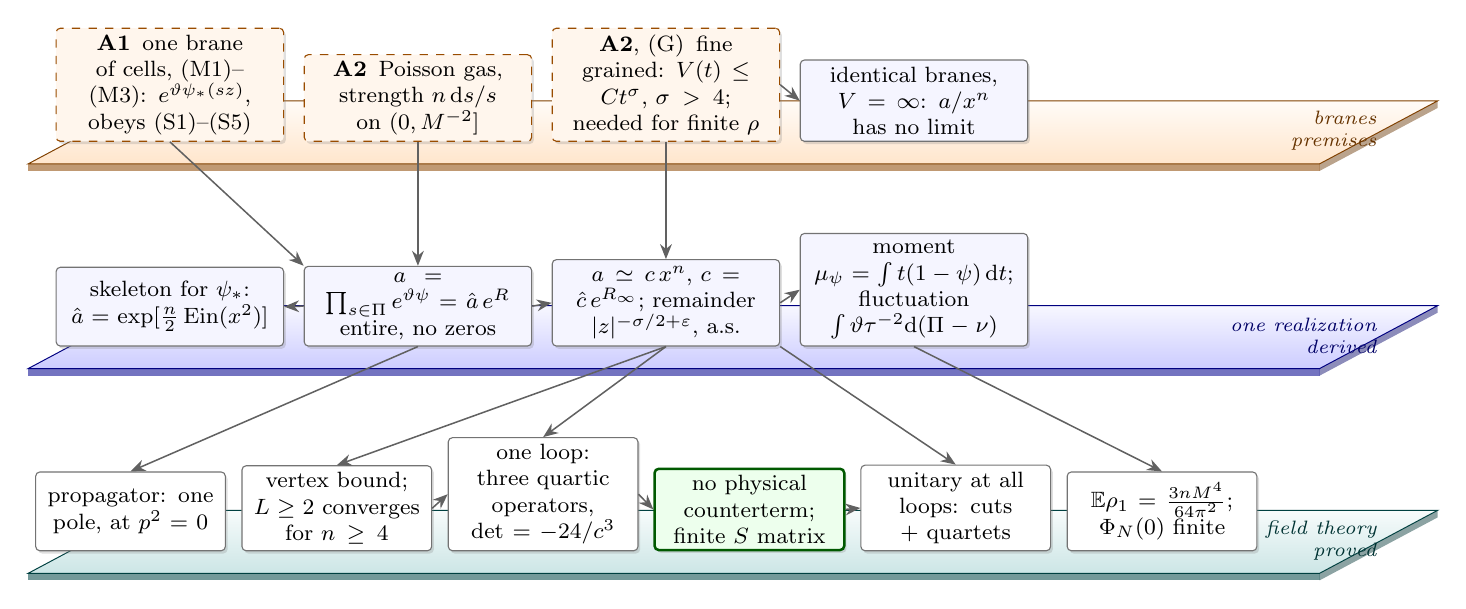
\begin{tikzpicture}[
  font=\footnotesize,
  box/.style={draw=black!55, line width=0.4pt, rounded corners=1.5pt, align=center, text width=#1, minimum height=1.0cm, inner sep=2.4pt, fill=white, drop shadow={shadow xshift=0.8pt, shadow yshift=-1.0pt, opacity=0.25}},
  box/.default=2.72cm,
  hyp/.style={box=#1, dashed, draw=orange!60!black, fill=orange!7},
  hyp/.default=2.72cm,
  der/.style={box=#1, fill=blue!4},
  der/.default=2.72cm,
  res/.style={box=2.24cm, fill=white},
  fin/.style={box=2.24cm, line width=0.9pt, draw=green!35!black, fill=green!7},
  arr/.style={-{Stealth[length=1.9mm,width=1.5mm]}, line width=0.55pt, black!62},
  ]
% slab: front-left corner (0,h), width W, depth vector (1.5,0.8), thickness 0.09
\newcommand{\slab}[3]{%
  \fill[#2!55!black, opacity=0.55] (0,#1-0.09) -- (16.4,#1-0.09) -- (16.4,#1) -- (0,#1) -- cycle;
  \fill[#2!40!black, opacity=0.45] (16.4,#1-0.09) -- (17.9,#1+0.71) -- (17.9,#1+0.8) -- (16.4,#1) -- cycle;
  \shade[top color=#2!3, bottom color=#2!20, draw=#2!50!black, line width=0.35pt]
    (0,#1) -- (16.4,#1) -- (17.9,#1+0.8) -- (1.5,#1+0.8) -- cycle;
  \node[anchor=east, align=right, font=\scriptsize\itshape, text=#2!40!black] at (17.25,#1+0.42) {#3};}
\slab{0}{teal}{field theory\\proved}
\slab{2.6}{blue}{one realization\\derived}
\slab{5.2}{orange}{branes\\premises}
% top layer: branes
\node[hyp, anchor=south] (A1)  at (1.8,5.48) {\textbf{A1}\enspace one brane of cells, (M1)--(M3): $e^{\vartheta\psi_*(sz)}$, obeys (S1)--(S5)};
\node[hyp, anchor=south] (gas) at (4.95,5.48) {\textbf{A2}\enspace Poisson gas, strength $n\,\dd s/s$ on $(0,M^{-2}]$};
\node[hyp, anchor=south] (G)   at (8.1,5.48) {\textbf{A2}, (G)\enspace fine grained: $V(t)\le Ct^{\sigma}$, $\sigma>4$; needed for finite $\rho$};
\node[der, anchor=south] (cex) at (11.25,5.48) {identical branes, $V=\infty$: $a/x^n$ has no limit};
% middle layer: one realization
\node[der, anchor=south] (ein)  at (1.8,2.88) {skeleton for $\psi_*$:\\ $\hat a=\exp[\frac n2\Ein(x^2)]$};
\node[der, anchor=south] (pgfl) at (4.95,2.88) {$a=\prod_{s\in\Pi}e^{\vartheta\psi}=\hat a\,e^{R}$\\ entire, no zeros};
\node[der, anchor=south] (gen)  at (8.1,2.88) {$a\simeq c\,x^n$, $c=\hat c\,e^{R_\infty}$; remainder $|z|^{-\sigma/2+\varepsilon}$, a.s.};
\node[der, anchor=south] (rho)  at (11.25,2.88) {moment $\mu_\psi=\int t(1-\psi)\,\dd t$; fluctuation $\int\vartheta\tau^{-2}\dd(\Pi-\nu)$};
% bottom layer: field theory
\node[res, anchor=south] (prop) at (1.3,0.28) {propagator: one pole, at $p^2=0$};
\node[res, anchor=south] (pc)   at (3.92,0.28) {vertex bound; $L\ge2$ converges for $n\ge4$};
\node[res, anchor=south] (one)  at (6.54,0.28) {one loop: three quartic operators, $\det=-24/c^3$};
\node[fin, anchor=south] (fin)  at (9.16,0.28) {no physical counterterm; finite $S$ matrix};
\node[res, anchor=south] (uni)  at (11.78,0.28) {unitary at all loops: cuts $+$ quartets};
\node[res, anchor=south] (vac)  at (14.4,0.28) {$\bE\rho_1=\frac{3nM^4}{64\pi^2}$; $\Phi_N(0)$ finite};
% arrows
\draw[arr] (A1.south) -- (pgfl.north west);
\draw[arr] (gas.south) -- (pgfl.north);
\draw[arr] (G.south) -- (gen.north);
\draw[arr] (G.east) -- (cex.west);
\draw[arr] (pgfl.west) -- (ein.east);
\draw[arr] (pgfl.east) -- (gen.west);
\draw[arr] (gen.east) -- (rho.west);
\draw[arr] (pgfl.south) -- (prop.north);
\draw[arr] (gen.south) -- (pc.north);
\draw[arr] (gen.south) -- (one.north);
\draw[arr] (gen.south east) -- (uni.north);
\draw[arr] (rho.south) -- (vac.north);
\draw[arr] (pc.east) -- (one.west);
\draw[arr] (one.east) -- (fin.west);
\draw[arr] (fin.east) -- (uni.west);
\end{tikzpicture}
\caption{Logical structure of the paper, in three layers. The top layer holds the premises about branes (dashed boxes): the response of one brane, A1, derived from a model of cells, and the gas, A2, whose fine-graining condition (G) is what lets a single realization carry the theory and is needed, up to factors slower than any power, for a finite zero-point energy; without it, for identical branes, the form factor has no power-law asymptotics (box on the right). The middle layer holds the properties of the form factor of one realization, derived for every admissible response and almost every realization (Secs.~\ref{sec:formfactor}--\ref{sec:fluct}), with the closed-form skeleton for $\psi_*$ as one instance. The bottom layer holds the field theory, which uses the form factor only through the middle layer and is proved for $n\ge4$; the box with the heavy frame is the main result. Arrows point from what is used to what is derived.}
\label{fig:logic}
\end{figure*}

\section{A gas of branes with no preferred size}
\label{sec:gas}

We work in Euclidean signature, with $z=p^2\ge0$ for real momenta, $\Box\to-p^2$, $x=z/M^2$ on the real axis and $w=z/M^2$ in the complex plane. Lorentzian statements follow by continuing $z$ to negative values; the response used for the closed forms depends on $z^2$, so for it the two half-axes behave alike.

\subsection{The response of one brane}
\label{sec:onebrane}

Consider a graviton mode crossing a stack of thin branes. Let $t_i$ and $r_i$ be the forward transmission and reflection amplitudes of brane $i$, and $\delta$ the phase accumulated between neighbors. Summing the multiple reflections between two branes gives $t_{12}=t_1t_2/(1-r_1'r_2e^{2i\delta})$, where $r_1'$ is the reflection amplitude of the first brane seen from the right. In the corresponding expansion for $N$ branes every term other than $\prod_it_i$ contains at least one round trip, and hence two reflection amplitudes, so that
\begin{equation}
\label{eq:compose}
t_{1\cdots N}=\Bigl(\prod_{i=1}^Nt_i\Bigr)\Bigl[1+O\Bigl(\sum_{i<j}|r_i||r_j|\Bigr)\Bigr].
\end{equation}
This is the composition rule of multiple scattering~\cite{Foldy1945,Lax1951}, written out for branes in Ref.~\cite{Bhattacharjee2026}. For weakly reflecting branes the kinetic operator of the graviton is dressed multiplicatively, $p^2\to p^2\prod_it_i^{-1}$, and the problem reduces to the single factor $t_i^{-1}$.\footnote{The gases below contain infinitely many branes, most of them much smaller than the wavelength of a given mode. The correction in Eq.~\eqref{eq:compose} is bounded by $(\sum_i|r_i|)^2$, which stays small if the reflection of a brane falls off for modes much longer than the brane at least as fast as its effect on the kinetic operator does. In the model of Sec.~\ref{sec:cells} there is no reflection, and the product is exact. The sum of the effects themselves converges almost surely (Sec.~\ref{sec:formfactor}).} We first state what the field theory requires of that factor, and call the requirement assumption A1. Sections~\ref{sec:class} and \ref{sec:uses} show that the field theory needs nothing more than these conditions, and Sec.~\ref{sec:cells} derives them from a model of the brane.

A brane has a size $s>0$, with dimensions of length squared, and a strength $\vartheta>0$, and it multiplies the spin-two and spin-zero parts of the graviton kinetic operator by
\begin{equation}
\label{eq:onebrane}
t^{-1}=e^{\vartheta\,\psi(sz)},
\end{equation}
where
\begin{enumerate}[label=\textup{(S\arabic*)},leftmargin=2.4em,itemsep=0.15em]
\item $\psi$ is entire and $\psi(0)=0$;
\item $\psi$ is real on the real axis, with $0\le\psi(t)\le1$ there;
\item $1-\psi$ and all its derivatives decay along the real axis faster than any power of $1/|t|$;
\item the decay in (S3) holds uniformly in closed sectors around the real axis: there is an opening $\theta>0$ such that for every $\delta\in(0,\theta)$ and every $N$, $|1-\psi(w)|\le C_{\delta,N}|w|^{-N}$ for $|w|\ge1$ and $|\arg(\pm w)|\le\theta-\delta$.
\end{enumerate}
On the real axis the factor~\eqref{eq:onebrane} rises from $1$, for modes much longer than the brane, to $e^{\vartheta}$, for modes much shorter, so $\vartheta$ is the saturated logarithmic strength of the brane. Condition (S1) says that a brane has a single length scale and leaves long modes untouched. Condition (S2) is passivity: along the real axis, spacelike and timelike alike, a brane can suppress a mode but never amplify it. Condition (S3) says that the suppression saturates once the mode is much shorter than the brane. Condition (S4) says that saturation is not special to real momenta: a mode whose squared momentum is slightly complex, as it is for the loop energies of Sec.~\ref{sec:unitarity} near the ends of their contours, is saturated as well.\footnote{Condition (S4) does not follow from (S3). The entire function $\psi(w)=1-e^{-w^2}\cos^2(e^w-1)$ satisfies (S1)--(S3), but off the real axis $|\cos^2(e^w-1)|$ grows like $\exp(2e^{\mathrm{Re}\,w}|\sin\mathrm{Im}\,w|)$, which defeats the Gaussian in every sector. For the response $\psi_*$ used below the opening is $\theta=\pi/4$.} Dependence on the momentum through $p^2$ alone requires the branes to respect four-dimensional Poincar\'e invariance, as branes that fill the observed four dimensions and are scattered in the transverse ones do.

The exponential in Eq.~\eqref{eq:onebrane} is not a separate choice. It is equivalent to a fifth condition,
\begin{enumerate}[label=\textup{(S5)},leftmargin=2.4em,itemsep=0.15em]
\item the factor $t^{-1}$ has no zeros in the complex plane of $z$,
\end{enumerate}
which says that a brane has no resonances: a zero of $t^{-1}$ is a pole of the transmission amplitude at complex momentum, a quasi-bound state of the brane. Suppose a brane multiplies the kinetic operator by $1+\varphi(sz)$, with $\varphi$ entire, real on the real axis, $\varphi(0)=0$, and $0\le\varphi\le\varphi_\infty$ on the real axis, saturating at $\varphi_\infty$ as in (S3) and (S4). If $1+\varphi$ has no zeros it is the exponential of an entire function, $1+\varphi=e^{h}$ with $h(0)=0$~\cite{Titchmarsh1939}, and $h=\log(1+\varphi)$ on the real axis, where $1+\varphi>0$. Put $\vartheta=\log(1+\varphi_\infty)$ and $\psi=h/\vartheta$. Then $\psi$ satisfies (S1) and (S2), and $1-\psi=-\vartheta^{-1}\log[1-(\varphi_\infty-\varphi)/(1+\varphi_\infty)]$ is bounded by $2|\varphi_\infty-\varphi|/\vartheta$ wherever $|\varphi_\infty-\varphi|\le\frac12(1+\varphi_\infty)$, which gives (S3) and (S4).\footnote{In a sector, at large $|w|$, $h-\vartheta$ equals the principal logarithm of $(1+\varphi)/(1+\varphi_\infty)$ plus $2\pi i k$ with an integer $k$ that is constant on the connected set where the ratio is close to $1$; that set touches the real axis, where $k=0$.} Conversely $e^{\vartheta\psi}$ is entire and has no zeros. Conditions (S1)--(S5) on a factor $1+\varphi$ are therefore the same as (S1)--(S4) on the exponent $\psi$ of Eq.~\eqref{eq:onebrane}.

Condition (S5) is what lets a single realization of the gas define a theory, and it fails for the most obvious saturating factor. The function $1+\varphi=2-e^{-s^2z^2}$ obeys every other condition, but it vanishes when
\begin{equation}
\label{eq:qzeros}
s^2z^2=-\log2-2\pi ik,\qquad k\in\mathbb Z .
\end{equation}
These resonances lie in $\pi/4<|\arg z|<3\pi/4$, away from both real half-axes, but there are infinitely many of them, and a product over a gas of such branes vanishes at the resonances of every brane in it. A gas with $n$ such branes per $e$-fold of size below $1/M^2$ has on average $nR^2/(\pi M^4)$ zeros in the disk $|z|<R$ for $R\gg M^2$,\footnote{A brane of size $s$ contributes the zeros with $|\log2+2\pi ik|\le s^2R^2$ inside the disk $|z|\le R$, about $2s^2R^2/\pi$ of them counting both signs of $z$. Averaging with $n\,\dd s/s$ over $s\le M^{-2}$ gives $nR^2/(\pi M^4)$. The numerical check in Appendix~\ref{app:checks} reproduces this count to $0.03\%$ at $R=60M^2$.} each a complex pole of the propagator. Complex pairs of this kind are what Lee and Wick~\cite{LeeWick1969} and, in a modern form, Anselmi and Piva~\cite{Anselmi2017,AnselmiPiva2017} proposed to treat with a modified prescription. Branes obeying (S5) have none, and no such prescription is needed.

The simplest response with all five properties, and the one we use from Sec.~\ref{sec:closed} on, has the exponent
\begin{equation}
\label{eq:phistar}
\psi_*(w)=1-e^{-w^2},\qquad t^{-1}=\exp\bigl[\vartheta\bigl(1-e^{-s^2z^2}\bigr)\bigr].
\end{equation}
Its derivative expansion is $t^{-1}=1+\vartheta s^2z^2+O(z^4)$. The more obvious exponent $1-e^{-w}$, which would give the incomplete gamma function directly, violates (S2): on the negative axis it is unbounded below, so the factor falls to zero faster than any power along the timelike axis and no polynomial bound holds there.\footnote{The exponent of the gas, computed as in Sec.~\ref{sec:formfactor}, is then $n\Ein(z/M^2)$, and along the negative real axis $\Ein(-t)=-\int_0^t(e^{u}-1)\,\dd u/u$ tends to $-\infty$ faster than any power. Passivity keeps the two half-axes symmetric.}

Conditions (S1) and (S2) already have a consequence. On the real axis $\psi\ge0=\psi(0)$, so the origin is a minimum of a smooth function and $\psi'(0)=0$. The leading correction that a passive brane makes to the kinetic operator is therefore of order $s^2z^2$ and not $sz$: a passive brane does not generate a curvature-squared term at leading order.

\subsection{A brane made of cells}
\label{sec:cells}

Conditions (S1)--(S5) say what a brane must do. A simple model of what a brane is made of produces all five, and it produces the response $\psi_*$ of Eq.~\eqref{eq:phistar} instead of leaving it as a choice. Take a brane of size $s$ to be a thin layer of microscopic cells, and assume three things about them.
\begin{enumerate}[label=\textup{(M\arabic*)},leftmargin=2.4em,itemsep=0.15em]
\item The cells are placed independently of one another, so that a mode crossing the brane at a given point of its worldvolume meets a Poisson number $N$ of cells, with a mean $\vartheta$ that is the same at every point.
\item A cell neither absorbs nor reflects. It shifts the proper time of the mode that crosses it by an amount $Y$, a delay or an advance.
\item The shifts of different cells are independent, with a common law that is Gaussian with mean zero and variance $2s^2$.
\end{enumerate}
The first assumption is the independence that made the gas a Poisson process, applied now inside one brane. The second fixes how a cell acts. In the proper-time representation of the propagator a mode of squared momentum $z$ propagates for a proper time $T$ with the amplitude $e^{-iTz}$, so a shift of $T$ by $Y$ multiplies it by the phase $e^{-iYz}$, of modulus one for real $z$ of either sign.\footnote{With the Euclidean $z=p^2$ of this section, a Lorentzian mode of squared four-momentum $-z$ has the proper-time amplitude $e^{iT(-z+i0)}$, and the propagator is its integral over $T\ge0$. Whether a cell multiplies the amplitude by $e^{-iYz}$ or $e^{iYz}$ is a convention that the symmetry of the law in (M3) makes irrelevant.} On shell, $z=0$, the phase is $1$: a cell does not act on a free graviton, as it must not if the brane is invariant under the Poincar\'e group of its worldvolume. Off shell the phases of the cells that a mode crosses add up. The third assumption is what the central limit theorem gives when the shift of a cell is the sum of many small independent shifts of its constituents, and the symmetry $Y\to-Y$ says that a cell has no preferred direction of proper time. The size of the brane is the spread of the shift, $\bE Y^2=2s^2$, which is why $s$ has the dimensions of a proper time, a length squared.

A mode crossing the brane is a plane wave across its worldvolume, and different points of the worldvolume meet independent sets of cells. What continues as the same mode is the coherent part of the transmitted wave, the average of the phase over the worldvolume; the remainder is scattered into other modes. This is the coherent wave of the theory of multiple scattering~\cite{Foldy1945,Lax1951}, and Fig.~\ref{fig:cells} shows the construction. For a brane whose extent is large compared with the spacing of its cells, the average over the worldvolume is the expectation over the cells, by the law of large numbers. Conditioning on $N$,
\begin{align}
t&=\bE\exp\Bigl(-iz\sum_{j=1}^NY_j\Bigr)=\sum_{N\ge0}e^{-\vartheta}\frac{\vartheta^N}{N!}\,\varphi(sz)^N\nonumber\\
&=e^{-\vartheta[1-\varphi(sz)]},\label{eq:cellt}
\end{align}
where $\varphi(u)=\bE\,e^{-iuY/s}$ is the characteristic function of $Y/s$. For the Gaussian law of (M3), $\varphi(u)=e^{-u^2}$, and Eq.~\eqref{eq:cellt} is the single-brane factor~\eqref{eq:onebrane} with
\begin{equation}
\label{eq:cellpsi}
\psi(w)=1-\varphi(w)=1-e^{-w^2}=\psi_*(w).
\end{equation}
The response used from Sec.~\ref{sec:closed} on is therefore the response of a brane whose cells shift the proper time by Gaussian amounts, and the strength $\vartheta$ is the mean number of cells that a mode meets, the optical depth of the brane.

All five conditions follow. The exponent $\vartheta\psi$ is entire, so $t^{-1}$ has no zeros, which is (S5); in the model a resonance would need a cell that holds the mode, and (M2) excludes it. Condition (S1) holds because $\varphi(0)=1$. The law is symmetric, so $\varphi$ is real on the real axis, and for the Gaussian $0<\varphi\le1$ there, which gives $0\le\psi<1$, condition (S2). Passivity is now the statement that the coherent wave can only lose amplitude to the scattered one, $|t|\le1$. On the real axis $1-\psi=e^{-w^2}$ falls faster than any power, which is (S3), and $|e^{-w^2}|=e^{-\mathrm{Re}\,w^2}$ falls in the same way in every closed subsector of $|\arg(\pm w)|<\pi/4$, which is (S4) with $\theta=\pi/4$. For modes much shorter than the brane, $t\to e^{-\vartheta}$, the probability of meeting no cell. Finally, since cells do not reflect and are independent of the cells of other branes, the coherent amplitude through several branes is the product of their amplitudes, with no correction: the composition rule~\eqref{eq:compose} holds exactly, with $r_i=0$.

Other laws for the shift give other responses, $\psi=1-\varphi$ with $\varphi$ the characteristic function of a symmetric law, and conditions (S1)--(S5) then ask that $\varphi$ be entire, nonnegative on the real axis, and rapidly decreasing in a sector. A Gaussian whose variance is itself random, between two positive bounds, passes all of them, again with $\theta=\pi/4$. A law with bounded support does not: its characteristic function is entire of exponential type and grows off the real axis, which defeats (S4). Of the admissible exponents of Sec.~\ref{sec:class}, the other two in Table~\ref{tab:class} are not of the form $1-\varphi$ at all, since $(1+w^2)e^{-w^2}$ and $e^{-w^4}$ have Fourier transforms that take negative values and are therefore not characteristic functions. We do not derive (M1)--(M3) from a brane action. What the model does is replace five conditions on an unknown function by three statements about the constituents of a brane, each with a physical meaning, and with them the single-brane factor is computed rather than chosen.

\begin{figure}[t]
\centering
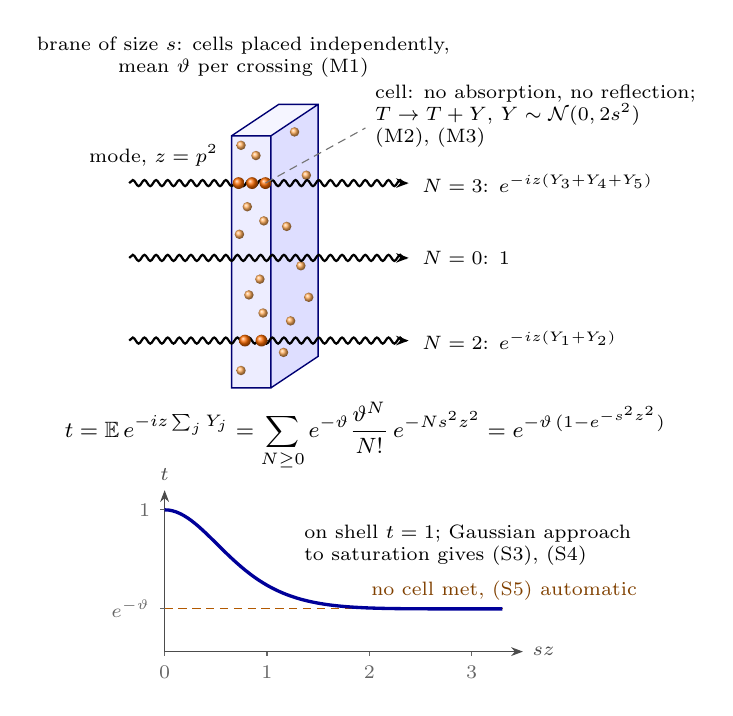
\begin{tikzpicture}[font=\footnotesize,x=1cm,y=1cm]
% the brane: a thin layer seen in perspective
\fill[blue!7] (1.6,0) -- (2.1,0) -- (2.1,3.2) -- (1.6,3.2) -- cycle;
\fill[blue!13] (2.1,0) -- (2.7,0.4) -- (2.7,3.6) -- (2.1,3.2) -- cycle;
\fill[blue!4] (1.6,3.2) -- (2.1,3.2) -- (2.7,3.6) -- (2.2,3.6) -- cycle;
\draw[blue!45!black,line width=0.5pt] (1.6,0) -- (2.1,0) -- (2.1,3.2) -- (1.6,3.2) -- cycle (2.1,0) -- (2.7,0.4) -- (2.7,3.6) -- (2.2,3.6) -- (1.6,3.2) (2.1,3.2) -- (2.7,3.6);
% cells off the three paths
\foreach \x/\y in {1.72/0.22,2.00/0.95,1.82/1.18,1.96/1.38,1.70/1.95,2.01/2.12,1.80/2.30,1.91/2.95,1.72/3.08,2.35/0.85,2.48/1.55,2.30/2.05,2.55/2.70,2.40/3.25,2.26/0.45,2.58/1.15}
  {\shade[ball color=orange!65] (\x,\y) circle (0.06);}
% three crossing points: two cells, none, three cells
\draw[grav,-{Stealth[length=1.6mm]}] (0.3,0.6) -- (3.85,0.6);
\draw[grav,-{Stealth[length=1.6mm]}] (0.3,1.65) -- (3.85,1.65);
\draw[grav,-{Stealth[length=1.6mm]}] (0.3,2.6) -- (3.85,2.6);
\foreach \x/\y in {1.77/0.6,1.98/0.6,1.69/2.6,1.86/2.6,2.03/2.6}
  {\shade[ball color=orange!85!red] (\x,\y) circle (0.075);}
\node[anchor=west,font=\scriptsize] at (3.9,0.6) {$N=2$: $e^{-iz(Y_1+Y_2)}$};
\node[anchor=west,font=\scriptsize] at (3.9,1.65) {$N=0$: $1$};
\node[anchor=west,font=\scriptsize] at (3.9,2.6) {$N=3$: $e^{-iz(Y_3+Y_4+Y_5)}$};
\node[anchor=east,font=\scriptsize] at (1.55,2.95) {mode, $z=p^2$};
\node[font=\scriptsize,align=center] at (1.75,4.2) {brane of size $s$: cells placed independently,\\ mean $\vartheta$ per crossing (M1)};
\draw[densely dashed,black!55] (2.03,2.6) -- (3.3,3.3);
\node[anchor=west,font=\scriptsize,align=left] at (3.3,3.45) {cell: no absorption, no reflection;\\ $T\to T+Y$, $Y\sim\mathcal N(0,2s^2)$\\ (M2), (M3)};
% the coherent average
\node[font=\footnotesize] at (3.3,-0.62) {$t=\bE\,e^{-iz\sum_jY_j}=\displaystyle\sum_{N\ge0}e^{-\vartheta}\frac{\vartheta^N}{N!}\,e^{-Ns^2z^2}=e^{-\vartheta\,(1-e^{-s^2z^2})}$};
% t against sz
\begin{scope}[shift={(0.75,-3.35)}]
\draw[-{Stealth[length=1.5mm]},black!70] (0,0) -- (4.55,0) node[right,font=\scriptsize] {$sz$};
\draw[-{Stealth[length=1.5mm]},black!70] (0,0) -- (0,2.05) node[above,font=\scriptsize] {$t$};
\foreach \u in {0,1,2,3} {\draw[black!60] (1.3*\u,0) -- ++(0,-0.06) node[below,font=\scriptsize] {$\u$};}
\draw[black!60] (0,1.8) -- ++(-0.06,0) node[left,font=\scriptsize] {$1$};
\draw[black!60] (0,0.542) -- ++(-0.06,0) node[left,font=\scriptsize] {$e^{-\vartheta}$};
\draw[densely dashed,orange!70!black] (0,0.542) -- (4.3,0.542);
\draw[very thick,blue!60!black,domain=0:3.3,samples=90] plot ({1.3*\x},{1.8*exp(-1.2*(1-exp(-\x*\x)))});
\node[font=\scriptsize,align=left,anchor=west] at (1.65,1.35) {on shell $t=1$; Gaussian approach\\ to saturation gives (S3), (S4)};
\node[font=\scriptsize,anchor=west,orange!50!black] at (2.5,0.78) {no cell met, (S5) automatic};
\end{scope}
\end{tikzpicture}
\caption{A brane made of cells, Sec.~\ref{sec:cells}. A mode of squared momentum $z$ crosses a brane of size $s$ at every point of its worldvolume. At each point it meets a Poisson number $N$ of cells with mean $\vartheta$, (M1), each of which shifts its proper time by an independent Gaussian amount $Y_j$ of variance $2s^2$, (M2) and (M3), and so multiplies it by the phase $e^{-iY_jz}$. Three crossing points are drawn, which meet, from bottom to top, two, zero and three cells. The coherent transmitted wave is the average of the phase, Eq.~\eqref{eq:cellt}, which is the single-brane factor~\eqref{eq:onebrane} with $\psi=\psi_*$, Eq.~\eqref{eq:cellpsi}. Lower panel: $t$ as a function of $sz$ for $\vartheta=1.2$. It equals $1$ on shell and falls to the saturation value $e^{-\vartheta}$, the probability that a crossing meets no cell, as the mode becomes shorter than the brane.}
\label{fig:cells}
\end{figure}

\subsection{Sizes and strengths}
\label{sec:sizes}

A gas is a random set of branes, each with a size and a strength. We impose three requirements on it: branes are placed independently of one another; below the size $S=1/M^2$ of the largest brane there is no preferred size; and the strength of the gas is fine grained, in a sense made precise below. Together they form assumption A2.

The first requirement makes the set of sizes a Poisson process. A point process without multiple points and without fixed atoms, whose counts in disjoint sets are independent, is a Poisson process with some intensity measure $\nu$~\cite{Kingman1993,LastPenrose2017}.\footnote{This is the theorem of R\'enyi and Kingman: complete independence plus simplicity characterizes the Poisson process. The intensity measure $\nu(A)$ is the expected number of branes with size in $A$.} We let the strength depend on the size, $\vartheta=\vartheta(s)$.\footnote{Strengths drawn independently from a law that depends on $s$ make the gas a marked Poisson process~\cite{Kingman1993}. The mean and variance formulas below then hold with $\vartheta$ and $\vartheta^2$ replaced by their conditional means at fixed $s$, and the exponential formulas with $e^{h}$ replaced by its conditional mean.}

The second requirement concerns the quantity that enters the kinetic operator, which is the strength. The expected strength carried by the branes with sizes in a set $A$, $\int_A\vartheta\,\dd\nu$, must not change under a dilation $s\to\lambda s$ whenever both $A$ and $\lambda A$ lie in $(0,S]$. In the variable $u=\log s$ this is invariance under translations along the half-line $u\le\log S$, so the measure of an interval depends only on its length; it is additive and monotone in that length, hence linear in it, and $\vartheta\,\dd\nu$ is a multiple of Lebesgue measure in $u$.\footnote{Additivity gives $\mu(h_1+h_2)=\mu(h_1)+\mu(h_2)$ for the measure $\mu(h)$ of an interval of length $h$, and a monotone solution of Cauchy's equation is linear. This is the uniqueness of Haar measure on the multiplicative group $(0,\infty)$, restricted to the cut-off range.} Therefore
\begin{equation}
\label{eq:intensity}
\vartheta(s)\,\nu(\dd s)=n\,\frac{\dd s}{s}\quad\text{on }(0,S],\qquad n>0 ,
\end{equation}
and $n$ is the expected strength per $e$-fold of size. For identical branes, $\vartheta=\vartheta_0$, this says that the number of branes per $e$-fold, $n/\vartheta_0$ on average, is the same at all sizes.

The third requirement is about how that strength is shared. It can be carried by a few strong branes or by many weak ones. Write $\tau=sM^2\in(0,1]$ and
\begin{equation}
\label{eq:V}
V(t)=\frac1n\int_{\tau\le t}\vartheta^2\,\dd\nu=\int_0^t\vartheta(\tau)\,\frac{\dd\tau}\tau .
\end{equation}
We show in Sec.~\ref{sec:avg} that $nV(t)$ is the variance of the strength carried by the branes smaller than $t/M^2$, measured from its mean. The requirement is
\begin{enumerate}[label=\textup{(G)},leftmargin=2.4em,itemsep=0.15em]
\item $V(t)\le C\,t^{\sigma}$ for $0<t\le1$, with some $\sigma>4$.
\end{enumerate}
In words: the fluctuation of the strength carried by small branes vanishes with their size faster than $(\text{size})^{2}$. It does not affect the mean, which Eq.~\eqref{eq:intensity} fixes. The exponent is not chosen to make the proofs below work. Section~\ref{sec:vacuum} shows that the zero-point energy of a single realization has a value that is the same for every regulator only if the fluctuation falls at least this fast: when smaller branes are never stronger, it needs $V(t)=o(t^4)$, so (G) is necessary up to factors that vary more slowly than any power of $t$. Sections~\ref{sec:fluct}--\ref{sec:oneloop} show that (G) is also all the field theory needs. The simplest example is a power law,
\begin{equation}
\label{eq:finegrain}
\vartheta(\tau)=\vartheta_0\,\tau^{\zeta},\qquad\nu(\dd\tau)=\frac n{\vartheta_0}\,\tau^{-\zeta}\,\frac{\dd\tau}\tau,\qquad V(t)=\frac{\vartheta_0t^{\zeta}}\zeta ,
\end{equation}
for which (G) holds with $\sigma=\zeta$ when $\zeta>4$. As the size decreases by one $e$-fold the branes become weaker by a factor $e^{-\zeta}$ and $e^{\zeta}$ times as numerous, so the strength per $e$-fold stays $n$ while the gas becomes ever finer. Any profile that falls faster than every power, such as $\vartheta_0\exp[-(\log\tau)^2]$, satisfies (G) for every $\sigma$. A gas of identical branes, $\zeta=0$, has $V\equiv\infty$ and violates (G) completely; Sec.~\ref{sec:fluct} shows what goes wrong with it. Figure~\ref{fig:gas}(a) shows the two kinds of gas, and Fig.~\ref{fig:finegrain} shows the bookkeeping.

\begin{figure}[t]
\centering
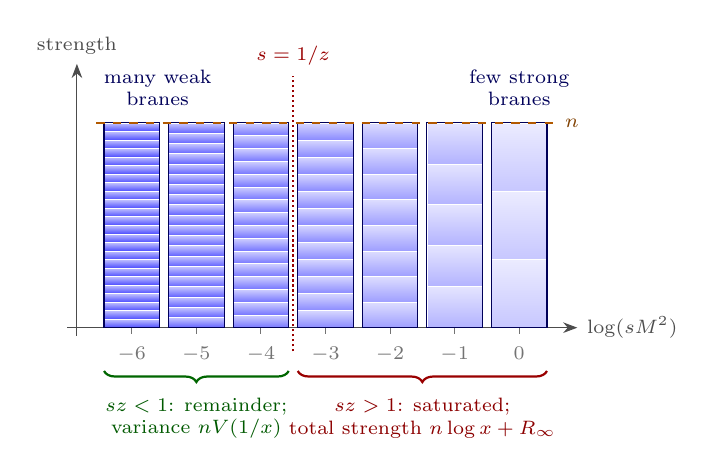
\begin{tikzpicture}[font=\footnotesize,x=0.82cm,y=1cm]
\def\H{2.6}
% axes
\draw[-{Stealth[length=1.8mm]},black!70] (-0.15,0) -- (7.75,0) node[right,font=\scriptsize] {$\log(sM^2)$};
\draw[-{Stealth[length=1.8mm]},black!70] (0,-0.1) -- (0,3.35) node[above,font=\scriptsize] {strength};
\foreach \k/\lab in {0/{-6},1/{-5},2/{-4},3/{-3},4/{-2},5/{-1},6/{0}} \draw[black!55] (\k+0.85,0) -- ++(0,-0.08) node[below=1pt,font=\scriptsize] {$\lab$};
% columns: each e-fold carries total strength n (height H), split into m slabs
\foreach \k/\m/\col in {0/24/blue!70,1/20/blue!62,2/16/blue!54,3/12/blue!46,4/8/blue!38,5/5/blue!30,6/3/blue!22} {
  \pgfmathsetmacro{\dh}{\H/\m}
  \foreach \j in {1,...,\m} {
    \pgfmathsetmacro{\yy}{(\j-1)*\dh}
    \shade[top color=white!65!\col, bottom color=\col, draw=white, line width=0.25pt] (\k+0.42,\yy) rectangle (\k+1.28,\yy+\dh);
  }
  \draw[blue!35!black,line width=0.4pt] (\k+0.42,0) rectangle (\k+1.28,\H);
}
\draw[dashed,orange!70!black,thick] (0.3,\H) -- (7.4,\H) node[right,font=\scriptsize,text=orange!50!black,align=left] {$n$};
\node[font=\scriptsize,align=center,text=blue!35!black] at (6.85,3.05) {few strong\\ branes};
\node[font=\scriptsize,align=center,text=blue!35!black] at (1.25,3.05) {many weak\\ branes};
% brace for branes larger than 1/z
\draw[decorate,decoration={brace,amplitude=4pt,mirror},thick,red!60!black] (3.42,-0.55) -- (7.28,-0.55);
\node[red!55!black,font=\scriptsize,align=center] at (5.35,-1.15) {$sz>1$: saturated;\\ total strength $n\log x+R_\infty$};
\draw[decorate,decoration={brace,amplitude=4pt,mirror},thick,green!40!black] (0.42,-0.55) -- (3.28,-0.55);
\node[green!35!black,font=\scriptsize,align=center] at (1.85,-1.15) {$sz<1$: remainder;\\ variance $nV(1/x)$};
\draw[red!60!black,densely dotted,thick] (3.35,-0.3) -- (3.35,3.2) node[above,font=\scriptsize] {$s=1/z$};
\end{tikzpicture}
\caption{How a fine-grained gas shares its strength. Each column is one $e$-fold of size and carries expected strength $n$ (dashed line), Eq.~\eqref{eq:intensity}. The number of branes in a column, drawn as slabs, grows toward small sizes while each slab gets thinner, as for the power law~\eqref{eq:finegrain}. A mode with $z=p^2$ saturates the branes larger than $1/z$, whose total strength is $n\log x$ plus a fluctuation that converges to $R_\infty$; the branes smaller than $1/z$ act only through a remainder whose variance is $nV(1/x)$ (Sec.~\ref{sec:fluct}).}
\label{fig:finegrain}
\end{figure}

\subsection{Sums and products over the gas}
\label{sec:avg}

Because the gas has infinitely many points, we derive the formulas we need instead of quoting them. Let $\Pi$ be a Poisson process with $\sigma$-finite intensity $\nu$ and let $f$ be a complex function with $\int|f|\,\dd\nu<\infty$. Then
\begin{equation}
\label{eq:pgfl}
\bE\prod_{x\in\Pi}\bigl(1+f(x)\bigr)=\exp\int f\,\dd\nu ,
\end{equation}
with the product converging absolutely almost surely. Suppose first that the total mass $\lambda=\nu(\text{all})$ is finite. The number $N$ of points is then Poisson with mean $\lambda$, and given $N$ the points are independent with law $\nu/\lambda$~\cite{LastPenrose2017}. Conditioning on $N$,
\begin{align*}
\bE\prod_{x\in\Pi}(1+f)&=\sum_{N\ge0}e^{-\lambda}\frac{\lambda^N}{N!}\Bigl(\frac1\lambda\int(1+f)\,\dd\nu\Bigr)^{N}\\
&=e^{-\lambda}e^{\lambda+\int f\,\dd\nu},
\end{align*}
which is Eq.~\eqref{eq:pgfl}; the same computation with $|f|$ in place of $f$ gives $\bE\prod(1+|f|)=\exp\int|f|\,\dd\nu$, so the expectation exists. If $\nu$ has infinite mass, choose sets $A_1\subset A_2\subset\cdots$ of finite measure that exhaust the space. Campbell's theorem, $\bE\sum_{x\in\Pi}g(x)=\int g\,\dd\nu$ for $g\ge0$~\cite{Kingman1993}, applied to $g=|f|$, shows that $\sum_{x\in\Pi}|f(x)|<\infty$ almost surely, so the product converges absolutely and is the limit of the products over $\Pi\cap A_k$. These partial products are bounded in modulus by $\prod_{x\in\Pi}(1+|f(x)|)$, whose expectation is $\exp\int|f|\,\dd\nu$ by monotone convergence and the finite case. Dominated convergence then gives $\bE\prod_{x\in\Pi}(1+f)=\lim_k\exp\int_{A_k}f\,\dd\nu=\exp\int f\,\dd\nu$.

Two consequences are used below. Replace $f$ by $e^{uf}-1$ with real $f$ and real $u$ in the finite case and differentiate twice at $u=0$: the sum $\sum_{x\in\Pi}f(x)$ has mean $\int f\,\dd\nu$ and variance $\int f^2\,\dd\nu$. For complex $f$, applying this to the real and imaginary parts and to their sum gives
\begin{equation}
\label{eq:isometry}
\bE\Bigl|\sum_{x\in\Pi}f(x)-\int f\,\dd\nu\Bigr|^2=\int|f|^2\,\dd\nu .
\end{equation}
Write the left side as $\bE|\int f\,\dd(\Pi-\nu)|^2$. If $\int|f|^2\dd\nu<\infty$ but $\int|f|\,\dd\nu=\infty$, the compensated sums over $\Pi\cap A_k$ still converge: their increments over $A_{k+1}\setminus A_k$ are independent, have mean zero and have summable variances, so they converge almost surely and in mean square by Kolmogorov's criterion~\cite{Feller1971}. We call the limit $\int f\,\dd(\Pi-\nu)$; it has mean zero and obeys Eq.~\eqref{eq:isometry}. With $f=\vartheta$ on the branes smaller than $t/M^2$ and $f=0$ elsewhere, Eq.~\eqref{eq:isometry} shows that $nV(t)$, Eq.~\eqref{eq:V}, is the variance of their total strength measured from its mean. The same exhaustion applied to Eq.~\eqref{eq:pgfl} with $f=e^{h}-1$ gives, for real $h$ with $|h|\le h_{\max}$ and $\int h^2\dd\nu<\infty$,
\begin{equation}
\label{eq:expmoment}
\bE\exp\int h\,\dd(\Pi-\nu)=\exp\int\bigl(e^{h}-1-h\bigr)\,\dd\nu .
\end{equation}
On each $A_k$ this is Eq.~\eqref{eq:pgfl} with $f=e^h-1$, multiplied by $\exp(-\int_{A_k}h\,\dd\nu)$. The integrand on the right is at most $\frac12e^{h_{\max}}h^2$, so the right side is finite, and the same bound with $2h$ in place of $h$ shows that $\bE\exp\bigl(2\int_{A_k}h\,\dd(\Pi-\nu)\bigr)\le\exp\bigl(2e^{2h_{\max}}\int h^2\dd\nu\bigr)$ uniformly in $k$. The exponentials are therefore uniformly integrable, and their means converge to the mean of the limit.

\subsection{The form factor of one realization}
\label{sec:formfactor}

A realization $\Pi$ of the gas is one draw of the branes, frozen. A graviton crossing it is dressed by the product of the factors~\eqref{eq:onebrane} of all its branes,
\begin{equation}
\label{eq:aPi}
\begin{gathered}
a_\Pi(z)=\prod_{s\in\Pi}e^{\vartheta(s)\psi(sz)}=\exp L_\Pi(z),\\
L_\Pi(z)=\sum_{s\in\Pi}\vartheta(s)\,\psi(sz).
\end{gathered}
\end{equation}
The sum converges. Because $\psi$ is entire and vanishes at the origin, $|\psi(w)|\le A_R|w|$ on the disk $|w|\le R$, and with Eq.~\eqref{eq:intensity} Campbell's theorem gives
\[
\begin{aligned}
\bE\sum_{s\in\Pi}\sup_{|z|\le RM^2}\bigl|\vartheta(s)\psi(sz)\bigr|&\le n\int_0^1A_RR\tau\,\frac{\dd\tau}\tau\\
&=nA_RR<\infty .
\end{aligned}
\]
Almost surely, then, the sum in Eq.~\eqref{eq:aPi} converges absolutely and uniformly on every disk, its limit $L_\Pi$ is an entire function, and $a_\Pi=e^{L_\Pi}$ is an entire function \emph{without zeros}. It satisfies $a_\Pi(0)=1$, its Taylor coefficients are real, and $a_\Pi\ge1$ on the whole real axis by (S2). A frozen gas of branes that obey (S5) therefore has no extra poles of any kind, real or complex. Condition (S5) is necessary as well as sufficient for this: if one factor vanished at some $z_0$, the convergent product of the others would be finite there and $a_\Pi(z_0)$ would vanish.

The mean of the exponent is fixed by Eq.~\eqref{eq:intensity} alone. By Campbell's theorem, $\bE L_\Pi(z)=\int\vartheta\,\psi(sz)\,\dd\nu=n\int_0^{1/M^2}\psi(sz)\,\dd s/s$, and the substitution $s=\tau/M^2$ gives
\begin{equation}
\label{eq:split}
\begin{gathered}
a_\Pi(z)=e^{n\Phi(z/M^2)}\,e^{R_\Pi(z)},\\
R_\Pi(z)=\int\vartheta(s)\,\psi(sz)\,(\Pi-\nu)(\dd s),
\end{gathered}
\end{equation}
\begin{equation}
\label{eq:Phi}
\Phi(w)=\int_0^1\psi(w\tau)\,\frac{\dd\tau}{\tau}=\sum_{k\ge1}\frac{\psi_k}{k}\,w^k ,
\end{equation}
where $\psi(w)=\sum_{k\ge1}\psi_kw^k$. The first factor in Eq.~\eqref{eq:split} is deterministic. It depends on the gas only through $n$ and not at all on how the strength is shared among branes; we call
\begin{equation}
\label{eq:avg}
\hat a(z)=\exp\Bigl[n\,\Phi\Bigl(\frac z{M^2}\Bigr)\Bigr]
\end{equation}
the skeleton of the form factor. The second factor is random, with $\bE R_\Pi(z)=0$; it is the subject of Sec.~\ref{sec:fluct}. The skeleton is the exponential of the mean of $\log a_\Pi$. It is not the mean of $a_\Pi$, which for real $z$ and bounded strengths is, by Eq.~\eqref{eq:expmoment}, $\hat a$ times $\exp\int(e^{\vartheta\psi}-1-\vartheta\psi)\,\dd\nu$, and nothing in this paper averages the kinetic operator over the gas. The graviton sees one realization, and the theory is that of $a_\Pi$.

The Taylor series of $\psi$ converges uniformly on $\{|w\tau|\le R\}$ and may be integrated term by term, and since the coefficients of $\Phi$ are bounded by those of $\psi$ its radius of convergence is infinite. So $\Phi$ is entire with $\Phi(0)=0$, and $\hat a$ is entire, has no zeros and satisfies $\hat a(0)=1$.

The growth of the skeleton on the real axis follows from (S3). For real $x>0$, $\Phi(x)=\int_0^x\psi(t)\,\dd t/t$. Splitting the range at $t=1$ and writing $\psi=1-(1-\psi)$ on $[1,x]$,
\begin{equation}
\label{eq:Phi-asym}
\Phi(x)=\log|x|+C_\pm+\rho_\pm(x),\qquad x\to\pm\infty,
\end{equation}
with
\begin{align*}
C_\pm&=\int_0^1\psi(\pm t)\frac{\dd t}t-\int_1^\infty\bigl(1-\psi(\pm t)\bigr)\frac{\dd t}t,\\
\rho_\pm(x)&=\int_{|x|}^\infty\bigl(1-\psi(\pm t)\bigr)\frac{\dd t}t=O(|x|^{-N})\ \text{for every }N.
\end{align*}
The case $x<0$ is the same after the substitution $t=-x\tau$; both integrals in $C_\pm$ converge by (S1) and (S3). Exponentiating,
\begin{equation}
\label{eq:a-asym}
\hat a(z)=e^{nC_\pm}\Bigl|\frac z{M^2}\Bigr|^{n}\Bigl[1+O\Bigl(\Bigl|\frac{M^2}{z}\Bigr|^{N}\Bigr)\Bigr],\qquad z\to\pm\infty .
\end{equation}
The power $n$ depends on the gas only through its density of strength and on the shape of $\psi$ not at all. Figure~\ref{fig:gas}(b) shows how this happens. At a given $z$, the branes with $sz\gtrsim1$ each contribute their full strength to $L_\Pi$ and the others almost nothing, so $L_\Pi$ counts the strength in the $e$-folds of size above $1/z$, of which there are $\log(z/M^2)$, each holding strength $n$ on average.

From here on $n$ is a positive integer. Nothing above needs this, but the local theory of Sec.~\ref{sec:oneloop} does, because its kinetic term must be a polynomial in $\Box$.

\begin{figure*}[t]
\centering
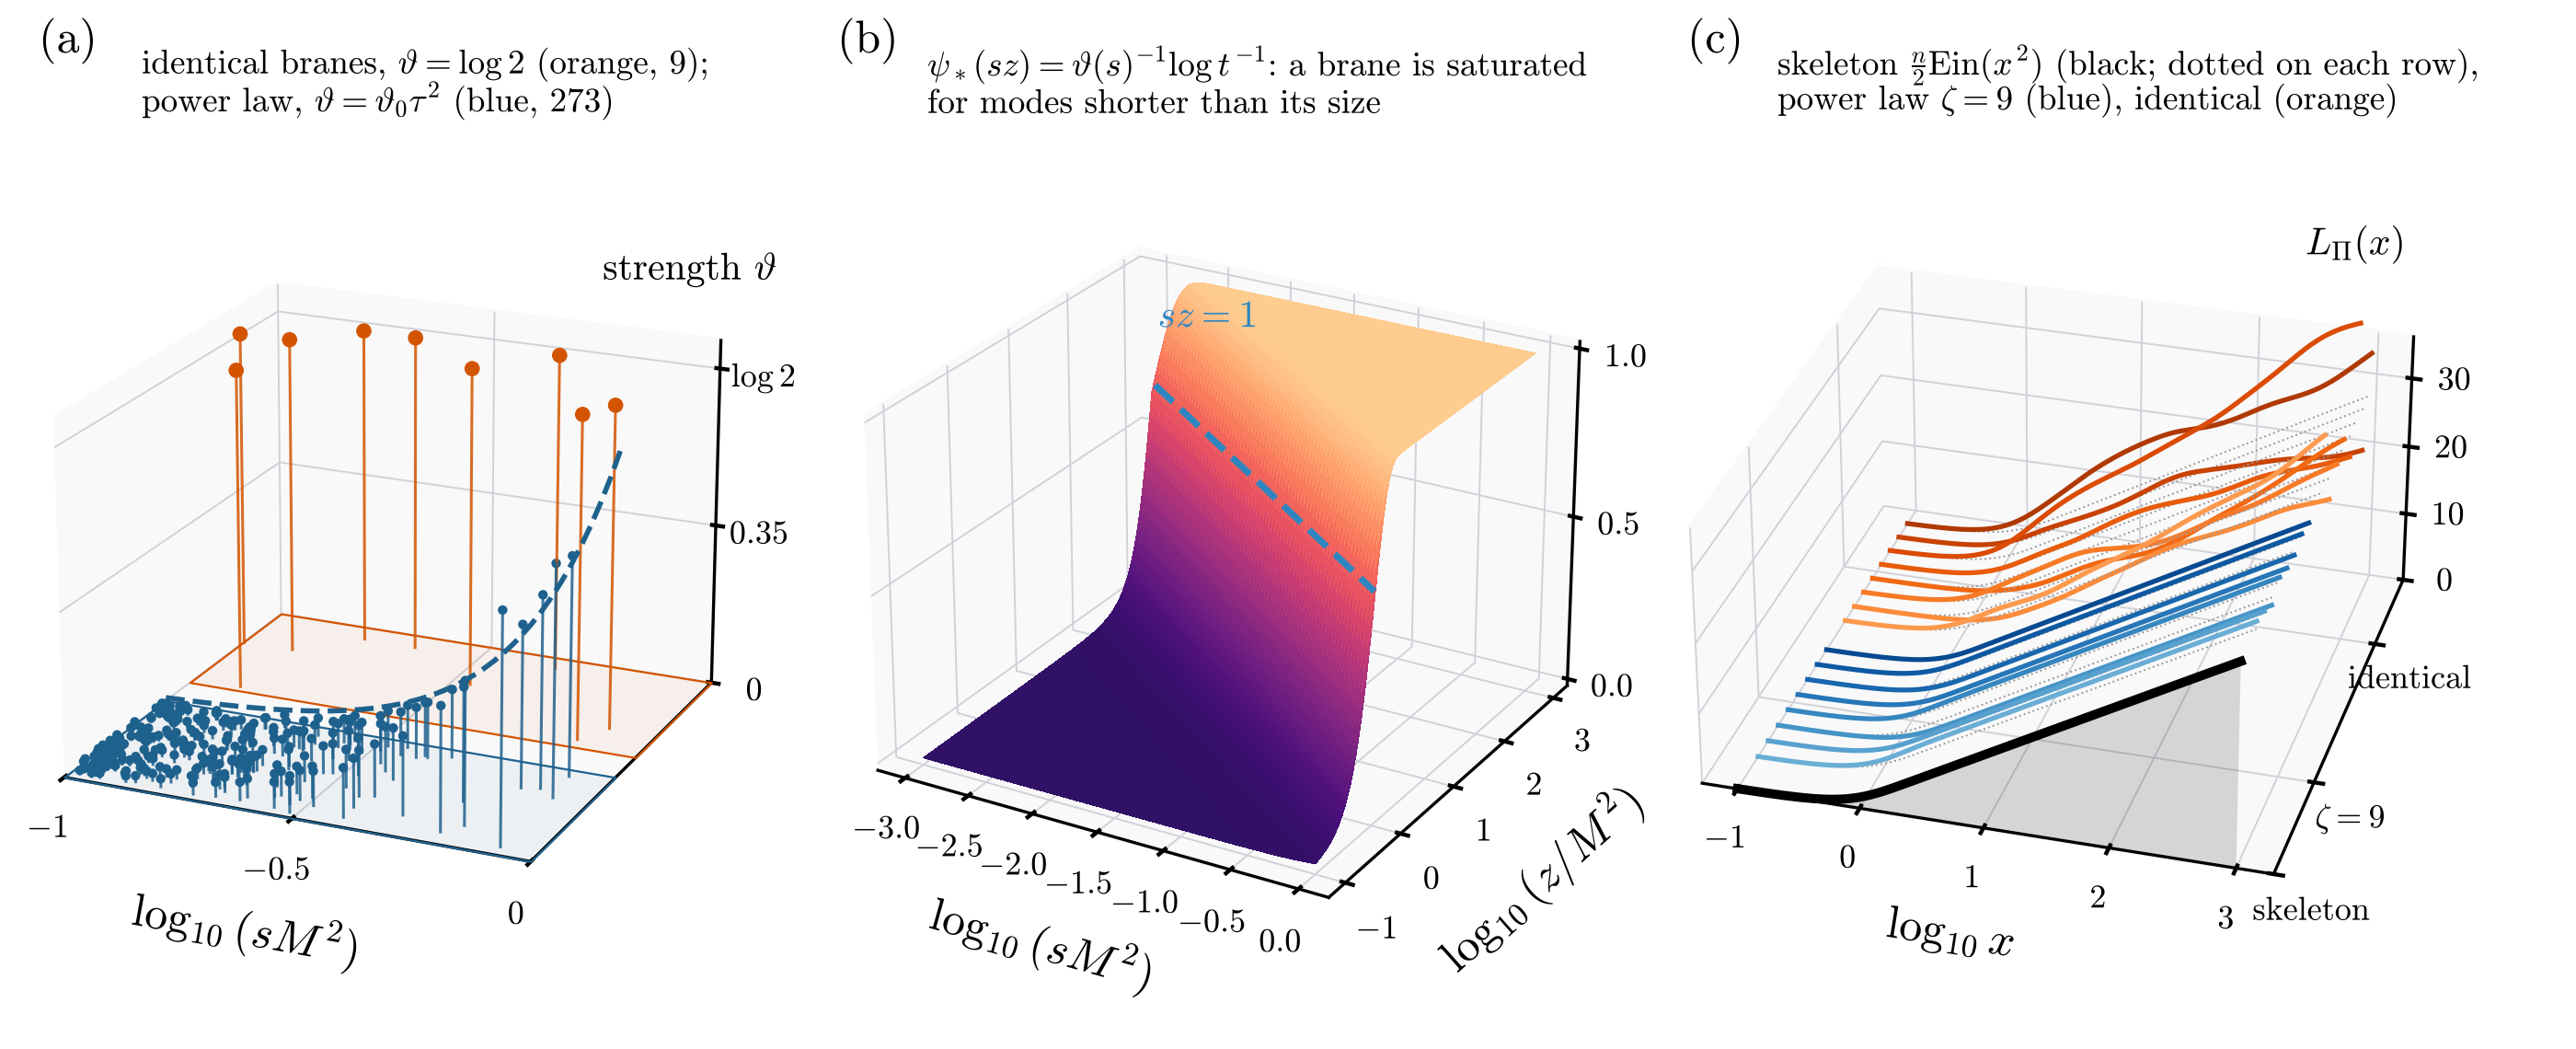
\includegraphics[width=\textwidth]{figs/fig_gas.png}
\caption{Two gases with the same strength per $e$-fold. (a) One realization of each, for $n=4$ and sizes between $0.1\,M^{-2}$ and $M^{-2}$: identical branes with $\vartheta_0=\log2$ (orange) and the fine-grained power law~\eqref{eq:finegrain} with $\zeta=2$ (blue). Each brane is a stem at its size, at a random transverse position, with height equal to its strength. At the smallest sizes the fine-grained gas has $100$ times more branes per $e$-fold, each $100$ times weaker. The dashed curve is the strength $\vartheta_0\tau^2$ of the power law. The value $\zeta=2$ keeps the number of stems small enough to draw; condition (G) needs $\zeta>4$. (b) The exponent of the single-brane factor in units of the strength of the brane, $\psi_*(sz)=\vartheta(s)^{-1}\log t^{-1}$, over the plane of $\log s$ and $\log z$. It switches on across the line $sz=1$ (dashed), so at fixed $z$ the exponent $L_\Pi$ of Eq.~\eqref{eq:aPi} collects the strength of the branes larger than $1/z$, which is the origin of the power law~\eqref{eq:a-asym}. (c) The exponent $L_\Pi(x)$ along the Euclidean axis for eight realizations of each gas, identical branes and the power law with $\zeta=9$, drawn as a waterfall against the skeleton $n\Phi(x)=\frac n2\Ein(x^2)$ (thick, in front, and dotted on each row). The fine-grained realizations run parallel to the skeleton at large $x$, offset by $R_\infty$; the realizations of identical branes drift away from it like random walks in $\log x$ (Sec.~\ref{sec:fluct}). For $\zeta=9$ the branes smaller than $0.3\,M^{-2}$ are represented by the Gaussian limit of their compensated strength, as in Fig.~\ref{fig:fluct}.}
\label{fig:gas}
\end{figure*}

\subsection{The skeleton in closed form}
\label{sec:closed}

For the response~\eqref{eq:phistar} everything about the skeleton can be written in closed form. The substitution $u=w^2\tau^2$ in Eq.~\eqref{eq:Phi} gives
\begin{equation}
\Phi(w)=\frac12\int_0^{w^2}\frac{1-e^{-u}}{u}\,\dd u=\frac12\Ein(w^2),
\end{equation}
so that $\hat a$ is the function of Eq.~\eqref{eq:a-intro}. The entire function $\Ein$ has the series $\Ein(w)=\sum_{k\ge1}(-1)^{k+1}w^k/(k\,k!)$, and we need three facts about it and about the exponential integral $E_1(y)=\int_y^\infty e^{-t}\,\dd t/t$~\cite{DLMF}.

First, Euler's constant is
\begin{equation}
\label{eq:gamma-id}
\gE=\int_0^1\frac{1-e^{-t}}{t}\,\dd t-\int_1^\infty\frac{e^{-t}}{t}\,\dd t .
\end{equation}
To see this, start from $\Gamma'(1)=-\gE$, that is $-\gE=\int_0^\infty e^{-t}\log t\,\dd t$, and integrate by parts on each half of the range: on $[0,1]$ with the antiderivative $1-e^{-t}$ of $e^{-t}$, so that the boundary term $(1-e^{-t})\log t$ vanishes at both ends, and on $[1,\infty)$ with $-e^{-t}$, so that the boundary term vanishes at $t=1$ and at infinity. The two pieces are $-\int_0^1(1-e^{-t})\,\dd t/t$ and $\int_1^\infty e^{-t}\,\dd t/t$, and their sum is $-\gE$.

Second, for $y>0$,
\begin{equation}
\label{eq:Ein-E1}
\Ein(y)=\log y+\gE+E_1(y),\qquad 0<E_1(y)\le\frac{e^{-y}}{y}.
\end{equation}
Split $\Ein(y)=\int_0^1(1-e^{-t})\,\dd t/t+\int_1^y\dd t/t-\int_1^ye^{-t}\,\dd t/t$ and complete the last integral to $\int_1^\infty$; by Eq.~\eqref{eq:gamma-id} the constants combine into $\gE$, and what is left is $\log y+E_1(y)$. The bound follows from $1/t\le1/y$ on $[y,\infty)$. Both sides of the identity are analytic in the plane cut along the negative axis, so it continues to $|\arg y|<\pi$ with principal branches. For $\mathrm{Re}\,y>0$ the integral along the horizontal ray from $y$ gives $|E_1(y)|\le e^{-\mathrm{Re}\,y}\int_0^\infty e^{-u}\,\dd u/|y+u|\le e^{-\mathrm{Re}\,y}/|y|$, since $|y+u|\ge|y|$ for $u\ge0$.

Third, the function $g(y)=\Ein(y)-\log(1+y)$ is nondecreasing on $[0,\infty)$, with $g(0)=0$ and $g(\infty)=\gE$. Indeed
\[
g'(y)=\frac{1-e^{-y}}{y}-\frac1{1+y}=\frac{1-(1+y)e^{-y}}{y(1+y)}\ge0,
\]
because $e^{y}\ge1+y$, and by Eq.~\eqref{eq:Ein-E1} $g(y)=\gE+E_1(y)-\log(1+y^{-1})\to\gE$.

These three facts give the properties of the skeleton. They are collected in Table~\ref{tab:a} and plotted in Figs.~\ref{fig:formfactor} and~\ref{fig:complex}; we now derive them one by one. Section~\ref{sec:fluct} carries each of them over to a realization.

\textit{Two-sided bound.} Putting $y=x^2$ in the third fact, for every real $z$,
\begin{equation}
\label{eq:twosided}
\bigl(1+x^2\bigr)^{n/2}\le\hat a(z)\le\hat c\,\bigl(1+x^2\bigr)^{n/2},\qquad\hat c=e^{n\gE/2}.
\end{equation}
The skeleton is pinched between two polynomials of degree $2n$ in $x$ on the whole real axis, although it has no zero anywhere.

\textit{Large momenta on the real axis.} For $|x|\ge1$, Eq.~\eqref{eq:Ein-E1} gives $\hat a(z)=\hat c\,|x|^{n}\exp[\frac n2E_1(x^2)]$, so $\hat a-\hat c|x|^n$ is smaller than $\hat c|x|^n$ by a factor of order $e^{-x^2}/x^2$.

\textit{Small momenta.} From the series of $\Ein$,
\begin{equation}
\label{eq:IR}
\hat a(z)=1+\frac n2\,x^2+\frac{n(n-1)}8\,x^4+O(x^6),
\end{equation}
with no term linear in $x$, in line with $\psi_*'(0)=0$.

\textit{Derivatives.} Write $\hat a=e^{H}$ with $H(z)=\frac n2\Ein(z^2/M^4)$. Then
\[
H'(z)=\frac{n\bigl(1-e^{-x^2}\bigr)}{z},
\]
which is entire. For $|x|\ge1$ it equals $n/z$ minus a term whose derivatives of every order are bounded by $C_j\,e^{-x^2/2}M^{-2-2j}$, so $|H^{(j)}(z)|\le C_jM^{-2j}(1+|x|)^{-j}$ for $j\ge1$ on the real axis. By Fa\`a di Bruno's formula $\hat a^{(j)}$ is $\hat a$ times a polynomial in $H',\dots,H^{(j)}$ whose monomials all have total order $j$, so $|\hat a^{(j)}|\le C_jM^{-2j}(1+|x|)^{-j}\hat a$, and with Eq.~\eqref{eq:twosided}
\begin{equation}
\label{eq:aderiv}
\bigl|\hat a^{(j)}(z)\bigr|\le C_jM^{-2j}(1+|x|)^{n-j},\qquad z\in\bR .
\end{equation}

\textit{The nonlocal remainder.} The function
\begin{equation}
\label{eq:Ghat}
\hat{\mathcal G}(z)=\frac{\hat a(z)-1}{z}-\frac{\hat c\,z^{n-1}}{M^{2n}}
\end{equation}
is entire, because $\hat a-1$ vanishes at $z=0$. It measures how far the nonlocal part of the action would be from a polynomial if the skeleton were the form factor. On $[0,M^2]$ it is a smooth function on a compact interval, and for $z\ge M^2$,
\[
\hat{\mathcal G}(z)=-\frac1z+\frac{\hat c\,x^n}{z}\Bigl(e^{\frac n2E_1(x^2)}-1\Bigr).
\]
Since $E_1$ and its derivatives at $y=x^2$ are bounded by polynomials in $1/x$ times $e^{-x^2}$, the second term and all its derivatives are exponentially small, and the derivatives of $-1/z$ give
\begin{equation}
\label{eq:Ghatsymbol}
\bigl|\hat{\mathcal G}^{(j)}(z)\bigr|\le C_jM^{-2-2j}(1+x)^{-1-j},\qquad z\ge0 .
\end{equation}
In the language of pseudodifferential operators $\hat{\mathcal G}$ is a symbol of order $-1$. In the same way $\hat a-\hat c\,x^n=\hat c\,x^n(e^{\frac n2E_1(x^2)}-1)$ for $x\ge1$, so $|\frac{\dd^j}{\dd z^j}(\hat a-\hat cx^n)|\le C_jM^{-2j}(1+x)^{-j}$ on $[0,\infty)$: a symbol of order $0$. Figure~\ref{fig:formfactor}(c) shows $z\,\hat{\mathcal G}(z)$, which tends to $-1$.

\textit{Complex momenta.} Let $S_\delta=\{z:|\arg z|\le\pi/4-\delta\}$ with $0<\delta<\pi/4$. For $z\in S_\delta$ we have $\mathrm{Re}\,z^2\ge|z|^2\sin2\delta>0$, and the continued identity~\eqref{eq:Ein-E1} with its bound gives
\begin{equation}
\label{eq:cone}
\begin{gathered}
\hat a(z)=\hat c\Bigl(\frac z{M^2}\Bigr)^{\!n}\Bigl[1+\epsilon(z)\Bigr],\\
|\epsilon(z)|\le\exp\Bigl(\frac{nM^4e^{-|z|^2\sin2\delta/M^4}}{2|z|^2}\Bigr)-1 .
\end{gathered}
\end{equation}
Because $\hat a(-z)=\hat a(z)$, the same holds in the reflected cone around the negative axis. Inside the two cones $|\arg(\pm z)|<\pi/4$, which contain the Euclidean and the Lorentzian axes, the skeleton is a monomial up to corrections that fall like a Gaussian. Outside them it is not polynomially bounded. On the imaginary axis $\hat a(iy)=\exp[-\frac n2\int_0^{y^2/M^4}(e^{t}-1)\,\dd t/t]$ falls faster than any exponential of $y^2$, and in between $|\hat a|$ oscillates with growing amplitude (Fig.~\ref{fig:complex}). This rules out a naive Wick rotation, and Sec.~\ref{sec:unitarity} explains how the theory is defined instead.

\begin{figure*}[t]
\centering
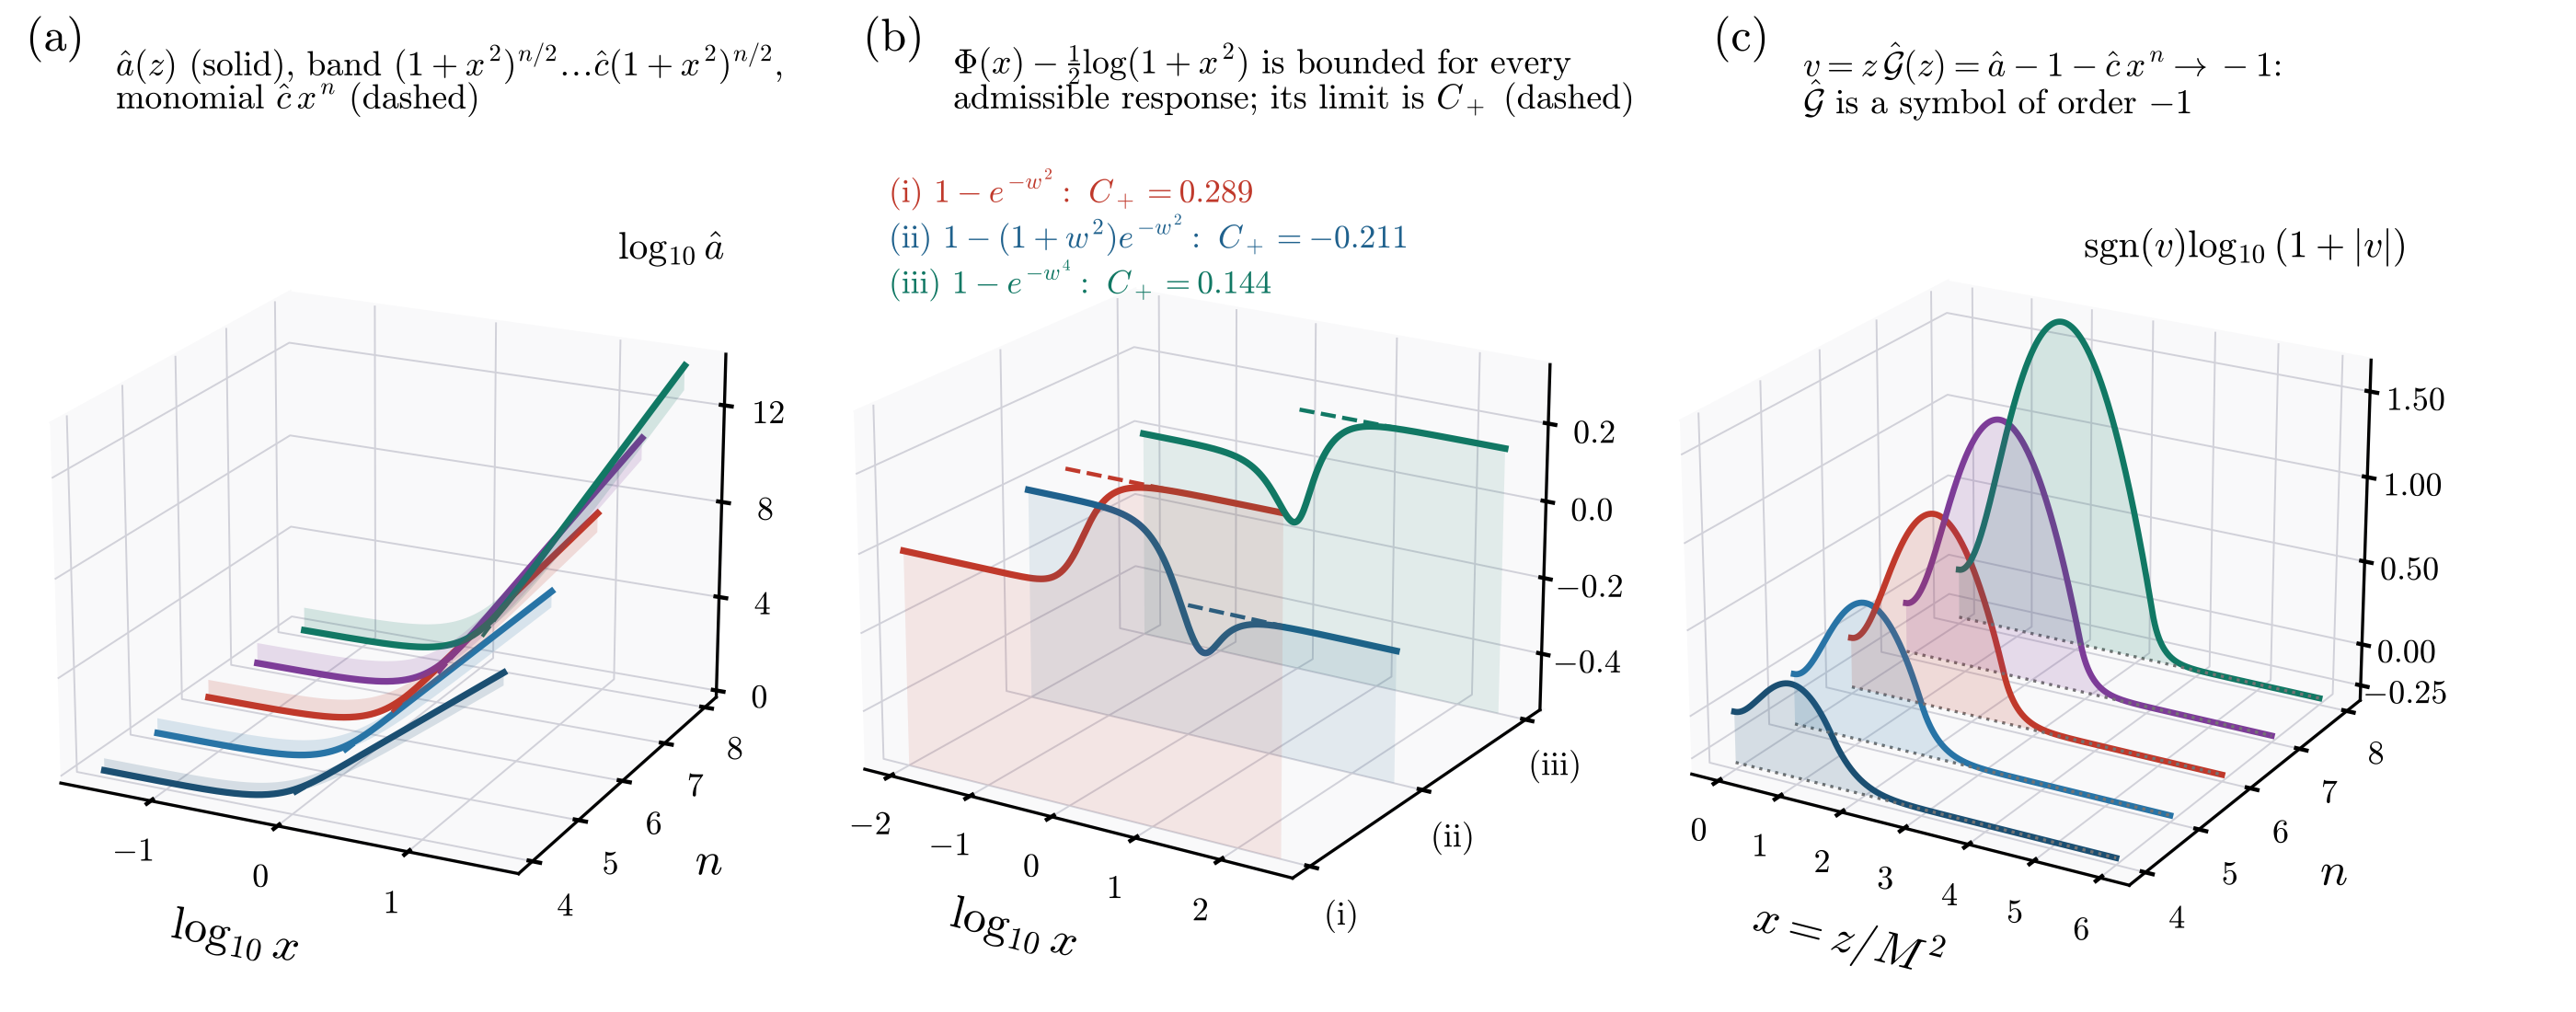
\includegraphics[width=\textwidth]{figs/fig_formfactor.png}
\caption{The skeleton on the real axis. (a) $\log_{10}\hat a(z)$ for $n=4,\dots,8$ (solid) inside the band of the two-sided bound~\eqref{eq:twosided}, $(1+x^2)^{n/2}\le\hat a\le\hat c\,(1+x^2)^{n/2}$ (shaded), with the monomial $\hat c\,x^n$ that $\hat a$ approaches at large $x$ (dashed). (b) $\Phi(x)-\frac12\log(1+x^2)$ for the three admissible responses of Table~\ref{tab:class}: it is bounded for each of them, as Eq.~\eqref{eq:twosided-gen} states, and tends to the constant $C_+$ (dashed) of Eq.~\eqref{eq:cone-gen}. (c) $v=z\,\hat{\mathcal G}(z)=\hat a-1-\hat c\,x^n$ for $n=4,\dots,8$, plotted as $\sgn(v)\log_{10}(1+|v|)$: it is bounded and tends to $-1$ (dotted), so the nonlocal remainder~\eqref{eq:Ghat} is a symbol of order $-1$ for every $n$.}
\label{fig:formfactor}
\end{figure*}

\begin{figure*}[t]
\centering
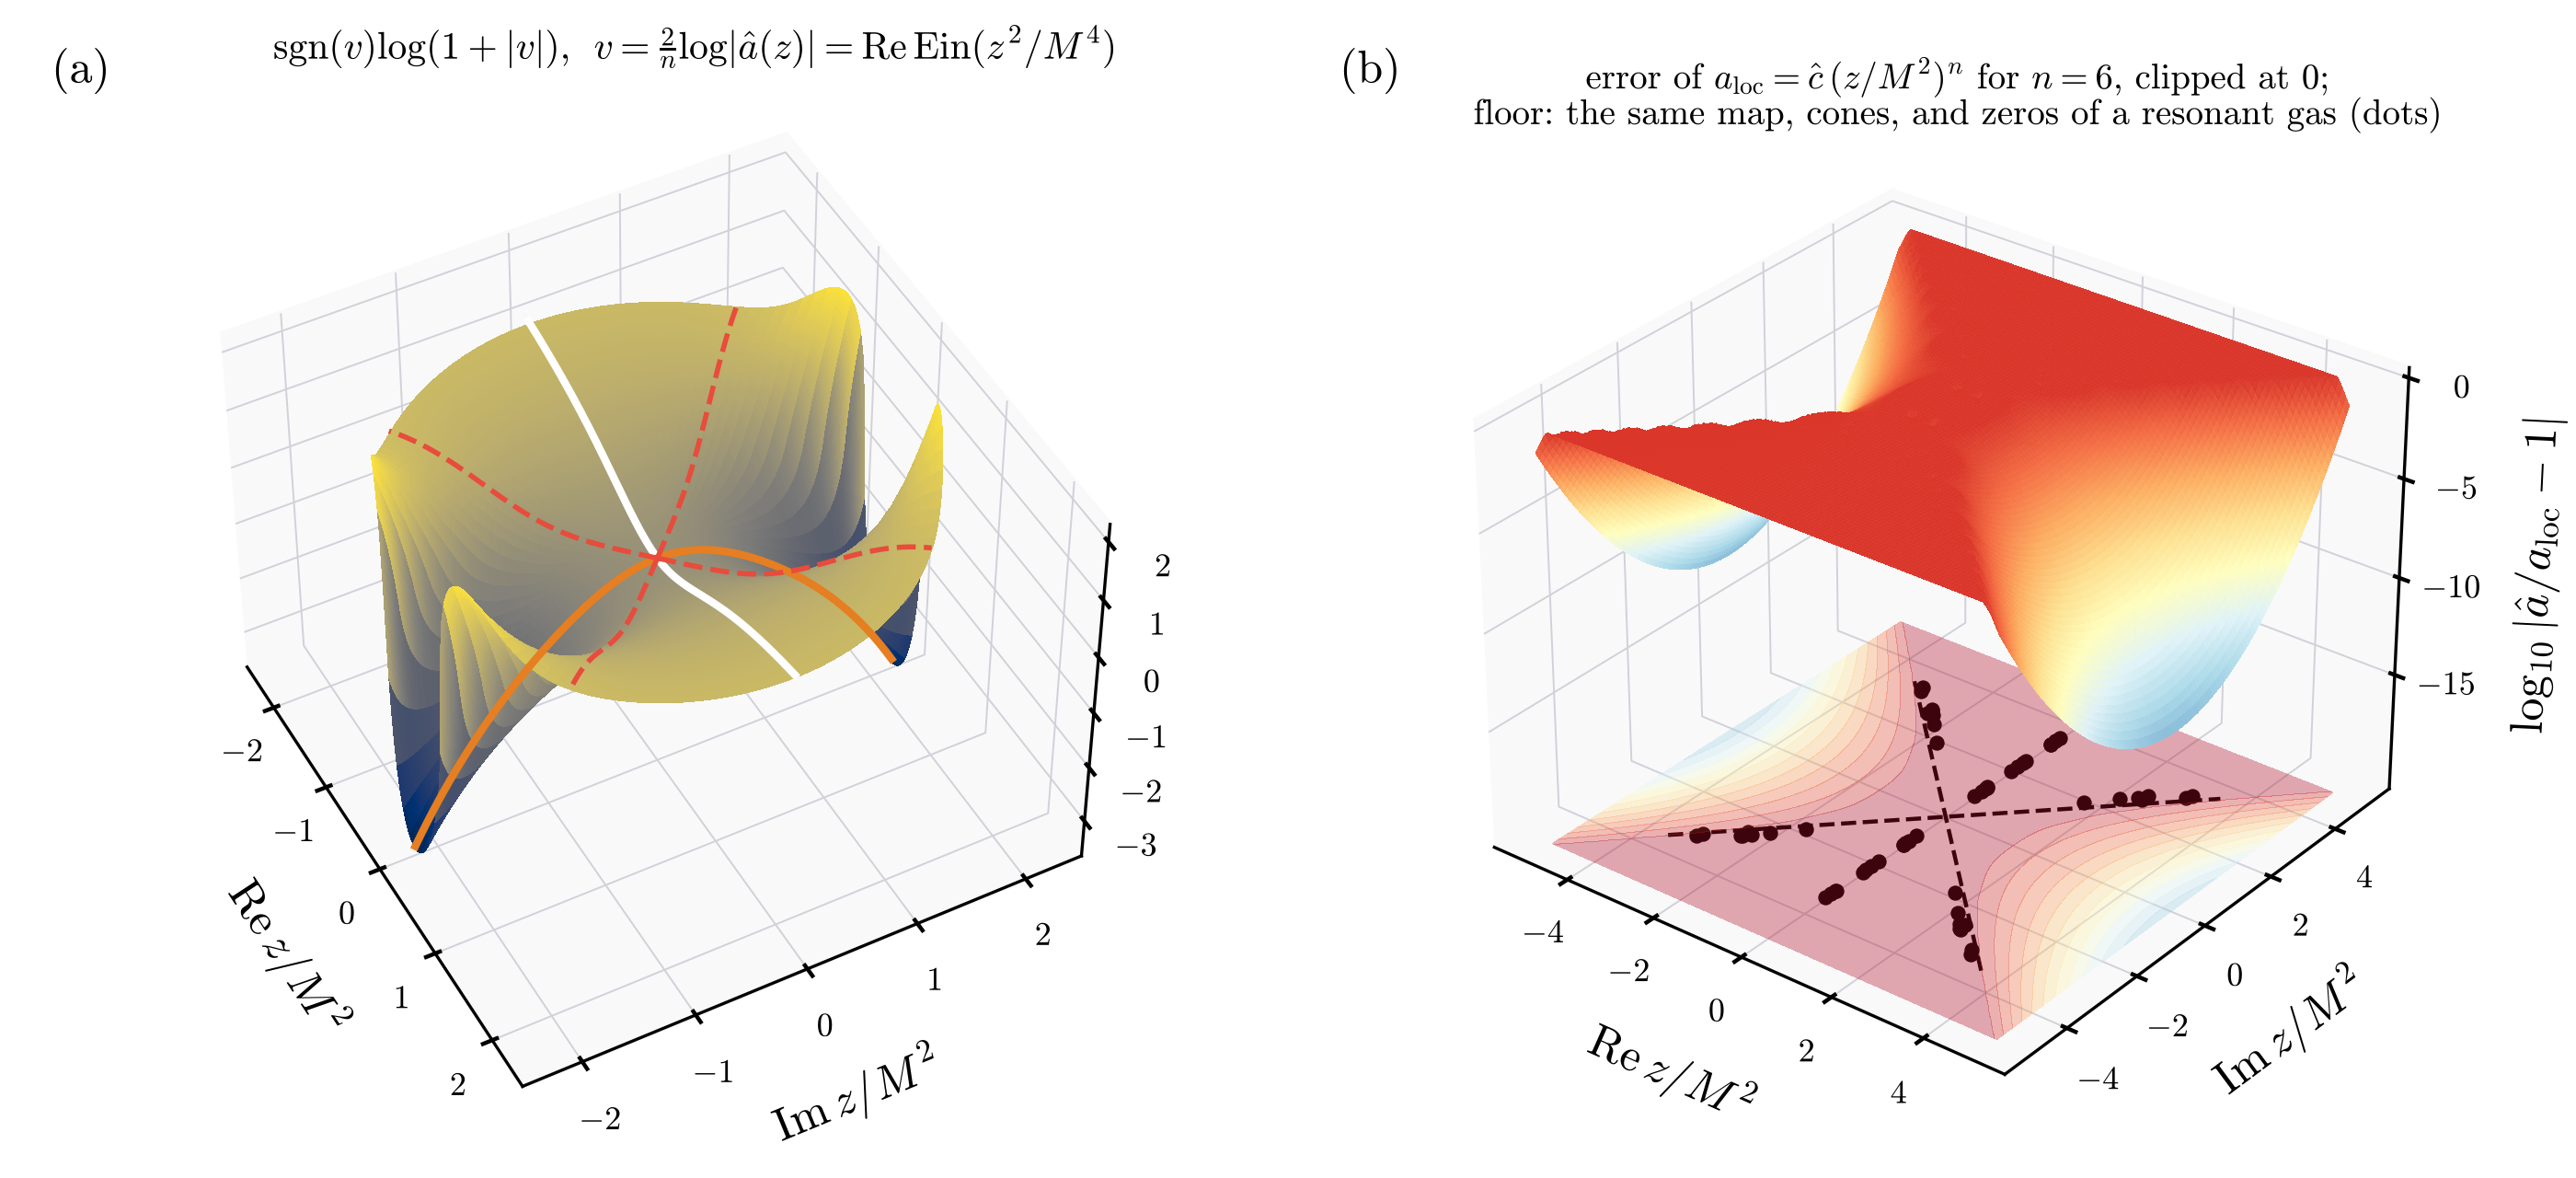
\includegraphics[width=\textwidth]{figs/fig_complex.png}
\caption{The skeleton in the complex $z$ plane. (a) $v=\frac2n\log|\hat a|=\mathrm{Re}\,\Ein(z^2/M^4)$ over the disk $|z|\le2.2M^2$, plotted as $\sgn(v)\log(1+|v|)$ to compress its range. Along the real axis (white) it rises like $2\log|z|$; along the imaginary axis (orange) it falls without bound; the dashed red lines are the cone boundaries $\arg z=\pm\pi/4,\pm3\pi/4$, between which $|\hat a|$ oscillates. (b) Accuracy of the local approximation $\hat c\,(z/M^2)^n$ for $n=6$, $\log_{10}|\hat a/(\hat cz^n/M^{2n})-1|$ clipped at $0$: the error is exponentially small inside the cones $|\arg(\pm z)|<\pi/4$ (blue), Eq.~\eqref{eq:cone}, and of order one outside. The floor repeats the map as a contour plot, with the cone boundaries (dashed) and, as black dots, the zeros that a frozen gas of the resonant factors $2-e^{-s^2z^2}$ of Eq.~\eqref{eq:qzeros} would have for sizes in $[0.15,1]\,M^{-2}$. They all lie outside the cones. A gas of branes obeying (S5) has none.}
\label{fig:complex}
\end{figure*}

\subsection{Other passive responses}
\label{sec:class}

The closed forms of Sec.~\ref{sec:closed} rest on the choice $\psi=\psi_*$, but the field theory of Secs.~\ref{sec:action}--\ref{sec:unitarity} does not. We call a response \emph{admissible} if its exponent satisfies (S1)--(S4), and show that every admissible response gives a skeleton with the properties used there. Only two numbers change from one response to another, the constant $C_+$ of Eq.~\eqref{eq:Phi-asym} and the moment $\mu_\psi=\int_0^\infty t\,(1-\psi(t))\,\dd t$.

\textit{Analyticity and the real axis.} Section~\ref{sec:formfactor} already shows that $\hat a=e^{n\Phi}$ is entire, has no zeros and satisfies $\hat a(0)=1$; its Taylor coefficients are real. By (S2), $\Phi(x)=\int_0^1\psi(x\tau)\,\dd\tau/\tau\ge0$ for real $x$ of either sign, so $\hat a\ge1$ on the whole real axis. The function $\Phi(x)-\frac12\log(1+x^2)$ is continuous on $\bR$ and tends to $C_\pm$ as $x\to\pm\infty$, by Eq.~\eqref{eq:Phi-asym}, so it is bounded, between $m_\psi$ and $M_\psi$ say, and
\begin{equation}
\label{eq:twosided-gen}
e^{nm_\psi}\bigl(1+x^2\bigr)^{n/2}\le\hat a(z)\le e^{nM_\psi}\bigl(1+x^2\bigr)^{n/2},\qquad z\in\bR .
\end{equation}
For $\psi_*$ this is Eq.~\eqref{eq:twosided}, with $m_\psi=0$ and $M_\psi=\gE/2$.

\textit{Symbols.} With $H=n\Phi(z/M^2)$ we have $H'(z)=n\psi(x)/z$, and for $|x|\ge1$ this is $n/z$ minus $n(1-\psi(x))/z$, whose derivatives decay faster than any power by (S3). The argument of Sec.~\ref{sec:closed} then gives Eq.~\eqref{eq:aderiv} with the constant $e^{nM_\psi}$. Put $\hat c=e^{nC_+}$. For $x\ge1$, $\hat a-\hat c\,x^n=\hat c\,x^n(e^{n\rho_+(x)}-1)$, and $\rho_+$ and all its derivatives decay faster than any power, so $\hat a-\hat cx^n$ is a symbol of order $0$ and $\hat{\mathcal G}$ is a symbol of order $-1$: Eq.~\eqref{eq:Ghatsymbol} holds as it stands.

\textit{Cones.} Let $z=re^{i\alpha}$ with $|\alpha|\le\theta-\delta$. The function $g(w)=\Phi(w)-\log w$ is analytic in the sector and $g'(w)=-(1-\psi(w))/w$, which by (S4) is bounded by $C_N|w|^{-N-1}$ for every $N$. The integral of $g'$ along the ray from $z$ to infinity therefore converges and is $O(r^{-N})$, so $g(z)$ tends to a limit $L(\alpha)$ along each ray, with an error $O(r^{-N})$. The limit does not depend on $\alpha$, because the integral of $g'$ over an arc of radius $t$ between two rays is at most $\pi t\cdot C_Nt^{-N-1}\to0$. On the positive axis $L(0)=C_+$ by Eq.~\eqref{eq:Phi-asym}. Hence, in the sector,
\begin{equation}
\label{eq:cone-gen}
\hat a(z)=\hat c\Bigl(\frac z{M^2}\Bigr)^{\!n}e^{n\rho(z)},\qquad|\rho(z)|\le C_{N,\delta}\Bigl|\frac{M^2}z\Bigr|^N ,
\end{equation}
for every $N$, with $\hat c=e^{nC_+}$, and the same holds around the negative axis with $C_-$ and $(-z/M^2)^n$. For $\psi_*$ this is Eq.~\eqref{eq:cone}, where the remainder is even Gaussian.

\textit{The zero-point moment.} Section~\ref{sec:vacuum} needs the integral of $\Phi(k^2/M^2)$ over four-momentum in dimensional regularization. Its Mellin transform is elementary. For $-2<\mathrm{Re}\,s<0$, exchanging the order of integration in Eq.~\eqref{eq:Phi} gives $\int_0^\infty w^{s-1}\Phi(w)\,\dd w=-\tilde\psi(s)/s$, with $\tilde\psi(s)=\int_0^\infty u^{s-1}\psi(u)\,\dd u$; the strip is where both integrals converge, since $\psi(u)=O(u^2)$ at small $u$ by passivity and $\psi\to1$ at large $u$. Splitting $\tilde\psi$ at $u=1$ and writing $\psi=1-(1-\psi)$ on $[1,\infty)$ continues it to $\mathrm{Re}\,s>-2$, $s\ne0$, and for $\mathrm{Re}\,s>0$ the continuation is $\tilde\psi(s)=-\int_0^\infty u^{s-1}(1-\psi(u))\,\dd u$. At $s=D/2=2$,
\begin{equation}
\label{eq:moment}
\begin{gathered}
\int\frac{\dd^4k}{(2\pi)^4}\,\Phi\Bigl(\frac{k^2}{M^2}\Bigr)=\frac{M^4}{32\pi^2}\,\mu_\psi,\\
\mu_\psi=\int_0^\infty t\,\bigl(1-\psi(t)\bigr)\,\dd t ,
\end{gathered}
\end{equation}
which is positive and finite by (S2) and (S3).\footnote{For $\psi_*$, $\Phi(w)=\frac12\Ein(w^2)$ and $\mu_{\psi_*}=\int_0^\infty te^{-t^2}\dd t=\frac12$, so the right side is $M^4/(64\pi^2)$. This agrees with Sec.~\ref{sec:vacuum}, where the same integral is done in the variable $k^4/M^4$ with the Mellin transform~\eqref{eq:mellin}.} For a single brane of size $\tau/M^2$ no continuation is needed, because the integrand falls off rapidly by (S3) and the integral converges absolutely:
\begin{equation}
\label{eq:moment1}
\int\frac{\dd^4k}{(2\pi)^4}\Bigl[\psi\Bigl(\frac{\tau k^2}{M^2}\Bigr)-1\Bigr]=-\frac{M^4}{16\pi^2\tau^2}\,\mu_\psi ,
\end{equation}
as follows from the substitution $u=\tau k^2/M^2$, after which the angular integration leaves $\dd^4k/(2\pi)^4\to u\,\dd u\,M^4/(16\pi^2\tau^2)$.

\textit{Small momenta.} Passivity gives $\psi(w)=\psi_2w^2+O(w^3)$ with $\psi_2\ge0$, so $\hat a=1+\frac n2\psi_2x^2+O(x^3)$. The leading correction to the kinetic operator is of fourth order in momentum, as in Eq.~\eqref{eq:IR}.

Table~\ref{tab:class} gives three admissible responses and two that fail, and Fig.~\ref{fig:class} shows the sectors of (S4).

\begin{table*}[t]
\caption{Single-brane responses, given by the exponent $\psi$ of Eq.~\eqref{eq:onebrane}. The first three are admissible; for them $\hat c=e^{nC_+}$ is the leading coefficient of the skeleton, $\hat a\simeq\hat c\,x^n$, $\mu_\psi$ is the moment of Eq.~\eqref{eq:moment}, which fixes the mean zero-point energy~\eqref{eq:rho-gen}, and $\theta$ is the opening of the sectors of (S4). The last two violate the conditions named in the third column. Values of $\hat c$ are for $n=4$; for general $n$, $\hat c=e^{nC_+}$. Only the first row arises from the cell model of Sec.~\ref{sec:cells}: in the second and third, $1-\psi$ is not a characteristic function.}
\label{tab:class}
\begin{ruledtabular}
\setlength{\tabcolsep}{3pt}
\begin{tabular}{L{2.6cm}L{1.75cm}L{2.25cm}L{1.55cm}L{1.45cm}L{2.0cm}L{1.0cm}L{2.95cm}}
exponent $\psi(w)$ & small $w$ & $C_+$ & $\hat c$, $n=4$ & $\mu_\psi$ & $\rho_1/(nM^4)$ & $\theta$ & skeleton exponent $\Phi(x)$\\
\colrule
$1-e^{-w^2}$ & $w^2$ & $\gE/2=0.2886$ & $3.172$ & $\frac12$ & $3/(64\pi^2)$ & $\pi/4$ & $\frac12\Ein(x^2)$\\
$1-(1+w^2)e^{-w^2}$ & $\frac12w^4$ & $(\gE-1)/2=-0.2114$ & $0.4293$ & $1$ & $3/(32\pi^2)$ & $\pi/4$ & $\frac12[\Ein(x^2)-1+e^{-x^2}]$\\
$1-e^{-w^4}$ & $w^4$ & $\gE/4=0.1443$ & $1.781$ & $\frac{\sqrt\pi}4$ & $3\sqrt\pi/(128\pi^2)$ & $\pi/8$ & $\frac14\Ein(x^4)$\\
\colrule
$1-e^{-w}$ & $w$ & \multicolumn{6}{L{11.4cm}}{fails (S2): unbounded below on the negative axis; the factor decays faster than any power on the timelike axis}\\
$w^2/(1+w^2)$ & $w^2$ & \multicolumn{6}{L{11.4cm}}{fails (S1) and (S3): poles at $w=\pm i$, and $1-\psi\sim w^{-2}$, so $G$ and $\Lambda$ run at one loop}\\
\end{tabular}
\end{ruledtabular}
\end{table*}

\begin{figure*}[t]
\centering
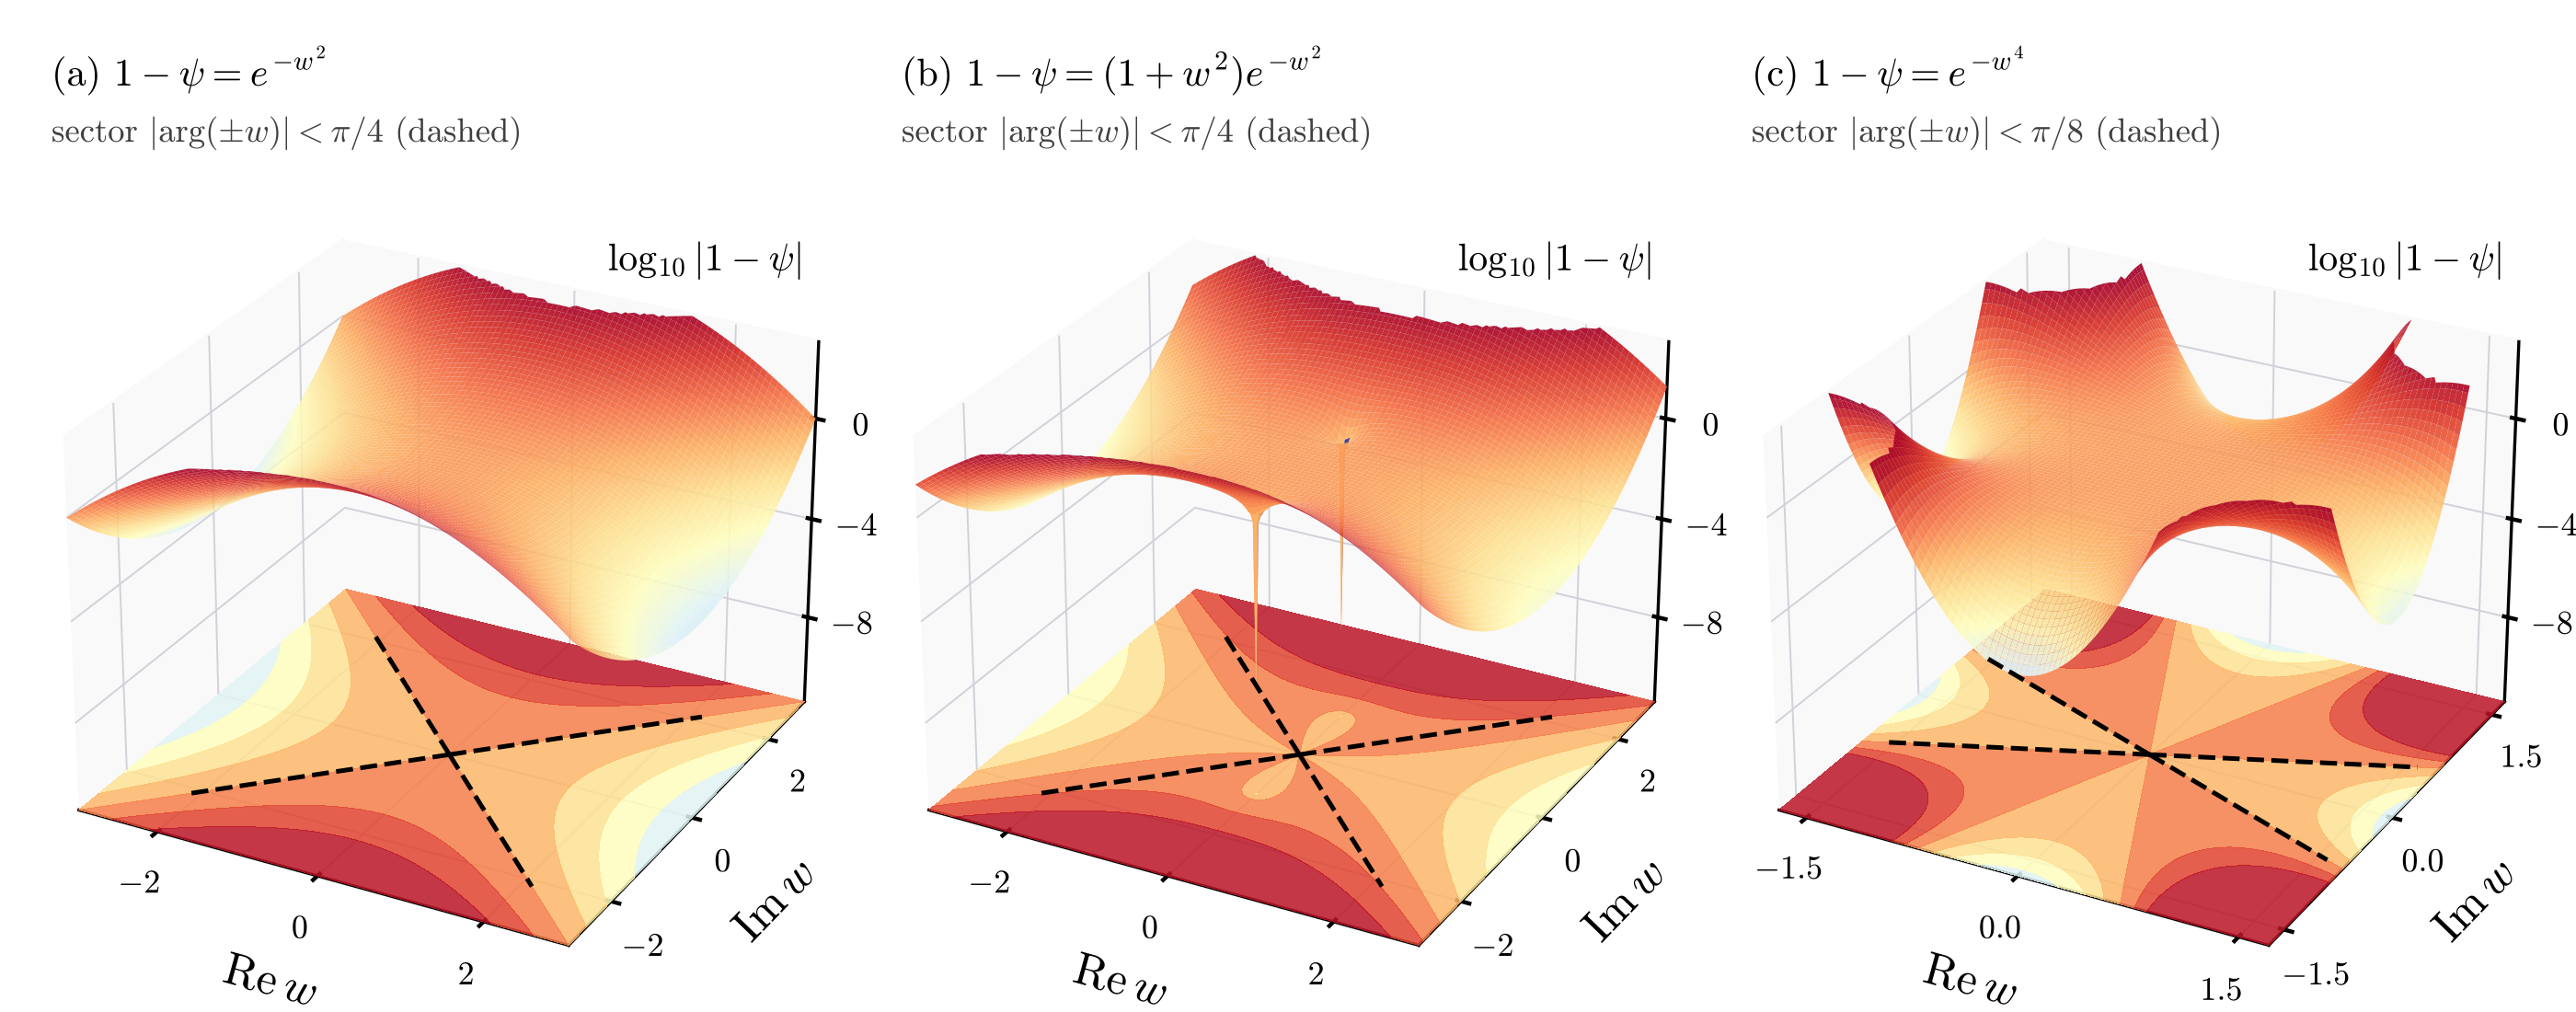
\includegraphics[width=\textwidth]{figs/fig_class.png}
\caption{The saturation sectors of condition (S4) for the three admissible exponents of Table~\ref{tab:class}. Each surface is $\log_{10}|1-\psi(w)|$ over the complex $w$ plane, clipped at $-8$ below and $+3$ above, with the floor showing the same quantity as a contour map. Where the surface is low the brane is saturated, $\psi\simeq1$; the dashed lines are the sector boundaries, $\arg w=\pm\pi/4$ in (a) and (b) and $\arg w=\pm\pi/8$ in (c). The exponent $1-e^{-w^4}$ of panel (c) is also saturated around the imaginary axis, which (S4) does not require.}
\label{fig:class}
\end{figure*}

\subsection{Fluctuations of a realization}
\label{sec:fluct}

The skeleton has every property that the field theory needs. We now show that, under (G), almost every realization has them too, with a random constant in place of $\hat c$. The two differ by the factor $e^{R_\Pi}$ of Eq.~\eqref{eq:split}, so everything rests on how $R_\Pi$ behaves at large $|z|$.

\textit{The limit at large momentum.} At large real $x$ every brane larger than $1/x$ is saturated and contributes its full strength. This suggests comparing $R_\Pi$ with the total strength of the gas measured from its mean,
\begin{equation}
\label{eq:Rinf}
\begin{aligned}
R_\infty&=\int\vartheta(s)\,(\Pi-\nu)(\dd s)\\
&=\lim_{\eta\to0}\Bigl[\sum_{s\in\Pi,\;s>\eta/M^2}\vartheta(s)-n\log\frac1\eta\Bigr].
\end{aligned}
\end{equation}
The sum in brackets has mean $\int_{\eta/M^2}^{1/M^2}\vartheta\,\dd\nu=n\log(1/\eta)$ by Eq.~\eqref{eq:intensity}, and by Eq.~\eqref{eq:isometry} its fluctuation has variance $n[V(1)-V(\eta)]$. Under (G) $V(1)$ is finite, and Sec.~\ref{sec:avg} gives the limit almost surely, with
\begin{equation}
\label{eq:Rinfstats}
\bE R_\infty=0,\qquad\bE R_\infty^2=nV(1).
\end{equation}
The difference
\begin{equation}
\label{eq:fdef}
R_\Pi(z)-R_\infty=\int\vartheta(s)\bigl[\psi(sz)-1\bigr]\,(\Pi-\nu)(\dd s)
\end{equation}
is carried by the branes that are not saturated at $z$.

\textit{Mean-square decay.} By Eq.~\eqref{eq:isometry}, for complex $z$ and $w=z/M^2$,
\begin{equation}
\label{eq:msq}
\bE\bigl|R_\Pi(z)-R_\infty\bigr|^2=n\int_0^1\vartheta(\tau)\,\bigl|1-\psi(w\tau)\bigr|^2\,\frac{\dd\tau}\tau .
\end{equation}
Let $|w|\ge1$ and $|\arg(\pm w)|\le\theta-\delta$. For $\tau\le1/|w|$ the point $w\tau$ lies in the closed unit disk, where $|1-\psi|\le B$, and this part of the integral is at most $nB^2V(1/|w|)\le nB^2C|w|^{-\sigma}$ by (G). For $\tau>1/|w|$ condition (S4) gives $|1-\psi(w\tau)|\le C_N|w\tau|^{-N}$. Choose $2N>\sigma$ and integrate by parts in $\int_{1/|w|}^1\tau^{-2N}\,\dd V(\tau)$: the boundary term at $\tau=1/|w|$ is negative, the one at $\tau=1$ is $V(1)$, and the remaining integral is $2N\int\tau^{-2N-1}V(\tau)\,\dd\tau\le2NC|w|^{2N-\sigma}/(2N-\sigma)$. Multiplying by $C_N^2|w|^{-2N}$, this part is also $O(|w|^{-\sigma})$, and
\begin{equation}
\label{eq:msdecay}
\begin{gathered}
\bE\bigl|R_\Pi(z)-R_\infty\bigr|^2\le K_\delta\Bigl|\frac{M^2}z\Bigr|^{\sigma},\\
|z|\ge M^2,\quad|\arg(\pm z)|\le\theta-\delta .
\end{gathered}
\end{equation}

\textit{Almost-sure decay.} Equation~\eqref{eq:msdecay} controls one point at a time. To control a whole sector we use the subharmonicity of $|f|^2$ for analytic $f$: $|f(w)|^2$ is at most the mean of $|f|^2$ over any disk centered at $w$ on which $f$ is analytic. Put $f(w)=R_\Pi(M^2w)-R_\infty$, an entire function, fix $\delta$, and let $A_k$ be the part of the sector $|\arg w|\le\theta-\delta$ with $2^k\le|w|\le2^{k+1}$, $k\ge1$. A disk of radius $r_k=2^{k-1}\sin(\delta/2)$ around a point of $A_k$ lies in the region $A'_k$ where $|\arg w|\le\theta-\delta/2$ and $2^{k-1}\le|w|\le2^{k+2}$. Hence
\[
\sup_{A_k}|f|^2\le\frac1{\pi r_k^2}\int_{A'_k}|f|^2\,\dd A ,
\]
and taking expectations with Eq.~\eqref{eq:msdecay} in the wider sector,
\[
\bE\sup_{A_k}|f|^2\le\frac{\operatorname{area}(A'_k)}{\pi r_k^2}\,K_{\delta/2}\,2^{-(k-1)\sigma}\le K'\,2^{-k\sigma},
\]
since the ratio of the area of $A'_k$ to $r_k^2$ does not depend on $k$. Chebyshev's inequality gives $\mathrm P\bigl(\sup_{A_k}|f|>2^{-k(\sigma/2-\varepsilon)}\bigr)\le K'2^{-2k\varepsilon}$, which is summable in $k$ for every $\varepsilon>0$. By the Borel--Cantelli lemma, almost surely $\sup_{A_k}|f|\le2^{-k(\sigma/2-\varepsilon)}$ for all but finitely many $k$, and on the remaining annuli $f$ is bounded because it is continuous. Taking $\delta$ and $\varepsilon$ rational, and treating the sectors around the negative axis in the same way, we conclude that almost surely
\begin{equation}
\label{eq:asdecay}
\begin{gathered}
\bigl|R_\Pi(z)-R_\infty\bigr|\le C_\Pi\Bigl|\frac{M^2}z\Bigr|^{\sigma/2-\varepsilon},\\
|z|\ge M^2,\quad|\arg(\pm z)|\le\theta-\delta ,
\end{gathered}
\end{equation}
for every $\delta\in(0,\theta)$ and every $\varepsilon>0$, with $C_\Pi$ finite and depending on the realization, on $\delta$ and on $\varepsilon$. For the power law below $\sigma=\zeta$, and the exponent matches, up to $\varepsilon$, the decay of the standard deviation of $R_\Pi(z)-R_\infty$, which falls like $|z|^{-\zeta/2}$, Eq.~\eqref{eq:varf}.

\textit{The form factor of a realization.} With Eqs.~\eqref{eq:split} and \eqref{eq:cone-gen}, Eq.~\eqref{eq:asdecay} says that almost surely, in the same sectors,
\begin{equation}
\label{eq:cone-real}
\begin{gathered}
a_\Pi(z)=c_\Pi\Bigl(\frac{\pm z}{M^2}\Bigr)^{\!n}e^{\eta_\Pi(z)},\qquad c_\Pi=e^{nC_\pm+R_\infty},\\
|\eta_\Pi(z)|\le C'_\Pi\Bigl|\frac{M^2}z\Bigr|^{\sigma/2-\varepsilon}.
\end{gathered}
\end{equation}
A realization has the asymptotics of the skeleton, with a random coefficient. Cauchy's estimate on a disk of radius $\frac12|z|\sin(\delta/2)$ around $z$, which stays inside the wider sector, bounds the derivatives: $|\eta_\Pi^{(j)}(z)|\le C_j|z|^{-j}|M^2/z|^{\sigma/2-\varepsilon}$. On the real axis $R_\Pi$ is continuous and tends to $R_\infty$ at both ends, so $\|R_\Pi\|=\sup_{\bR}|R_\Pi|$ is finite, and Eq.~\eqref{eq:twosided-gen} gives
\begin{equation}
\label{eq:twosided-real}
e^{nm_\psi-\|R_\Pi\|}\bigl(1+x^2\bigr)^{n/2}\le a_\Pi(z)\le e^{nM_\psi+\|R_\Pi\|}\bigl(1+x^2\bigr)^{n/2}
\end{equation}
for every real $z$.

Now let $\sigma>4$, as (G) requires, fix $\varepsilon$ with $0<\varepsilon<\sigma/2-2$, and put
\begin{equation}
\label{eq:msigma}
m_\sigma=\max\bigl(0,\,n-\sigma/2+\varepsilon\bigr),\qquad 0\le m_\sigma<n-2 .
\end{equation}
Then for $|x|\ge1$
\[
a_\Pi(z)-c_\Pi|x|^n=c_\Pi|x|^n\bigl(e^{\eta_\Pi}-1\bigr)=O\bigl(|x|^{\,n-\sigma/2+\varepsilon}\bigr),
\]
and each derivative falls by one more power of $x$; so $a_\Pi-c_\Pi x^n$ is a symbol of order $m_\sigma$, and $a_\Pi$ obeys the derivative bounds~\eqref{eq:aderiv} of the skeleton. When $\sigma>2n$ one may take $m_\sigma=0$, and $a_\Pi-c_\Pi x^n$ stays bounded, as it does for the skeleton; for $4<\sigma\le2n$ it grows, but more slowly than $x^{n-2}$. The nonlocal remainder of the realization,
\begin{equation}
\label{eq:G}
\mathcal G(z)=\frac{a_\Pi(z)-1}{z}-\frac{c_\Pi\,z^{n-1}}{M^{2n}},
\end{equation}
is entire, equals $-1/z+c_\Pi x^n(e^{\eta_\Pi}-1)/z$ for $x\ge1$, and obeys
\begin{equation}
\label{eq:Gsymbol}
\bigl|\mathcal G^{(j)}(z)\bigr|\le C_jM^{-2-2j}(1+x)^{m_\sigma-1-j},\qquad z\ge0 ,
\end{equation}
almost surely; the same bounds hold with $|z|$ in place of $z$ in every closed subsector of the sectors of (S4). So $\mathcal G$ is a symbol of order $m_\sigma-1$; for the skeleton it is a symbol of order $-1$, with corrections that fall faster than any power. The field theory of Secs.~\ref{sec:power}--\ref{sec:unitarity} uses only that the order is below $n-3$, and this is where the exponent $4$ in (G) comes from. The fluctuation of the gas at momentum $p$ must fall faster than $p^{-4}$, so that the one-loop integrals of Secs.~\ref{sec:poles1} and \ref{sec:vacuum} converge; the growth that $a_\Pi-c_\Pi x^n$ may then have is absorbed by the vertex bound of Sec.~\ref{sec:vertex}.

\textit{Identical branes.} Without (G) the conclusion fails, and it fails for the most obvious gas. Let all branes have the same strength $\vartheta_0$, so that $\nu=(n/\vartheta_0)\,\dd s/s$. For real $x$ the sum $R_\Pi(x)$ is an ordinary compensated sum, and Eq.~\eqref{eq:pgfl} with $f=e^{iu\vartheta_0\psi}-1$ gives its characteristic function,
\[
\Bigl|\bE\,e^{iuR_\Pi(x)}\Bigr|=\exp\Bigl[\frac n{\vartheta_0}\int_0^x\bigl(\cos(u\vartheta_0\psi(t))-1\bigr)\frac{\dd t}t\Bigr].
\]
As $x\to\infty$ the integrand tends to $\cos(u\vartheta_0)-1$, which is negative unless $u\vartheta_0\in2\pi\mathbb Z$, and $\int\dd t/t$ diverges, so the right side tends to $0$ for all such $u$. If $R_\Pi(x)$ converged in distribution, its characteristic function would converge to a function continuous at $u=0$~\cite{Feller1971}; the limit here is $1$ at $u=0$ and $0$ around it. So $R_\Pi(x)$ has no limit in distribution, and a fortiori no limit almost surely: $a_\Pi(x)/x^n$ does not converge, and no constant $c$ makes $a_\Pi-c\,x^n$ a symbol of order $0$. For $c>0$ this would force $R_\Pi(x)$ to converge. For $c\le0$ it would force $a_\Pi(x)$ to stay bounded, hence $R_\Pi(x)\le C-n\log x$ for large $x$, so that only a bounded number of branes could have $sx$ above a fixed $t_0$ beyond which $\psi\ge\frac12$; their number is Poisson with mean $(n/\vartheta_0)\log(x/t_0)$, and the probability of that event tends to zero. The variance shows the mechanism,
\begin{equation}
\label{eq:Psistar}
\begin{aligned}
\bE R_\Pi(x)^2&=n\vartheta_0\Psi_*(x),\\
\Psi_*(x)&=\int_0^1\psi_*(x\tau)^2\,\frac{\dd\tau}\tau=\Ein(x^2)-\tfrac12\Ein(2x^2)\\
&=\log|x|+\tfrac12(\gE-\log2)+O\bigl(e^{-x^2}\bigr),
\end{aligned}
\end{equation}
from $(1-e^{-u})^2=2(1-e^{-u})-(1-e^{-2u})$, the substitution $u=x^2\tau^2$ and Eq.~\eqref{eq:Ein-E1}. The saturated strength performs a random walk in $\log x$, one step of size $\vartheta_0$ for each of the roughly $(n/\vartheta_0)\log x$ branes larger than $1/x$. Such a gas still gives an entire form factor without zeros, by (S5), and $\log a_\Pi(x)/\log x\to n$ almost surely by the strong law of large numbers. But the local split of Sec.~\ref{sec:local}, on which the one-loop analysis rests, does not exist for it.

\textit{Statistics of a realization.} For the power law~\eqref{eq:finegrain} and $\psi_*$ the moments on the real axis are incomplete gamma functions. With $\gamma(b,y)=\int_0^yt^{b-1}e^{-t}\dd t$ and $(1-e^{-u})^2=1-2e^{-u}+e^{-2u}$,
\begin{align}
\bE R_\Pi(x)^2&=n\vartheta_0\Bigl[\frac1\zeta-\frac{\gamma(\frac\zeta2,x^2)}{x^{\zeta}}+\frac{\gamma(\frac\zeta2,2x^2)}{2\,(2x^2)^{\zeta/2}}\Bigr],\label{eq:varR}\\
\bE\bigl|R_\Pi(x)-R_\infty\bigr|^2&=\frac{n\vartheta_0}{2}\,\frac{\gamma(\frac\zeta2,2x^2)}{(2x^2)^{\zeta/2}}\le\frac{n\vartheta_0\,\Gamma(\frac\zeta2)}{2\,(2x^2)^{\zeta/2}} ,\label{eq:varf}
\end{align}
and $\bE R_\infty^2=n\vartheta_0/\zeta$. The leading coefficient $c_\Pi=\hat c\,e^{R_\infty}$ has $\bE\log c_\Pi=\log\hat c$, and by Eq.~\eqref{eq:expmoment}, with the substitution $t=\vartheta_0\tau^\zeta$,
\begin{equation}
\label{eq:EeR}
\bE\,c_\Pi=\hat c\,\exp\Bigl[\frac n\zeta\int_0^{\vartheta_0}\frac{e^{t}-1-t}{t^2}\,\dd t\Bigr].
\end{equation}
The image of $\nu$ under $s\mapsto\vartheta(s)$ is $(n/\zeta)\,\dd t/t^2$ on $(0,\vartheta_0]$, so $R_\infty$ is a centered, totally skewed variable whose L\'evy measure is that of a stable law of index one, cut off at $\vartheta_0$. Its jumps are positive, and since $e^{-\lambda t}-1+\lambda t\le\frac12\lambda^2t^2$ for $t\ge0$, Eq.~\eqref{eq:expmoment} gives $\bE e^{-\lambda R_\infty}\le e^{\lambda^2nV(1)/2}$ and hence, for any gas with bounded strengths that obeys (G),
\begin{equation}
\label{eq:lowertail}
\mathrm P\bigl(c_\Pi<\hat c\,e^{-y}\bigr)\le\exp\Bigl[-\frac{y^2}{2nV(1)}\Bigr].
\end{equation}
The coefficient of a realization is bounded away from zero except with Gaussian probability. Table~\ref{tab:fluct} gives the numbers for $\vartheta_0=\log2$, a brane at the top of the range doubling the kinetic operator when saturated, and $\zeta=2n+1$, the smallest integer for which $a_\Pi-c_\Pi x^n$ stays bounded, and in its first row for $\zeta=5$, the smallest integer allowed by (G). Figure~\ref{fig:fluct} shows sample paths of $R_\Pi$ for the two kinds of gas, the root-mean-square remainder~\eqref{eq:varf} as a function of $x$ and $\zeta$, and the remainder of one realization over the complex plane.

\begin{table}[t]
\caption{Fluctuations of a realization for the power law~\eqref{eq:finegrain} with $\zeta=5$ (first row) and $\zeta=2n+1$, $\vartheta_0=\log2$ and $\psi=\psi_*$. Columns: standard deviation of $\log(c_\Pi/\hat c)=R_\infty$; mean of $c_\Pi/\hat c$, Eq.~\eqref{eq:EeR}; lower bound on $c_\Pi/\hat c$ that holds with probability at least $0.95$, from Eq.~\eqref{eq:lowertail}; the value $x_*$ beyond which the root-mean-square remainder~\eqref{eq:varf} is below $10^{-3}$; and the relative standard deviation of the zero-point energy, Eq.~\eqref{eq:drho}. All entries are closed-form expressions evaluated numerically.}
\label{tab:fluct}
\begin{ruledtabular}
\begin{tabular}{ccccccc}
$n$ & $\zeta$ & $(n\vartheta_0/\zeta)^{1/2}$ & $\bE\,e^{R_\infty}$ & $95\%$ bound & $x_*$ & $\delta\rho/\rho_1$\\
\colrule
4 & 5 & 0.745 & 1.368 & 0.162 & 12.66 & 0.833\\
4 & 9 & 0.555 & 1.190 & 0.257 & 4.47 & 0.372\\
5 & 11 & 0.561 & 1.195 & 0.253 & 3.74 & 0.281\\
6 & 13 & 0.566 & 1.198 & 0.250 & 3.35 & 0.227\\
7 & 15 & 0.569 & 1.201 & 0.249 & 3.11 & 0.190\\
8 & 17 & 0.571 & 1.202 & 0.247 & 2.97 & 0.163\\
\end{tabular}
\end{ruledtabular}
\end{table}

\begin{figure*}[t]
\centering
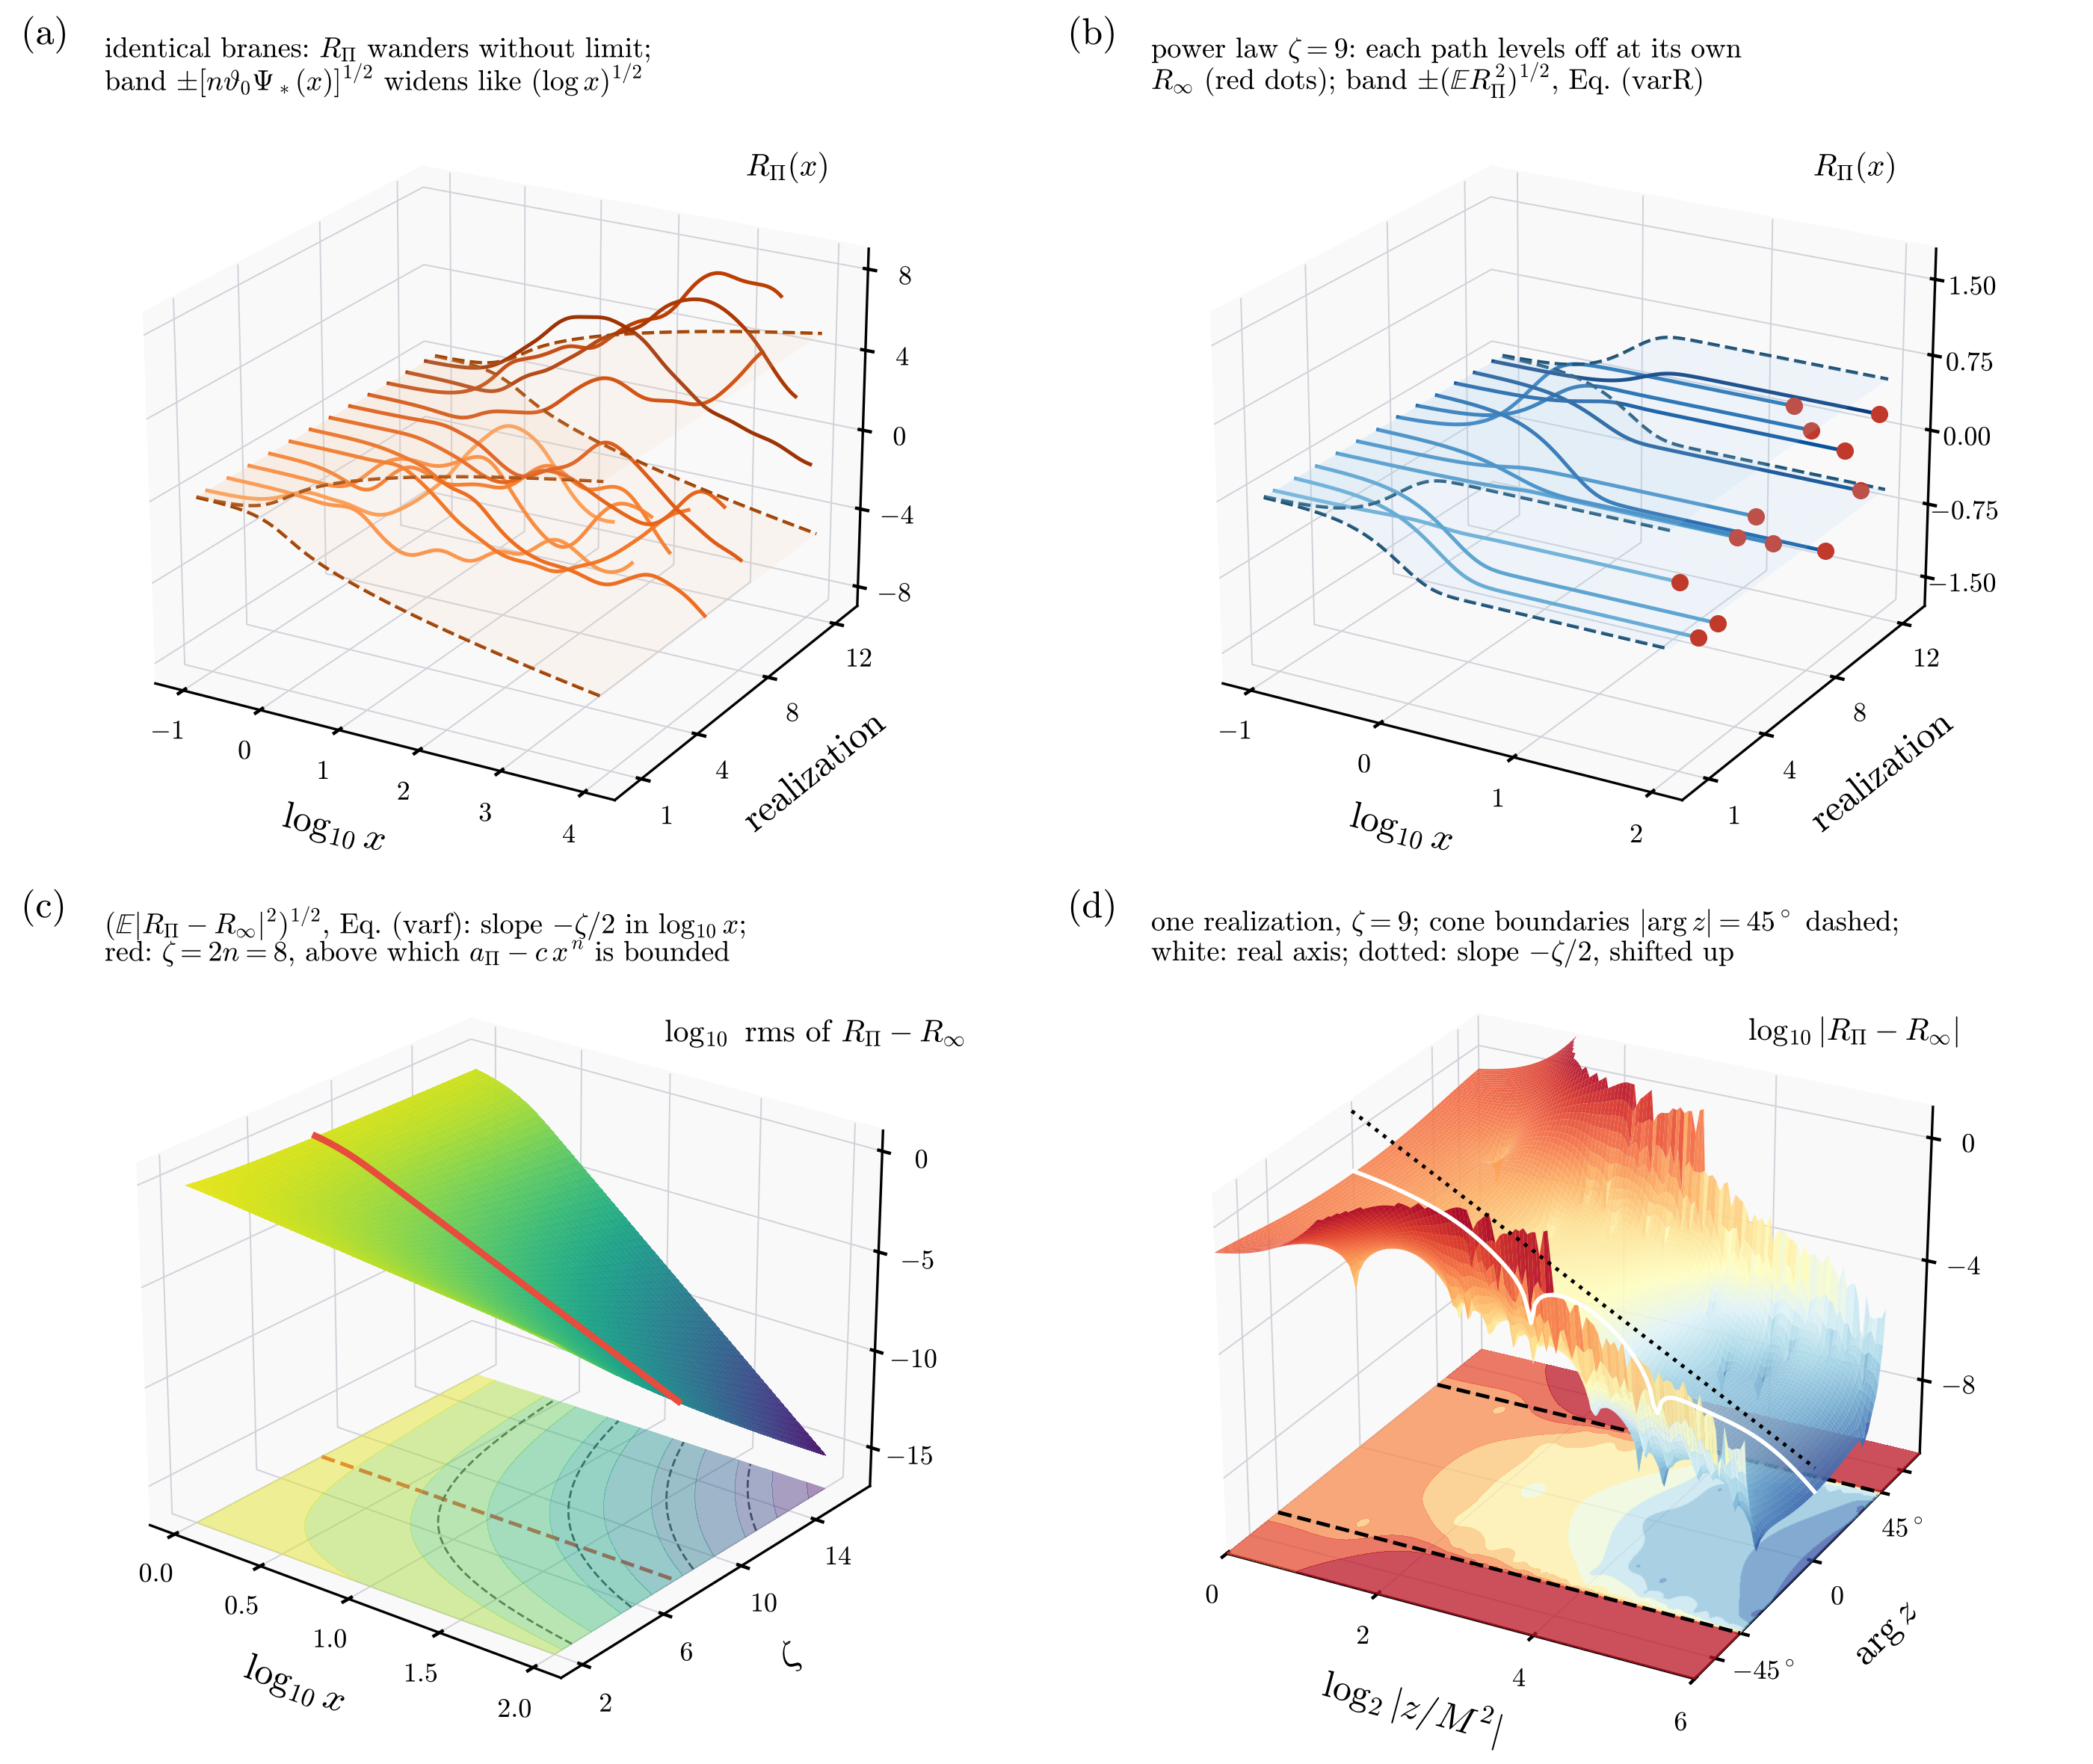
\includegraphics[width=\textwidth]{figs/fig_fluct.png}
\caption{Fluctuations of a realization, for $n=4$, $\vartheta_0=\log2$ and $\psi_*$. (a) Sample paths of $R_\Pi(x)$ for twelve realizations of a gas of identical branes, drawn as ribbons over $\log_{10}x$ and the index of the realization, with the band $\pm(\bE R_\Pi^2)^{1/2}$ of Eq.~\eqref{eq:Psistar} (translucent sheets with dashed edges). The band widens like $(\log x)^{1/2}$ and the paths wander without limit. (b) The same for the fine-grained gas with $\zeta=9$, with the band of Eq.~\eqref{eq:varR}. Each path levels off at its own value of $R_\infty$, marked by a dot at the right end. (c) The root-mean-square remainder $(\bE|R_\Pi-R_\infty|^2)^{1/2}$, Eq.~\eqref{eq:varf}, as a surface over $\log_{10}x$ and $\zeta$, in $\log_{10}$. Its slope in $\log_{10}x$ is $-\zeta/2$; the red line marks $\zeta=2n=8$, above which the remainder of $a_\Pi$ after the monomial is subtracted is bounded; condition (G) asks only for $\zeta>4$. (d) $\log_{10}|R_\Pi(z)-R_\infty|$ for one realization with $\zeta=9$ over the plane of $\log_2|z/M^2|$ and $\arg z$, for $|\arg z|\le72^\circ$, with the cone boundaries $|\arg z|=45^\circ$ (dashed) and the real axis (white). Inside the cone the surface falls along every ray with slope close to $-\zeta/2$ (dotted reference line, shifted up), as Eq.~\eqref{eq:asdecay} states; the dips on the real axis are sign changes of $R_\Pi-R_\infty$. Outside the cone, where (S4) gives no control, the surface rises and is cut off at $10$. In (b) and (d) the branes smaller than $0.3\,M^{-2}$ in the fine-grained gas, about $3\times10^{5}$ per $e$-fold and more, are represented by their Gaussian limit; all other branes are drawn individually.}
\label{fig:fluct}
\end{figure*}

\subsection{What the field theory uses}
\label{sec:uses}

From here on the form factor is that of one realization, and we drop the subscript: $a=a_\Pi$ and $c=c_\Pi$, with the remainder $\mathcal G$ of Eq.~\eqref{eq:G}. Sections~\ref{sec:action}--\ref{sec:unitarity} use $a$ only through the following properties, each proved above for almost every realization of a gas obeying A1 and A2: $a$ is entire, has no zeros, satisfies $a(0)=1$ and has real Taylor coefficients (Sec.~\ref{sec:formfactor}); on the real axis it obeys the two-sided bound~\eqref{eq:twosided-real} and the derivative bounds~\eqref{eq:aderiv}; $\mathcal G$ is a symbol of order $m_\sigma-1$ and $a-cx^n$ a symbol of order $m_\sigma$, with $0\le m_\sigma<n-2$, Eqs.~\eqref{eq:msigma} and \eqref{eq:Gsymbol}; and in the cones of (S4) the asymptotics~\eqref{eq:cone-real} hold, with $|a(z)|\ge\frac c2|z/M^2|^n$ for large $|z|$. Where a statement depends on the realization, the dependence is through $c$, through the bound $C_\Pi$ of Eq.~\eqref{eq:asdecay}, or through $\|R_\Pi\|$; we point it out where it matters. The skeleton enters directly in two places only, the zero-point energy of Sec.~\ref{sec:vacuum}, whose mean it gives, and the Newtonian numbers of Sec.~\ref{sec:classical}. Table~\ref{tab:a} collects the properties of the skeleton and of a realization side by side.

\begin{table*}[t]
\caption{Properties of the skeleton $\hat a=\exp[\frac n2\Ein(x^2)]$ for $\psi_*$, with $\hat c=e^{n\gE/2}$, and of the form factor $a$ of a realization, which hold almost surely for a gas obeying (G). Here $x=z/M^2$, $\varepsilon>0$ is arbitrary and $C$ depends on the realization. All entries are derived in Secs.~\ref{sec:formfactor}--\ref{sec:fluct}; the last column says where each is used.}
\label{tab:a}
\begin{ruledtabular}
\begin{tabular}{L{2.2cm}L{5.9cm}L{5.6cm}L{3.3cm}}
property & skeleton $\hat a$ & realization $a=\hat a\,e^{R_\Pi}$ & used in\\
\colrule
analyticity & entire, no zeros, $\hat a(0)=1$, $\hat a(-z)=\hat a(z)$, real coefficients & entire, no zeros by (S5), $a(0)=1$, $a(-z)=a(z)$, real coefficients & pole content, Sec.~\ref{sec:prop}\\
real axis & $(1+x^2)^{n/2}\le\hat a\le\hat c\,(1+x^2)^{n/2}$ & same, with factors $e^{\mp\|R_\Pi\|}$, Eq.~\eqref{eq:twosided-real} & propagator bound~\eqref{eq:propbound}\\
large $|x|$, real & $\hat a=\hat c\,|x|^n\exp[\frac n2E_1(x^2)]$ & $a=c\,|x|^n[1+O(|x|^{-\sigma/2+\varepsilon})]$, $c=\hat c\,e^{R_\infty}$ & local theory, Sec.~\ref{sec:local}\\
small $x$ & $\hat a=1+\frac n2x^2+\frac{n(n-1)}8x^4+O(x^6)$ & $a=1+b_\Pi x^2+O(x^4)$, $b_\Pi=\sum\vartheta(s)s^2M^4$, $\bE\,b_\Pi=\frac n2$ & Newtonian limit, Sec.~\ref{sec:classical}\\
remainder & $\hat{\mathcal G}$ of order $-1$; $\hat a-\hat cx^n$ exponentially small & $\mathcal G$ of order $m_\sigma-1$; $a-cx^n$ of order $m_\sigma<n-2$, Eq.~\eqref{eq:msigma} & vertex bound, Sec.~\ref{sec:vertex}\\
cones & $\hat a=\hat c\,(z/M^2)^n[1+\epsilon]$, $|\epsilon|\lesssim e^{-\mathrm{Re}\,z^2/M^4}$ & $a=c\,(z/M^2)^ne^{\eta_\Pi}$, $|\eta_\Pi|\le C|z/M^2|^{-\sigma/2+\varepsilon}$ & unitarity, Sec.~\ref{sec:unitarity}\\
imaginary axis & $\hat a(iy)\to0$ faster than any exponential & not controlled, not used & Sec.~\ref{sec:unitarity}\\
constant & $\hat c=3.172$, $4.234$, $5.650$, $7.540$, $10.063$ for $n=4,\dots,8$ & $\log c$ has mean $\log\hat c$, variance $nV(1)$ & one-loop tuning, Sec.~\ref{sec:killers}\\
other responses & same with $\hat c=e^{nC_+}$, Sec.~\ref{sec:class} & same with $c=e^{nC_++R_\infty}$ & Sec.~\ref{sec:class}\\
\end{tabular}
\end{ruledtabular}
\end{table*}

The two premises are the only places where the brane picture enters. Assumption A1 is a statement about a single brane, (S1)--(S5), which Sec.~\ref{sec:cells} derives from the cell model (M1)--(M3); the model itself is not derived from a brane action. Assumption A2 is a statement about the gas: independence, the scale-invariant strength~\eqref{eq:intensity} and the fine graining (G). No average over realizations is taken anywhere, and no limit of many regions or many samples is needed: the field theory below is that of one frozen gas. Table~\ref{tab:assumptions} records where each input is used.

\begin{table}[t]
\caption{Inputs of the paper, what each is used for, and what fails without it. Everything not listed here is derived, for almost every realization of the gas.}
\label{tab:assumptions}
\begin{ruledtabular}
\begin{tabular}{L{1.95cm}L{3.05cm}L{2.9cm}}
input & used for & if dropped\\
\colrule
cells, (M1)--(M3) & derive (S1)--(S5) and $\psi=\psi_*$ & A1 must be assumed\\
A1, (S1) & $a$ entire with $a(0)=1$ & $F(\Box)$ not entire\\
A1, (S2) & $a\ge1$ on both half-axes & no polynomial bound on one half-axis\\
A1, (S3) & skeleton corrections beyond all powers & $G$ and $\Lambda$ run at one loop\\
A1, (S4) & cone asymptotics~\eqref{eq:cone-gen}, \eqref{eq:cone-real} & cutting rules not established\\
A1, (S5) & no zeros in any realization & complex pole pairs, Eq.~\eqref{eq:qzeros}\\
A2, independence & Poisson gas & formulas of Sec.~\ref{sec:avg} lost\\
A2, Eq.~\eqref{eq:intensity} & growth $|x|^n$ with integer $n$ & no fixed power\\
A2, (G) & $a-cx^n=O(x^{m_\sigma})$, Eq.~\eqref{eq:Gsymbol}; finite $\delta\rho_\Pi$ & $\zeta\le4$: $\delta\rho_\Pi$ diverges; identical branes: no limit of $a/x^n$\\
$\psi=\psi_*$ & closed forms; numbers of Sec.~\ref{sec:classical} & other constants, Table~\ref{tab:class}\\
$n$ integer & local theory polynomial & no local split\\
$n\ge4$ & every graph with $L\ge2$ converges & $n=3$: $\bar\omega(2)=0$\\
\end{tabular}
\end{ruledtabular}
\end{table}

\section{Action, propagator and spectrum}
\label{sec:action}

\subsection{The action}

Let $g_{\mu\nu}=\eta_{\mu\nu}+\kappa h_{\mu\nu}$ with $\kappa^2=32\pi G$, and $G_{\mu\nu}=R_{\mu\nu}-\frac12g_{\mu\nu}R$. The Euclidean action is
\begin{multline}
\label{eq:action}
S=-\frac2{\kappa^2}\int\dd^4x\sqrt g\,\bigl[R+G_{\mu\nu}F(\Box)R^{\mu\nu}\bigr]+S_{\rm q},\\
F(\Box)=\frac{a(-\Box)-1}{\Box},
\end{multline}
where $S_{\rm q}$ collects three operators quartic in curvature, introduced in Sec.~\ref{sec:killers}. Being quartic, they contribute nothing to the quadratic or cubic terms of the action around flat space. Since $a(0)=1$, $F$ is an entire function of $\Box$. The combination $G_{\mu\nu}F(\Box)R^{\mu\nu}$ is the one used in Refs.~\cite{Tomboulis1997,Modesto2012}, and the reason for it appears below: around flat space it multiplies the whole Einstein operator by one function.

\subsection{Linearized curvature}

We use the spin projectors of Barnes and Rivers~\cite{Rivers1964,VanNieuwenhuizen1973}. With $\theta_{\mu\nu}=\delta_{\mu\nu}-p_\mu p_\nu/p^2$ and $\omega_{\mu\nu}=p_\mu p_\nu/p^2$, in $D$ dimensions,
\begin{align*}
\Pt_{\mu\nu\alpha\beta}&=\tfrac12(\theta_{\mu\alpha}\theta_{\nu\beta}+\theta_{\mu\beta}\theta_{\nu\alpha})-\tfrac1{D-1}\theta_{\mu\nu}\theta_{\alpha\beta},\\
(\Ps)_{\mu\nu\alpha\beta}&=\tfrac1{D-1}\theta_{\mu\nu}\theta_{\alpha\beta}.
\end{align*}
They are orthogonal idempotents, and both are annihilated by contraction with $p^\mu$. For a metric perturbation $h_{\mu\nu}$ with Fourier transform $h(p)$, the linearized Ricci tensor is
\[
R^{(1)}_{\mu\nu}=\tfrac12\bigl(-p_\rho p_\mu h^\rho{}_\nu-p_\rho p_\nu h^\rho{}_\mu+p^2h_{\mu\nu}+p_\mu p_\nu h\bigr),
\]
with $h=h^\mu{}_\mu$. Substituting a gauge mode $h_{\mu\nu}=p_\mu\xi_\nu+p_\nu\xi_\mu$, the terms cancel in pairs, so $R^{(1)}$ depends only on the transverse part $(\Pt+\Ps)h$; every symmetric tensor is its transverse part plus a gauge mode, because $1-\Pt-\Ps$ projects onto tensors of the form $p_\mu\xi_\nu+p_\nu\xi_\mu$. For transverse $h$ the formula reduces to $\frac12(p^2h_{\mu\nu}+p_\mu p_\nu h)$, and writing $h_{\mu\nu}=(\Pt h)_{\mu\nu}+(\theta\cdot h)\,\theta_{\mu\nu}/(D-1)$, with $\theta\cdot h=\theta^{\mu\nu}h_{\mu\nu}$, we get
\begin{equation}
\label{eq:Ric1}
R^{(1)}_{\mu\nu}=\frac{p^2}2\Bigl[(\Pt h)_{\mu\nu}+(\theta\!\cdot\!h)\,T_{\mu\nu}\Bigr],\qquad T_{\mu\nu}=\frac{\theta_{\mu\nu}}{D-1}+\omega_{\mu\nu}.
\end{equation}
Its trace is $R^{(1)}=p^2\,\theta\cdot h$. Squaring Eq.~\eqref{eq:Ric1}, the cross terms vanish because $\Pt h$ is transverse and traceless, $T\cdot T=D/(D-1)$, and $(\theta\cdot h)^2=(D-1)\,h\Ps h$, where $hPh$ stands for $h^{\mu\nu}P_{\mu\nu\alpha\beta}h^{\alpha\beta}$ and products are understood as $h(-p)\cdots h(p)$. This gives
\begin{align}
R^{(1)}_{\mu\nu}R^{(1)\mu\nu}&=\tfrac{p^4}4\bigl[h\Pt h+D\,h\Ps h\bigr],\label{eq:RicRic}\\
\bigl(R^{(1)}\bigr)^2&=p^4(D-1)\,h\Ps h,\label{eq:RR}\\
G^{(1)}_{\mu\nu}R^{(1)\mu\nu}&=\tfrac{p^4}4\bigl[h\Pt h-(D-2)\,h\Ps h\bigr],\label{eq:GR}\\
h^{\mu\nu}G^{(1)}_{\mu\nu}&=\tfrac{p^2}2\bigl[h\Pt h-(D-2)\,h\Ps h\bigr].\label{eq:hG}
\end{align}
Equation~\eqref{eq:GR} is Eq.~\eqref{eq:RicRic} minus half of Eq.~\eqref{eq:RR}, and Eq.~\eqref{eq:hG} follows from $G^{(1)}=\frac{p^2}2[\Pt h-\frac{D-2}{D-1}(\theta\cdot h)\theta]$.

\subsection{Quadratic action and propagator}
\label{sec:prop}

Since $\delta(\sqrt gR)=-\sqrt g\,G^{\mu\nu}\delta g_{\mu\nu}$ up to a total derivative and $G_{\mu\nu}$ vanishes on flat space, the second-order term of $\int\sqrt gR$ is $-\frac12\int\delta g^{\mu\nu}G^{(1)}_{\mu\nu}[\delta g]$, which for $\delta g=\kappa h$ is $-\frac{\kappa^2}2\int h\,G^{(1)}[h]$. The nonlocal term is already quadratic in curvature, so its second-order part is $\kappa^2\int G^{(1)}F(\Box)R^{(1)}$ with $\Box\to-p^2$. With the prefactor $-2/\kappa^2$ and Eqs.~\eqref{eq:GR} and \eqref{eq:hG} at $D=4$, the quadratic action is $\frac12p^2[1-p^2F(-p^2)]\,h[\Pt-2\Ps]h$, and $1-p^2F(-p^2)=1+(a(p^2)-1)=a(p^2)$. Hence
\begin{equation}
\label{eq:S2}
S^{(2)}=\frac12\int\frac{\dd^4p}{(2\pi)^4}\,p^2a(p^2)\;h(-p)\bigl[\Pt-2\Ps\bigr]h(p),
\end{equation}
the Einstein--Hilbert quadratic action multiplied by $a(p^2)$. On the gauge-invariant subspace it is inverted by
\begin{equation}
\label{eq:prop}
\mathcal D(p)=\frac{\Pt-\frac12\Ps}{p^2\,a(p^2)} ,
\end{equation}
the propagator of general relativity divided by $a$.

As a function of $z=p^2\in\bC$, Eq.~\eqref{eq:prop} is analytic except at $z=0$: $a$ is entire and zero-free, so $1/a$ is entire, and $1/(za)$ has a simple pole at the origin with residue $1/a(0)=1$; the projectors do not depend on $|p|$. The residue is that of general relativity, so the exchange between conserved sources at long distances is Einstein's and carries the same positive norm. In Lorentzian signature the only on-shell condition is $p^2=0$, and because the form factor multiplies the spin-two projector by a scalar, both helicities have the dispersion relation $\omega^2=k^2$ at every wavenumber. There are no massive states, ghosts or tachyons in the tree-level spectrum, and the speed of gravitational waves equals that of light identically.\footnote{The bound from GW170817 and GRB~170817A is $-3\times10^{-15}<(c_g-c)/c<7\times10^{-16}$~\cite{GW170817}. Theories with a momentum-dependent spin-two form factor that is not shared by the whole Einstein operator generically violate it at some wavenumber; here the factorized structure~\eqref{eq:S2} prevents that.}

For comparison, a polynomial form factor of degree $N$ has $N$ extra poles whose residues add up to $-1$, by the residue theorem applied to $1/(za)$~\cite{Shapiro2015}; Stelle's theory is $N=1$, with residue exactly $-1$~\cite{Stelle1977}. A frozen gas of resonant branes would have infinitely many complex pairs, Eq.~\eqref{eq:qzeros}; a realization of the gas of Sec.~\ref{sec:gas}, whose branes have no resonances, has no extra pole at all.

\section{Ultraviolet power counting}
\label{sec:power}

\subsection{Gauge fixing and ghosts}
\label{sec:gf}

We use the background-field method~\cite{Abbott1981}, $g=\bar g+\kappa h$, with the background-covariant de Donder condition $\chi_\mu=\bar\nabla^\nu h_{\mu\nu}-\frac12\bar\nabla_\mu h$ and the weighted gauge-fixing term
\begin{equation}
\label{eq:gf}
S_{\rm gf}=\int\dd^4x\sqrt{\bar g}\;\chi_\mu\,a(-\bar\Box)\,\chi^\mu .
\end{equation}
For $a=1$ this is the Feynman--de Donder term, which added to the Einstein part of Eq.~\eqref{eq:S2} gives the operator $p^2(\mathbf 1-\frac12\delta\otimes\delta)$, with $\mathbf 1$ the identity on symmetric tensors.\footnote{In four dimensions $(\mathbf 1-\frac12\delta\otimes\delta)^2=\mathbf 1-\delta\otimes\delta+\frac14(\delta\cdot\delta)\,\delta\otimes\delta=\mathbf 1$, since $\delta\cdot\delta=4$. The normalization of Eq.~\eqref{eq:gf}, coefficient one in front of $\chi_\mu\chi^\mu$ with the action normalized as in Eq.~\eqref{eq:S2}, is the one that makes the trace and traceless parts combine in this way.} Around flat space both the gauge-invariant part and the gauge-fixing part are those of general relativity multiplied by $a(p^2)$, so the full propagator is
\begin{equation}
\label{eq:propfull}
\mathcal D_{\mu\nu\alpha\beta}(p)=\frac{\frac12(\delta_{\mu\alpha}\delta_{\nu\beta}+\delta_{\mu\beta}\delta_{\nu\alpha})-\frac12\delta_{\mu\nu}\delta_{\alpha\beta}}{p^2\,a(p^2)}.
\end{equation}
The weight $Y=a(-\bar\Box)$ is handled in the standard way~\cite{Nielsen1978,Kallosh1978}. Averaging the gauge condition with the Gaussian weight $e^{-\int fYf}$ requires the normalization $(\det Y)^{1/2}$; combined with the Faddeev--Popov determinant $\det Q$, where $Q$ is the usual second-order ghost operator, this is $\det(YQ)\,(\det Y)^{-1/2}$. The ghosts therefore get the action $\bar c^\mu YQ_{\mu\nu}c^\nu$, and a factor $(\det Y)^{-1/2}$ depending on the background alone compensates; it contributes $+\frac12\Tr\log a(-\bar\Box)$ to the effective action and has no vertices with quantum fields. The ghost propagator is $\delta_{\mu\nu}/(p^2a(p^2))$. Every propagator of the theory, graviton or ghost, is then bounded by
\begin{equation}
\label{eq:propbound}
|\mathcal D(p)|\le\frac{C}{p^2(1+p^2/M^2)^{n}},
\end{equation}
by the lower bound in Eq.~\eqref{eq:twosided-real} and $1+x^2\ge\frac12(1+x)^2$; the constant $C$ depends on the realization through $\|R_\Pi\|$.

\subsection{Functions of the d'Alembertian in perturbation theory}
\label{sec:DK}

The vertices of a nonlocal theory come from expanding $F(\Box)$, $a(-\bar\Box)$ and the like in powers of the fields, and a standard formula for functions of perturbed operators organizes this~\cite{DaletskiiKrein1965}. For points $z_0,\dots,z_m$ the divided difference $f[z_0,\dots,z_m]$ is defined by $f[z_0]=f(z_0)$ and
\[
f[z_0,\dots,z_m]=\frac{f[z_1,\dots,z_m]-f[z_0,\dots,z_{m-1}]}{z_m-z_0},
\]
extended to coincident points by continuity. It is symmetric in its arguments and obeys the Hermite--Genocchi formula~\cite{deBoor2005}
\begin{equation}
\label{eq:HG}
f[z_0,\dots,z_m]=\int_{\Sigma_m}f^{(m)}\Bigl(\sum_{i=0}^m t_iz_i\Bigr)\dd t,
\end{equation}
where $\Sigma_m=\{t_i\ge0,\sum t_i=1\}$ carries Lebesgue measure of total mass $1/m!$.

Let $A+B$ act on plane waves, with $A$ diagonal, $Ae^{iq\cdot x}=z(q)e^{iq\cdot x}$. For entire $f$, the term of $f(A+B)$ of order $m$ in $B$, acting on $e^{iq_0\cdot x}$ and projected on $e^{iq_m\cdot x}$, is
\begin{equation}
\label{eq:DK}
\sum_{q_1,\dots,q_{m-1}}f[z_0,\dots,z_m]\;B_{q_mq_{m-1}}\cdots B_{q_1q_0},\qquad z_i=z(q_i),
\end{equation}
summed over the intermediate momenta that $B$ allows. Appendix~\ref{app:dd} gives the short proof. In perturbation theory $A=-\Box_0$ with $z(q)=q^2$, and $B=-(\Box-\Box_0)$ collects the terms of the covariant d'Alembertian with at least one power of the fields. Each insertion of $B$ is a polynomial in the fields with at most two derivatives, which act either on the fields of the insertion or on the operand. Figure~\ref{fig:chain} shows the structure.

\begin{figure*}[t]
\centering
\begin{minipage}[c]{0.53\textwidth}\centering
\resizebox{\linewidth}{!}{%
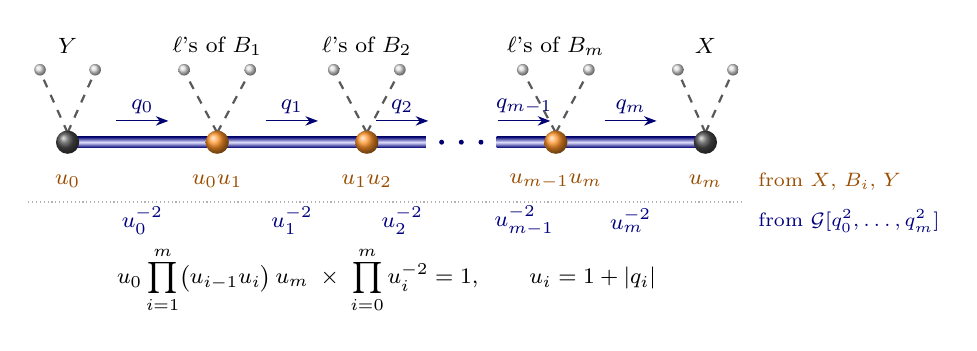
\begin{tikzpicture}[font=\footnotesize,>={Stealth[length=1.6mm]}]
\def\tube#1#2{\shade[top color=blue!45!black,bottom color=blue!45!black,middle color=blue!12] (#1,-0.07) rectangle (#2,0.07);}
\tube{0}{4.55}\tube{5.45}{8.1}
\foreach \xx in {4.75,5.0,5.25} \fill[blue!45!black] (\xx,0) circle (0.9pt);
\foreach \xx/\yy in {1.9/0,3.8/0,6.2/0} {
  \draw[bkg] (\xx,0.12) -- ++(-0.42,0.78); \draw[bkg] (\xx,0.12) -- ++(0.42,0.78);
  \shade[ball color=gray!25] (\xx-0.42,0.92) circle (2.1pt); \shade[ball color=gray!25] (\xx+0.42,0.92) circle (2.1pt);
}
\draw[bkg] (0,0.12) -- ++(-0.35,0.78); \draw[bkg] (0,0.12) -- ++(0.35,0.78);
\shade[ball color=gray!25] (-0.35,0.92) circle (2.1pt); \shade[ball color=gray!25] (0.35,0.92) circle (2.1pt);
\draw[bkg] (8.1,0.12) -- ++(-0.35,0.78); \draw[bkg] (8.1,0.12) -- ++(0.35,0.78);
\shade[ball color=gray!25] (7.75,0.92) circle (2.1pt); \shade[ball color=gray!25] (8.45,0.92) circle (2.1pt);
\node at (1.9,1.22) {$\ell$'s of $B_1$}; \node at (3.8,1.22) {$\ell$'s of $B_2$}; \node at (6.2,1.22) {$\ell$'s of $B_m$};
\node at (0,1.22) {$Y$}; \node at (8.1,1.22) {$X$};
\shade[ball color=black!70] (0,0) circle (4.2pt); \shade[ball color=black!70] (8.1,0) circle (4.2pt);
\foreach \xx/\lab in {1.9/1,3.8/2,6.2/m} \shade[ball color=orange!85] (\xx,0) circle (4.2pt);
\foreach \xx/\lab in {0.95/0,2.85/1,4.25/2,5.8/{m-1},7.15/m} \draw[->,blue!45!black] (\xx-0.33,0.27) -- node[above=-1pt] {$q_{\lab}$} (\xx+0.33,0.27);
\node[orange!60!black] at (0,-0.5) {$u_0$};
\node[orange!60!black] at (1.9,-0.5) {$u_0u_1$};
\node[orange!60!black] at (3.8,-0.5) {$u_1u_2$};
\node[orange!60!black] at (6.2,-0.5) {$u_{m-1}u_m$};
\node[orange!60!black] at (8.1,-0.5) {$u_m$};
\foreach \xx/\lab in {0.95/0,2.85/1,4.25/2,5.8/{m-1},7.15/m} \node[blue!50!black] at (\xx,-1.0) {$u_{\lab}^{-2}$};
\draw[gray!60,densely dotted] (-0.5,-0.76) -- (8.6,-0.76);
\node[align=center] at (4.05,-1.75) {$\displaystyle u_0\prod_{i=1}^m\bigl(u_{i-1}u_i\bigr)\,u_m\;\times\;\prod_{i=0}^mu_i^{-2}=1,\qquad u_i=1+|q_i|$};
\node[anchor=west,orange!60!black,font=\scriptsize] at (8.65,-0.5) {from $X$, $B_i$, $Y$};
\node[anchor=west,blue!50!black,font=\scriptsize] at (8.65,-1.0) {from $\mathcal G[q_0^2,\dots,q_m^2]$};
\end{tikzpicture}}
\end{minipage}\hfill
\begin{minipage}[c]{0.44\textwidth}\centering
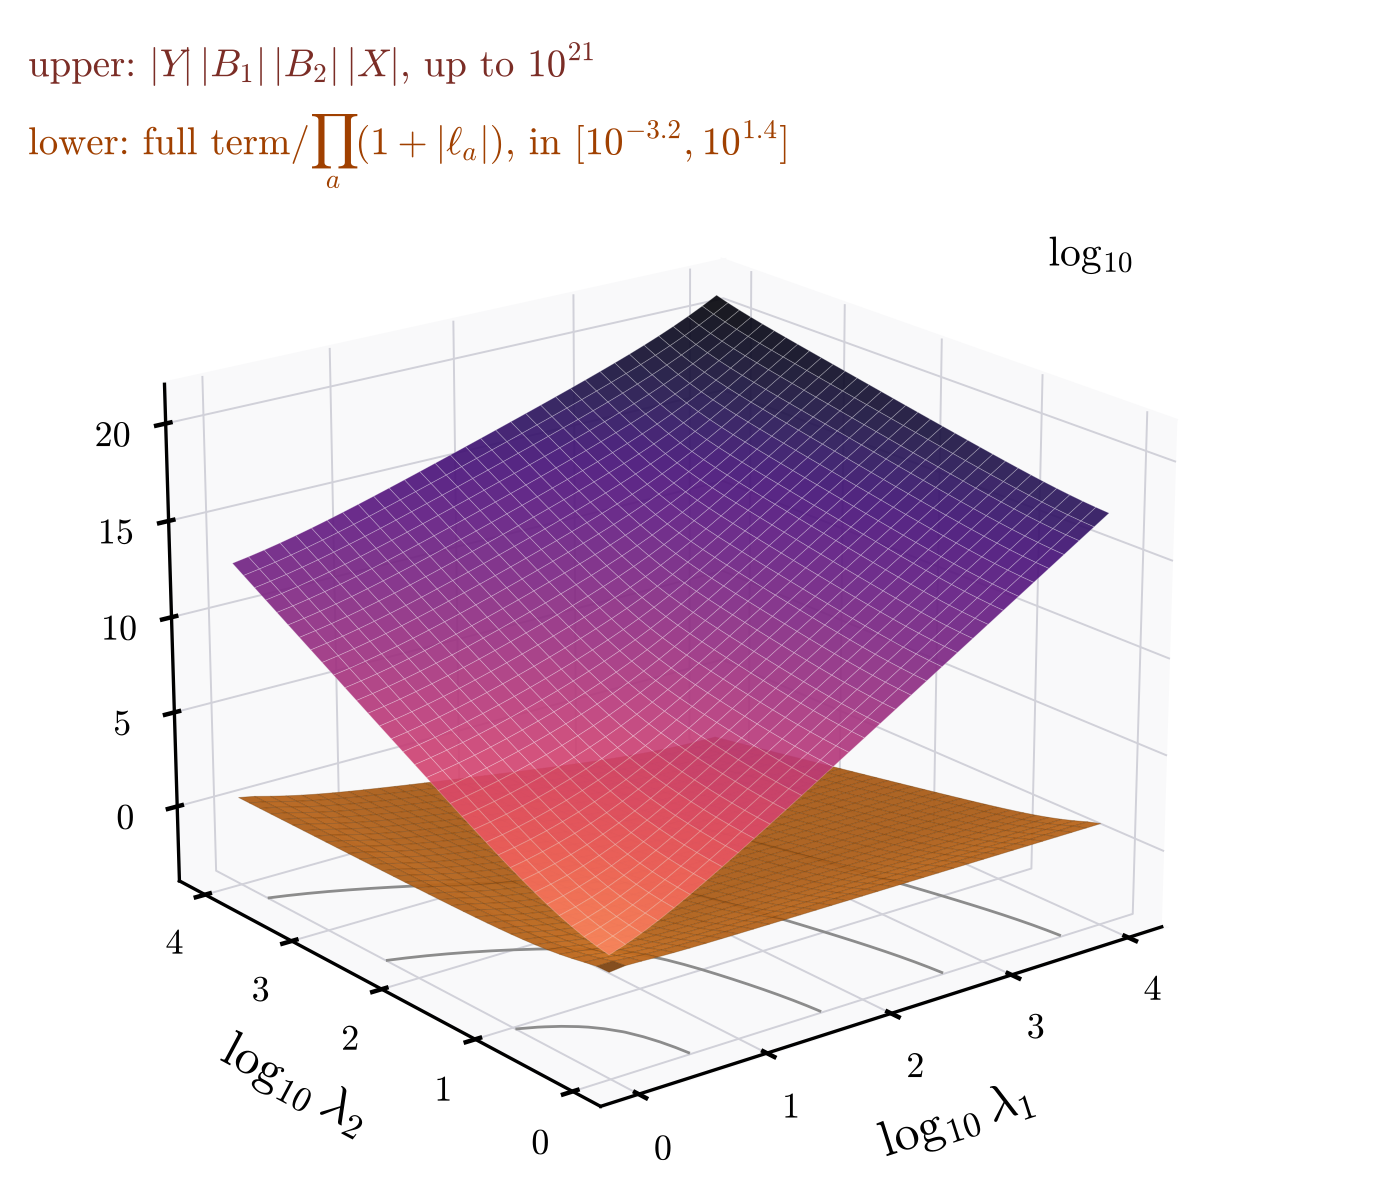
\includegraphics[width=\linewidth]{figs/fig_chain3d.png}
\end{minipage}
\caption{The chain behind the vertex bound. (a) A function of the covariant d'Alembertian between two field monomials, $X\,\mathcal G(-\Box)\,Y$, expanded as in Eq.~\eqref{eq:DK}. Each insertion $B_i$ of the field-dependent part of $\Box$ attaches legs (dashed, gray balls) and changes the running momentum from $q_{i-1}$ to $q_i$; the function enters only through the divided difference $\mathcal G[q_0^2,\dots,q_m^2]$. By Eq.~\eqref{eq:insertion} each insertion costs one power of the running momentum on each side of it (orange), and $Y$ and $X$ one power each; by Eq.~\eqref{eq:ddbound} the divided difference returns $u_i^{-2}$ for every segment (blue). The running momenta cancel exactly, and only the legs are left. (b) A numerical check of this bookkeeping for a chain with two insertions and $n=4$, in units $M=1$. The running momenta are $q_0=\ell_Y$ with $|q_0|=1$, $q_1=q_0+\ell_1$ with $|q_1|\simeq\lambda_1$, and $q_2=q_1+\ell_2$ with $|q_2|\simeq\lambda_2$; each insertion is given its largest size $(|q_{i-1}|+|\ell_i|)^2$ and $X$, $Y$ the sizes $u_2$, $u_0$. The upper surface is $\log_{10}$ of the product of these sizes, which grows like the fifth power of the momenta, to $10^{21}$; the lower surface is $\log_{10}$ of the full term, with the exact divided difference of the skeleton's $\hat{\mathcal G}$, divided by $(1+|\ell_1|)(1+|\ell_2|)$. It stays between $10^{-3.2}$ and $10^{1.4}$ over the four decades in $\lambda_1$ and $\lambda_2$.}
\label{fig:chain}
\end{figure*}

The divided differences that appear are those of $\mathcal G$, of $a-cx^n$ and of polynomials. For the first two we need a bound that controls mixed configurations, in which some of the $z_i$ are large and others small. Let $f$ be smooth on $[0,\infty)$ with $|f^{(j)}(z)|\le C_j(1+z)^{\mu-j}$ for all $j$, for some real $\mu$, and write $\mu_-=\min(\mu,0)$ and $\mu_+=\max(\mu,0)$. Then for every $m$ there is a constant $K_m$ such that, for all $z_0,\dots,z_m\ge0$,
\begin{multline}
\label{eq:ddbound}
\bigl|f[z_0,\dots,z_m]\bigr|\\
\le K_m\,(1+z_{\min})^{\mu_-}(1+z_{\max})^{\mu_+}\prod_{i\ne i_{\min}}(1+z_i)^{-1},
\end{multline}
where $z_{\min}=z_{i_{\min}}$ is a smallest argument and $z_{\max}$ a largest one. The proof, by induction on $m$ using Eq.~\eqref{eq:HG} when the arguments are comparable and the recursion when they are not, is in Appendix~\ref{app:dd}. The bound says that a divided difference of a symbol of order $\mu\le0$ decays like the symbol in its smallest argument and like an inverse power in each of the others; for $\mu>0$ the growth of the symbol is charged to the largest argument.

\subsection{Vertex bound}
\label{sec:vertex}

Consider any vertex of the gauge-fixed action, ghost vertices and the quartic operators $S_{\rm q}$ included, with quantum legs carrying Euclidean momenta $\ell_1,\dots,\ell_N$ and background legs carrying momenta in a fixed bounded set. We show that, for every $n\ge1$,
\begin{multline}
\label{eq:vertexbound}
|V|\le C\,\Bigl[\Bigl(1+\frac{|\ell|_{\max}}{M}\Bigr)^{2n+2}\\
+\Bigl(1+\frac{|\ell|_{\max}}{M}\Bigr)^{2m_\sigma}\prod_{j=1}^N\Bigl(1+\frac{|\ell_j|}{M}\Bigr)\Bigr],
\end{multline}
with $|\ell|_{\max}$ the largest $|\ell_j|$, $m_\sigma$ the order of Eq.~\eqref{eq:msigma}, and $C$ independent of the momenta. The first term bounds the local part of the vertex and the second bounds everything else. When all momenta at a vertex are of order $\lambda$ the first term grows like $\lambda^{2n+2}$, as dimensional analysis requires. The second term grows by one power of $\lambda$ for each hard leg, however many there are, times the fixed power $\lambda^{2m_\sigma}$, which is absent when $\sigma>2n$.

Set $M=1$. Background fields never run in loops, so their momenta are external and bounded in every graph, by $P$ say. By Eq.~\eqref{eq:G}, $F(\Box)=-c(-\Box)^{n-1}-\mathcal G(-\Box)$, and we also split $a(-\bar\Box)=c(-\bar\Box)^n+[a-cx^n](-\bar\Box)$. Every vertex is then a sum of terms of three kinds.

The first kind are local. They come from $c\,G_{\mu\nu}(-\Box)^{n-1}R^{\mu\nu}$, from $S_{\rm q}$, and from the local parts $c(-\bar\Box)^n$ of the gauge-fixing and ghost actions. Each is a polynomial in the momenta of total degree at most $2n+2$, whatever the number of legs, so it is bounded by $C(\sum_j|\ell_j|+P)^{2n+2}\le C(1+|\ell|_{\max})^{2n+2}$.

The second kind contain no function of the full d'Alembertian. They come from the Einstein--Hilbert term, which has two derivatives, and from the remainders $[a-cx^n](-\bar\Box)$ in the gauge-fixing and ghost actions. In those two actions the weight stands between two factors $\chi_\mu$ that are linear in the quantum field, or acts on $Q_{\mu\nu}c^\nu$, where $Q$ has two derivatives, so the quantum legs enter through at most two derivatives. The d'Alembertian inside the weight is the background one. Expanding it by Eq.~\eqref{eq:DK} produces only background insertions, each of which multiplies the operand by at most $C(1+|q|)^2$, with $q$ the running momentum. Since background momenta are bounded, all running momenta of such a chain lie within a fixed distance of one another, and by Eq.~\eqref{eq:ddbound} the divided difference of the symbol $a-cx^n$, of order $m_\sigma$, is at most $C(1+q^2)^{m_\sigma}$ times a factor $(1+q^2)^{-1}$ for every insertion. Every term of the second kind is therefore bounded by $C(1+|\ell|_{\max})^{2+2m_\sigma}$. Momentum conservation gives $|\ell|_{\max}\le(N-1)|\ell_{(2)}|+P$, with $\ell_{(2)}$ the second largest quantum momentum, so $(1+|\ell|_{\max})^2\le C(1+|\ell_{(1)}|)(1+|\ell_{(2)}|)$, and the term lies within the second term of Eq.~\eqref{eq:vertexbound}. (For $N=1$ the single quantum momentum is bounded by $P$, and there is nothing to prove.)

The third kind contain $\mathcal G(-\Box)$ with the full d'Alembertian, in the form $X\,\mathcal G(-\Box)\,Y$, where $X$ comes from $\sqrt g\,G_{\mu\nu}$ and $Y$ from $R^{\mu\nu}$. Here the insertions carry quantum legs, which may be hard, and the estimate has to be made with some care. By Eq.~\eqref{eq:DK} the term of order $m$ is $\mathcal G[z_0,\dots,z_m]\,B_m\cdots B_1$, with $z_i=q_i^2$. The running momentum $q_0$ is the total momentum of the legs of $Y$, and $q_i=q_{i-1}+\sum_{a\in i}\ell_a$, the sum running over the legs of the $i$th insertion. Write $u_i=1+|q_i|$ and $s_i=\sum_{a\in i}|\ell_a|$. An insertion has at most two derivatives, acting on its own legs or on the operand, so $|B_i|\le C(|q_{i-1}|+s_i)^2$; in the same way $|Y|\le Cs_Y^2$ and $|X|\le Cs_X^2$. The estimate that does the work, proved in Appendix~\ref{app:dd}, is
\begin{equation}
\label{eq:insertion}
\bigl(|q|+s\bigr)^2\le C_r\,(1+|q|)(1+|q'|)\prod_{a=1}^r\bigl(1+|\ell_a|\bigr),
\end{equation}
for any $q$ and legs $\ell_1,\dots,\ell_r$, with $q'=q+\sum_a\ell_a$ and $s=\sum_a|\ell_a|$. An insertion costs one power of each of the two running momenta next to it and one power of each of its own legs. Applying Eq.~\eqref{eq:insertion} to every insertion, to $Y$ (with $q=0$, $q'=q_0$) and to $X$ (with $q=0$, $q'=-q_m$, since the legs of $X$ carry away the momentum $q_m$), the running momenta enter through
\[
u_0\,u_m\prod_{i=1}^mu_{i-1}u_i=\prod_{i=0}^mu_i^2 .
\]
On the other side, $\mathcal G$ is a symbol of order $m_\sigma-1$ by Eq.~\eqref{eq:Gsymbol}, and Eq.~\eqref{eq:ddbound} with $\mu=m_\sigma-1$ gives
\begin{align*}
|\mathcal G[z_0,\dots,z_m]|&\le K(1+z_{\max})^{m_\sigma}\prod_{i=0}^m(1+z_i)^{-1}\\
&\le2^{m+1}K(1+z_{\max})^{m_\sigma}\prod_{i=0}^mu_i^{-2}
\end{align*}
whether $\mu$ is negative or positive.\footnote{For $\mu\le0$, Eq.~\eqref{eq:ddbound} gives $(1+z_{\min})^{m_\sigma-1}\prod_{i\ne i_{\min}}(1+z_i)^{-1}$, and $(1+z_{\min})^{m_\sigma}\le(1+z_{\max})^{m_\sigma}$. For $\mu>0$ it gives $(1+z_{\max})^{m_\sigma-1}\prod_{i\ne i_{\min}}(1+z_i)^{-1}$, and $1+z_{\min}\le1+z_{\max}$. For the skeleton, and whenever $\sigma>2n$, $m_\sigma=0$ and the bound is $K\prod_i(1+z_i)^{-1}$.} The running momenta cancel exactly. Every running momentum is a sum of leg momenta and bounded background momenta, so $1+z_{\max}\le C(1+|\ell|_{\max})^2$, and the term is bounded by $C(1+|\ell|_{\max})^{2m_\sigma}\prod_a(1+|\ell_a|)$ over all its legs. The sum over intermediate momenta in Eq.~\eqref{eq:DK} is a finite sum over the ways of distributing the legs among the insertions, which proves Eq.~\eqref{eq:vertexbound}.\footnote{The cancellation is not an artifact of the bounds. When the running momentum rises from soft to hard at one insertion and falls back at the next, the divided difference is of order $\lambda^{-2}$ and the two insertions of order $\lambda^2$ each, so the term grows like $\lambda^2$ while two hard legs are attached: one power per hard leg, as Eq.~\eqref{eq:vertexbound} says. Appendix~\ref{app:checks} lists a numerical check of the bound on random chains with up to three insertions.}

\subsection{Superficial degree}
\label{sec:degree}

Let $\gamma$ be a connected subgraph with $L$ loops of some graph of the theory, and consider the region in which the loop momenta of $\gamma$ are of order $\lambda\to\infty$ while all other momenta are fixed. Let $\gamma$ have $I$ internal lines and $V$ vertices, so that $I-V=L-1$, and let $h_v$ be the number of lines of $\gamma$ at the vertex $v$, so that $\sum_vh_v=2I$. Every vertex of $\gamma$ has $h_v\ge2$, because a line of $\gamma$ carries loop momentum and momentum conservation at its ends needs a second line that does. Each line contributes at most $C\lambda^{-2n-2}$ by Eq.~\eqref{eq:propbound}. At a vertex of $\gamma$ the legs outside $\gamma$ carry fixed momenta, so Eq.~\eqref{eq:vertexbound} contributes at most $C\lambda^{\max(2n+2,\,h_v+2m_\sigma)}$. The measure contributes $\lambda^{4L}$. With $x_+=\max(x,0)$ and $k_\sigma=2n+2-2m_\sigma$, which exceeds $6$, the superficial degree is therefore at most
\[
\begin{aligned}
&4L-(2n+2)I+\sum_v\max(2n+2,h_v+2m_\sigma)\\
&\qquad=4L-(2n+2)(L-1)+\sum_v\bigl(h_v-k_\sigma\bigr)_+ .
\end{aligned}
\]
The last sum is largest when all the lines beyond the minimum meet at one vertex. Indeed $(a-k)_++(b-k)_+\le(a+b-2-k)_+$ whenever $a,b\ge2$ and $k\ge2$,\footnote{If $a$ and $b$ both exceed $k$, the left side is $a+b-2k\le a+b-2-k$ because $k\ge2$. If only $a$ does, it is $a-k\le a+b-2-k$ because $b\ge2$. If neither does, it is zero.} so merging the vertices one pair at a time gives $\sum_v(h_v-k_\sigma)_+\le(\sum_vh_v-2(V-1)-k_\sigma)_+=(2L-k_\sigma)_+$. Hence the superficial degree of an $L$-loop subgraph is at most
\begin{equation}
\label{eq:omega}
\bar\omega(L)=4L-(2n+2)(L-1)+2\,(L-n-1+m_\sigma)_+ .
\end{equation}
For $m_\sigma=0$ and $L\le n+1$ this is the standard degree $2n+2+(2-2n)L$ of local higher-derivative gravity~\cite{AsoreyLopezShapiro1997,Modesto2012}, and for $L>n+1$ it is $(4-2n)L$. At one loop $\bar\omega(1)=4$ for every $n$. At two loops $\bar\omega(2)=6-2n$, because $m_\sigma<n-2$ keeps the last term at zero. For $L\ge3$ the bound grows with $m_\sigma$, and as $m_\sigma\to n-2$, the weakest fine graining that (G) allows, it tends to $4L-(2n+2)(L-1)+2(L-3)=-(2n-4)(L-1)$. So $\bar\omega(L)<0$ for every $L\ge2$ and every $\sigma>4$ exactly when $n\ge4$. Table~\ref{tab:power} and Fig.~\ref{fig:power} give the numbers.

To turn the degree into a convergence statement we use Weinberg's theorem~\cite{Weinberg1960}. It applies to integrands in his class $A_n$ of functions with power-law behavior along every subspace of the integration variables, with real exponents, a class that contains rational functions and products of real powers of factors $1+|\ell|$ with $\ell$ linear in those variables. It states that the integral converges absolutely if the asymptotic degree of every subspace is negative. On a large-momentum line the factor $1/p^2$ in Eq.~\eqref{eq:propbound} may be replaced by $1/(p^2+\mu^2)$ with any fixed $\mu>0$, which changes nothing in the ultraviolet.\footnote{This separates the ultraviolet from the infrared. Infrared behavior is governed by $a\to1$ and is that of general relativity; it is discussed in Sec.~\ref{sec:finite}.} At each vertex, $(1+|\ell|_{\max})^{p}\le\sum_j(1+|\ell_j|)^{p}$ for $p=2n+2$ and for $p=2m_\sigma$, so the bound~\eqref{eq:vertexbound} is dominated by a finite sum of terms, each either a product $(1+|\ell_k|)^{2m_\sigma}\prod_j(1+|\ell_j|)$ with one ``chosen'' leg $k$ or a single power $(1+|\ell_j|)^{2n+2}$ of one chosen leg. Expanding the product over vertices, the integrand is dominated by a finite sum of functions in $A_n$. In each of them, the degree in the region where $\gamma$ is hard is at most the count above, since a vertex whose chosen leg lies outside $\gamma$ contributes less. Weinberg's theorem therefore applies to each dominating term, and for $n\ge4$ every graph and every subgraph with two or more loops converges in the ultraviolet. The only subgraphs that can diverge are one-loop subgraphs, for which $\bar\omega=4$.

The threshold $n\ge4$ is the one found in the literature by bounding every vertex by $\lambda^{2n+2}$, which is legitimate when all momenta at a vertex are comparable~\cite{AsoreyLopezShapiro1997,Modesto2012}. The vertex bound shows that vertices with many hard legs do not spoil it: the nonlocal remainder gains at most one power of $\lambda$ per hard leg, and a fixed power below $2n-4$ in all, while each hard leg brings a propagator that falls like $\lambda^{-2n-2}$. For $n\le3$ the two-loop degree is not negative and the argument gives nothing. From now on $n\ge4$.

\begin{table}[t]
\caption{Superficial degree $\bar\omega(L)=4L-(2n+2)(L-1)+2(L-n-1+m_\sigma)_+$ from the vertex bound~\eqref{eq:vertexbound}, for $L=1,\dots,5$. Upper block: $m_\sigma=0$, which holds for the skeleton and whenever $\sigma>2n$; for $L\le n+1$ the entries coincide with the standard estimate $2n+2+(2-2n)L$, and the first entry that differs is $n=3$, $L=5$. Lower block: the limit $m_\sigma\to n-2$, the weakest fine graining allowed by (G), which bounds the degree for every $\sigma>4$. Negative entries are convergent.}
\label{tab:power}
\begin{ruledtabular}
\begin{tabular}{cccccc}
$n$ & $L=1$ & $L=2$ & $L=3$ & $L=4$ & $L=5$\\
\colrule
3 & 4 & 0 & $-4$ & $-8$ & $-10$\\
4 & 4 & $-2$ & $-8$ & $-14$ & $-20$\\
5 & 4 & $-4$ & $-12$ & $-20$ & $-28$\\
6 & 4 & $-6$ & $-16$ & $-26$ & $-36$\\
7 & 4 & $-8$ & $-20$ & $-32$ & $-44$\\
8 & 4 & $-10$ & $-24$ & $-38$ & $-52$\\
\colrule
\multicolumn{6}{l}{$m_\sigma\to n-2$ ($\sigma\to4$)}\\
3 & 4 & 0 & $-4$ & $-6$ & $-8$\\
4 & 4 & $-2$ & $-8$ & $-12$ & $-16$\\
5 & 4 & $-4$ & $-12$ & $-18$ & $-24$\\
6 & 4 & $-6$ & $-16$ & $-24$ & $-32$\\
7 & 4 & $-8$ & $-20$ & $-30$ & $-40$\\
8 & 4 & $-10$ & $-24$ & $-36$ & $-48$\\
\end{tabular}
\end{ruledtabular}
\end{table}

\begin{figure}[t]
\centering
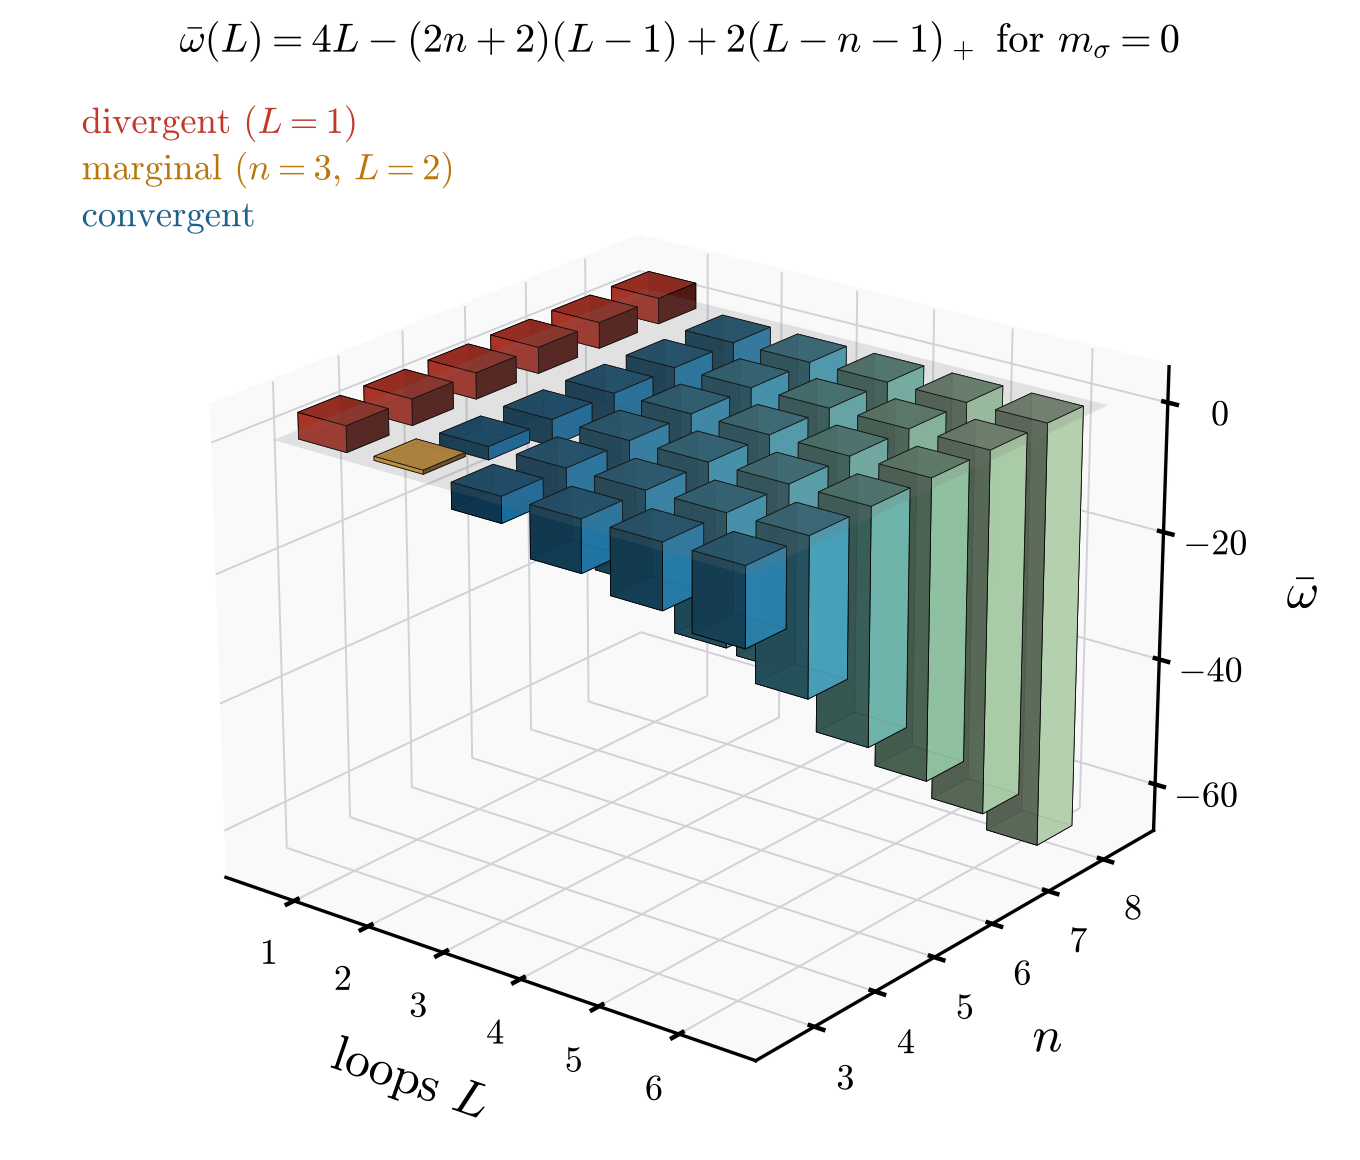
\includegraphics[width=\columnwidth]{figs/fig_power.png}
\caption{Upper bound $\bar\omega(L)$ on the superficial degree of an $L$-loop graph, Eq.~\eqref{eq:omega}, for $n=3,\dots,8$ and $L\le6$, drawn as bars hanging from the plane $\bar\omega=0$. One-loop graphs have degree $4$ for every $n$ (red). For $n=3$ the two-loop bound is $0$ (amber), so power counting alone leaves a possible logarithm; for $n\ge4$ every graph with $L\ge2$ has negative degree (blue to green), and the degree falls without bound as $L$ grows. The bars are drawn for $m_\sigma=0$, which holds for the skeleton and whenever $\sigma>2n$; the lower block of Table~\ref{tab:power} gives the bound for the weakest fine graining, $m_\sigma\to n-2$, which is negative for $L\ge2$ as well.}
\label{fig:power}
\end{figure}

\section{One loop}
\label{sec:oneloop}

\subsection{The local theory}
\label{sec:local}

Split the action into a local part and a remainder,
\begin{align}
S_{\rm loc}&=\frac{2c}{\kappa^2M^{2n}}\int\sqrt g\,G_{\mu\nu}(-\Box)^{n-1}R^{\mu\nu}+S_{\rm q},\label{eq:Sloc}\\
S_{\rm rest}&=-\frac2{\kappa^2}\int\sqrt g\,\bigl[R-G_{\mu\nu}\,\mathcal G(-\Box)\,R^{\mu\nu}\bigr],\notag
\end{align}
so that $S=S_{\rm loc}+S_{\rm rest}$ by Eq.~\eqref{eq:G}. Split the gauge-fixing weight in the same way, $a(-\bar\Box)=c(-\bar\Box/M^2)^n+[a-cx^n](-\bar\Box)$. Both parts of the action are separately invariant under diffeomorphisms, and both parts of the gauge-fixing term are background covariant. The local theory, with action $S_{\rm loc}$, gauge-fixing weight $c(-\bar\Box/M^2)^n$ and the corresponding ghosts, is therefore a consistent background-gauge-fixed theory on its own. Its flat-space propagator is $M^{2n}(\Pt-\frac12\Ps)/(c\,p^{2n+2})$ on the gauge-invariant subspace, from Eq.~\eqref{eq:prop} with $a$ replaced by $cx^n$.

The local theory is badly behaved in the infrared, since its propagator falls like $p^{-2n-2}$ at small $p$ as well as at large $p$. This does not matter for what follows, because we compare the two theories only at large loop momentum. We define the ultraviolet pole of a one-loop integral as the pole, in dimensional regularization with $D=4-2\epsilon$, of its integral over the region $|k|\ge M$ of the loop momentum.\footnote{For a one-loop integrand $I(k,p)$ with bounded external momenta $p$, the region $|k|\ge M$ can be split into $M\le|k|\le K$, which is compact and gives no pole, and $|k|\ge K$ with $K$ large compared with the external momenta, where $I$ may be expanded in $p$. Only the terms of the expansion that are homogeneous of degree $-D$ in $k$ produce a pole, and their coefficients are polynomials in $p$. The pole is therefore local and independent of the choice of $M$ and $K$. With this definition $\int_{|k|\ge M}\dd^Dk\,(2\pi)^{-D}k^{-4}=1/(16\pi^2\epsilon)+O(1)$.} With this definition the ultraviolet pole of the full theory and that of the local theory can be compared graph by graph.

\subsection{One-loop poles are those of the local theory}
\label{sec:poles1}

Let $n\ge4$, and consider any one-loop graph of the full theory with external legs, background or quantum, of bounded momenta. Write each vertex as $V=V_{\rm loc}+V_{\rm rest}$ and each propagator as $\mathcal D=\mathcal D_{\rm loc}+\mathcal D_{\rm rest}$, where the local pieces are those of the local theory. For loop momentum $|k|\ge M$ we have $|V_{\rm loc}|\le C|k|^{2n+2}$ and $|\mathcal D_{\rm loc}|\le C|k|^{-2n-2}$. The remainders are smaller. A remainder vertex consists of terms of the second and third kinds of Sec.~\ref{sec:vertex}, which are bounded by the second term of Eq.~\eqref{eq:vertexbound}; two of its legs carry the loop momentum, so $|V_{\rm rest}|\le C|k|^{2+2m_\sigma}$. And $|\mathcal D_{\rm rest}|\le C|k|^{-2n-2-\sigma+2\varepsilon}$, because $1/a-1/(cx^n)=(cx^n)^{-1}(e^{-\eta_\Pi}-1)$ with $\eta_\Pi$ bounded by Eq.~\eqref{eq:cone-real}. Expanding the product around the loop, the term with only local factors is the integrand of the local theory. Every other term contains at least one $V_{\rm rest}$ or one $\mathcal D_{\rm rest}$. For a loop with $r$ vertices it is bounded for $|k|\ge M$ either by $C|k|^{(2n+2)(r-1)+2+2m_\sigma-(2n+2)r}=C|k|^{2m_\sigma-2n}$, if it contains a remainder vertex, or by $C|k|^{-\sigma+2\varepsilon}$, if it contains a remainder propagator. Both exponents are below $-4$, because $m_\sigma<n-2$ and $\sigma-2\varepsilon>4$. Its integral over $|k|\ge M$ therefore converges in a range of $D$ that contains $D=4$, and has no pole there. The ultraviolet pole of the full graph is that of the local graph.

The compensating factor of Sec.~\ref{sec:gf} contributes $\frac12\Tr\log a(-\bar\Box)$, which at large Euclidean momenta equals $\frac n2\Tr\log(-\bar\Box/M^2)+\frac12\log c\,\Tr\mathbf 1+\frac12\Tr\,\eta_\Pi(-\bar\Box)$ by Eq.~\eqref{eq:cone-real}. The trace of a constant vanishes in dimensional regularization, the last trace has a symbol that falls like $|z|^{-\sigma/2+\varepsilon}$, faster than $|z|^{-2}$, and has no pole, and the first has the pole of $\Tr\log(-\bar\Box)$ on vectors, a local functional of dimension four. This is the pole of the compensating factor of the local theory.

\subsection{The form of the pole}
\label{sec:form}

In the local theory each graviton vertex carries the factor $c/(\kappa^2M^{2n})$ of Eq.~\eqref{eq:Sloc}, times $\kappa^k$ for $k$ quantum legs, and each graviton propagator carries $\kappa^0M^{2n}/c$; the quartic operators enter only through the ratios of their coefficients to $c$; the ghosts carry $c/M^{2n}$ at each vertex and the inverse on each propagator. Write the local action as $\lambda^{-1}\int\sqrt g\,\mathcal L$, with $\lambda=\kappa^2M^{2n}/(2c)$ and $\mathcal L$ free of dimensionful constants. The one-loop effective action is of order $\lambda^0$, so its ultraviolet pole, as a local functional of the full metric $\bar g+\kappa Q$ and of the other fields, contains no dimensionful constant at all. By background gauge invariance~\cite{Abbott1981,BarvinskyVilkovisky1985} its part depending on $\bar g$ alone is a diffeomorphism-invariant local functional, and a dimensionless local invariant built from the metric has exactly four derivatives. In four dimensions these invariants are $\bar R^2$, $\bar R_{\mu\nu}\bar R^{\mu\nu}$, $\bar R_{\mu\nu\rho\sigma}\bar R^{\mu\nu\rho\sigma}$ and $\bar\Box\bar R$; the last is a total derivative, and the Riemann square may be traded for the Gauss--Bonnet density $\bar E=\bar R_{\mu\nu\rho\sigma}\bar R^{\mu\nu\rho\sigma}-4\bar R_{\mu\nu}\bar R^{\mu\nu}+\bar R^2$. Hence
\begin{equation}
\label{eq:Gamma1}
\Gamma_1^{\rm div}=\frac{1}{16\pi^2\epsilon}\int\dd^4x\sqrt{\bar g}\,\bigl(\beta_1\bar R^2+\beta_2\bar R_{\mu\nu}\bar R^{\mu\nu}+\beta_E\,\bar E\bigr),
\end{equation}
with $\beta_1,\beta_2,\beta_E$ pure numbers that depend on $n$ and on the coefficients of $S_{\rm q}$ in units of $c$, and on nothing else.

In particular there is no pole in $\int\sqrt{\bar g}$ or $\int\sqrt{\bar g}\,\bar R$: neither the cosmological constant nor Newton's constant is renormalized at one loop. Those two terms need the dimensionful factors $M^4$ and $M^2$, and in the ultraviolet the only place they could come from is the correction to the monomial asymptotics of $a$. For a realization that correction is of relative order $|z|^{-\sigma/2+\varepsilon}$ with $\sigma/2-\varepsilon>2$, and Sec.~\ref{sec:poles1} shows that it contributes only convergent integrals. A single-brane response that saturated only as a power of $1/|sz|$ would give, through Eq.~\eqref{eq:Phi-asym}, corrections of relative order $x^{-1}$ or $x^{-2}$ and in general a running of both constants, and so would a gas whose fluctuations died out too slowly. Conditions (S3) and (G) prevent it. The explicit one-loop computation of Modesto, Rachwa{\l} and Shapiro~\cite{ModestoRachwalShapiro2018} agrees. For form factors in front of $C_{\mu\nu\rho\sigma}C^{\mu\nu\rho\sigma}$ and $R^2$ that grow like polynomials of degree $N$, they find a beta function of Newton's constant that is a linear combination of the ratios $\omega_{N-1}/\omega_N$ of the two leading coefficients of those polynomials. In Eq.~\eqref{eq:action} both form factors are multiples of $F$, and by Eq.~\eqref{eq:G} $F(z)$ equals $c\,z^{n-1}/M^{2n}-1/z$ up to terms of order $|z|^{n-1-\sigma/2+\varepsilon}$. When $\sigma>2n$ these fall faster than $1/z$, $F$ has no term in $z^{n-2}$, both ratios vanish, and so does the beta function. When $4<\sigma\le2n$ the correction is not a polynomial and lies outside the class of Ref.~\cite{ModestoRachwalShapiro2018}, but it is smaller than a term in $z^{n-2}$ by more than one power of $z$, and Sec.~\ref{sec:poles1} shows directly that it produces no pole.

The numbers $\beta_i$ do not depend on the gauge condition or on its weight within the class used here. At one loop the change of the effective action under a change of gauge is proportional to the classical equations of motion~\cite{KalloshTarasovTyutin1978}, $\delta\Gamma_1=\int(\delta S/\delta\bar g_{\mu\nu})\,Y_{\mu\nu}$ with $Y$ a functional of $\bar g$. Apply this to the local theory, whose poles these are. The pole of $\delta\Gamma_1$ is $\int(\delta S_{\rm loc}/\delta\bar g_{\mu\nu})\,Y^{\rm div}_{\mu\nu}$, with $Y^{\rm div}$ local. Every term of $\delta S_{\rm loc}/\delta\bar g_{\mu\nu}$ has $2n+2\ge10$ derivatives of the metric, and a local $Y^{\rm div}$ cannot remove derivatives, so every term of the product has at least that many and none can appear in Eq.~\eqref{eq:Gamma1}, which has four. Hence $\delta\Gamma_1$ has no pole.

The values of $\beta_1$, $\beta_2$, $\beta_E$ without the quartic operators, which we call $\beta_i^{(0)}$, are fixed by $n$. Computing them is a well-defined exercise in the generalized Schwinger--DeWitt technique for a nonminimal operator of order $2n+2$~\cite{BarvinskyVilkovisky1985}. We do not need their values, only the fact that they are finite numbers.

\subsection{Three quartic operators}
\label{sec:killers}

Following Modesto and Rachwa{\l}~\cite{ModestoRachwal2014}, we add operators that are quartic in curvature and can shift the coefficients in Eq.~\eqref{eq:Gamma1}. We need three, one for each coefficient:
\begin{multline}
\label{eq:killers}
S_{\rm q}=\frac{2}{\kappa^2M^{2n}}\int\dd^4x\sqrt g\,\Bigl[s_1\,R^2(-\Box)^{n-3}R^2\\
+s_2\,(R_{\mu\nu}R^{\mu\nu})(-\Box)^{n-3}(R_{\rho\sigma}R^{\rho\sigma})\\
+s_3\,(R_{\mu\nu\rho\sigma}R^{\mu\nu\rho\sigma})(-\Box)^{n-3}(R_{\alpha\beta\gamma\delta}R^{\alpha\beta\gamma\delta})\Bigr],
\end{multline}
with real dimensionless $s_1,s_2,s_3$. Each term has $2n+2$ derivatives, as many as the leading term of $S_{\rm loc}$, so the vertex bound~\eqref{eq:vertexbound} still holds. Being quartic in curvature, the operators change neither the propagator nor the three-graviton vertex around flat space, so the spectrum of Sec.~\ref{sec:prop} and the Newtonian limit of Sec.~\ref{sec:classical} are untouched. Their contribution to Eq.~\eqref{eq:Gamma1} can be computed exactly.

\textit{Which terms contribute.} The operators are linear in $s_i$. Every term of their second variation around $\bar g$ contains at least two factors of background curvature, so a contribution to $\Gamma_1$ of second or higher order in the $s_i$ carries at least four background curvatures and eight derivatives, and cannot appear in Eq.~\eqref{eq:Gamma1}. To first order the one-loop contribution is the expectation value of the quadratic part of $S_{\rm q}$ in the free local theory, $\frac12\Tr(\mathcal D\,S''_{\rm q})=\langle S^{(2)}_{\rm q}\rangle$. Of the terms in $S^{(2)}_{\rm q}$ only those with exactly two background curvatures and with $(-\Box)^{n-3}$ acting on a quantum field can produce a pole in Eq.~\eqref{eq:Gamma1}. When derivatives fall on the background the operator has more than four derivatives; and a term in which $(-\Box)^{n-3}$ acts on the product of two background curvatures carries $2n-6\ge2$ derivatives on the background in addition to the four in the two curvatures, six or more in all. Corrections to the linearized curvatures, to $\Box$ and to the index contractions that involve the background curvature add more background curvatures. Writing $R^2=\bar R^2+2\bar R\,\delta R+\cdots$ and similarly for the other invariants, the relevant terms are
\begin{multline}
\label{eq:Sq2}
\frac{8}{\kappa^2M^{2n}}\Bigl[s_1\bar R^2\,\delta R\,(-\Box)^{n-3}\delta R\\
+s_2\bar R^{\mu\nu}\bar R^{\rho\sigma}\,\delta R_{\mu\nu}(-\Box)^{n-3}\delta R_{\rho\sigma}\\
+s_3\bar R^{\mu\nu\rho\sigma}\bar R^{\alpha\beta\gamma\delta}\,\delta R_{\mu\nu\rho\sigma}(-\Box)^{n-3}\delta R_{\alpha\beta\gamma\delta}\Bigr],
\end{multline}
where $\delta R$, $\delta R_{\mu\nu}$, $\delta R_{\mu\nu\rho\sigma}$ are the flat-space linearized curvatures of $\delta g=\kappa h$ and the background curvatures are treated as constants.

\textit{Correlators.} The linearized curvatures are gauge invariant, so only the gauge-invariant part $M^{2n}(\Pt-\frac12\Ps)/(ck^{2n+2})$ of $\langle hh\rangle$ contributes, and the result does not depend on the gauge-fixing term. From Eq.~\eqref{eq:Ric1}, $\delta R_{\mu\nu}=\frac{\kappa k^2}2[(\Pt h)_{\mu\nu}+(\theta\cdot h)T_{\mu\nu}]$. Since $\Pt\Ps=0$ and $\Pt\theta=0$ the mixed terms vanish; $\langle(\Pt h)(\Pt h)\rangle$ gives $\Pt$ times the scalar factor, and $\langle(\theta\cdot h)^2\rangle$ gives $\theta\cdot(-\frac12\Ps)\cdot\theta=-\frac32$ times the same factor, because $\theta\Ps\theta=D-1=3$. Thus, in $D=4$,
\begin{align}
\langle\delta R_{\mu\nu}(k)\,\delta R_{\rho\sigma}(-k)\rangle&=\frac{\kappa^2M^{2n}}{4c\,k^{2n-2}}\Bigl[\Pt-\frac32T\otimes T\Bigr]_{\mu\nu\rho\sigma},\label{eq:RicRic2pt}\\
\langle\delta R(k)\,\delta R(-k)\rangle&=-\frac32\,\frac{\kappa^2M^{2n}}{c\,k^{2n-2}},\label{eq:RR2pt}
\end{align}
the second following from the first with $\delta\cdot\Pt\cdot\delta=0$ and $T\cdot\delta=2$.\footnote{The negative sign in Eq.~\eqref{eq:RR2pt} is the conformal-factor sign of the Euclidean Einstein--Hilbert action, visible in the $-2\Ps$ of Eq.~\eqref{eq:S2}. In dimensional regularization the one-loop computation is Gaussian algebra on the propagator~\eqref{eq:prop}, and the sign is carried through consistently.} For the Riemann tensor, the linearized curvature is $\delta R_{\mu\nu\rho\sigma}=-\frac\kappa2(k_\nu k_\rho h_{\mu\sigma}+k_\mu k_\sigma h_{\nu\rho}-k_\mu k_\rho h_{\nu\sigma}-k_\nu k_\sigma h_{\mu\rho})$. Contracted with an algebraic curvature tensor $\bar R^{\mu\nu\rho\sigma}$, the four terms are equal by its symmetries, and
\begin{equation}
\label{eq:RiemW}
\bar R^{\mu\nu\rho\sigma}\delta R_{\mu\nu\rho\sigma}=2\kappa k^2\,W^{\nu\sigma}h_{\nu\sigma},\qquad W^{\nu\sigma}=\bar R^{\mu\nu\rho\sigma}\hat k_\mu\hat k_\rho ,
\end{equation}
with $\hat k=k/|k|$. The tensor $W$ is symmetric and transverse, $\hat k_\nu W^{\nu\sigma}=0$, so $W\cdot\Pt\cdot W=\operatorname{tr}W^2-\frac13(\operatorname{tr}W)^2$ and $W\cdot\Ps\cdot W=\frac13(\operatorname{tr}W)^2$, and
\begin{equation}
\label{eq:RiemRiem2pt}
\bigl\langle(\bar R\cdot\delta\Riem)^2\bigr\rangle=\frac{4\kappa^2M^{2n}}{c\,k^{2n-2}}\Bigl[\operatorname{tr}W^2-\tfrac12(\operatorname{tr}W)^2\Bigr].
\end{equation}

\textit{Poles.} In the loop integral $(-\Box)^{n-3}\to(k^2)^{n-3}$, and the correlators give integrands proportional to $k^{2n-6}k^{-2n+2}=k^{-4}$, whose ultraviolet pole is $1/(16\pi^2\epsilon)$. The tensors must be averaged over the direction of $k$, with $\langle\hat k_\mu\hat k_\nu\rangle=\delta_{\mu\nu}/4$ and $\langle\hat k_\mu\hat k_\nu\hat k_\rho\hat k_\sigma\rangle=(\delta_{\mu\nu}\delta_{\rho\sigma}+\delta_{\mu\rho}\delta_{\nu\sigma}+\delta_{\mu\sigma}\delta_{\nu\rho})/24$. Appendix~\ref{app:angular} shows that
\begin{align}
\bar R^{\mu\nu}\bar R^{\rho\sigma}\Bigl\langle\Pt-\frac32T\otimes T\Bigr\rangle_{\mu\nu\rho\sigma}&=\frac12\bigl(\Ric^2-R^2\bigr),\label{eq:angular}\\
\Bigl\langle\operatorname{tr}W^2-\tfrac12(\operatorname{tr}W)^2\Bigr\rangle&=\frac1{48}\bigl(3\Riem^2-R^2\bigr),\label{eq:angularRiem}
\end{align}
where on the right $R$, $\Ric^2$ and $\Riem^2$ are the background invariants. Multiplying by the coefficients $8s_i/(\kappa^2M^{2n})$ of Eq.~\eqref{eq:Sq2}, the factors $\kappa^2M^{2n}$ cancel, and in units of $1/(16\pi^2\epsilon)$ the three poles are
\begin{align*}
s_1:&\quad 8s_1\cdot\Bigl(-\frac3{2c}\Bigr)R^2=-\frac{12s_1}c\,R^2,\\
s_2:&\quad 8s_2\cdot\frac1{4c}\cdot\frac12\bigl(\Ric^2-R^2\bigr)=\frac{s_2}c\bigl(\Ric^2-R^2\bigr),\\
s_3:&\quad 8s_3\cdot\frac4c\cdot\frac{3\Riem^2-R^2}{48}=\frac{s_3}c\Bigl(2\Riem^2-\frac23R^2\Bigr).
\end{align*}
With $\Riem^2=E+4\Ric^2-R^2$ the third line is $(s_3/c)(2E+8\Ric^2-\frac83R^2)$. Collecting coefficients,
\begin{equation}
\label{eq:killcontrib}
\begin{pmatrix}\Delta\beta_1\\ \Delta\beta_2\\ \Delta\beta_E\end{pmatrix}=\frac1c
\begin{pmatrix}-12&-1&-\frac83\\ 0&1&8\\ 0&0&2\end{pmatrix}
\begin{pmatrix}s_1\\ s_2\\ s_3\end{pmatrix}.
\end{equation}
The matrix is triangular with determinant $-24$, so $\partial(\Delta\beta_1,\Delta\beta_2,\Delta\beta_E)/\partial(s_1,s_2,s_3)$ has determinant $-24/c^3$, which never vanishes. The diagrams are drawn in Fig.~\ref{fig:diagrams}(b), and Table~\ref{tab:killers} collects the pieces. In the dimensional-regularization computation the angular averages are taken in $D$ dimensions; the difference from the four-dimensional values is of order $\epsilon$ and affects finite parts only.

Solving $\beta_i^{(0)}+\Delta\beta_i=0$ from the bottom row up gives the tuning in closed form:
\begin{equation}
\label{eq:tuning}
\begin{aligned}
s_3&=-\tfrac c2\,\beta_E^{(0)},\qquad s_2=-c\bigl(\beta_2^{(0)}-4\beta_E^{(0)}\bigr),\\
s_1&=\tfrac c{12}\bigl(\beta_1^{(0)}+\beta_2^{(0)}-\tfrac83\beta_E^{(0)}\bigr).
\end{aligned}
\end{equation}
With this choice the one-loop background-field effective action has no ultraviolet pole of any kind, the Gauss--Bonnet one included.\footnote{Cancelling the Gauss--Bonnet pole is not needed for the $S$ matrix in four dimensions, because $\int\sqrt g\,E$ is topological there. It is convenient all the same: in $D=4-2\epsilon$ the density $E$ has vertices proportional to $D-4$, and a $1/\epsilon$ counterterm in $E$ would leave finite evanescent contributions when inserted in higher-loop graphs. With $s_3$ tuned no such counterterm exists.} By the gauge independence of the $\beta_i$, the tuning does not depend on the gauge.

\begin{table}[t]
\caption{One-loop poles of the quartic operators~\eqref{eq:killers}, in units of $\frac{1}{16\pi^2\epsilon}\frac{s_i}{c}$. The second column is the correlator after contraction with the background and averaging over the direction of $k$, in units of $\kappa^2M^{2n}/(c\,k^{2n-2})$.}
\label{tab:killers}
\begin{ruledtabular}
\begin{tabular}{lll}
operator & averaged correlator & pole\\
\colrule
$s_1R^2\Box^{n-3}R^2$ & $-\frac32\,R^2$ & $-12R^2$\\
$s_2\Ric^2\Box^{n-3}\Ric^2$ & $\frac18(\Ric^2-R^2)$ & $\Ric^2-R^2$\\
$s_3\Riem^2\Box^{n-3}\Riem^2$ & $\frac1{12}(3\Riem^2-R^2)$ & $2E+8\Ric^2-\frac83R^2$\\
\end{tabular}
\end{ruledtabular}
\end{table}

\begin{figure*}[t]
\centering
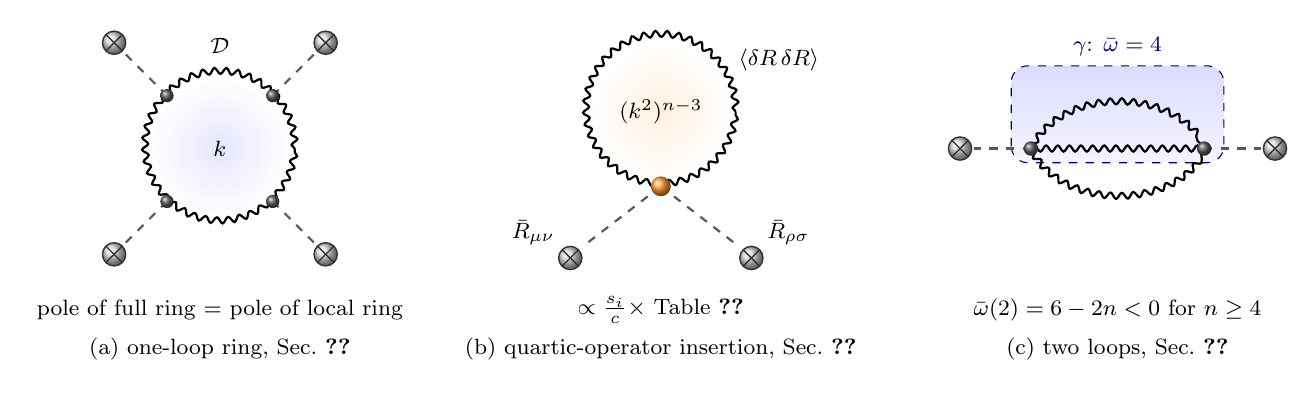
\begin{tikzpicture}[font=\footnotesize]
\tikzset{otimes/.pic={\shade[ball color=gray!30] (0,0) circle (4.2pt); \draw[gray!40!black,line width=0.5pt] (0,0) circle (4.2pt) (-2.97pt,-2.97pt) -- (2.97pt,2.97pt) (-2.97pt,2.97pt) -- (2.97pt,-2.97pt);}}
\begin{scope}[shift={(0,0)}]
  \shade[inner color=blue!10, outer color=white] (0,0) circle (0.9);
  \draw[grav] (0,0) circle (0.95);
  \foreach \ang in {45,135,225,315} {
    \draw[bkg] (\ang:0.95) -- (\ang:1.72);
    \pic at (\ang:1.9) {otimes};
    \shade[ball color=black!65] (\ang:0.95) circle (2.4pt);
  }
  \node at (0,0) {$k$};
  \node at (90:1.3) {$\mathcal D$};
  \node at (0,-2.55) {(a) one-loop ring, Sec.~\ref{sec:poles1}};
  \node[align=center] at (0,-2.05) {pole of full ring $=$ pole of local ring};
\end{scope}
\begin{scope}[shift={(5.6,-0.15)}]
  \shade[inner color=orange!12, outer color=white] (0,0.62) circle (0.9);
  \draw[grav] (0,0.62) circle (0.95);
  \draw[bkg] (0,-0.33) -- (-1.0,-1.1); \pic at (-1.15,-1.24) {otimes}; \node at (-1.62,-0.92) {$\bar R_{\mu\nu}$};
  \draw[bkg] (0,-0.33) -- (1.0,-1.1); \pic at (1.15,-1.24) {otimes}; \node at (1.62,-0.92) {$\bar R_{\rho\sigma}$};
  \shade[ball color=orange!80] (0,-0.33) circle (3.6pt);
  \node at (0,0.62) {$(k^2)^{n-3}$};
  \node at (1.5,1.27) {$\langle\delta R\,\delta R\rangle$};
  \node at (0,-2.4) {(b) quartic-operator insertion, Sec.~\ref{sec:killers}};
  \node[align=center] at (0,-1.9) {$\propto\frac{s_i}{c}\times$ Table~\ref{tab:killers}};
\end{scope}
\begin{scope}[shift={(11.4,0)}]
  \coordinate (L) at (-1.1,0); \coordinate (R) at (1.1,0);
  \begin{scope}[on background layer]
    \shade[top color=blue!14, bottom color=blue!4, rounded corners=6pt] (-1.35,-0.18) rectangle (1.35,1.05);
    \draw[blue!50!black, dashed, rounded corners=6pt] (-1.35,-0.18) rectangle (1.35,1.05);
  \end{scope}
  \draw[grav] (L) to[bend left=62] (R);
  \draw[grav] (L) -- (R);
  \draw[grav] (L) to[bend right=62] (R);
  \draw[bkg] (L) -- ++(-0.72,0); \pic at (-2.0,0) {otimes};
  \draw[bkg] (R) -- ++(0.72,0); \pic at (2.0,0) {otimes};
  \shade[ball color=black!65] (L) circle (2.6pt); \shade[ball color=black!65] (R) circle (2.6pt);
  \node[blue!50!black] at (0,1.3) {$\gamma$: $\bar\omega=4$};
  \node at (0,-2.55) {(c) two loops, Sec.~\ref{sec:degree}};
  \node[align=center] at (0,-2.05) {$\bar\omega(2)=6-2n<0$ for $n\ge4$};
\end{scope}
\end{tikzpicture}
\caption{Graphs behind the argument. Wavy lines are quantum gravitons (or ghosts), dashed lines end on background insertions $\otimes$. (a) A one-loop ring contributing to $\Gamma_1[\bar g]$. Replacing any vertex or propagator by its nonlocal remainder lowers the degree by at least $2n$, so the ultraviolet pole is that of the local theory. (b) The insertion of a quartic operator with two background curvatures: the loop of $(-\Box)^{n-3}$ between two linearized curvatures has an integrand $\propto k^{-4}$ and gives the poles of Table~\ref{tab:killers}. (c) A two-loop graph. The graph as a whole is convergent for $n\ge4$; the shaded one-loop subgraph $\gamma$ has degree $4$ and is the only possible source of a subdivergence.}
\label{fig:diagrams}
\end{figure*}

\section{Finiteness at all orders}
\label{sec:finite}

Assume A1 and A2, let $n\ge4$ be an integer, and choose $s_1,s_2,s_3$ as in Eq.~\eqref{eq:tuning}, with $c=c_\Pi$ the leading coefficient of the realization, Eq.~\eqref{eq:cone-real}. Then, for almost every realization of the gas, in dimensional regularization:
\begin{enumerate}[label=\textup{(\roman*)},leftmargin=2.2em,itemsep=0.2em]
\item The one-loop background-field effective action $\Gamma_1[\bar g]$ has no ultraviolet pole. This is Eq.~\eqref{eq:Gamma1} with the coefficients $\beta_i^{(0)}+\Delta\beta_i=0$ of Eqs.~\eqref{eq:killcontrib} and \eqref{eq:tuning}.
\item Every graph with two or more loops, and every subgraph with two or more loops, is ultraviolet convergent; the only subdivergences are those of one-loop subgraphs. This is Sec.~\ref{sec:degree} with $n\ge4$.
\item No coupling of the gauge-invariant action is renormalized at any order: not Newton's constant, not the cosmological constant, not $M$, $n$ or the $s_i$. Both constants receive finite one-loop shifts, which can be computed (Sec.~\ref{sec:vacuum}). The $S$ matrix is ultraviolet finite to all orders.
\end{enumerate}
The argument for (iii) is as follows. Consider the full effective action $\Gamma[\bar g,Q]$, with $Q$ the expectation values of the quantum fields and ghosts, and with sources for their BRST variations. By (ii) and the forest structure of dimensional regularization~\cite{Collins1984}, all counterterms are fixed by one-loop poles; no new counterterm is needed at higher loops, because there is no overall divergence there. The one-loop poles are local. Section~\ref{sec:poles1} shows that they equal those of the local theory, for graphs with background and with quantum external legs alike, and by the Slavnov--Taylor identity and the cohomological classification of Ref.~\cite{BarnichBrandtHenneaux2000}, applied to the local theory, the one-loop counterterm is the sum of a gauge-invariant functional of the full metric $\bar g+\kappa Q$ and a BRST-exact part. The gauge-invariant part has four derivatives and no dimensionful constant (Sec.~\ref{sec:form}), so it is $\beta_1R^2+\beta_2\Ric^2+\beta_EE$ of the full metric, fixed by its value at $Q=0$, which vanishes by (i). Only the BRST-exact part remains. It renormalizes the quantum fields, the ghosts and the gauge-fixing sector, and it is needed to subtract the subdivergences of off-shell subgraphs at two loops and beyond. A BRST-exact counterterm is a change of the gauge-fixing fermion, and such a change alters the background-field effective action only by terms proportional to its own equations of motion~\cite{KalloshTarasovTyutin1978,BarnichBrandtHenneaux2000}. The $S$ matrix, which is built from $\Gamma[\bar g]$ by tree graphs~\cite{AbbottGrisaruSchaefer1983}, is therefore unaffected, and no physical coupling receives a counterterm. The tuning~\eqref{eq:tuning} is made once, at one loop, and is not disturbed later, because at higher loops there is nothing to disturb it.

Table~\ref{tab:divergences} lists every kind of divergence that can arise, with its fate. The ultraviolet ones are removed: the dimensionful ones by saturation, the one-loop dimensionless ones by the quartic operators, and the higher-loop ones by power counting. What remains are the renormalizations of the gauge-fixing sector, which have no effect on observables, and the infrared divergences of on-shell amplitudes with soft gravitons. The latter are physical. They are those of general relativity, since $a=1+O(p^4/M^4)$ at small momentum, and they cancel in inclusive rates by Weinberg's soft-graviton theorem~\cite{Weinberg1965}. No ultraviolet completion can or should remove them.

\subsection{No cutoff in the answer}
\label{sec:nocutoff}

``Finite'' means different things in quantum field theory, and the sense used here should be stated. In the usual procedure a divergent integral is cut off at a momentum $\Lambda$, the dependence on $\Lambda$ is absorbed into bare couplings, and $\Lambda$ is then sent to infinity while the bare couplings follow it. Nothing of that kind happens in the theory of the gas.

The bare couplings $G$, $M$, $n$ and $s_1,s_2,s_3$ are fixed numbers. None of them depends on the regulator, and none is adjusted as the regulator is removed. In dimensional regularization the $S$ matrix computed from the bare action~\eqref{eq:action} has a finite limit as $\epsilon\to0$, and that limit is the physical $S$ matrix. This follows from the argument for (iii). With the BRST-exact counterterms added, every subdivergence is subtracted and the result is finite; those counterterms do not change the $S$ matrix; so the $S$ matrix is the same with and without them. Dependence on the regulator survives only in off-shell Green functions of the quantum fields and ghosts, which are not observable.

The logarithm is the only divergence of a one-loop integral that takes the same form in every regularization. Its coefficient is the residue of the pole in dimensional regularization, a local functional, and the tuning~\eqref{eq:tuning} sets it to zero. A regularization with a momentum cutoff produces, in addition, terms growing like $\Lambda^4$ and $\Lambda^2$ in front of $\int\sqrt g$ and $\int\sqrt g\,R$. Their coefficients change when the shape of the cutoff is changed, and they are absent in dimensional regularization and in every other analytic regularization~\cite{Collins1984}. They carry no information about the theory. The finite remainder does, and the next subsection shows on the simplest example that it is the same for every regulator.

\subsection{The zero-point energy of the graviton}
\label{sec:vacuum}

The absence of a pole in $\int\sqrt{\bar g}$ does not mean that the one-loop effective action has no such term. It has a finite one, and it can be computed exactly. On flat space $\Gamma_1=(\rho_1+\delta\rho_\Pi)\int\dd^4x$, where $\rho_1+\delta\rho_\Pi$ is the zero-point energy density of the graviton together with the ghosts and the compensating factor of Sec.~\ref{sec:gf}; $\rho_1$ comes from the skeleton and $\delta\rho_\Pi$ from the fluctuation $R_\Pi$ of the realization. Around flat space the graviton operator is $p^2a(p^2)(\mathbf 1-\frac12\delta\otimes\delta)$ on the ten components of $h_{\mu\nu}$, the ghost operator is $p^2a(p^2)\,\delta_{\mu\nu}$ on four components, and the compensating factor is $\frac12\Tr\log a$ on four components. A real bosonic component contributes $\frac12\log$ of its eigenvalue and a ghost--antighost pair contributes $-\log$, so per momentum the integrand is
\begin{equation}
\label{eq:count}
5\log(p^2a)-4\log(p^2a)+2\log a=\log p^2+3\log a,
\end{equation}
up to a constant from $\det(\mathbf 1-\frac12\delta\otimes\delta)$ that, like $\int\dd^Dk$ of any constant, vanishes in dimensional regularization. The same integrand follows without gauge fixing. The six transverse components of $h_{\mu\nu}$ each contribute $\frac12\log(p^2a)$, and the Jacobian of the split of $h_{\mu\nu}$ into its transverse part and a gauge orbit contributes $-2\log p^2$, with no factor of $a$. The coefficient $3$ of $\log a$ is therefore independent of the gauge.

The first term in Eq.~\eqref{eq:count} is that of general relativity. Its integral $\int\dd^Dk\,\log k^2$ has no scale and vanishes in dimensional regularization. The second term is $3\log a=\frac{3n}2\Ein(k^4/M^4)+3R_\Pi(k^2)$, by Eq.~\eqref{eq:split}. We take the skeleton part first. With $w=k^4/M^4$ and $\Omega_D=2\pi^{D/2}/\Gamma(D/2)$ the area of the unit sphere,
\[
\int\dd^Dk\,\Ein\Bigl(\frac{k^4}{M^4}\Bigr)=\frac{\Omega_DM^D}4\int_0^\infty w^{D/4-1}\,\Ein(w)\,\dd w .
\]
The last integral is a Mellin transform, and for $\Ein$ it is elementary. For $-1<\mathrm{Re}\,s<0$ one has $\int_0^\infty w^{s-1}(1-e^{-wt})\,\dd w=-\Gamma(s)\,t^{-s}$. Integrating over $t\in[0,1]$ with the weight $\dd t/t$, as in the definition of $\Ein$, gives
\begin{equation}
\label{eq:mellin}
\int_0^\infty w^{s-1}\,\Ein(w)\,\dd w=\frac{\Gamma(s)}{s},\qquad -1<\mathrm{Re}\,s<0 .
\end{equation}
The strip is where the integral converges, since $\Ein(w)\simeq w$ at small $w$ and $\Ein(w)\simeq\log w$ at large $w$. Dimensional regularization defines the radial integral by continuation in $D$~\cite{Collins1984}, that is in $s=D/4$, and the right side of Eq.~\eqref{eq:mellin} is meromorphic with poles only at $s=0,-1,-2,\dots$. At $D=4$, that is $s=1$, it is regular and equals $\Gamma(1)=1$. Hence $\int\dd^4k\,(2\pi)^{-4}\,\Ein(k^4/M^4)=2\pi^2M^4/(4\cdot16\pi^4)=M^4/(32\pi^2)$, and
\begin{equation}
\label{eq:rho}
\rho_1=\frac{3n}{2}\,\frac{M^4}{32\pi^2}=\frac{3n\,M^4}{64\pi^2}.
\end{equation}
There is no pole, as Sec.~\ref{sec:form} requires, and the value is positive. In the normalization of Eq.~\eqref{eq:action}, where a cosmological term enters as $-\frac2{\kappa^2}\int\sqrt g\,(-2\Lambda)$, Eq.~\eqref{eq:rho} is a finite cosmological constant $\Lambda_1=\frac{\kappa^2}4\rho_1=3nGM^4/(8\pi)$. For a general admissible response the second term of Eq.~\eqref{eq:count} is $3n\Phi(k^2/M^2)$, and Eq.~\eqref{eq:moment} gives
\begin{equation}
\label{eq:rho-gen}
\rho_1=\frac{3nM^4}{32\pi^2}\,\mu_\psi=\frac{3nM^4}{32\pi^2}\int_0^\infty t\,\bigl(1-\psi(t)\bigr)\,\dd t ,
\end{equation}
positive and finite for every response that saturates; Table~\ref{tab:class} lists three values.

The fluctuation term is the realization's own contribution. In dimensional regularization the integral of the constant $R_\infty$ vanishes, and what is left, $R_\Pi-R_\infty$, falls along the Euclidean axis like $k^{-\sigma+2\varepsilon}$ by Eq.~\eqref{eq:asdecay}, faster than $k^{-4}$, so its integral converges absolutely and is the same in every regularization. Inserting Eq.~\eqref{eq:fdef} and integrating brane by brane with Eq.~\eqref{eq:moment1},\footnote{The exchange of the momentum integral and the compensated sum is justified by truncation. For the branes larger than $\eta/M^2$ the sum is finite and the exchange is trivial. As $\eta\to0$ the right side of Eq.~\eqref{eq:drho} converges in mean square by Eq.~\eqref{eq:isometry}, and so does the left side, by Minkowski's inequality: the root-mean-square difference at momentum $k$ is at most $[nV(\eta)]^{1/2}$ and, by Eq.~\eqref{eq:msdecay}, at most $C|k|^{-\sigma}$ for large $k$, which is integrable.}
\begin{equation}
\label{eq:drho}
\begin{aligned}
\delta\rho_\Pi&=3\int\frac{\dd^4k}{(2\pi)^4}\bigl[R_\Pi(k^2)-R_\infty\bigr]\\
&=-\frac{3M^4\mu_\psi}{16\pi^2}\int\frac{\vartheta(s)}{(sM^2)^2}\,(\Pi-\nu)(\dd s).
\end{aligned}
\end{equation}
This is a compensated sum over the branes, with mean zero and, by Eq.~\eqref{eq:isometry}, variance $(3M^4\mu_\psi/16\pi^2)^2\,n\int_0^1\vartheta(\tau)\tau^{-4}\dd\tau/\tau$. The integral converges when $V(t)=O(t^\sigma)$ with $\sigma>4$, which (G) guarantees. For the power law~\eqref{eq:finegrain} the variance is $(3M^4\mu_\psi/16\pi^2)^2\,n\vartheta_0/(\zeta-4)$, and relative to the mean~\eqref{eq:rho-gen} the standard deviation is
\begin{equation}
\label{eq:drhorel}
\frac{(\bE\,\delta\rho_\Pi^2)^{1/2}}{\rho_1}=2\Bigl[\frac{\vartheta_0}{n(\zeta-4)}\Bigr]^{1/2},
\end{equation}
independent of the response. Table~\ref{tab:fluct} gives $0.37$ for $n=4$ and $\zeta=9$, and $0.83$ for $\zeta=5$. The zero-point energy of a realization is therefore $\rho_1+\delta\rho_\Pi$, a finite number that is the same for every regulator, whose mean over realizations is Eq.~\eqref{eq:rho-gen}. Each brane lowers it, by an amount proportional to $\vartheta(s)/s^2$; the positive mean is the dimensionally continued sum over the infinitely many small branes, $\int_0^1\tau^{-2}\,\dd\tau/\tau=-\frac12$ by continuation, which is how a sum of negative terms acquires the positive value~\eqref{eq:rho}.

The number in Eq.~\eqref{eq:rho} is not a property of dimensional regularization. Cut the radial integral off at $w=W$, that is at $k=\Lambda$ with $W=\Lambda^4/M^4$. Integrating by parts with $\Ein'(w)=(1-e^{-w})/w$ and using Eq.~\eqref{eq:Ein-E1},
\begin{align*}
\int_0^W\Ein(w)\,\dd w&=W\Ein(W)-W+1-e^{-W}\\
&=W\log W+(\gE-1)W+1+O(e^{-W}).
\end{align*}
With a smooth cutoff the same integral is
\begin{align*}
\int_0^\infty\Ein(w)\,e^{-w/W}\,\dd w&=W\log(1+W)\\
&=W\log W+1+O(W^{-1}),
\end{align*}
because $\int_0^\infty e^{-w/W}(1-e^{-wt})\,\dd w=W^2t/(1+Wt)$ and $\int_0^1W^2\,\dd t/(1+Wt)=W\log(1+W)$. The terms that grow with $W$, of order $\Lambda^4\log(\Lambda/M)$ and $\Lambda^4$, differ between the two cutoffs. The constant is $1$ in both, the value of $\Gamma(s)/s$ at $s=1$, and this is true for any cutoff function.\footnote{Let $r$ be smooth on $[0,\infty)$ and rapidly decreasing, with $r(0)=1$, and let $\tilde r(s)=\int_0^\infty u^{s-1}r(u)\,\dd u$. By the Mellin--Parseval formula, $\int_0^\infty\Ein(w)\,r(w/W)\,\dd w=\frac1{2\pi i}\int_{\mathrm{Re}\,s=s_0}\frac{\Gamma(s)}s\,\tilde r(1-s)\,W^{1-s}\,\dd s$ with $-1<s_0<0$. Move the contour to the right. The double pole of $\Gamma(s)/s$ at $s=0$ gives the terms $W\log W$ and $W$, whose coefficients involve $\tilde r(1)$ and $\tilde r'(1)$ and so depend on the cutoff. The simple pole of $\tilde r(1-s)$ at $s=1$, where $\tilde r(1-s)\simeq r(0)/(1-s)$, gives the constant $\Gamma(1)\,r(0)=1$ for every $r$. What remains decays as a negative power of $W$.} The power-law terms are the scheme artifacts of Sec.~\ref{sec:nocutoff}; the finite part is universal. Figure~\ref{fig:vacuum} shows both halves of the argument: the Mellin transform with its strip of convergence and its value at $s=1$, and the remainder after the growing terms are removed, for a one-parameter family of cutoffs that ends in the sharp one.

\textit{Why the exponent in (G) is $4$.} The fluctuation~\eqref{eq:drho} used (G) as a sufficient condition. It is also necessary, up to factors that vary more slowly than any power, and the reason is dimensional. A brane of size $s$ changes the zero-point energy by
\[
g(\tau)=-K\,\frac{\vartheta(\tau)}{\tau^2},\qquad K=\frac{3M^4\mu_\psi}{16\pi^2},\qquad\tau=sM^2,
\]
an energy density set by its own scale, and the variance of the sum over the gas adds the squares of these changes, $\int g^2\,\dd\nu=K^2n\int\vartheta\,\tau^{-4}\,\dd\tau/\tau$. The fourth power is the dimension of an energy density. Every regulator removes the branes too small to be resolved. Removing those smaller than $\eta/M^2$ leaves the compensated sum $X_\eta=\int_{\tau>\eta}g\,\dd(\Pi-\nu)$, and the zero-point energy of the realization is its limit as $\eta\to0$. The limit exists, almost surely, if and only if
\begin{equation}
\label{eq:necessity}
n\int_0^1\min\Bigl(\frac{\vartheta(\tau)}{\tau^{4}},\,\frac1{\tau^{2}}\Bigr)\frac{\dd\tau}\tau<\infty ,
\end{equation}
and when the integral diverges $X_\eta$ has no limit even in distribution.\footnote{The increments of $X_\eta$ over disjoint ranges of size are independent, and Eq.~\eqref{eq:pgfl} with $f=e^{iug}-1$ gives $|\bE\,e^{iuX_\eta}|=\exp\int_{\tau>\eta}[\cos(ug)-1]\,\dd\nu$. The average of $1-\cos(ug)$ over $u\in[-h,h]$ is $1-\sin(hg)/(hg)$, which is at least $\frac1{10}\min(1,h^2g^2)$. If $\int\min(1,g^2/K^2)\,\dd\nu=\infty$, the average of $-\log|\bE\,e^{iuX_\eta}|$ over $[-h,h]$ therefore diverges as $\eta\to0$, for every $h>0$. A limit in distribution is excluded, because its characteristic function would equal $1$ at $u=0$, be continuous there, and be the uniform limit of those of $X_\eta$ on $[-h,h]$~\cite{Feller1971}. If $\int\min(1,g^2/K^2)\,\dd\nu<\infty$, split the branes at $|g|=K$. Those with $|g|\le K$ give a compensated sum with $\int g^2\,\dd\nu<\infty$, which converges as in Sec.~\ref{sec:avg}. Those with $|g|>K$ have a finite expected number, so almost surely there are finitely many and their sum converges; their compensator $\int_{\tau>\eta,\,|g|>K}g\,\dd\nu$ converges if and only if $\int_{|g|>K}|g|\,\dd\nu<\infty$, because $g$ has one sign, and otherwise $X_\eta\to+\infty$. The two conditions together are Eq.~\eqref{eq:necessity}, since $g^2\,\dd\nu=K^2n\vartheta\tau^{-4}\,\dd\tau/\tau$ and $|g|\,\dd\nu=Kn\tau^{-2}\,\dd\tau/\tau$.} For a gas in which smaller branes are never stronger, $\vartheta$ nondecreasing, Eq.~\eqref{eq:necessity} is equivalent to
\begin{equation}
\label{eq:necessityV}
\int_0^1V(\tau)\,\tau^{-5}\,\dd\tau<\infty .
\end{equation}
This requires $V(t)=o(t^4)$, and (G) implies it.\footnote{If $\vartheta$ is nondecreasing, the part of the integral~\eqref{eq:necessity} over $[t/2,t]$ is at least $n\log2\,\min\bigl(\vartheta(t/2)\,t^{-4},t^{-2}\bigr)$ and tends to zero with $t$, so $\vartheta(\tau)=o(\tau^4)$ and the minimum is $\vartheta\tau^{-4}$ near $\tau=0$. Since $\dd V=\vartheta\,\dd\tau/\tau$, Eq.~\eqref{eq:necessity} then reads $\int_0^1\tau^{-4}\,\dd V<\infty$. As $V(t)\,t^{-4}\le\int_0^t\tau^{-4}\,\dd V$, which tends to zero, integration by parts gives $\int_0^1\tau^{-4}\,\dd V=V(1)+4\int_0^1V\tau^{-5}\,\dd\tau$. Conversely $\int_t^{2t}V\tau^{-5}\,\dd\tau\ge\frac{15}{64}V(t)\,t^{-4}$, so Eq.~\eqref{eq:necessityV} forces $V(t)\,t^{-4}\to0$ and the integration by parts runs backwards; since the minimum in Eq.~\eqref{eq:necessity} is at most $\vartheta\tau^{-4}$, this direction needs no monotonicity. Under (G), $\int_0^1V\tau^{-5}\,\dd\tau\le C/(\sigma-4)$.} The two differ only by profiles that approach $t^4$ more slowly than any power, such as $V(t)=t^4/\log^2(1/t)$, which satisfies Eq.~\eqref{eq:necessityV} but not (G). For the power law~\eqref{eq:finegrain} both hold exactly when $\zeta>4$.

A momentum cutoff shows the same threshold, and shows what goes wrong below it. With $|k|<\Lambda$ a brane contributes $g(\tau)\,\mu(\tau\Lambda^2/M^2)/\mu_\psi$ instead of $g(\tau)$, where $\mu(U)=\int_0^Uu\,[1-\psi(u)]\,\dd u$ rises from $0$ to $\mu_\psi$. For the power law and $\psi_*$ the realization's part of the regulated zero-point energy, $\delta\rho_\Lambda$, has mean zero and, for $0<\zeta<4$ and $\Lambda\gg M$, the variance
\begin{equation}
\label{eq:cutvar}
\begin{gathered}
\bE\,\delta\rho_\Lambda^2\simeq K^2n\vartheta_0\,C_\zeta\Bigl(\frac\Lambda M\Bigr)^{2(4-\zeta)},\\
C_\zeta=\tfrac12\,\Gamma\bigl(\tfrac\zeta2-2\bigr)\bigl(2^{\,2-\zeta/2}-2\bigr),
\end{gathered}
\end{equation}
which at $\zeta=4$ grows like $2K^2n\vartheta_0\log(\Lambda/M)$ and for $\zeta>4$ tends to the variance $K^2n\vartheta_0/(\zeta-4)$ of Eq.~\eqref{eq:drho}.\footnote{By Eq.~\eqref{eq:isometry} the variance is $\int g^2\,[\mu(\tau\Lambda^2/M^2)/\mu_\psi]^2\,\dd\nu$. For $\psi_*$, $\mu(U)/\mu_\psi=1-e^{-U^2}$, and the substitution $\tau=vM^2/\Lambda^2$ turns the variance into $K^2n\vartheta_0(\Lambda/M)^{2(4-\zeta)}\int_0^{\Lambda^2/M^2}v^{\zeta-5}(1-e^{-v^2})^2\,\dd v$. For $0<\zeta<4$ the integral converges as $\Lambda\to\infty$. With $u=v^2$ and $\int_0^\infty u^{s-1}(1-e^{-u})^2\,\dd u=\Gamma(s)\,(2^{-s}-2)$, which follows from $\int_0^\infty u^{s-1}(e^{-bu}-1)\,\dd u=b^{-s}\Gamma(s)$ for $-1<\mathrm{Re}\,s<0$ and extends to $-2<\mathrm{Re}\,s<0$ by continuation, it equals $C_\zeta$. At $\zeta=2$ the formula is read as its limit, $C_2=\log2$, and $C_\zeta\simeq1/(4-\zeta)$ as $\zeta\to4$. For $\zeta>4$ the integral grows like $(\Lambda/M)^{2(\zeta-4)}/(\zeta-4)$, and the product tends to $K^2n\vartheta_0/(\zeta-4)$.} Under Eq.~\eqref{eq:necessity} every cutoff, on momenta or on sizes and of any shape, converges to the same $\delta\rho_\Pi$.\footnote{A cutoff of shape $r$ on momenta, with $0\le r\le1$ and $r(0)=1$, replaces $g$ by $g\,m_r(\tau\Lambda^2/M^2)$, where $m_r(U)=\mu_\psi^{-1}\int_0^\infty u\,[1-\psi(u)]\,r(u/U)\,\dd u$ lies in $[0,1]$ and tends to $1$ as $U\to\infty$. A cutoff on sizes replaces it by $g$ times the indicator of $\tau>\eta$. In both cases the modified contribution is bounded by $|g|$ and tends to $g$ brane by brane. Split the branes at $|g|=K$. For those with $|g|\le K$ the compensated sums converge in mean square, by Eq.~\eqref{eq:isometry} and dominated convergence; those with $|g|>K$ are finitely many, and their compensator converges by dominated convergence.} Without it the regulated value of a realization contains a random term whose spread grows like $(\Lambda/M)^{4-\zeta}$ and which has no limit, by the argument of the footnote to Eq.~\eqref{eq:necessity}. A term that grows with the cutoff and has a fixed coefficient is a scheme artifact of the kind discussed in Sec.~\ref{sec:nocutoff}, and it changes in a known way when the regulator changes. This one differs from realization to realization, two cutoffs of different shape disagree about it by an amount whose spread grows in the same way, and the bare cosmological constant could absorb it only by being readjusted for each realization and each cutoff, without a limit. The zero-point energy then has no value that is the same for every regulator. Condition (G) is what keeps the finite answer of this section, and the exponent in it is the dimension of the quantity computed. Figure~\ref{fig:necessity} shows the threshold.

In general relativity the zero-point integrand is $\log k^2$ alone. Its integral is zero in dimensional regularization and quartic with a cutoff, and it has no finite part that is independent of the regulator. In the theory of the gas the form factor turns it into a definite number set by $M$, $n$ and the realization. Newton's constant receives a finite shift of the same kind, proportional to $M^2$, which we have not computed. The cosmological constant is then the sum of a bare term, which is not renormalized, and $\Lambda_1$. Making the total small is still a choice of the bare term, but it is now a choice between two finite numbers rather than the subtraction of a divergence, and the theory does not explain why the total is small. Matter fields, which this paper does not include, would add zero-point energies of their own.

\begin{figure*}[t]
\centering
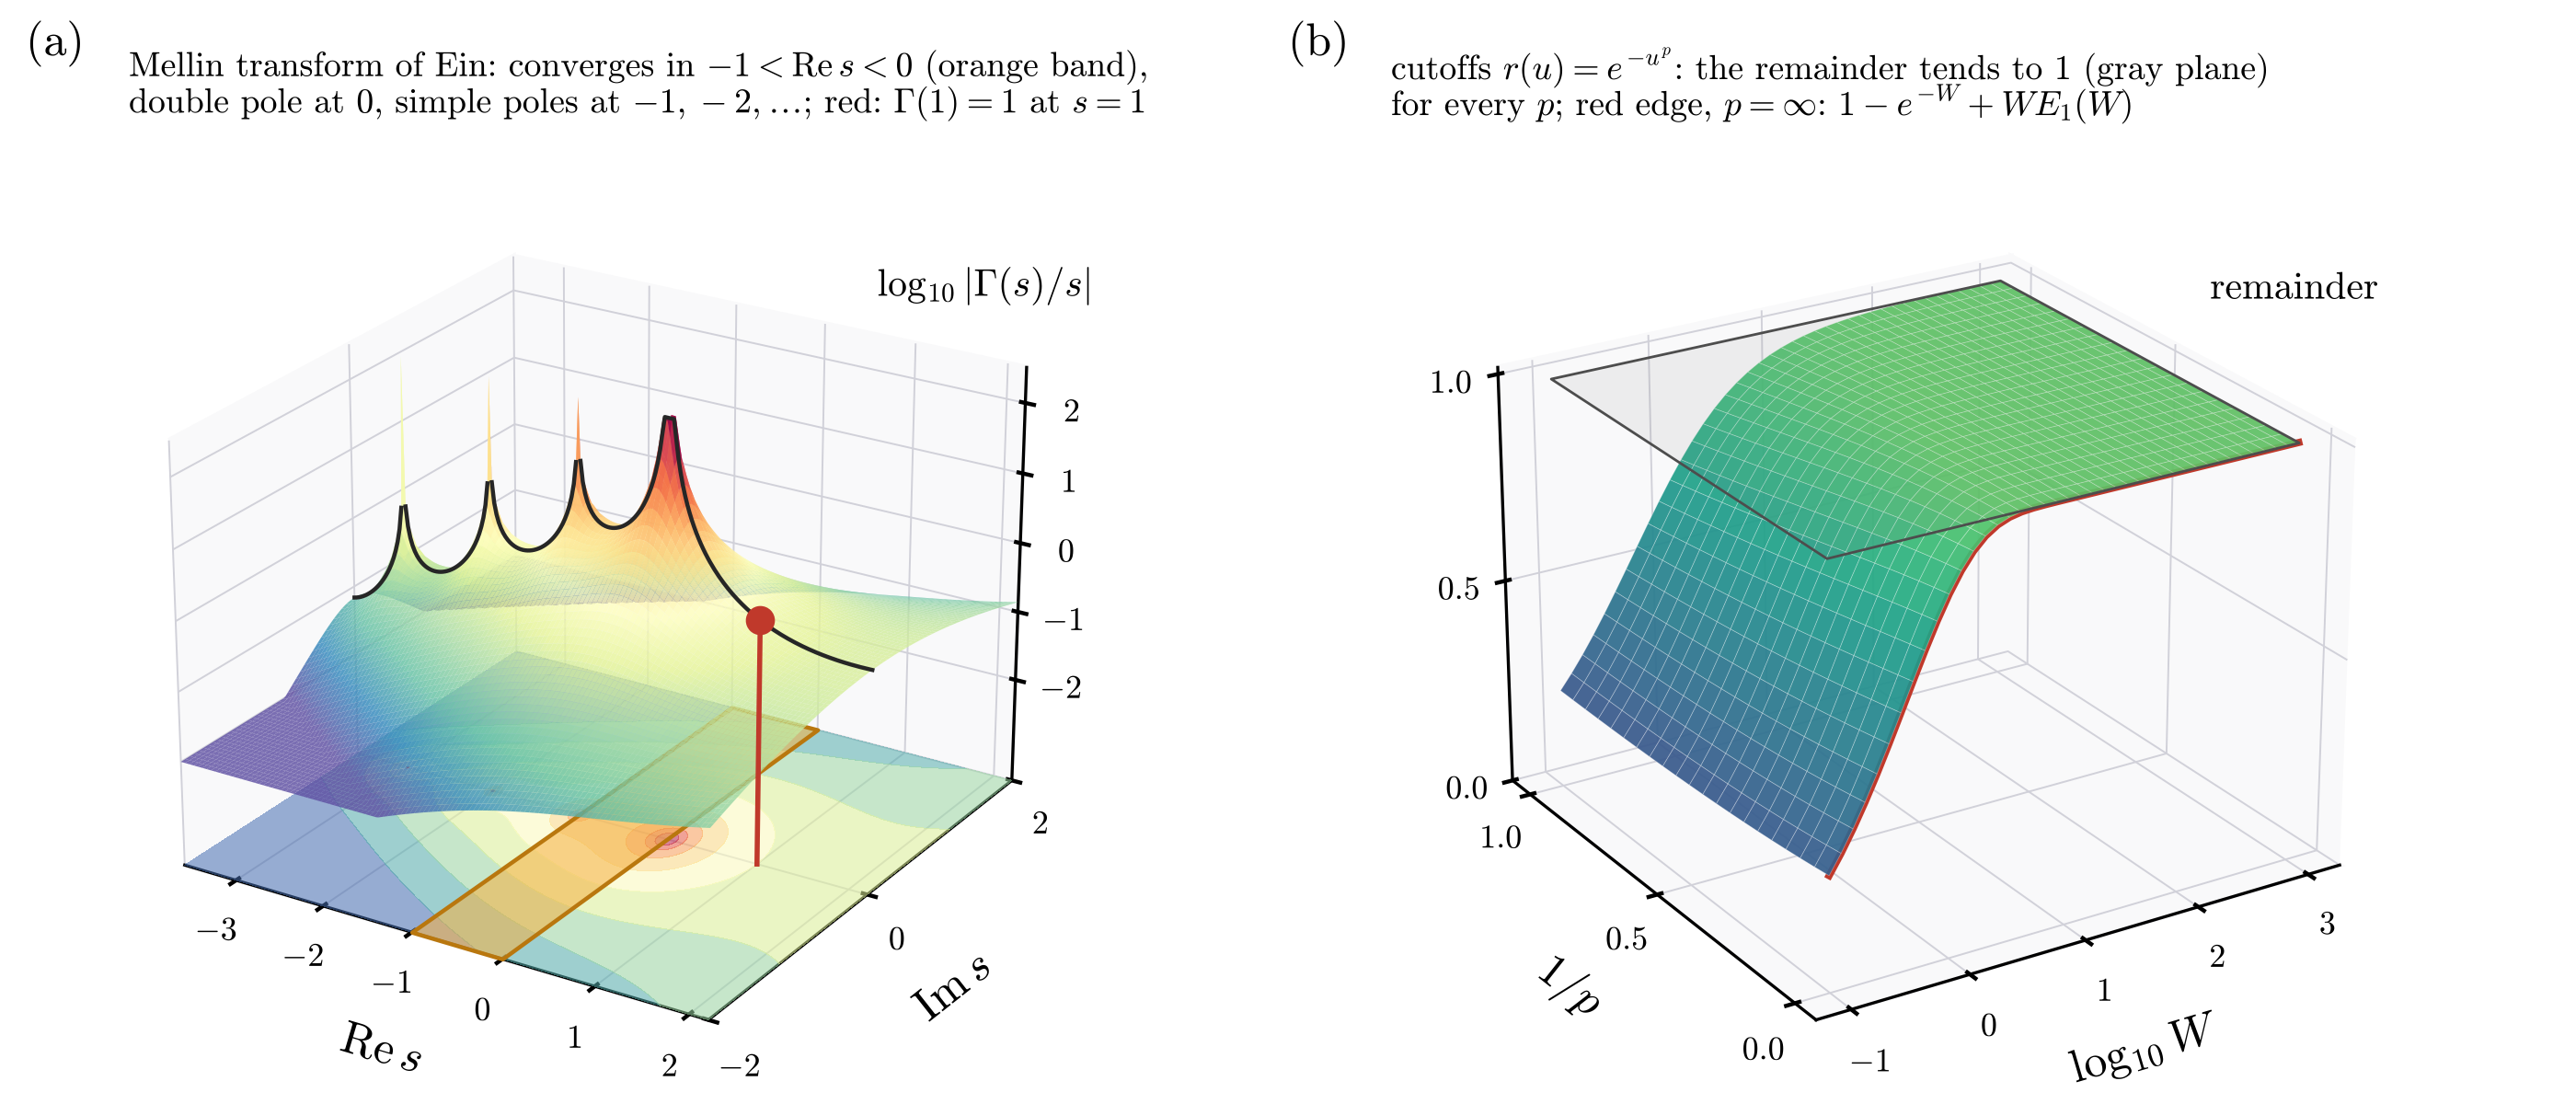
\includegraphics[width=\textwidth]{figs/fig_vacuum.png}
\caption{The finite zero-point energy. (a) $\log_{10}|\Gamma(s)/s|$ over the complex $s$ plane, the Mellin transform~\eqref{eq:mellin} of $\Ein$. The integral converges in the strip $-1<\mathrm{Re}\,s<0$ (orange band on the floor, which also carries the contours of the surface); its continuation has a double pole at $s=0$ and simple poles at $s=-1,-2,\dots$ (black curve along the real axis), and is regular at $s=1$, where it equals $1$ (red). That value is the whole answer~\eqref{eq:rho}. (b) The integral $\int_0^\infty\Ein(w)\,r(w/W)\,\dd w$ with the cutoffs $r(u)=e^{-u^p}$, after the terms that grow with $W$ are subtracted, $\tilde r(1)\,W\log W+[\tilde r'(1)+\gE\tilde r(1)]\,W$, with $\tilde r$ the Mellin transform of $r$. The surface is drawn over $\log_{10}W$ and $1/p\in[0,1]$. The coefficients of the subtracted terms depend on $p$, the remainder does not: it tends to $1$ (gray plane) for every $p$, and at $W=10^3$ it lies within $10^{-3}$ of $1$ across the whole family. The red edge $1/p=0$ is the sharp cutoff, where the remainder is $1-e^{-W}+W E_1(W)$.}
\label{fig:vacuum}
\end{figure*}

\begin{figure*}[t]
\centering
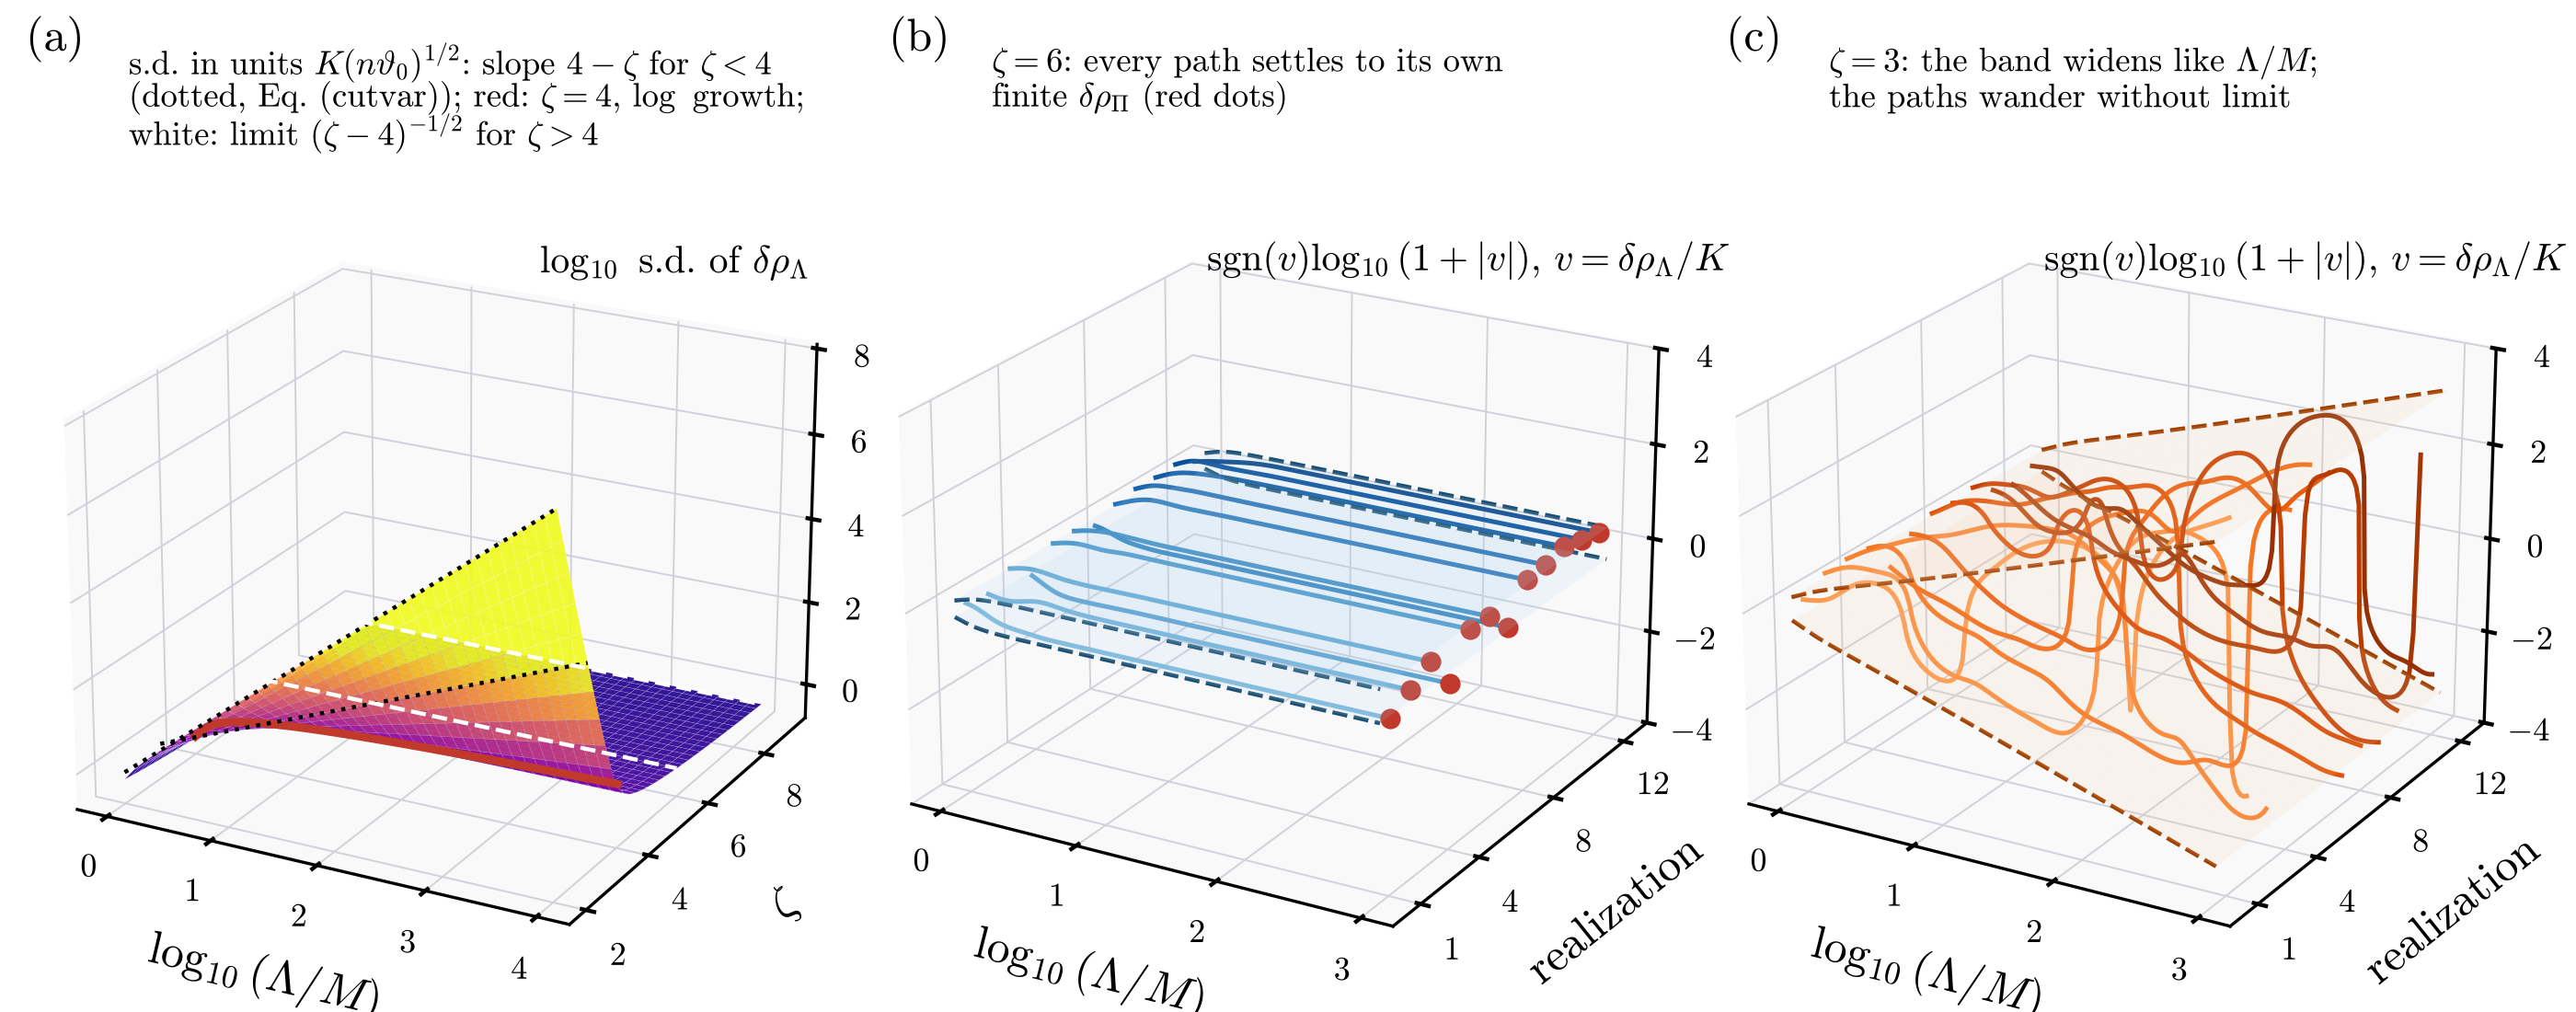
\includegraphics[width=\textwidth]{figs/fig_necessity.png}
\caption{Why condition (G) needs $\zeta>4$, for $n=4$, $\vartheta_0=\log2$, $\psi_*$ and a sharp momentum cutoff $\Lambda$. (a) The standard deviation of the realization's part $\delta\rho_\Lambda$ of the zero-point energy, in units of $K(n\vartheta_0)^{1/2}$, as a surface over $\log_{10}(\Lambda/M)$ and $\zeta$, in $\log_{10}$, computed from the exact integral in the footnote to Eq.~\eqref{eq:cutvar}. For $\zeta>4$ it levels off at $(\zeta-4)^{-1/2}$, the spread of the finite $\delta\rho_\Pi$ of Eq.~\eqref{eq:drho}; for $\zeta<4$ it grows with slope $4-\zeta$ (dotted lines, Eq.~\eqref{eq:cutvar}); the red curve is $\zeta=4$, where the growth is logarithmic. (b) Twelve realizations of $v=\delta\rho_\Lambda/K$ as functions of the cutoff for $\zeta=6$, on the compressed scale $\mathrm{sgn}(v)\log_{10}(1+|v|)$, with the band $\pm(\bE\,\delta\rho_\Lambda^2)^{1/2}/K$ (translucent sheet with dashed edges). Every path settles to its own finite value, marked by a dot. (c) The same for $\zeta=3$. The band widens like $\Lambda/M$ and the paths wander without limit, so the zero-point energy of a realization depends on where the regulator is put. In (b) and (c) the branes smaller than $0.3\,M^{-2}$ are represented, shell by shell in $\log\tau$, by their Gaussian limit; the larger ones are drawn individually.}
\label{fig:necessity}
\end{figure*}

\section{Unitarity}
\label{sec:unitarity}

The spectrum of Sec.~\ref{sec:prop} is a statement about the tree-level propagator. Loops raise a separate question, because $1/a$ is unbounded near the imaginary $z$ axis, as Sec.~\ref{sec:closed} shows for the skeleton, and the loop energies cannot be Wick-rotated in the usual way. A theory with such a form factor has to be defined by a prescription. We use the one that goes back to Efimov~\cite{Efimov1967} and was put in its modern form by Pius and Sen~\cite{PiusSen2016}. Loop integrals are defined with Euclidean loop momenta. Lorentzian amplitudes are the analytic continuations of the Euclidean ones in the external energies, and during the continuation the contours of the loop energies are deformed to avoid the poles of the propagators while their end points stay at $\pm i\infty$. Figure~\ref{fig:unitarity}(a) shows why the end points matter: the propagator is small along the Euclidean contour and along the real axis away from its pole, and in the wedges between them it swings between very large and very small values.

The prescription is not one choice among several. The Euclidean amplitudes are finite and unambiguous (Sec.~\ref{sec:finite}), and they are analytic in the external momenta in a neighborhood of the Euclidean section, because the loop integrals converge absolutely and uniformly there. An analytic function has at most one continuation along a given path. Once the physical region is approached from the upper half plane of the external energies, the side fixed by the $+i0$ of local theories, the Lorentzian amplitude is therefore determined by the Euclidean one, and the contour deformation of Efimov, Pius and Sen is a construction of that continuation rather than an additional rule.\footnote{Pius and Sen show that the amplitude defined by the deformed contours is analytic in the external energies on the way from the Euclidean section to the physical region~\cite{PiusSen2016}. Any other definition that agrees with the Euclidean amplitude and is analytic on the same path coincides with it, by the identity theorem. A definition that differs must therefore either give up the Euclidean theory or give up analyticity in the external energies.} Definitions that start elsewhere do differ. Buoninfante compared three of them on the one-loop bubbles of a string-inspired scalar model and found that loop integrals written directly in Minkowski signature with Feynman's $i0$ diverge when the vertices are entire functions, because of their essential singularity at infinity, while the Schwinger proper-time definition agrees with the Euclidean one~\cite{Buoninfante2022}; the cell model of Sec.~\ref{sec:cells} is itself a statement about proper time. Section~\ref{sec:bubble} carries out the continuation for a one-loop bubble of the gas in closed form. It tests the cutting rule without the general argument, and it shows what the prescription implies for the size of amplitudes.

In this prescription the physical $S$ matrix is unitary at every order of perturbation theory. The proof has the two steps familiar from local gauge theories. First, the amplitudes obey the Cutkosky cutting rules with all ten components of the graviton and the ghosts on the cut lines, which is unitarity in the space of all asymptotic states, whose metric is indefinite (Sec.~\ref{sec:cutkosky}). Second, BRST invariance removes the states of negative and zero norm by the quartet mechanism of Kugo and Ojima (Sec.~\ref{sec:quartets}). Table~\ref{tab:unitarity} lists every input and where it is established.

\begin{figure*}[t]
\centering
\begin{minipage}[c]{0.47\textwidth}\centering
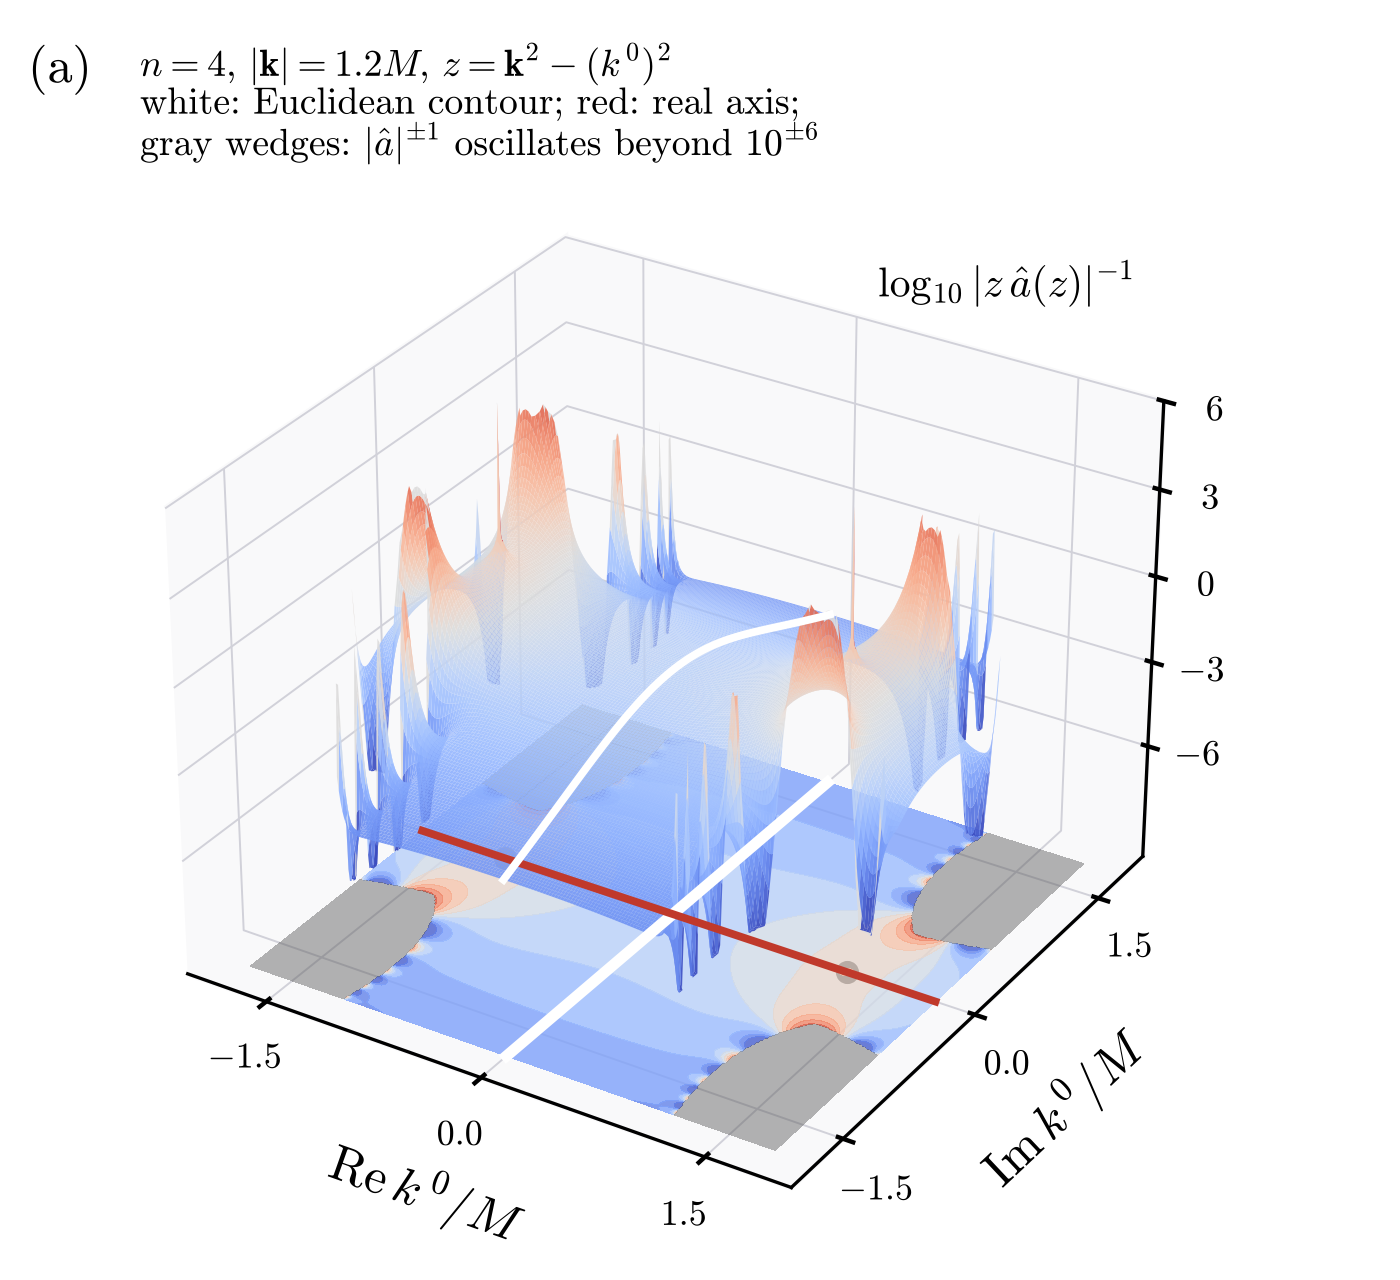
\includegraphics[width=\linewidth]{figs/fig_unitarity.png}
\end{minipage}\hfill
\begin{minipage}[c]{0.50\textwidth}\centering
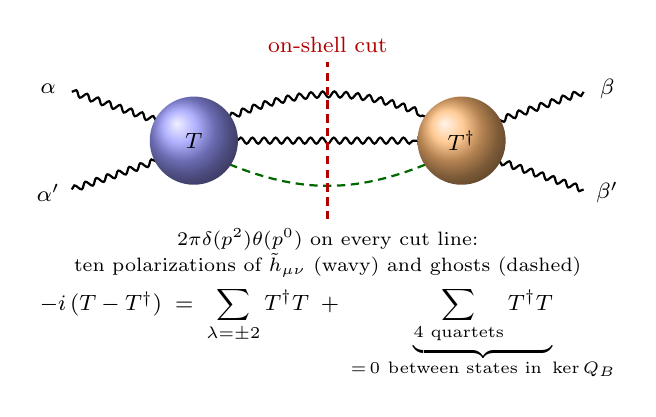
\begin{tikzpicture}[font=\footnotesize]
\draw[grav] (-1.55,0.62) -- (-0.48,0.26); \draw[grav] (-1.55,-0.62) -- (-0.48,-0.26);
\draw[grav] (4.95,0.62) -- (3.88,0.26); \draw[grav] (4.95,-0.62) -- (3.88,-0.26);
\node at (-1.85,0.66) {$\alpha$}; \node at (-1.85,-0.66) {$\alpha'$};
\node at (5.25,0.66) {$\beta$}; \node at (5.25,-0.66) {$\beta'$};
\draw[grav] (0.45,0.3) to[bend left=22] (2.95,0.3);
\draw[grav] (0.55,0) -- (2.85,0);
\draw[densely dashed,thick,green!40!black] (0.45,-0.3) to[bend right=22] (2.95,-0.3);
\shade[ball color=blue!40] (0,0) circle (0.56); \node at (0,0) {$T$};
\shade[ball color=orange!55] (3.4,0) circle (0.56); \node at (3.4,0) {$T^\dagger$};
\draw[red!70!black,very thick,dash pattern=on 3pt off 2pt] (1.7,-1.0) -- (1.7,1.0);
\node[red!70!black] at (1.7,1.22) {on-shell cut};
\node[align=center,font=\scriptsize] at (1.7,-1.42) {$2\pi\delta(p^2)\theta(p^0)$ on every cut line:\\ ten polarizations of $\tilde h_{\mu\nu}$ (wavy) and ghosts (dashed)};
\node at (1.7,-2.45) {$-i\,(T-T^\dagger)\;=\;\displaystyle\sum_{\lambda=\pm2}T^\dagger T\;+\;\underbrace{\sum_{\text{4 quartets}}T^\dagger T}_{=\,0\ \text{between states in }\ker Q_B}$};
\end{tikzpicture}
\end{minipage}
\caption{Unitarity in the Efimov--Pius--Sen prescription. (a) The size of a propagator, $\log_{10}|z\,\hat a(z)|^{-1}$ for the skeleton, over the complex plane of the loop energy $k^0$ at fixed spatial momentum $|\mathbf k|=1.2M$, for $n=4$, with $z=\mathbf k^2-(k^0)^2$. Along the Euclidean contour (white, $\mathrm{Re}\,k^0=0$, drawn on the floor and on the surface) and along the real axis away from the poles at $k^0=\pm|\mathbf k|$ (red, black dots) the propagator is small. In the wedges around $\arg k^0=\pm\pi/4,\pm3\pi/4$, where $z$ is close to the imaginary axis, $\log|\hat a|$ has an oscillating part of size $\frac n2|E_1(z^2/M^4)|$, which grows like $e^{|\mathrm{Re}\,z^2|/M^4}$, so the propagator swings between extremely large and extremely small values; this is why the loop energies cannot be rotated to the real axis. The surface is clipped at $\pm6$ and left out where that oscillating part exceeds $6$ decades (gray on the floor). (b) The cutting rule of Sec.~\ref{sec:cutkosky}: the anti-Hermitian part of an amplitude is the sum over cuts with all eighteen on-shell modes of the redefined fields. Between physical states, those in $\ker Q_B$, the contributions of the four BRST quartets cancel (Sec.~\ref{sec:quartets}), and only the two helicities of the graviton remain.}
\label{fig:unitarity}
\end{figure*}

\subsection{Cutting rules}
\label{sec:cutkosky}

Briscese and Modesto proved the Cutkosky rules for nonlocal theories whose form factor $e^{H}$ has the following four properties~\cite{BrisceseModesto2019}:
\begin{enumerate}[label=\textup{(U\arabic*)},leftmargin=2.4em,itemsep=0.15em]
\item $H$ is an entire function;
\item $e^{H}$ has no zeros and no poles at finite momentum;
\item $e^{H}$ grows without bound at the ends of the loop-energy contours and as the spatial loop momentum grows;
\item $H$ is asymptotically logarithmic in a cone around the real axis of the squared momentum.
\end{enumerate}
Their proof is written out for a scalar field with a local kinetic term, obtained by a field redefinition, and vertices that carry a factor $e^{-H/2}$ for every leg. It follows the proof of Pius and Sen for string field theory~\cite{PiusSen2016}, and Chin and Tomboulis reached the same cutting rule for general entire vertices by way of the Landau equations~\cite{ChinTomboulis2018}. In all three the Feynman rules enter through three properties only:\footnote{The Gaussian or exponential form of the vertices in Refs.~\cite{PiusSen2016,BrisceseModesto2019} is used to show that the integrals converge at the ends of the deformed contours, which is (P3). The rest of the argument, the continuation of the Euclidean amplitude into the physical region from the upper half plane of the external energies, the pinching of the contours at the poles of the propagators, and the identification of the anti-Hermitian part with the sum over cuts, uses only the location of the poles and the analyticity of the vertices.}
\begin{enumerate}[label=\textup{(P\arabic*)},leftmargin=2.4em,itemsep=0.15em]
\item the propagators are those of a local theory;
\item the vertices are entire functions of the momenta on their legs, with real Taylor coefficients in Euclidean variables;
\item on the deformed contours the integrand of every graph, together with its counterterms, is absolutely integrable at the ends of the contours, uniformly for external momenta in compact sets.
\end{enumerate}
We verify them for the gravitational theory of the gas.

\textit{(P1): a field redefinition.} In the Feynman--de Donder gauge of Sec.~\ref{sec:gf} the quadratic operators of $h_{\mu\nu}$ and of the ghosts around flat space are $a(p^2)$ times those of general relativity, Eq.~\eqref{eq:propfull}. Put
\begin{equation}
\label{eq:redef}
\begin{gathered}
h_{\mu\nu}=a(-\Box)^{-1/2}\,\tilde h_{\mu\nu},\\
c^\mu=a(-\Box)^{-1/2}\,\tilde c^\mu,\qquad \bar c_\mu=a(-\Box)^{-1/2}\,\tilde{\bar c}_\mu,
\end{gathered}
\end{equation}
with $\Box$ the flat d'Alembertian. Since $a=e^{H}$ with $H$ entire, $a^{-1/2}=e^{-H/2}$ is entire as well, and the quadratic action of $\tilde h$ and the ghosts is that of general relativity in Feynman--de Donder gauge. That is (P1); the redefined propagators have a single pole, at $p^2=0$, with the residue of general relativity. The Jacobian of Eq.~\eqref{eq:redef} does not depend on the fields and drops out. The redefinition does not change the $S$ matrix. It is linear, and on shell it is the identity, since $a(0)=1$, so the residues that enter the reduction formula are unchanged.\footnote{This is the equivalence theorem for field redefinitions in its simplest form: a linear redefinition $h=Z(-\Box)\tilde h$ multiplies every amputated Green function by $Z(p_j^2)$ on each external leg, and at $p_j^2=0$ these factors are $a(0)^{-1/2}=1$.}

\textit{(P2): entire vertices.} After the redefinition every vertex is the vertex of Sec.~\ref{sec:vertex} multiplied by $a^{-1/2}(\ell_j^2)$ for each quantum leg. By Sec.~\ref{sec:DK} the vertex of Sec.~\ref{sec:vertex} is a finite sum of polynomials in the momenta times divided differences of the entire functions $\mathcal G$ and $a-cx^n$, and a divided difference of an entire function is an entire function of all its arguments, by Eq.~\eqref{eq:HG}. Products of entire functions are entire, and all Taylor coefficients are real because $\psi$ is real on the real axis and the sizes and strengths of the branes are real. The counterterms of Sec.~\ref{sec:finite} are local, with real coefficients. This is (P2).

\textit{(P3): the ends of the contours.} Take a line that carries the loop momentum $k$ plus a combination $q$ of external momenta. Near the end of a loop-energy contour the Euclidean loop energy is real and large, $k_4=\kappa\to\pm\infty$, while the continued external energies are complex but bounded. The squared Euclidean momentum of the line is then $z=(\kappa+q_4)^2+|\mathbf k+\mathbf q|^2=(\kappa^2+\mathbf k^2)\,[1+O(|q|/|\kappa|)]$, so $\arg z\to0$, and the same holds when $|\mathbf k|\to\infty$ at fixed $\kappa$. In the language of Appendix~\ref{app:dd}, all squared momenta of lines and of running momenta in vertex chains lie in a region $\Omega=\operatorname{conv}K+S_\delta$, a compact set plus a cone around the positive axis. On $\Omega$ the cone asymptotics~\eqref{eq:cone-real} give $|a(z)|\ge\frac c2|z/M^2|^n$ once $|z|$ is large, so the propagator obeys Eq.~\eqref{eq:propbound} with $p^2$ replaced by $|z|$, and Appendix~\ref{app:dd} shows that the divided-difference bound~\eqref{eq:ddbound}, and with it the vertex bound~\eqref{eq:vertexbound}, hold on $\Omega$ with $|\ell|$ replaced by $|\mathrm{Re}\,\ell|$ plus a constant. Every factor of the integrand therefore obeys on the contour the bound it obeys on the Euclidean section, and the power counting of Sec.~\ref{sec:degree}, applied to the subtracted integrands,\footnote{The integrals that diverge are the one-loop subgraphs, with $\bar\omega=4$. Subtract from each its Taylor expansion to fourth order in its external momenta at a Euclidean point, as in the BPHZ scheme~\cite{Collins1984}. Derivatives with respect to external momenta lower the degree of the vertex and propagator bounds by one each, because the functions involved are symbols in the sense of Eqs.~\eqref{eq:Gsymbol} and \eqref{eq:ddbound}, so the subtracted subgraphs have negative degree and the subtracted integrand of every graph is absolutely convergent by Weinberg's theorem. The subtraction differs from the counterterms of Sec.~\ref{sec:finite} by local terms with real coefficients, which are vertices of the kind allowed by (P2).} gives (P3). Properties (U3) and (U4) are the special case of this statement for a single propagator.

With (P1)--(P3) the argument of Refs.~\cite{PiusSen2016,BrisceseModesto2019} applies as it stands. For real external momenta the amplitude is the boundary value of an analytic function from the upper half plane of the external energies, and its anti-Hermitian part is the sum of the Cutkosky cuts, in which every cut propagator is replaced by $2\pi\delta(p^2)\theta(p^0)$ times its numerator. The numerators are those of general relativity in Feynman--de Donder gauge, so the cut lines carry all ten polarizations of $\tilde h_{\mu\nu}$ and the ghosts. Summed over all graphs, this is the statement $S^\dagger S=\mathbf 1$ in the Fock space $\mathcal F$ of the free fields $\tilde h_{\mu\nu}$, $\tilde c^\mu$, $\tilde{\bar c}_\mu$, with its indefinite inner product.

\subsection{Physical states}
\label{sec:quartets}

The space $\mathcal F$ contains states of negative and zero norm, and the cuts of Sec.~\ref{sec:cutkosky} run over all of them. They are removed by BRST symmetry, as in Einstein gravity. Kugo and Ojima proved~\cite{KugoOjima1978,KugoOjima1979} that the physical $S$ matrix is unitary with a positive inner product if
\begin{enumerate}[label=\textup{(Q\arabic*)},leftmargin=2.4em,itemsep=0.15em]
\item the gauge-fixed theory has a nilpotent BRST charge $Q_B$ that commutes with the $S$ matrix;
\item the asymptotic fields are free fields on which $Q_B$ acts by the linearized BRST transformation, so that the unphysical modes form quartets;\footnote{A quartet is a pair of BRST doublets: a mode $\chi$ with $Q_B\chi=\gamma$ and an antighost mode $\bar\gamma$ with $Q_B\bar\gamma=\beta$, where $\gamma$ and $\bar\gamma$ have ghost number $\pm1$ and the only nonzero inner products are $\langle\chi|\beta\rangle$ and $\langle\gamma|\bar\gamma\rangle$. Every state built with at least one quartet mode is either outside $\ker Q_B$ or in $\operatorname{im}Q_B$, or has zero norm, and the quotient $\ker Q_B/\operatorname{im}Q_B$ is spanned by states without quartet modes~\cite{KugoOjima1979}.}
\item the $S$ matrix is unitary in the full space $\mathcal F$.
\end{enumerate}
Under these conditions $S$ maps $\ker Q_B$ into itself, and it is unitary on the quotient $\ker Q_B/\operatorname{im}Q_B$, whose inner product is positive definite. For linearized gravity in de Donder gauge the eight unphysical polarizations of the graviton and the eight ghost modes form four quartets, one for each value of the vector index, and the quotient contains the two helicities of the graviton and nothing else~\cite{KugoOjima1978}.

Condition (Q3) is Sec.~\ref{sec:cutkosky}. For (Q1), the action~\eqref{eq:action} is invariant under diffeomorphisms, being built from curvatures and the covariant d'Alembertian, and the gauge-fixing and ghost terms of Sec.~\ref{sec:gf} are together the BRST variation of a gauge-fixing fermion, $\bar c^\mu a(-\bar\Box)(\chi_\mu-\frac12 b_\mu)$ with a Nakanishi--Lautrup field $b_\mu$ that is integrated out. The weight depends on the background only and is inert under BRST, so the gauge-fixed action is BRST invariant and $Q_B^2=0$. The Slavnov--Taylor identities follow from that invariance and the invariance of the measure, as in local theories, and with them $[Q_B,S]=0$~\cite{KugoOjima1978}; the counterterms of Sec.~\ref{sec:finite} are gauge invariant or BRST exact and preserve this. For (Q2), the redefinition~\eqref{eq:redef} leaves the linear part of the BRST transformation unchanged. Indeed $s\,h_{\mu\nu}=\partial_\mu c_\nu+\partial_\nu c_\mu+O(\text{fields}^2)$ becomes
\[
s\,\tilde h_{\mu\nu}=a^{1/2}\bigl(\partial_\mu c_\nu+\partial_\nu c_\mu\bigr)+\cdots=\partial_\mu\tilde c_\nu+\partial_\nu\tilde c_\mu+\cdots,
\]
because $a^{1/2}$ and $a^{-1/2}$ act on the same momentum. The free action is that of general relativity in Feynman--de Donder gauge (P1). So the asymptotic fields and the asymptotic BRST charge are exactly those of linearized general relativity, and the quartets are the ones found by Kugo and Ojima. There are no further asymptotic states, because the redefined propagators have no other poles, which is the content of (U2).\footnote{This is a statement about perturbation theory. Shapiro has pointed out that the resummed propagator $1/(p^2a+\Sigma)$ of a nonlocal theory may acquire complex-conjugate poles from the self-energy $\Sigma$~\cite{Shapiro2015}. At any finite order of perturbation theory the self-energy enters as insertions on lines with the bare propagator, and no such pole appears. Section~\ref{sec:complete} estimates the one-loop self-energy and finds that the resummed propagator has no such pole in the region where the loop expansion is controlled; outside it the question is nonperturbative.}

Therefore the physical $S$ matrix of the gas is unitary at every order of perturbation theory in $\kappa$, in the Efimov--Pius--Sen prescription. What is assumed beyond the derivations above is what Kugo and Ojima assume for Einstein gravity: that the asymptotic states are described by the free fields. For massless gravitons this holds only after the soft divergences have been dealt with, by an infrared regulator or by passing to inclusive rates~\cite{Weinberg1965}, exactly as in general relativity. The prescription has a price that local theories do not pay: it is acausal on scales of order $1/M$, where the time order of production and decay vertices can be reversed~\cite{Carone2017}. With $M$ near the Planck mass this is far from observable.

\begin{table}[t]
\caption{Inputs of the unitarity argument and where each is established. The last row is the only assumption, and it is the one made for Einstein gravity.}
\label{tab:unitarity}
\begin{ruledtabular}
\begin{tabular}{L{0.75cm}L{4.1cm}L{3.0cm}}
input & content & established in\\
\colrule
(P1) & local propagators after $h=a^{-1/2}\tilde h$ & Eq.~\eqref{eq:redef}, $a$ zero-free\\
(P2) & vertices entire, real coefficients & Secs.~\ref{sec:DK}, \ref{sec:vertex}\\
(P3) & integrable at the ends of the contours & Eq.~\eqref{eq:cone-real}, App.~\ref{app:dd}, Sec.~\ref{sec:degree}\\
(Q1) & BRST invariance, $[Q_B,S]=0$ & Sec.~\ref{sec:gf}, Slavnov--Taylor\\
(Q2) & free asymptotic fields, four quartets & $a(0)=1$, Eq.~\eqref{eq:redef}\\
(Q3) & $S^\dagger S=\mathbf 1$ on $\mathcal F$ & cutting rules, Sec.~\ref{sec:cutkosky}\\
--- & asymptotic states free; soft gravitons treated inclusively & assumed, as for general relativity~\cite{KugoOjima1978,Weinberg1965}\\
\end{tabular}
\end{ruledtabular}
\end{table}

\subsection{One loop in closed form}
\label{sec:bubble}

The general argument of Sec.~\ref{sec:cutkosky} rests on Refs.~\cite{PiusSen2016,BrisceseModesto2019}. The simplest loop can be continued by hand, and doing so tests it. Take two distinct massless scalars $\phi_1$ and $\phi_2$ coupled minimally to the metric, and the process $\phi_1\phi_1\to\phi_2\phi_2$ at center-of-mass energy $E=\sqrt s$. At one loop it contains the graph in which each pair annihilates into two gravitons through the seagull vertex of $\sqrt g\,g^{\mu\nu}\partial_\mu\phi\,\partial_\nu\phi$, Fig.~\ref{fig:bubble}(c). That vertex depends only on the momenta of the scalars, so the graph is a tensor factor times the scalar bubble
\begin{equation}
\label{eq:bubble}
A(p)=\int\dd^4\ell\;F(k^2)\,F\bigl((p-k)^2\bigr),\qquad k=\frac p2+\ell ,
\end{equation}
where $F(z)=1/[z\,a(z)]$ is the scalar part of the propagator of the gas.
The tensor factor, the contraction of the two seagull vertices through two de Donder numerators, is $(t-u)^2/16$ per unit coupling, which vanishes only at $90^\circ$.\footnote{Write the part of $\sqrt g\,g^{\mu\nu}$ quadratic in $h$ as $B^{\mu\nu}(h,h)$, with $B^{\mu\nu}(h,h)=h^{\mu}{}_{\rho}h^{\rho\nu}-\frac12h\,h^{\mu\nu}+\bigl(\frac18h^2-\frac14h_{\rho\sigma}h^{\rho\sigma}\bigr)\delta^{\mu\nu}$. The seagull vertex of two scalars with momenta $p_1,p_2$ is the bilinear form $\frac12(p_{1\mu}p_{2\nu}+p_{2\mu}p_{1\nu})B^{\mu\nu}$ on the ten components of $h$, times the coupling, and the numerator of the propagator in Feynman--de Donder gauge is $P_{\mu\nu,\alpha\beta}=\frac12(\delta_{\mu\alpha}\delta_{\nu\beta}+\delta_{\mu\beta}\delta_{\nu\alpha}-\delta_{\mu\nu}\delta_{\alpha\beta})$. For on-shell massless scalars the trace $\Tr(B_{12}PB_{34}P)$ equals $(t-u)^2/16$; Appendix~\ref{app:checks} lists a check at random kinematics.} The loop integral of this graph is therefore exactly $A$, with the propagator of the gas.

For Euclidean $p$ the integral converges absolutely, since $|F(z)|\le C|z|^{-n-1}$ on the real axis. Put $p=(p_4,\mathbf 0)$ and $\ell=(t,\boldsymbol\ell)$ with $|\boldsymbol\ell|=r$, and continue $p_4$ from real values through the first quadrant to $p_4=iE$, where $p^2=-s$. In the plane of $t$ the poles of the two propagators sit at $t=\mp\frac{p_4}2\pm ir$. When $r<E/2$ two of them cross the real axis during the continuation, the one at $-\frac{p_4}2+ir$ downward and the one at $\frac{p_4}2-ir$ upward, and the deformed contour of Efimov, Pius and Sen is the real axis plus small circles around them, Fig.~\ref{fig:bubble}(d). At $p_4=iE$ one has $k^2=\xi$ and $(p-k)^2=\bar\xi$, with
\[
\xi=t^2+r^2-\frac s4+iEt ,
\]
and $F(\bar\xi)=\overline{F(\xi)}$ because $a$ has real Taylor coefficients. The two residues are equal and give $F(2rE-s)$ times $2\pi/r$. To obtain pieces that converge separately, subtract the same decomposition for the local propagator with a Pauli--Villars partner, $F_\mu(z)=1/z-1/(z+\mu^2)$ with $\mu^2>s$, whose bubble $A_\mu$ is elementary. Then
\begin{multline}
\label{eq:bubbledec}
A(s)=A_\mu(s)+\int_0^\infty\!4\pi r^2\dd r\!\int_{-\infty}^{\infty}\!\dd t\,\Bigl[\bigl|F(\xi)\bigr|^2-\bigl|F_\mu(\xi)\bigr|^2\Bigr]\\
+\frac{2\pi^2}{s}\int_{-s}^0(w+s)\bigl[F(w)-F_\mu(w)\bigr]\,\dd w ,
\end{multline}
with
\[
A_\mu(s)=\pi^2\!\int_0^1\!\dd x\,\log\frac{D_{0\mu}D_{\mu0}}{D_{00}D_{\mu\mu}},
\]
where $D_{ab}=xm_a^2+(1-x)m_b^2-x(1-x)(s-i0)$, $m_0=0$ and $m_\mu=\mu$.\footnote{Each term of Eq.~\eqref{eq:bubbledec} without the subtraction has a logarithmic singularity at $t=0$, $r=E/2$, where the crossing poles reach the real axis; the singularities cancel between the two terms, and the subtraction cancels them term by term. Near $\xi=0$ both $F$ and $F_\mu$ equal $1/\xi$ plus a function that is bounded there, since $a(0)=1$, so $|F|^2-|F_\mu|^2=O(1/|\xi|)$, which is integrable; at large $|\xi|$, $|F_\mu|^2\simeq\mu^4/|\xi|^4$. On $[-s,0]$, $F-F_\mu$ is bounded. The closed form of $A_\mu$ is the Feynman-parameter integral of the local bubble with masses $0$ and $\mu$, with the $-i0$ inherited from $p_4=iE+0$. As a check, Eq.~\eqref{eq:bubbledec} applied to $F_\mu$ itself at complex $p_4$ reproduces that closed form (Appendix~\ref{app:checks}).} Every integral in Eq.~\eqref{eq:bubbledec} now converges absolutely, and every integrand is real, because $|F(\xi)|^2$ is real and $F$ is real on the real axis. Only $A_\mu$ has an imaginary part. It comes from the logarithm of $D_{00}=-x(1-x)(s-i0)$, whose argument is $\pi$, while for $\mu^2>s$ the other three arguments, $D_{0\mu}$, $D_{\mu0}$ and $D_{\mu\mu}$, are positive. Hence
\begin{equation}
\label{eq:bubbleIm}
\mathrm{Im}\,A(s)=\mathrm{Im}\,A_\mu(s)=-\pi^3\qquad\text{for every }s>0 ,
\end{equation}
which is the imaginary part of the local massless bubble: the phase space of two on-shell gravitons, at which $a(0)=1$. Nothing from the complex regions where $1/a$ is large reaches it. This is the cutting rule of Sec.~\ref{sec:cutkosky} for this graph, obtained without the general argument, and it holds for every admissible $a$, the form factor of every realization included.

The real part tells a different story. The real section in Eq.~\eqref{eq:bubbledec} has the positive integrand $|F(\xi)|^2$, and this is where the wedges of Fig.~\ref{fig:unitarity}(a) enter. As $(t,r)$ runs over $\bR\times[0,\infty)$, the point $\xi$ covers the parabolic region
\[
P_s=\Bigl\{\xi:\ \mathrm{Re}\,\xi\ge\frac{(\mathrm{Im}\,\xi)^2}s-\frac s4\Bigr\}
\]
once, with $4\pi r^2\,\dd t\,\dd r=(2\pi/E)\,\rho(\xi)\,\dd^2\xi$ and $\rho(\xi)=r=[\mathrm{Re}\,\xi+s/4-(\mathrm{Im}\,\xi)^2/s]^{1/2}$. The region contains the segment $\xi=iy$, $|y|<s/2$, of the imaginary axis, where $\xi^2=-y^2$, and for the skeleton
\[
|F(iy)|^2=\frac{1}{y^2}\exp\Bigl[n\,\Ein^-\Bigl(\frac{y^2}{M^4}\Bigr)\Bigr],
\]
with
\[
\Ein^-(X)=\int_0^X\frac{e^u-1}u\,\dd u\ge\frac{e^X-1-X}X .
\]
Away from $\xi=0$ the function $\log|F|^2$ is harmonic, so its mean over a disk equals its value at the center, and by Jensen's inequality the mean of $|F|^2$ over the disk is at least its value at the center. A disk of radius $\delta s/8$ around $i(1-\delta)s/2$ lies in $P_s$, and on it $\rho^2\ge7\delta s/64$. Bounding everything else in Eq.~\eqref{eq:bubbledec} by a power of $s$ gives, for $0<\delta<\frac12$ and $s\ge6M^2$,
\begin{multline}
\label{eq:bubblebound}
\mathrm{Re}\,A(s)\ge\frac{\pi^2\sqrt7\,\delta^{5/2}}{64\,(1-\delta)^2}\exp\Bigl[n\,\Ein^-\Bigl(\frac{(1-\delta)^2s^2}{4M^4}\Bigr)\Bigr]\\
-C_\delta\Bigl(1+\frac s{M^2}\Bigr)^{2},
\end{multline}
a double exponential in $s^2$.\footnote{The disk $D$ has area $\pi\delta^2s^2/64$, and on it $\rho^2\ge s/4-\delta s/8-s[(1-\delta)/2+\delta/8]^2=\delta s(16-9\delta)/64\ge7\delta s/64$, so the real section over $D$ contributes at least $(2\pi/E)(7\delta s/64)^{1/2}(\pi\delta^2s^2/64)|F(i(1-\delta)s/2)|^2$, which is the first term of Eq.~\eqref{eq:bubblebound}. Take $\mu^2=2s$. On $P_s$, $|\xi+\mu^2|\ge7s/4$, so $\int_{P_s,\,|\xi|\ge M^2}\rho\,|F_\mu|^2\,\dd^2\xi$ is bounded by a power of $s$; on $|\xi|<M^2$, which $D$ does not meet when $s\ge6M^2$, $\bigl||F|^2-|F_\mu|^2\bigr|\le C/|\xi|$ and $\rho\le(1+s/4)^{1/2}$. The residue term is at most $\pi^2s\,\sup_{[-s,0]}|F-F_\mu|$, and $|F(w)-1/w|\le C$ there because $a\ge1$ on the real axis, while $|1/(w+\mu^2)|\le1/s$. Finally $|\mathrm{Re}\,A_\mu|\le C\log(2+s/M^2)$. Dropping the positive part of the real section outside $D$, these bounds give the second term.} The growth is not a property of $\psi_*$. For any admissible form factor, that of a realization included, $a=e^{H}$ with $H$ entire, and $H$ is not a polynomial, because $a$ grows like a power on the real axis, Eq.~\eqref{eq:twosided-real}. So $1/a=e^{-H}$ is an entire function of infinite order~\cite{Titchmarsh1939}: for every $k$ its maximum on the circle $|\xi|=R$ exceeds $\exp(R^k)$ for arbitrarily large $R$. The region $P_s$ contains the disk $|\xi|<s/4$, and the same argument, with a disk of radius $s/16$ around the point of the circle $|\xi|=s/8$ where $|1/a|$ is largest, shows that $\mathrm{Re}\,A(s)$ is not bounded by $\exp(s^k)$ for any $k$.\footnote{On that disk $|\xi|\ge s/16$ and $\rho^2\ge-3s/16+s/4-(3s/16)^2/s=7s/256$, and the remainder of Eq.~\eqref{eq:bubbledec} is bounded by a power of $s$ exactly as in the previous footnote, using only $a(0)=1$ and the two-sided bound on the real axis. A zero-free entire function of finite order $\varrho$ is $e^{H}$ with $H$ a polynomial of degree at most $\varrho$, by Hadamard's factorization theorem~\cite{Titchmarsh1939}; applied to $1/a=e^{-H}$, finite order would make $H$ a polynomial.}

Table~\ref{tab:bubble} and Fig.~\ref{fig:bubble}(b) give the numbers for the skeleton with $n=4$, from Eq.~\eqref{eq:bubbledec} evaluated by quadrature. Below $1.3M$ the real part is of the same size as the imaginary part. It then rises steeply: $\mathrm{Re}\,A$ is about $475$ at $E=1.5M$, $4.5\times10^6$ at $1.7M$ and $4\times10^{88}$ at $1.9M$, while $\mathrm{Im}\,A$ stays at $-\pi^3$. The integrand peaks near the edge of $P_s$, in the wedge where $\mathrm{Re}\,\xi^2<0$, Fig.~\ref{fig:bubble}(a); as $E$ grows the peak moves toward the point $t^2=3s/4$, $r=0$, where $\mathrm{Re}\,\xi^2$ reaches its most negative value, $-s^2/2$, and at $E=1.9M$ it lies within $5\%$ of that value.

Above $M$ this graph is not small. The tree amplitude of the same process is the exchange of one graviton in the $s$ channel, suppressed by $1/a(-s)$ as in Eq.~\eqref{eq:matter}, and up to a factor that depends on the scattering angle and on conventions the ratio of the graph to it is $Gs\,a(-s)\,\mathrm{Re}\,A(s)$. For every $M$ between $10^{-40}M_{\rm P}$ and $10^{-2}M_{\rm P}$ this ratio passes one between $E=1.4M$ and $E=1.9M$ (dotted lines in Fig.~\ref{fig:bubble}(b)), because $\mathrm{Re}\,A$ rises by more than eighty decades in that interval. The loop expansion of this process is therefore an expansion in a small number only below an energy between $1.4M$ and $1.9M$, which depends on $M/M_{\rm P}$ only through a double logarithm. We have not computed the other one-loop graphs of the process, nor the graviton loops of pure gravity. The graphs with two graviton lines in the $s$ channel contain the same factor $|F(\xi)|^2$ on the real section, multiplied by vertex factors, and we expect the same growth, but a cancellation among graphs cannot be excluded without computing them.

Koshelev and Tokareva found, for a nonlocal scalar theory defined by the same continuation, that the one-loop amplitude grows exponentially and the theory becomes strongly coupled around the nonlocality scale when the form factor grows along the timelike axis~\cite{KoshelevTokareva2021}. The form factor of the gas is bounded below by a power on both real half-axes, so that mechanism is absent here; the growth found above comes from the wedges between the half-axes, which the continued real section crosses. Buoninfante verified the cutting rule for one-loop bubbles of a string-inspired model in the same prescription~\cite{Buoninfante2022}, and Eq.~\eqref{eq:bubbleIm} is that verification for the form factor of the gas, in closed form.

\begin{table}[t]
\caption{The one-loop bubble~\eqref{eq:bubble} for the skeleton with $n=4$, in units $M=1$, from Eq.~\eqref{eq:bubbledec}. The real section was integrated by adaptive quadrature in polar coordinates about $\xi=0$, the focus of the parabola that bounds $P_s$, and the result is the same to ten digits for the two Pauli--Villars masses $\mu=2E+2$ and $\mu=3E+3$; a uniform grid in $(t,r)$ agrees to $0.1\%$. The imaginary part equals $-\pi^3=-31.006$ at every energy, Eq.~\eqref{eq:bubbleIm}; in Eq.~\eqref{eq:bubbledec} it comes entirely from the closed-form term $A_\mu$. The fourth column is the leading term of the bound~\eqref{eq:bubblebound}, maximized over $\delta$. It bounds from below the contribution of the disk $D$ used in deriving Eq.~\eqref{eq:bubblebound} to the real section, while the inequality itself is stated for $s\ge6M^2$, where the remainder is controlled; the table shows how far below the true value it lies. The last is the factor $s\,a(-s)\,\mathrm{Re}\,A$ whose product with $(M/M_{\rm P})^2$ is the ratio of the graph to the tree amplitude, up to angular factors.}
\label{tab:bubble}
\begin{ruledtabular}
\begin{tabular}{ccccc}
$E/M$ & $\mathrm{Re}\,A$ & $\mathrm{Im}\,A$ & bound & $s\,a(-s)\,\mathrm{Re}\,A$\\
\colrule
$1.00$ & $11.7$ & $-31.006$ & $0.84$ & $57.3$\\
$1.25$ & $24.7$ & $-31.006$ & $1.06$ & $770$\\
$1.40$ & $82.1$ & $-31.006$ & $1.35$ & $7.60\times10^{3}$\\
$1.50$ & $475$ & $-31.006$ & $1.67$ & $8.70\times10^{4}$\\
$1.60$ & $1.27\times10^{4}$ & $-31.006$ & $3.78$ & $4.45\times10^{6}$\\
$1.70$ & $4.54\times10^{6}$ & $-31.006$ & $156$ & $2.90\times10^{9}$\\
$1.80$ & $2.42\times10^{26}$ & $-31.006$ & $1.95\times10^{5}$ & $2.74\times10^{29}$\\
$1.90$ & $3.81\times10^{88}$ & $-31.006$ & $2.00\times10^{11}$ & $7.42\times10^{91}$\\
\end{tabular}
\end{ruledtabular}
\end{table}

\begin{figure*}[t]
\centering
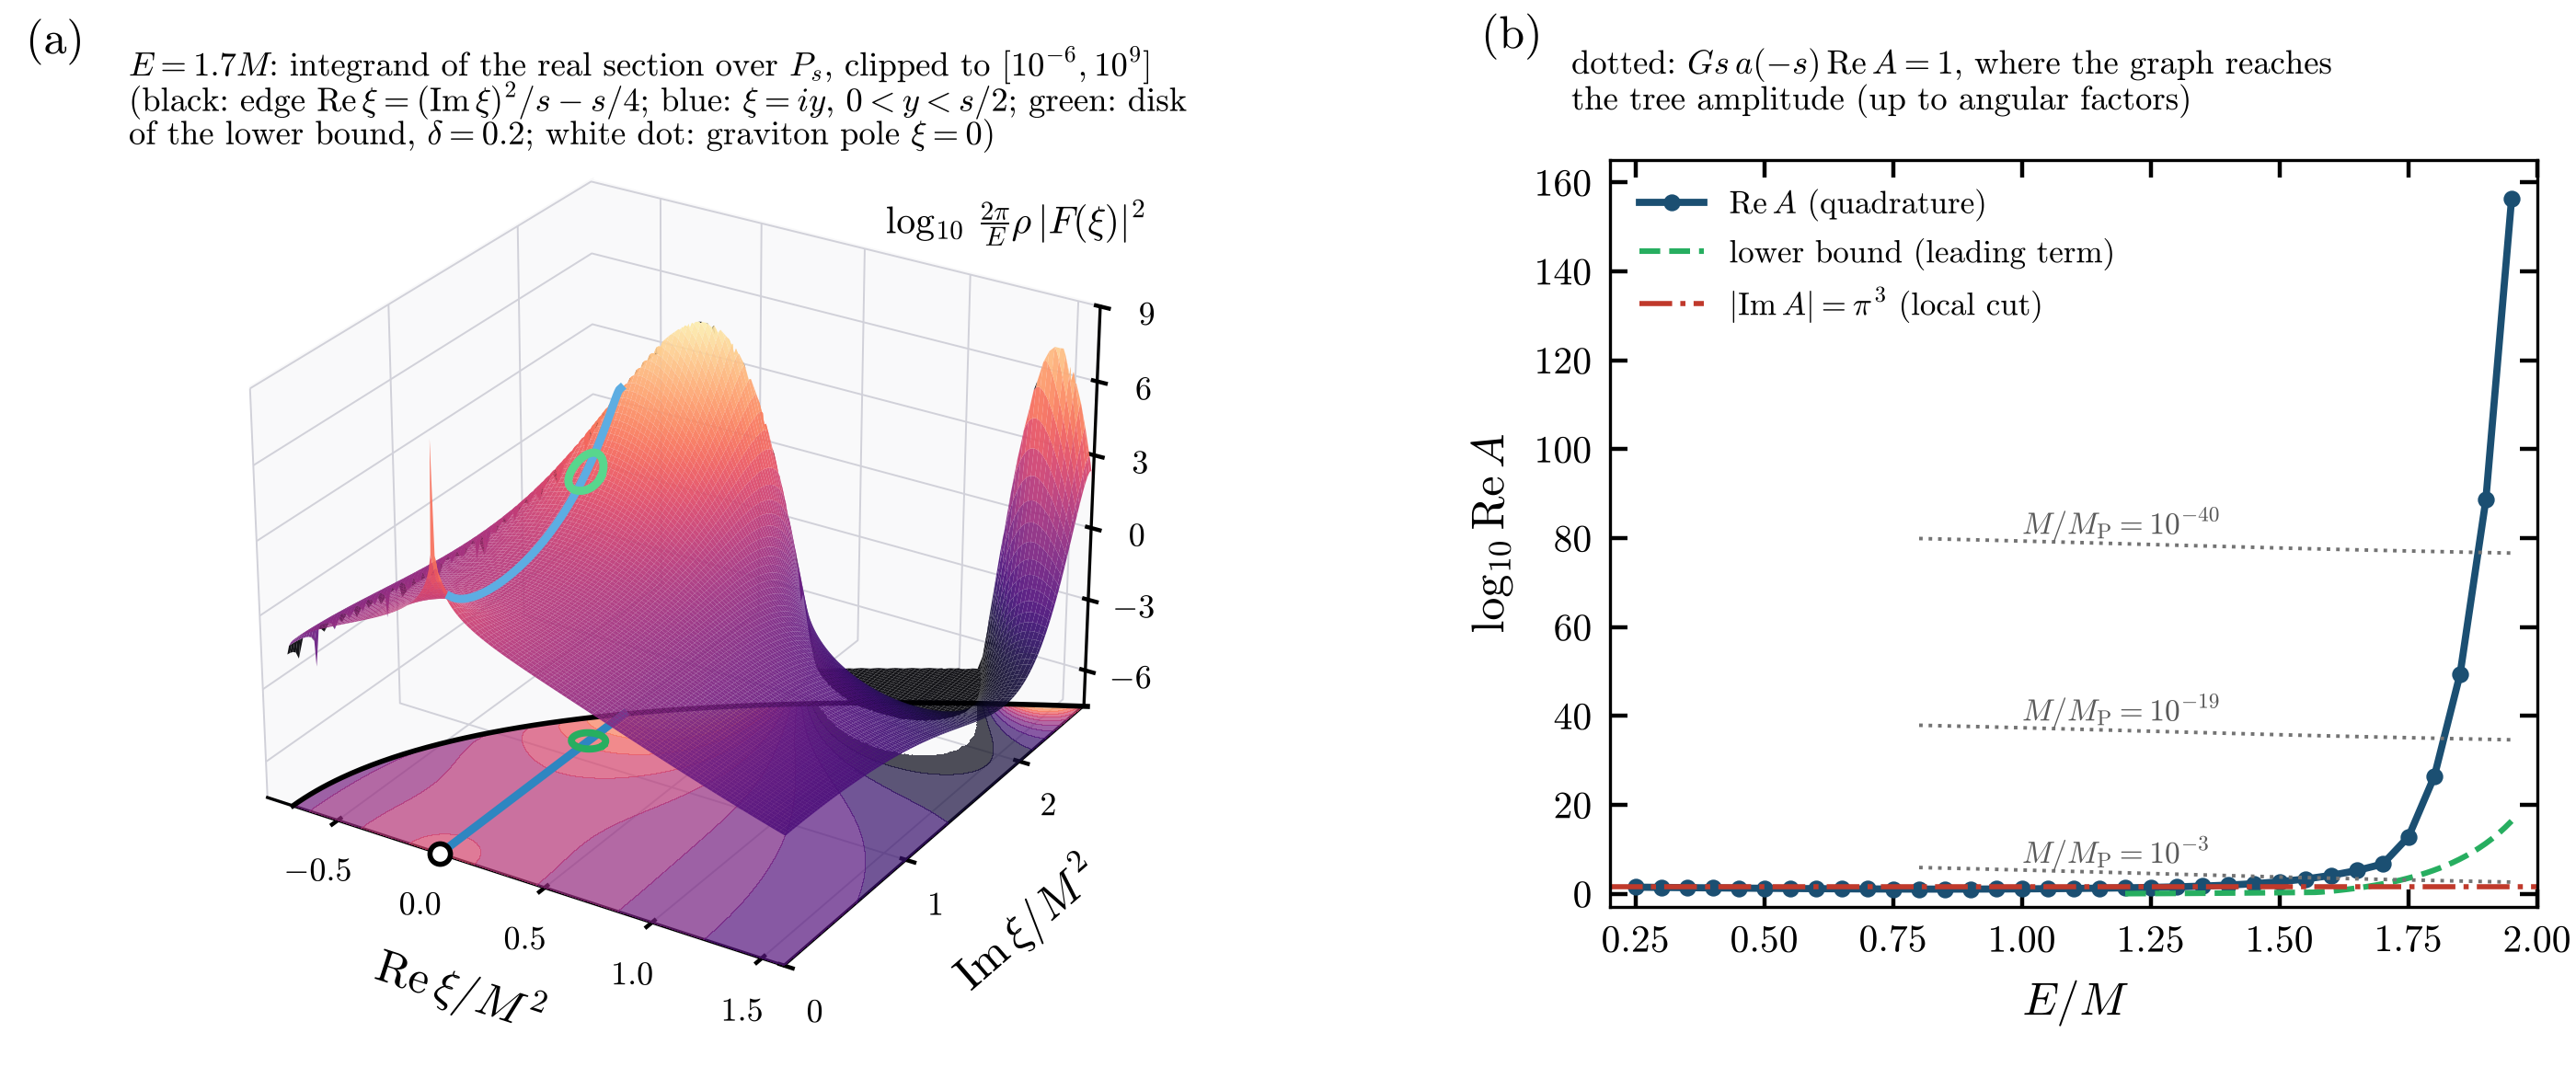
\includegraphics[width=\textwidth]{figs/fig_bubble.png}\\[2pt]
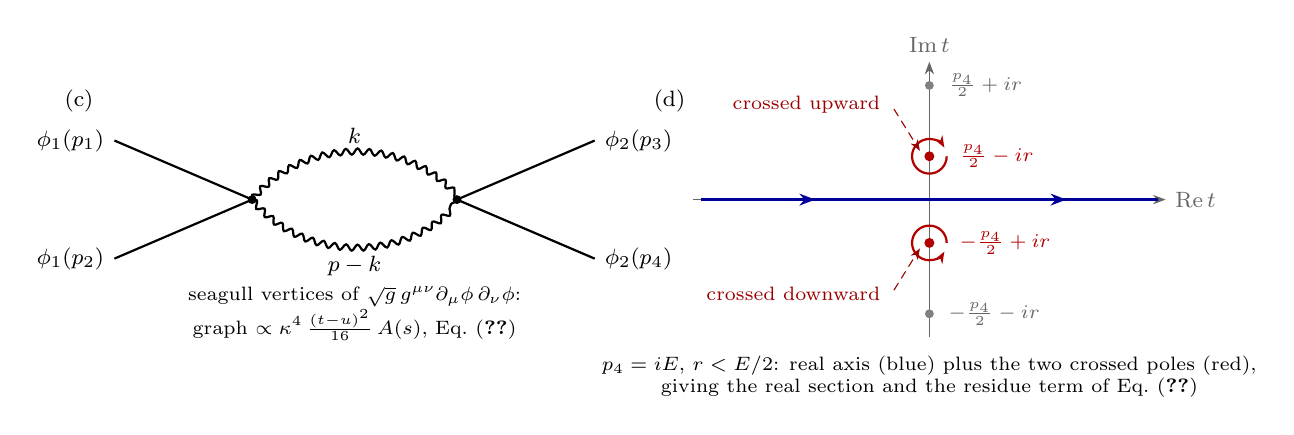
\begin{tikzpicture}[font=\footnotesize]
\begin{scope}[shift={(0,0)}]
\node at (-2.2,1.25) {(c)};
\draw[thick] (-1.75,0.75) -- (0,0) node[pos=0,left] {$\phi_1(p_1)$};
\draw[thick] (-1.75,-0.75) -- (0,0) node[pos=0,left] {$\phi_1(p_2)$};
\draw[grav] (0,0) to[bend left=50] node[above] {$k$} (2.6,0);
\draw[grav] (0,0) to[bend right=50] node[below] {$p-k$} (2.6,0);
\draw[thick] (2.6,0) -- (4.35,0.75) node[right] {$\phi_2(p_3)$};
\draw[thick] (2.6,0) -- (4.35,-0.75) node[right] {$\phi_2(p_4)$};
\fill (0,0) circle (1.6pt); \fill (2.6,0) circle (1.6pt);
\node[align=center,font=\scriptsize] at (1.3,-1.45) {seagull vertices of $\sqrt g\,g^{\mu\nu}\partial_\mu\phi\,\partial_\nu\phi$:\\ graph $\propto\kappa^4\,\tfrac{(t-u)^2}{16}\,A(s)$, Eq.~\eqref{eq:bubble}};
\end{scope}
\begin{scope}[shift={(8.6,0)}]
\node at (-3.3,1.25) {(d)};
\draw[-{Stealth[length=1.6mm]},black!60] (-3.0,0) -- (3.0,0) node[right] {$\mathrm{Re}\,t$};
\draw[-{Stealth[length=1.6mm]},black!60] (0,-1.75) -- (0,1.75) node[above] {$\mathrm{Im}\,t$};
\draw[very thick,blue!60!black,postaction={decorate},decoration={markings,mark=at position 0.25 with {\arrow{Stealth[length=2mm]}},mark=at position 0.8 with {\arrow{Stealth[length=2mm]}}}] (-2.9,0) -- (2.9,0);
\fill[red!70!black] (0,0.55) circle (1.8pt); \fill[red!70!black] (0,-0.55) circle (1.8pt);
\node[red!70!black,font=\scriptsize,anchor=west] at (0.26,0.55) {$\tfrac{p_4}2-ir$};
\node[red!70!black,font=\scriptsize,anchor=west] at (0.26,-0.55) {$-\tfrac{p_4}2+ir$};
\fill[black!50] (0,1.45) circle (1.6pt); \fill[black!50] (0,-1.45) circle (1.6pt);
\draw[red!70!black,thick,-{Stealth[length=1.5mm]}] (0.22,0.55) arc (0:-330:0.22);
\draw[red!70!black,thick,-{Stealth[length=1.5mm]}] (0.22,-0.55) arc (0:330:0.22);
\draw[red!60!black,densely dashed,-{Stealth[length=1.4mm]}] (-0.45,-1.15) -- (-0.12,-0.62);
\draw[red!60!black,densely dashed,-{Stealth[length=1.4mm]}] (-0.45,1.15) -- (-0.12,0.62);
\node[red!60!black,font=\scriptsize,align=left,anchor=east] at (-0.5,1.2) {crossed upward};
\node[red!60!black,font=\scriptsize,align=left,anchor=east] at (-0.5,-1.2) {crossed downward};
\node[black!60,font=\scriptsize,anchor=west] at (0.12,1.45) {$\tfrac{p_4}2+ir$};
\node[black!60,font=\scriptsize,anchor=west] at (0.12,-1.45) {$-\tfrac{p_4}2-ir$};
\node[font=\scriptsize,align=center] at (0,-2.25) {$p_4=iE$, $r<E/2$: real axis (blue) plus the two crossed poles (red),\\ giving the real section and the residue term of Eq.~\eqref{eq:bubbledec}};
\end{scope}
\end{tikzpicture}
\caption{The one-loop bubble in the Efimov--Pius--Sen prescription, for the skeleton with $n=4$. (a) The integrand of the real section of Eq.~\eqref{eq:bubbledec} at $E=1.7M$, $\log_{10}[(2\pi/E)\rho|F(\xi)|^2]$, over the region $P_s$ of the $\xi$ plane that the loop momentum covers, upper half (the lower half is its mirror image); the surface is clipped to $[10^{-6},10^{9}]$, and the flat dark patch is a trough where $|a|$ is large. Its edge, $\mathrm{Re}\,\xi=(\mathrm{Im}\,\xi)^2/s-s/4$, is the black curve on the floor, where $\rho=r=0$. The blue segment is $\xi=iy$, $0<y<s/2$, where $|F|^2=y^{-2}\exp[n\Ein^-(y^2/M^4)]$, and the green circle is the disk used in the bound~\eqref{eq:bubblebound} with $\delta=0.2$, both drawn on the floor and lifted onto the surface; the white dot is the graviton pole $\xi=0$, whose logarithmic singularity is removed by the subtraction. The ridges near the edge lie where $\mathrm{Re}\,\xi^2$ is most negative and the oscillating part of $\log a$, of size $\frac n2|E_1(\xi^2/M^4)|$, has the sign that makes $|a|$ small. (b) $\log_{10}\mathrm{Re}\,A$ against $E/M$ from Eq.~\eqref{eq:bubbledec} (dots), the leading term of the lower bound~\eqref{eq:bubblebound} maximized over $\delta$ (green, dashed), and $\log_{10}|\mathrm{Im}\,A|=\log_{10}\pi^3$ (red, dash-dotted). The dotted curves are $\log_{10}[(M_{\rm P}/M)^2/(s\,a(-s))]$ for $M/M_{\rm P}=10^{-3},10^{-19},10^{-40}$; where $\mathrm{Re}\,A$ crosses one of them, the graph reaches the tree amplitude, up to angular factors. (c) The graph: each pair of scalars annihilates into two gravitons through the seagull vertex, and the loop integral is $A$. (d) The contour in the plane of the loop energy $t$ at the physical point: of the four poles of the two propagators, two have crossed the real axis during the continuation, and the contour that keeps its ends fixed is the real axis plus circles around them.}
\label{fig:bubble}
\end{figure*}

\subsection{The size of amplitudes}
\label{sec:size}

Unitarity in this sense constrains the cuts of amplitudes, not their size. For actions quadratic in the Ricci tensor and the scalar curvature, with form factors inserted, the on-shell tree amplitudes coincide with those of general relativity for any number of gravitons~\cite{Dona2015}, and $R+G_{\mu\nu}F(\Box)R^{\mu\nu}$ is of that type. The quartic operators are different. Those built from $R$ and $R_{\mu\nu}$ add nothing to on-shell graviton scattering, because the linearized Ricci tensor of an on-shell graviton vanishes. The Riemann operator does add something: a contact term of order $G|s_3|E^{2n+2}/M^{2n}$ at center-of-mass energy $E$, which grows faster than any amplitude of general relativity and reaches order one at $E_*=(M^{2n}/G|s_3|)^{1/(2n+2)}$. That scale can be avoided. Set $s_3=0$ and solve for $s_1$ and $s_2$ alone, with the upper-left $2\times2$ block of Eq.~\eqref{eq:killcontrib}, whose determinant is $-12/c^2$. The Gauss--Bonnet pole then stays, but $\int\sqrt g\,E$ is topological in four dimensions and does not enter the $S$ matrix.

With $s_3=0$ every tree amplitude of gravitons is that of general relativity, and at fixed angle it grows like $GE^2$, reaching order one near the Planck energy $E_{\rm P}=G^{-1/2}$. The loops set a lower scale. The one-loop graph of Sec.~\ref{sec:bubble}, finite at every energy, overtakes the tree amplitude of its process between $1.4M$ and $1.9M$ for any $M$ between $10^{-40}M_{\rm P}$ and $10^{-2}M_{\rm P}$. The loop expansion, finite term by term, is therefore an expansion in a small number only up to energies of order $M$, and for $M\ll M_{\rm P}$ the theory becomes strongly coupled well below the Planck energy at which general relativity does. The form factor that removes the divergences also lowers the scale at which perturbation theory ends.

Matter that couples minimally to the metric behaves differently, because its gravitational scattering at tree level goes through the propagator~\eqref{eq:prop} itself. Between conserved sources the propagator gives $T_1\!\cdot T_2-\frac12T_1T_2$ divided by $p^2a(p^2)$, and for two distinct massless scalars $T_1\!\cdot T_2-\frac12T_1T_2=-su$ in terms of the Mandelstam variables. The one-graviton exchange is therefore the amplitude of general relativity divided by the form factor at the momentum transfer,
\begin{equation}
\label{eq:matter}
|A(s,t)|=\frac{8\pi G\,|su|}{|t|\,a(-t)} ,
\end{equation}
with $a$ evaluated at the Euclidean point $p^2=-t>0$. At a fixed scattering angle $\theta$ in the center-of-mass frame, $-t=s\sin^2(\theta/2)$ and $-u=s\cos^2(\theta/2)$, and the lower half of the two-sided bound~\eqref{eq:twosided-real} gives
\[
|A|\le8\pi GM^2\,C_\Pi\,\frac{\cos^2(\theta/2)}{\sin^4(\theta/2)}\,\frac{x}{(1+x^2)^{n/2}},\qquad x=\frac{-t}{M^2},
\]
with $C_\Pi=e^{-nm_\psi+\|R_\Pi\|}$. The last factor is at most $(n-1)^{(n-1)/2}/n^{n/2}$, which is $0.325$ for $n=4$, and it falls like $x^{1-n}$. At every fixed angle the tree amplitude for the gravitational scattering of matter therefore rises like $GE^2$ only up to $E\sim M$, then falls like $GM^2(M/E)^{2n-2}$, and never exceeds a number of order $GM^2=(M/M_{\rm P})^2$. For $M$ below the Planck mass, matter does not scatter strongly through one graviton at any energy. This is a tree-level statement. At one loop the same kind of process has the graph of Sec.~\ref{sec:bubble}, which overtakes the tree amplitude above an energy between $1.4M$ and $1.9M$, so the tree-level bound describes the theory only below that energy. The finiteness proof of Sec.~\ref{sec:finite} concerns pure gravity, and loops of matter fields are not treated here. The forward peak at $|t|\to0$ is the Newtonian one of general relativity, an infrared effect untouched by the form factor.

\subsection{In what sense the theory is ultraviolet complete}
\label{sec:complete}

A quantum field theory is ultraviolet complete in perturbation theory when its loop expansion is defined at every order without a cutoff and without new degrees of freedom: each term is finite with fixed bare couplings, the $S$ matrix is unitary order by order, and the asymptotic states are the same at every energy. For $n\ge4$, almost every realization of a gas obeying A1 and A2, and the assumption on asymptotic states that is made for general relativity, Secs.~\ref{sec:finite} and \ref{sec:unitarity} establish all three. The bare couplings do not depend on the regulator (Sec.~\ref{sec:nocutoff}), the physical $S$ matrix is unitary at every loop order, and its only asymptotic states are the two helicities of the graviton. No physical coupling is renormalized, so none of them runs. The perturbative renormalization group of the physical couplings is trivial, there is no Landau pole, and no order of perturbation theory calls for a new coupling, whereas in general relativity the two-loop divergence does~\cite{GoroffSagnotti1986}. In this sense, and to every order in $\kappa$, the theory of the gas is ultraviolet complete.

Finite and unitary at every order is not the same as small at every energy. Section~\ref{sec:bubble} shows that individual terms of the loop expansion become large above an energy between $1.4M$ and $1.9M$, so the expansion is useful only below that scale, as the loop expansion of general relativity is useful only below $E_{\rm P}$. Ultraviolet complete in perturbation theory means here that the loop expansion is defined and finite at every order and at every energy, not that it converges, or that its terms are small, above $M$. One step beyond it can be taken rigorously, at the level of the free field. The spin-two part of the quadratic action~\eqref{eq:S2}, $\frac12p^2a(p^2)\,h\Pt h$, is positive on the Euclidean axis, so it defines a Gaussian probability measure, in infinite volume, on the gauge-invariant field $\Pt h$, with covariance $\Pt/(p^2a)$; the covariance is integrable at small $p$ in four dimensions, so there is no infrared obstruction either. For each Fourier mode the linearized Weyl tensor obeys $C\cdot C=\frac{p^4}2\,h\Pt h$, and $\operatorname{tr}\Pt=5$, so the Weyl tensor of $\kappa h$ has
\begin{multline}
\label{eq:weyl}
\bE\,C_{\mu\nu\rho\sigma}C^{\mu\nu\rho\sigma}(x)=\frac{5\kappa^2}2\int\frac{\dd^4p}{(2\pi)^4}\,\frac{p^2}{a(p^2)}\\
=\frac{5GM^6}{\pi}\int_0^\infty\frac{x^2\,\dd x}{a(x)} .
\end{multline}
By the two-sided bound~\eqref{eq:twosided-real} the integral converges exactly when $n\ge4$, and at $n=3$ it diverges logarithmically, the same threshold as in the power counting of Sec.~\ref{sec:degree}. For the skeleton with $n=4$ the integral lies between $\pi/(4\hat c)$ and $\pi/4$ and equals $0.4237$, so the root-mean-square Weyl curvature at a point is $0.82\,M^3/M_{\rm P}$, small compared with $M^2$ whenever $M\ll M_{\rm P}$. The same estimate applied to $C(x)-C(0)$, with $1-\cos y\le2|y/2|^{2\alpha}$, gives $\bE|C(x)-C(0)|^2\le C_\alpha|Mx|^{2\alpha}$ for every $\alpha<\min(1,n-3)$. The field is Gaussian, so Kolmogorov's continuity criterion applies, and the curvature of almost every free configuration is a H\"older-continuous function. In general relativity the integral in Eq.~\eqref{eq:weyl} grows like the sixth power of a cutoff, the free field is a distribution, and every product of fields at a point has to be renormalized. Here no product of curvatures at a point needs renormalization: the free graviton of the gas has no short-distance singularity at all. This Gaussian measure is a Euclidean random field, and it is not reflection positive, so the Osterwalder--Schrader reconstruction~\cite{OsterwalderSchrader1973,GlimmJaffe1987} does not turn it into a quantum field with a positive Hilbert space. Reflection positivity of a free field requires its covariance to be a Stieltjes function, $\int\dd\varrho(m^2)/(z+m^2)$ with a positive measure, and a Stieltjes function that is analytic across the negative real axis is $c/z$, since $\varrho$ is the jump across that axis; $1/(za)$ is analytic there except at $z=0$ and is not $c/z$.\footnote{The same holds for the covariance $\Pt/(p^2a)$ of the spin-two field, whose components are $1/a(p^2)$ times rational functions of the momentum; the obstruction is the factor $1/a$, which is entire and not constant.} The Hilbert space of the theory is the Fock space of the asymptotic gravitons of Sec.~\ref{sec:quartets}, as in string field theory, and the statement about the curvature is a statement about the Euclidean field.

What is missing for a complete construction is the interacting measure, defined by a Euclidean functional integral or by a proof that the perturbation series is Borel summable. That would make the theory ultraviolet complete without qualification. We do not have it, and two obstacles are concrete. The quadratic action~\eqref{eq:S2} is that of general relativity multiplied by $a(p^2)$, so its spin-zero part, with coefficient $-2$, is unbounded below exactly as the conformal factor of general relativity is~\cite{GibbonsHawkingPerry1978}. Rotating that mode to imaginary values, as Gibbons, Hawking and Perry do, makes the quadratic action positive here too, but the rotation is a prescription, and the gas does not remove the need for it. The resummed propagator $1/(za+\Sigma)$ may also acquire complex poles from the self-energy~\cite{Shapiro2015}, which no finite order sees. At one loop they do not appear where perturbation theory is controlled. On the region $\Omega$ of Sec.~\ref{sec:cutkosky} the one-loop self-energy obeys the estimate $|\Sigma(z)|\le C\kappa^2M^2|z\,a(z)|$ for $|z|\ge M^2$, which follows from the vertex bound,\footnote{In the self-energy the external momentum $p$ enters both vertices. Where the loop momentum $k$ is at most of order $|p|$, each cubic vertex is bounded by $C\kappa M^2(|p|/M)^{2n+2}$ by Eq.~\eqref{eq:vertexbound} with the coupling restored, one propagator by $C(M/|p|)^{2n+2}M^{-2}$, and the other is integrated, $\int\dd^4k\,|k^2a(k^2)|^{-1}$ over $|k|\lesssim|p|$ being at most $CM^2$ for $n\ge2$; together $|\Sigma|\le C\kappa^2M^4(|p|/M)^{2n+2}$, which is $C\kappa^2M^2|za|$ by the cone asymptotics~\eqref{eq:cone-real}. Where $|k|\gg|p|$ the integrand has degree $4$, and after the subtraction of Sec.~\ref{sec:cutkosky} the remainder grows at most like $|p|^4\log|p|$, which is smaller. On $\Omega$ the same bounds hold with $|p|$ replaced by $|\mathrm{Re}\,p|$ plus a constant, as in (P3). At small $|z|$ the self-energy is that of general relativity, of order $\kappa^2|z|^2\log|z|$.} and $|z\,a(z)|\ge c'|z|$ on the compact part of $\Omega$. For $M\ll M_{\rm P}$ the propagator resummed with the one-loop self-energy therefore has no pole in $\Omega$ other than $z=0$. Complex poles can lie only in the wedges around the imaginary axis where $|a|$ is small, the region that makes the bubble of Sec.~\ref{sec:bubble} large, and they belong to the strongly coupled regime above $M$. Neither obstacle is special to the gas. Both are open for every nonlocal theory of this class, and no nontrivial relativistic quantum field theory in four dimensions is yet known to satisfy the Wightman axioms~\cite{JaffeWitten2006}. Classically, the linearized field of any mass below $m_c\sim M_{\rm P}^2/M$ is weak everywhere and has no horizon (Sec.~\ref{sec:classical}). Collisions at higher energies, where general relativity forms black holes, are a nonlinear problem that this paper leaves open.

\begin{table*}[t]
\caption{Bookkeeping of divergences. ``Removed'' means that the corresponding pole or singularity is absent for $n\ge4$ with the tuning~\eqref{eq:tuning}; the third column gives the reason.}
\label{tab:divergences}
\begin{ruledtabular}
\begin{tabular}{L{4.6cm}L{2.5cm}L{9.6cm}}
divergence & fate & reason\\
\colrule
one loop, $\int\sqrt g$ and $\int\sqrt g\,R$ (running of $\Lambda$, $G$) & absent for $n\ge4$ & one-loop poles are those of a local theory with no dimensionful coupling; saturation (S3) and fine graining (G), Sec.~\ref{sec:form}; the finite vacuum energy has mean $3nM^4/(64\pi^2)$, Sec.~\ref{sec:vacuum}\\
one loop, $R^2$, $R_{\mu\nu}R^{\mu\nu}$, $E$ & removed & three quartic operators, triangular matrix with determinant $-24/c^3$, Eqs.~\eqref{eq:killcontrib}, \eqref{eq:tuning}\\
two or more loops, overall & absent for $n\ge4$ & vertex bound and Weinberg's theorem, Sec.~\ref{sec:degree}\\
one-loop subgraphs, gauge-invariant part & removed & equals the one-loop pole of the full metric, which vanishes after tuning\\
one-loop subgraphs, BRST-exact part & present off shell & renormalizes the gauge-fixing sector; no effect on the $S$ matrix, Sec.~\ref{sec:finite}\\
power-law terms ($\Lambda^4$, $\Lambda^2$ with a cutoff) & scheme artifacts & absent in any analytic regularization; the finite part does not depend on the regulator, Sec.~\ref{sec:nocutoff}\\
soft gravitons on shell (infrared) & physical & as in general relativity; cancel in inclusive rates~\cite{Weinberg1965}\\
static potential at $r\to0$ (classical) & removed & $\Phi_N(0)$ finite; Gamma-function bounds for the skeleton, Sec.~\ref{sec:classical}\\
extra poles of the propagator & absent & almost every realization entire and zero-free, by (S5); resonant branes would give complex pairs, Eq.~\eqref{eq:qzeros}\\
\end{tabular}
\end{ruledtabular}
\end{table*}


\section{Newtonian limit}
\label{sec:classical}

The quartic operators do not touch the propagator, so the static field of a point mass follows from Eq.~\eqref{eq:prop} alone. For a source $T_{\mu\nu}=m\,\delta^3(\mathbf x)\,u_\mu u_\nu$ at rest, the linearized field is the one of general relativity with $1/\mathbf k^2$ replaced by $1/(\mathbf k^2a(\mathbf k^2))$, because the form factor multiplies both projectors by the same scalar. In general relativity the computation gives $\tilde\Phi_N(\mathbf k)=-4\pi Gm/\mathbf k^2$, so here
\begin{equation}
\label{eq:PhiK}
\tilde\Phi_N(\mathbf k)=-\frac{4\pi Gm}{\mathbf k^2\,a(\mathbf k^2)} ,
\end{equation}
and the Fourier transform of a radial function in three dimensions,
\[
\int\frac{\dd^3k}{(2\pi)^3}\,e^{i\mathbf k\cdot\mathbf x}f(k)=\frac1{2\pi^2r}\int_0^\infty k\sin(kr)f(k)\,\dd k ,
\]
gives
\begin{equation}
\label{eq:pot}
\Phi_N(r)=-\frac{2Gm}{\pi r}\int_0^\infty\frac{\sin kr}{k\,a(k^2)}\,\dd k .
\end{equation}
With $a=1$ the integral is $\pi/2$ and Eq.~\eqref{eq:pot} is Newton's potential. With the form factor of the gas, the integrand is bounded by $1/a(k^2)$ uniformly in $r$, and $1/a$ falls like $k^{-2n}$. Below we find how deep the well is, how fast the potential approaches $-Gm/r$, and how large a mass the linearized description can carry; all three have closed answers.

\subsection{Depth of the well}

At the origin $\sin(kr)/(kr)\to1$, and
\begin{equation}
\label{eq:pot0}
\Phi_N(0)=-\frac{2Gm}{\pi}\,I_n,\qquad I_n=\int_0^\infty\frac{\dd k}{a(k^2)} .
\end{equation}
Since $|\sin(kr)/(kr)|\le1$ and the integrand of $I_n$ is positive, $|\Phi_N(r)|\le|\Phi_N(0)|$ for every $r$: the potential is deepest at the center, and it is finite there. The value of $I_n$ is bracketed from both sides by elementary integrals, and the bracket is narrow. We give the numbers for the skeleton, $a=\hat a$. A realization has $a=\hat a\,e^{R_\Pi}$ with $R_\Pi$ bounded on the real axis, so its $I_n$ lies between $e^{-\sup R_\Pi}$ and $e^{-\inf R_\Pi}$ times the skeleton value, the supremum and infimum being taken over the real axis; the qualitative statements below, a finite well, $2n-2$ continuous derivatives and an approach to Newton's law faster than any power, hold for almost every realization as they stand, because they use only Eq.~\eqref{eq:twosided-real}, the derivative bounds that follow Eq.~\eqref{eq:cone-real}, which take the place of Eq.~\eqref{eq:aderiv}, and $a-1=O(k^4)$; only the constants change from one realization to another.

For an upper bound we use the left inequality of Eq.~\eqref{eq:twosided}, $a\ge(1+k^4/M^4)^{n/2}$. With $t=k^4/M^4$,
\begin{equation}
\label{eq:Jn}
I_n\le\int_0^\infty\frac{\dd k}{(1+k^4/M^4)^{n/2}}=\frac M4\int_0^\infty\frac{t^{-3/4}\,\dd t}{(1+t)^{n/2}}=J_n,
\end{equation}
where
\begin{equation}
\label{eq:Jn-closed}
J_n=\frac M4\,B\Bigl(\frac14,\frac n2-\frac14\Bigr)=\frac M4\,\frac{\Gamma(\frac14)\Gamma(\frac n2-\frac14)}{\Gamma(\frac n2)} .
\end{equation}
For even $n=2m$ the gamma functions collapse. From $\Gamma(m-\frac14)=\Gamma(\frac34)\prod_{j=1}^{m-1}(j-\frac14)$ and the reflection formula $\Gamma(\frac14)\Gamma(\frac34)=\pi\sqrt2$,
\begin{equation}
\label{eq:Jeven}
J_{2m}=\frac{\pi\sqrt2}{4}\,M\prod_{j=1}^{m-1}\Bigl(1-\frac1{4j}\Bigr),
\end{equation}
so $J_4=\frac{3\pi\sqrt2}{16}M$, $J_6=\frac{21\pi\sqrt2}{128}M$, $J_8=\frac{77\pi\sqrt2}{512}M$, and so on.

For a lower bound the right inequality of Eq.~\eqref{eq:twosided} is too weak, since $\hat c=e^{n\gE/2}$ grows exponentially with $n$. A better one comes from the definition of $\Ein$ itself. The integrand $(1-e^{-t})/t$ is at most $1$, so $\Ein(w)\le w$ for $w\ge0$, and therefore $a(k^2)\le\exp(\frac n2k^4/M^4)$. Then
\begin{equation}
\label{eq:Kn}
I_n\ge\int_0^\infty e^{-nk^4/(2M^4)}\,\dd k=\frac M4\,\Gamma\Bigl(\frac14\Bigr)\Bigl(\frac2n\Bigr)^{1/4}\equiv K_n .
\end{equation}
The two bounds are close. Their ratio is $J_n/K_n=(n/2)^{1/4}\,\Gamma(\frac n2-\frac14)/\Gamma(\frac n2)$, and Wendel's inequality for ratios of gamma functions~\cite{Wendel1948},\footnote{For $x>0$ and $0<s<1$, H\"older's inequality with exponents $1/s$ and $1/(1-s)$ applied to $\Gamma(x+s)=\int_0^\infty t^{s\cdot x}\,t^{(1-s)(x-1)}e^{-t}\,\dd t$ gives $\Gamma(x+s)\le\Gamma(x+1)^s\Gamma(x)^{1-s}=x^s\Gamma(x)$. The same inequality with $x\to x+s$ and $s\to1-s$ gives $\Gamma(x+1)\le(x+s)^{1-s}\Gamma(x+s)$, that is $\Gamma(x+s)\ge x\,\Gamma(x)/(x+s)^{1-s}$. Together, $(x/(x+s))^{1-s}\le\Gamma(x+s)/(x^s\Gamma(x))\le1$. We use the lower half with $x=\frac n2-\frac14$ and $s=\frac14$.} $\Gamma(x+s)\ge x\,\Gamma(x)\,(x+s)^{s-1}$ with $x=\frac n2-\frac14$, $s=\frac14$, gives $J_n/K_n\le 2n/(2n-1)$. Hence
\begin{equation}
\label{eq:pot0-sharp}
\begin{gathered}
\Phi_N(0)=-\frac{\Gamma(\frac14)}{2\pi}\Bigl(\frac2n\Bigr)^{1/4}GmM\Bigl[1+\frac{\theta_n}{2n-1}\Bigr],\\
0\le\theta_n\le1 .
\end{gathered}
\end{equation}
For $n=4$, Eqs.~\eqref{eq:Jn} and \eqref{eq:Kn} give $0.4852\le|\Phi_N(0)|/(GmM)\le0.5303$, and the value of the integral itself, obtained by quadrature as a check, is $0.5100$; for $n=6$ the bracket is $[0.4385,0.4640]$ around $0.4519$. For comparison, the Gaussian form factor $e^{p^2/M^2}$ gives $\Phi_N=-Gm\,\mathrm{erf}(Mr/2)/r$ and $|\Phi_N(0)|=GmM/\sqrt\pi\approx0.564\,GmM$~\cite{BGKM2012,EdholmKoshelevMazumdar2016}. The well of the gas is about ten percent shallower for $n=4$, and it becomes slowly shallower as the gas becomes denser, as $n^{-1/4}$.

The smoothness of $\Phi_N$ is fixed by the decay of Eq.~\eqref{eq:PhiK}. Since $\tilde\Phi_N=O(k^{-2n-2})$, the integral $\int\dd^3k\,|\mathbf k|^j|\tilde\Phi_N|$ converges for $j<2n-1$, and $\Phi_N$ has $2n-2$ continuous derivatives everywhere, the origin included. Equivalently, $\nabla^2\Phi_N=4\pi G\rho_{\rm eff}$ with an effective source
\begin{equation}
\label{eq:rhoeff}
\rho_{\rm eff}(\mathbf x)=m\int\frac{\dd^3k}{(2\pi)^3}\,\frac{e^{i\mathbf k\cdot\mathbf x}}{a(\mathbf k^2)},\qquad\int\rho_{\rm eff}\,\dd^3x=m,
\end{equation}
the total being $m$ because $a(0)=1$. The point mass is spread over a region of size $1/M$. The same two estimates of $a$ give
\[
\frac{\Gamma(\frac34)}{8\pi^2}\Bigl(\frac2n\Bigr)^{3/4}\le\frac{\rho_{\rm eff}(0)}{mM^3}\le\frac{1}{8\pi^2}\,B\Bigl(\frac34,\frac n2-\frac34\Bigr),
\]
and the linearized tidal tensor at the center, $\partial_i\partial_j\Phi_N(0)=\frac{4\pi G}3\rho_{\rm eff}(0)\,\delta_{ij}$, is finite. The curvature singularity of the linearized Schwarzschild field is gone.

\subsection{Approach to Newton's law}

Using $\int_0^\infty\sin(kr)\,\dd k/k=\pi/2$, write
\begin{equation}
\label{eq:delta}
\begin{gathered}
\Phi_N(r)=-\frac{Gm}r\bigl[1-\delta(r)\bigr],\\
\delta(r)=\frac2\pi\int_0^\infty\sin(kr)\,\chi(k)\,\dd k ,
\end{gathered}
\end{equation}
with $\chi(k)=[1-1/a(k^2)]/k$. Because $a(k^2)$ is an even entire function of $k$ and $1-1/a=O(k^4)$ (for the skeleton $\frac n2k^4/M^4+O(k^8)$ by Eq.~\eqref{eq:IR}), $\chi$ is odd, smooth, and $O(k^3)$ at the origin. At large $k$, Eq.~\eqref{eq:aderiv} and the chain rule give $\partial_k^j[1/a(k^2)]=O(k^{-2n-j})$, hence $\chi^{(j)}(k)=O(k^{-1-j})$. Now integrate by parts twice:
\[
\int_0^\infty\sin(kr)\,\chi(k)\,\dd k=-\frac1{r^2}\int_0^\infty\sin(kr)\,\chi''(k)\,\dd k .
\]
The boundary terms at infinity vanish because $\chi$ and $\chi'$ do, and those at $k=0$ vanish because $\chi(0)=0$ and $\sin0=0$. The function $\chi''$ is again odd and smooth, so the step can be repeated, and after $N$ repetitions
\begin{equation}
\label{eq:tail}
|\delta(r)|\le\frac2\pi\,\frac{\|\chi^{(2N)}\|_{L^1}}{r^{2N}}=\frac{C_N}{(Mr)^{2N}},
\end{equation}
where $C_N$ depends on $n$ and $N$ only, since $\chi(k)=M^{-1}\hat\chi(k/M)$ with $\hat\chi$ independent of $M$; for a realization $C_N$ depends also on the sizes $sM^2$ of its branes. As $N$ is arbitrary, the correction to Newton's law falls faster than any power of $1/(Mr)$. Figure~\ref{fig:newton} shows the potential for $n=4$ and the deviation for $n=4,\dots,8$; the oscillations of $\delta(r)$ come from the oscillating Fourier kernel and do not affect the bound.

This is the classical counterpart of the infrared statement of Sec.~\ref{sec:finite}. Every term of the low-momentum expansion of $1/a$ is a polynomial in $k^4$, and its Fourier transform is a contact term supported at $r=0$, so no inverse power of $r$ can appear at any order. The long-range quantum corrections of the effective field theory of gravity, which come from loops of massless particles and are non-analytic in $k$~\cite{Donoghue1994}, are not affected, because the infrared of the theory is that of general relativity. The inverse-square law has been tested down to $52\,\mu$m~\cite{Lee2020}, and by Eq.~\eqref{eq:tail} these tests require only $M\cdot52\,\mu\mathrm m\gg1$, that is $M$ well above $4\times10^{-3}$\,eV.

\begin{figure*}[t]
\centering
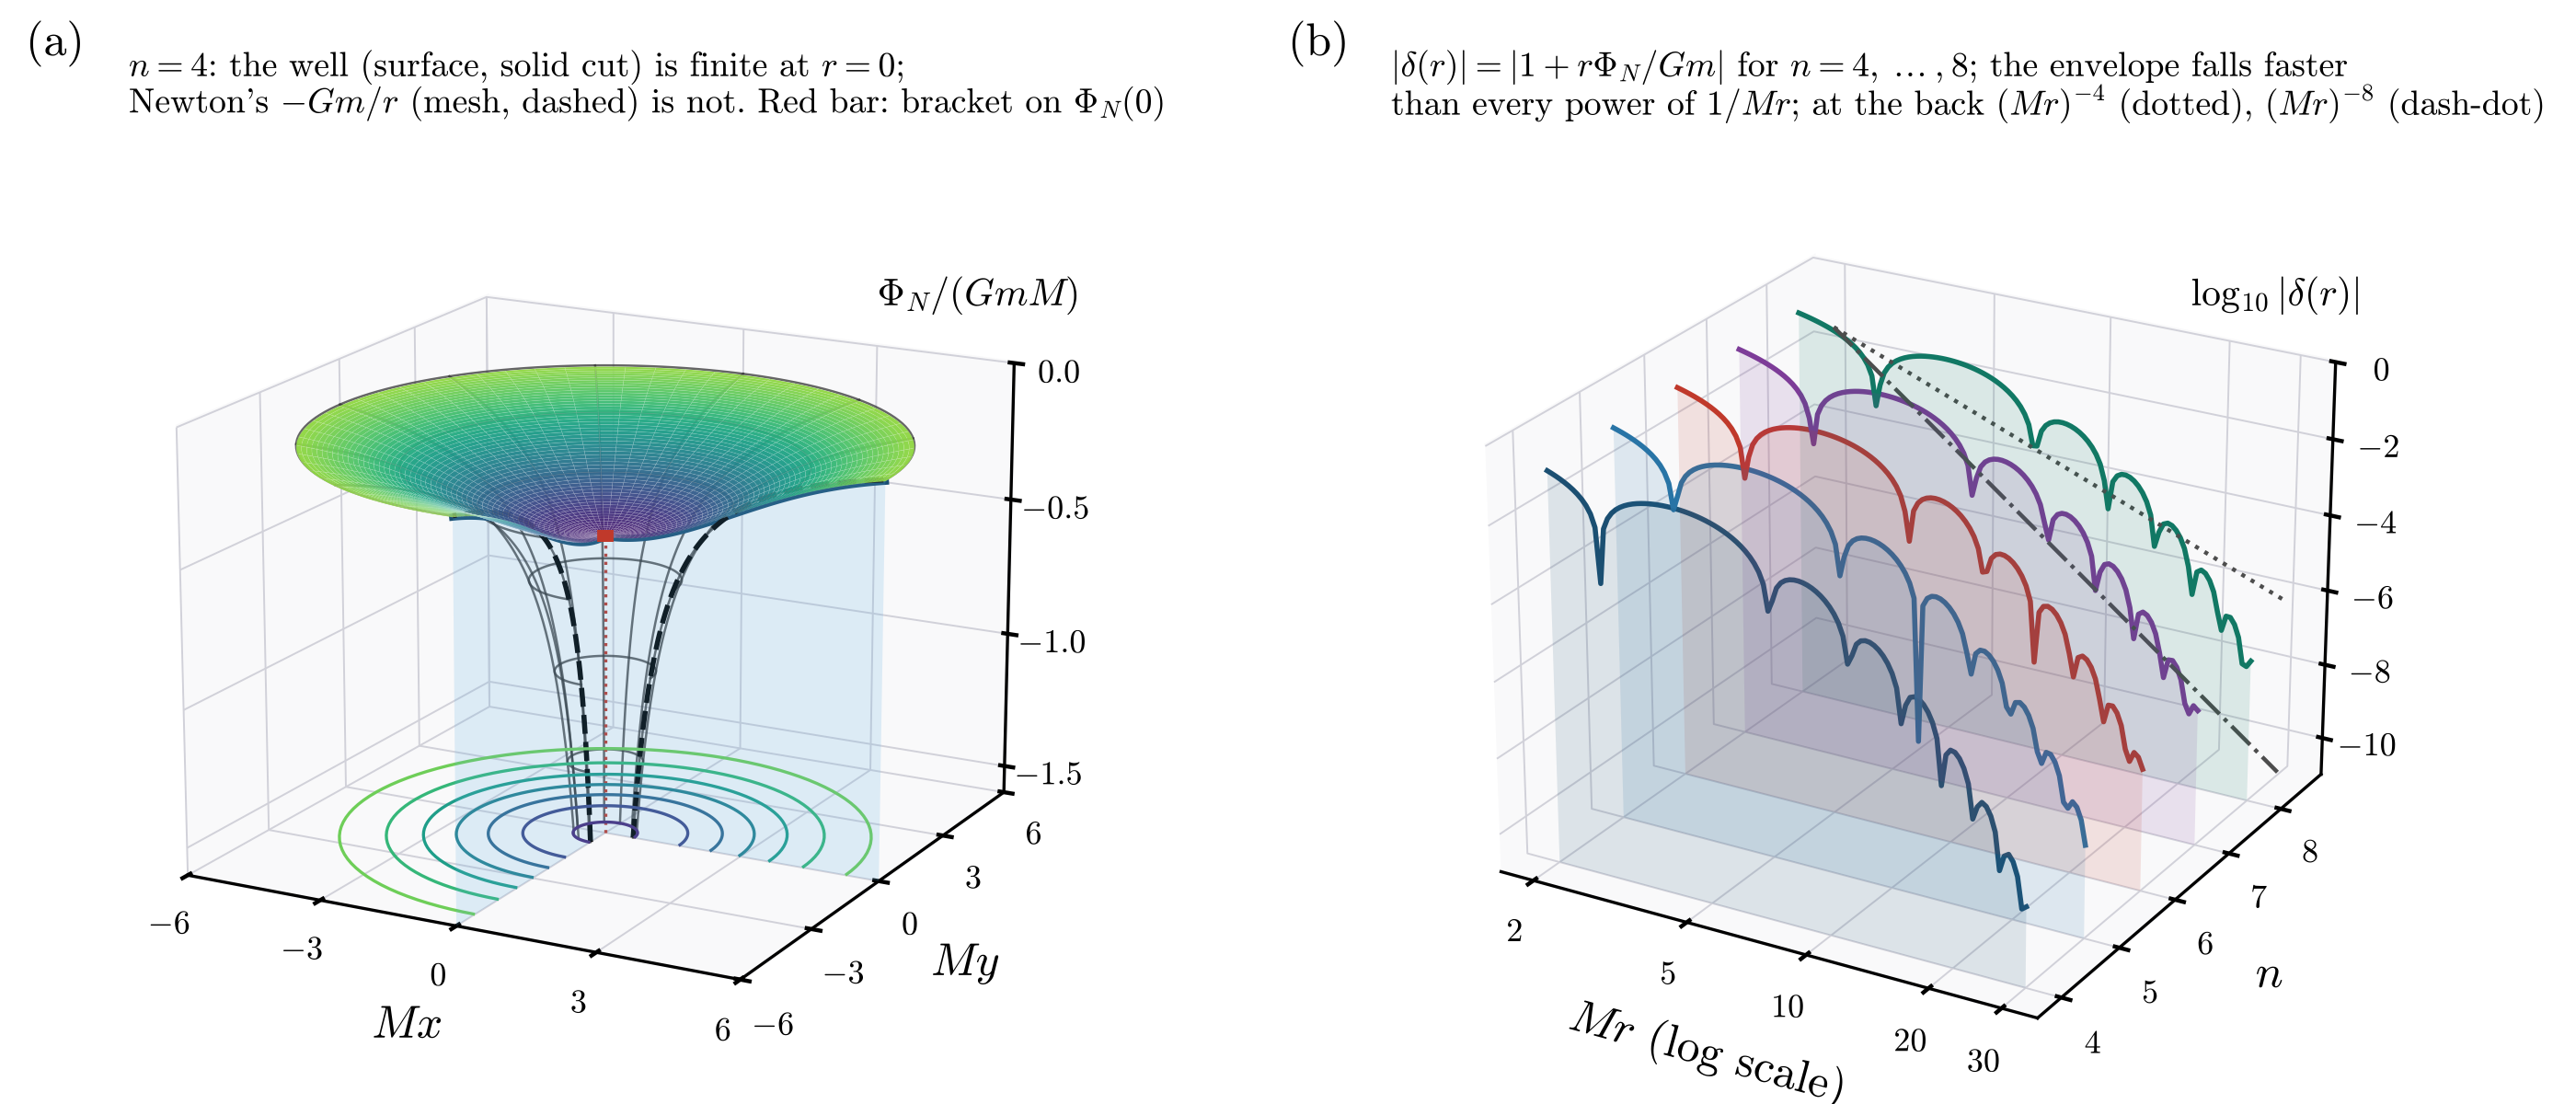
\includegraphics[width=\textwidth]{figs/fig_newton.png}
\caption{Newtonian limit. (a) The potential~\eqref{eq:pot} of a point mass for the skeleton with $n=4$, in units of $GmM$, drawn over a plane through the source with one quarter cut away. The surface and the solid profiles on the cut faces are $\Phi_N$; the mesh and the dashed profiles are Newton's $-Gm/r$. The red bar on the axis is the bracket $0.4852\le|\Phi_N(0)|/GmM\le0.5303$ of Eqs.~\eqref{eq:Jn} and \eqref{eq:Kn}; the floor carries the contours of $\Phi_N$. (b) The relative deviation $|\delta(r)|$ of Eq.~\eqref{eq:delta} for $n=4,\dots,8$, on logarithmic axes. The dips are zeros of $\delta$, which oscillates because of the Fourier kernel. The envelope falls faster than the reference lines $(Mr)^{-4}$ (dotted) and $(Mr)^{-8}$ (dash-dot) drawn at the back, as Eq.~\eqref{eq:tail} requires. The curves are numerical evaluations of the closed-form integrals and serve as illustration only.}
\label{fig:newton}
\end{figure*}

\subsection{Mass scale of the linear regime}

The linearized description is self-consistent at every point when $2|\Phi_N|<1$ everywhere, which by Eq.~\eqref{eq:pot0} and $|\Phi_N(r)|\le|\Phi_N(0)|$ happens exactly when
\begin{equation}
\label{eq:mc}
m<m_c=\frac{\pi}{4G\,I_n},\qquad\frac{\pi}{4GJ_n}\le m_c\le\frac{\pi}{4GK_n} .
\end{equation}
In units with $\hbar=c=1$ and $G=M_{\rm P}^{-2}$, $m_c=\mu_n\,M_{\rm P}^2/M$ with $\mu_n$ of order one; Table~\ref{tab:newton} gives it for several $n$. Below $m_c$ the weak-field expansion holds down to $r=0$ and the linearized field has no horizon. Above it, the expansion fails near the center and the question becomes nonlinear, which is beyond this paper. For $M$ near the Planck mass, $m_c$ is itself of order the Planck mass, so this is a statement about the smallest objects, not about astrophysical black holes.

\begin{table}[t]
\caption{Constants of the Newtonian limit, in units $M=1$ (for $J_n$, $K_n$, $I_n$) and $M_{\rm P}^2/M$ (for $m_c$). $K_n$ and $J_n$ are the closed-form bounds~\eqref{eq:Kn} and \eqref{eq:Jn-closed}; the column $I_n$ is a quadrature of Eq.~\eqref{eq:pot0}, given as a check. The bracket for $m_c$ is Eq.~\eqref{eq:mc}, and $\hat c=e^{n\gE/2}$. All entries are for the skeleton $\hat a$.}
\label{tab:newton}
\begin{ruledtabular}
\setlength{\tabcolsep}{3.2pt}
\begin{tabular}{ccccccc}
$n$ & $\hat c$ & $K_n$ & $I_n$ & $J_n$ & $\frac{|\Phi_N(0)|}{GmM}$ & $m_c$\\
\colrule
4 & 3.172 & 0.7622 & 0.8011 & 0.8330 & 0.5100 & $[0.943,1.030]$\\
5 & 4.234 & 0.7208 & 0.7485 & 0.7725 & 0.4765 & $[1.017,1.090]$\\
6 & 5.650 & 0.6887 & 0.7099 & 0.7289 & 0.4519 & $[1.077,1.140]$\\
7 & 7.540 & 0.6627 & 0.6797 & 0.6953 & 0.4327 & $[1.130,1.185]$\\
8 & 10.06 & 0.6409 & 0.6550 & 0.6682 & 0.4170 & $[1.175,1.225]$\\
10 & 17.92 & 0.6061 & 0.6165 & 0.6264 & 0.3925 & $[1.254,1.296]$\\
\end{tabular}
\end{ruledtabular}
\end{table}

\section{Discussion}
\label{sec:discussion}

Table~\ref{tab:compare} sets the result beside the better-known alternatives, for the quantities that decide the ultraviolet behavior: the form factor, the loop orders at which divergences occur, and the extra poles of the propagator. The last column records where the form factor comes from, which is the point of this paper.

\begin{table*}[t]
\caption{Ultraviolet behavior and pole content of the graviton propagator $1/(p^2a)$ in four dimensions. For a polynomial form factor of degree $N$ the residues of the extra poles add up to $-1$, so at least one is a ghost~\cite{Shapiro2015}. ${}^a$Renormalizable, with divergences at every order. ${}^b$Vertices grow exponentially and power counting is not available; see Ref.~\cite{Talaganis2015}. ${}^c$After adding operators cubic or quartic in curvature~\cite{ModestoRachwal2014}. ${}^d$For almost every realization of a gas obeying (G), with the one-loop tuning~\eqref{eq:tuning}; no coupling is renormalized at any order, and the physical $S$ matrix is unitary at every loop order in the Euclidean prescription (Sec.~\ref{sec:unitarity}); the loop expansion is useful only up to energies of order $M$ (Sec.~\ref{sec:bubble}).}
\label{tab:compare}
\begin{ruledtabular}
\begin{tabular}{L{3.9cm}L{3.6cm}L{3.6cm}L{2.4cm}L{3.2cm}}
theory & form factor $a(p^2)$ & divergent loop orders & extra poles & origin of $a$\\
\colrule
Einstein~\cite{tHooftVeltman1974,GoroffSagnotti1986} & $1$ & $L\ge1$ off shell, $L\ge2$ on shell & none & ---\\
Stelle~\cite{Stelle1977} & $1+p^2/M^2$ & all$^{\,a}$ & one massive ghost & local action\\
local, degree $N\ge2$~\cite{AsoreyLopezShapiro1997} & polynomial & $L\le(N+1)/(N-1)$ & $N$ & local action\\
Gaussian~\cite{BiswasMazumdarSiegel2006,BGKM2012} & $e^{p^2/M^2}$ & open$^{\,b}$ & none & chosen\\
Tomboulis, Modesto~\cite{Tomboulis1997,Modesto2012} & $e^{H(p^2)}$, polynomial growth & one loop; none$^{\,c}$ & none & chosen\\
this work, $n\ge4$ & $\exp[\frac n2\Ein(p^4/M^4)+R_\Pi(p^2)]$ & none$^{\,d}$ & none & one frozen Poisson gas of branes, Sec.~\ref{sec:gas}\\
\end{tabular}
\end{ruledtabular}
\end{table*}

The argument has two layers, which could fail independently. The first is about the gas. A product of independent factors, each of the exponential form that (S5) forces, is the exponential of a sum over the branes, and for a Poisson gas that sum splits into a deterministic integral and a compensated fluctuation. If the gas has no preferred scale, the integral grows like a logarithm, so the form factor grows like a power, and the exponent counts the strength per $e$-fold. The fluctuation is where a single realization could differ from its skeleton. It is a sum of independent terms with zero mean, and at large momentum it settles to a random constant when the small branes are weak enough, fast enough for the field theory under condition~(G); in a gas of identical branes it never settles and performs a random walk in $\log p$. This is how an entire function with polynomial growth on the real axis and no zeros arises without being chosen, and it ties the growth of $a$ to a density rather than to a parameter of the action. Nothing is averaged: the graviton propagates in one frozen gas, and the statements hold for almost every gas. The second layer is field theory. Once the form factor has the properties listed in Sec.~\ref{sec:uses}, the vertex bound and power counting confine the divergences to one loop, saturation and (G) keep the dimensionful couplings from running, three operators cancel the dimensionless one-loop poles, and the cutting rules with the quartet mechanism make the physical $S$ matrix unitary. None of the field-theory steps uses the gas, and they apply to any mechanism that produces a form factor with those properties.

Under A1 and A2 with $n\ge4$, and with the tuning~\eqref{eq:tuning}, almost every realization of the gas gives a theory with no ultraviolet divergence at any order of perturbation theory around flat space. No physical coupling needs a counterterm, the $S$ matrix has no ultraviolet pole, and the one-loop background-field effective action has none either. The bare couplings are finite numbers, the same for every regulator (Sec.~\ref{sec:nocutoff}), and quantities that have no pole can be computed outright. The zero-point energy of the graviton is $\rho_1+\delta\rho_\Pi$, whose mean over realizations is $3nM^4/(64\pi^2)$ for $\psi_*$ and Eq.~\eqref{eq:rho-gen} in general, and whose relative fluctuation is Eq.~\eqref{eq:drhorel}. The static potential of a point mass is finite at the origin in almost every realization, and for the skeleton its depth is known in closed form to within $1/(2n-1)$, Eq.~\eqref{eq:pot0-sharp}. The renormalizations that remain act only on the gauge-fixing sector and have no physical effect. The physical $S$ matrix is unitary at every loop order, and above an energy between $1.4M$ and $1.9M$ its loop expansion stops being an expansion in a small number (Sec.~\ref{sec:bubble}). Infrared divergences remain, as they must for a massless graviton, and they cancel in inclusive rates exactly as in general relativity~\cite{Weinberg1965}. Table~\ref{tab:divergences} is the full list of divergences, and Table~\ref{tab:status} separates what is proved from what is assumed.

\begin{table*}[tp]
\caption{Status of the claims. ``Proved'' means derived in the text from the stated inputs, with the cited theorems; ``premise'' means a statement about branes that the paper does not derive. Statements about a realization hold for almost every realization of the gas.}
\label{tab:status}
\begin{ruledtabular}
\begin{tabular}{L{4.6cm}L{9.9cm}L{2.0cm}}
statement & status & Sec.\\
\colrule
cells of a brane, (M1)--(M3) & premise & \ref{sec:cells}\\
response of one brane, A1 & derived from (M1)--(M3), $\psi=\psi_*$; field theory for any admissible $\psi$ & \ref{sec:cells}, \ref{sec:class}\\
statistics of the gas, A2 & premise; Poisson, Eq.~\eqref{eq:intensity}, (G) & \ref{sec:sizes}\\
fine graining (G) & necessary for a regulator-independent $\rho$, up to factors slower than any power & \ref{sec:vacuum}\\
form factor of a realization & derived from A1, A2: entire, zero-free, $a\simeq c\,x^n$ & \ref{sec:avg}--\ref{sec:fluct}\\
gas of identical branes & fails (G); no limit of $a/x^n$ & \ref{sec:fluct}\\
one pole, residue of GR & proved & \ref{sec:prop}\\
vertex bound & proved, every $n$ & \ref{sec:vertex}, \ref{app:dd}\\
$L\ge2$ graphs converge & proved, $n\ge4$; $n=3$ marginal & \ref{sec:degree}\\
$G$, $\Lambda$ do not run & proved & \ref{sec:form}\\
one-loop poles cancel & proved; $\beta^{(0)}_i$ not computed & \ref{sec:killers}\\
no physical counterterm & proved, all orders & \ref{sec:finite}\\
graviton zero-point energy & computed, regulator independent; mean and variance & \ref{sec:vacuum}\\
Lorentzian amplitudes & unique continuation of the Euclidean ones & \ref{sec:unitarity}\\
cutting rules & proved from (P1)--(P3) & \ref{sec:cutkosky}\\
one-loop cut, explicit & proved: $\mathrm{Im}\,A=-\pi^3$, the local value & \ref{sec:bubble}\\
size of one-loop amplitudes & not bounded by $e^{s^k}$; for the skeleton above the tree between $1.4M$ and $1.9M$ & \ref{sec:bubble}\\
unitarity on physical states & proved; asymptotic states as in GR & \ref{sec:quartets}\\
Newtonian potential & finite for almost every realization; closed-form bounds for the skeleton & \ref{sec:classical}\\
soft gravitons & physical, as in GR & \ref{sec:finite}\\
ultraviolet complete in perturbation theory & proved: finite, unitary, no running, no new states & \ref{sec:complete}\\
free Euclidean graviton & Gaussian measure; curvature finite and H\"older continuous, $n\ge4$; not reflection positive & \ref{sec:complete}\\
resummed propagator & one-loop estimate: no complex pole in $\Omega$ for $M\ll M_{\rm P}$ & \ref{sec:complete}\\
matter scattering, tree level & bounded by $O(GM^2)$ at fixed angle & \ref{sec:size}\\
energies above $1.4M$--$1.9M$; nonperturbative definition & open; loop expansion strongly coupled & \ref{sec:bubble}, \ref{sec:complete}\\
\end{tabular}
\end{ruledtabular}
\end{table*}

The following points are not settled here.

\textit{The premises.} Assumption A1 is derived in Sec.~\ref{sec:cells} from a model of the brane, so the premise about a single brane is the model itself: independent cells, (M1), that neither absorb nor reflect but shift the proper time, (M2), by independent Gaussian amounts, (M3). In the model the composition law~\eqref{eq:compose} is exact, all five conditions (S1)--(S5) hold, and the response is $\psi_*$. The model is not derived from a brane action. It is the simplest constituent picture we know that produces (S1)--(S5); other laws for the shift give other admissible responses, and Sec.~\ref{sec:class} shows that the field theory holds for all of them. Condition (S5) is the one with the sharpest consequence. A brane with a resonance, such as the factor $2-e^{-s^2z^2}$, puts complex zeros into almost every realization, Eq.~\eqref{eq:qzeros}, and a theory built on such a gas has complex-conjugate pairs of poles that need a Lee--Wick or fakeon prescription~\cite{LeeWick1969,Anselmi2017,AnselmiPiva2017}; it is not covered by Secs.~\ref{sec:prop}--\ref{sec:unitarity}. Assumption A2 asks for independence, for a scale-invariant strength, and for (G), which says that the variance of the strength carried by the branes smaller than $t/M^2$ falls faster than $t^{\sigma}$ with $\sigma>4$. Section~\ref{sec:vacuum} shows that (G) is not a free choice. When smaller branes are never stronger, a zero-point energy that is the same for every regulator needs $V(t)=o(t^4)$, so (G) is necessary up to factors that vary more slowly than any power; without it the vacuum energy of a realization changes by random amounts, without limit, as the regulator is removed. What we do not have is a derivation of (G) from the dynamics of the branes. Deriving the graviton effective action from a microscopic brane theory~\cite{Polchinski1995,Johnson2003} would test (M1)--(M3) and A2 and would fix $\psi$, $\vartheta(s)$ and $n$.

\textit{Dependence on the realization.} Finiteness, the spectrum and unitarity hold for almost every realization, but several numbers are random: the leading coefficient $c=\hat c\,e^{R_\infty}$, and with it the tuning~\eqref{eq:tuning}, which is fixed once the gas is given; the zero-point energy; and the depth of the Newtonian well. Their distributions are known in closed form (Sec.~\ref{sec:fluct} and Table~\ref{tab:fluct}). For the power law~\eqref{eq:finegrain} with $\zeta=2n+1$ they are narrow; for the smallest integer that (G) allows, $\zeta=5$, the spread of the zero-point energy is comparable to its mean. A universe with a frozen gas is one realization, and its constants are those of that realization.

\textit{Unitarity and strong coupling.} Section~\ref{sec:unitarity} proves that the physical $S$ matrix is unitary at every loop order in the Efimov--Pius--Sen prescription, under the assumption about asymptotic states that is made for Einstein gravity, and Sec.~\ref{sec:bubble} checks the cutting rule explicitly at one loop. The prescription is not an extra choice, because the Lorentzian amplitudes are the analytic continuation of the Euclidean ones, which is unique; it brings acausality on the scale $1/M$~\cite{Carone2017}. Unitarity bounds the cuts of amplitudes, not their size, and the size is where the theory pays for its finiteness. The continuation crosses the wedges where $1/a$ is large, and the one-loop bubble of Sec.~\ref{sec:bubble} grows faster than any exponential of the energy, for every form factor of the class. For the skeleton with $n=4$ a one-loop graph of matter scattering overtakes the tree amplitude between $1.4M$ and $1.9M$. Unless other graphs cancel this growth, which we have not excluded, perturbation theory describes the theory only below that energy, and the scale of strong coupling is of order $M$, not $M_{\rm P}$. At tree level graviton scattering is that of general relativity, or grows from $E_*$ on if the Riemann operator is kept, and the scattering of matter through one graviton stays of order $GM^2$ (Sec.~\ref{sec:size}).

\textit{The one-loop coefficients.} The tuning~\eqref{eq:tuning} exists for every $n$ because the matrix~\eqref{eq:killcontrib} is invertible, and it is given in closed form in terms of $\beta_1^{(0)}$, $\beta_2^{(0)}$ and $\beta_E^{(0)}$. Those three numbers are the one-loop poles of the local theory of Sec.~\ref{sec:local}, which is a higher-derivative theory of the type studied in Ref.~\cite{AsoreyLopezShapiro1997}. We have not computed them, and the values of $s_1$, $s_2$, $s_3$ are therefore known as functions of them, not as numbers. For super-renormalizable theories of this class these beta functions are also still to be calculated in the literature~\cite{ModestoRachwalShapiro2018}.

\textit{The range of $n$.} The threshold $n\ge4$ is sharp for power counting. At $n=3$ the two-loop degree $\bar\omega(2)$ is zero, and power counting alone does not exclude a logarithmic divergence at two loops; whether it is present would need the two-loop poles themselves.

\textit{Beyond perturbation theory.} Everything here is perturbative in $\kappa$ around flat space, and in that sense the theory is ultraviolet complete (Sec.~\ref{sec:complete}). The free field is defined rigorously as a Euclidean measure and has no short-distance singularity, Eq.~\eqref{eq:weyl}, but it is not reflection positive, and the interacting theory is not constructed beyond perturbation theory. The Euclidean conformal mode is unbounded below, as in general relativity. Complex poles of the resummed propagator~\cite{Shapiro2015} are excluded by a one-loop estimate in the region $\Omega$, but not in the wedges where $|a|$ is small, which belong to the strongly coupled region above $M$, and nothing is claimed about the nonlinear regime, about compact objects heavier than $m_c$ of Eq.~\eqref{eq:mc}, or about the value of $M$.

To sum up: a scale-invariant Poisson gas of branes made of cells that shift the proper time, whose small members are weak enough for the vacuum energy to be finite, condition~(G), gives in almost every frozen realization a form factor that is entire, has no zeros and grows like $c\,p^{2n}$ with a remainder that falls faster than the field theory needs. That form factor removes every extra pole from the graviton propagator. For $n\ge4$ the theory built on it has no ultraviolet divergence at any order once three numbers are fixed at one loop, and those numbers are finite. Newton's constant and the cosmological constant are not renormalized, the zero-point energy of the graviton is a finite number that does not depend on the regulator, the physical $S$ matrix is unitary at every loop order, and the potential of a point mass is finite at the origin. Within perturbation theory the construction is therefore ultraviolet complete, and perturbation theory is useful up to energies of order $M$, above which a one-loop amplitude grows faster than any exponential of the energy. What the theory does above that scale, where it is strongly coupled, and whether it can be defined beyond perturbation theory, are the main questions it leaves open.

\section*{Data availability}

All results in this paper are derived analytically in the text, and no argument depends on a numerical computation. Deep Bhattacharjee carried out all computations and checks, in C, Python, Julia and Lean~4, with the assistance of Claude Code. The code consists of three independent programs that share no code, a Python script, \texttt{verify.py} (195 checks), a C99 program, \texttt{formfactor\_check.c} (84 checks), and a Julia program, \texttt{verify.jl} (114 checks, in 256-bit arithmetic with its own special functions and quadrature), which re-evaluate the identities, inequalities, distributions and coefficients of Secs.~\ref{sec:gas}--\ref{sec:classical} and of Appendices~\ref{app:angular} and \ref{app:dd} at sample points; a Lean~4 file, \texttt{PowerCounting.lean}, in which the integer statements behind the power counting and the one-loop tuning are proved for all values of their arguments and checked by the Lean kernel; and a Python script, \texttt{make\_figures.py}, which draws the plotted panels of Figs.~\ref{fig:gas}, \ref{fig:formfactor}, \ref{fig:complex}, \ref{fig:class}, \ref{fig:fluct}, \ref{fig:chain}, \ref{fig:power}, \ref{fig:vacuum}, \ref{fig:necessity}, \ref{fig:unitarity}, \ref{fig:bubble} and \ref{fig:newton}. The schematic diagrams are drawn in the \LaTeX{} source with TikZ. Appendix~\ref{app:checks} lists what is checked. The code accompanies this paper as Supplemental Material and is deposited, together with the code of the earlier study, in version 2.1.0 of the archive of Ref.~\cite{Bhattacharjee2026}.

\section*{Use of AI tools}

AI tools assisted with drafting and editing the text, with algebraic and numerical calculations, and with writing the verification code and the scripts that draw the figures. The author directed this work, checked its results, and takes full responsibility for the content of the paper.

\section*{Funding}

The author received no funding for this work.

\section*{Competing interests}

The author declares no competing interests.

\appendix

\section{Conventions and notation}
\label{app:conventions}

Spacetime has dimension $D$, set to $4$ except in dimensional regularization, where $D=4-2\epsilon$. Momentum-space computations are done in Euclidean signature, with $\Box\to-p^2$. The curvature conventions are $R^\rho{}_{\sigma\mu\nu}=\partial_\mu\Gamma^\rho_{\nu\sigma}-\partial_\nu\Gamma^\rho_{\mu\sigma}+\Gamma^\rho_{\mu\lambda}\Gamma^\lambda_{\nu\sigma}-\Gamma^\rho_{\nu\lambda}\Gamma^\lambda_{\mu\sigma}$ and $R_{\mu\nu}=R^\rho{}_{\mu\rho\nu}$, and $\kappa^2=32\pi G$. The Gauss--Bonnet density is $E=\Riem^2-4\Ric^2+R^2$. The Euclidean one-loop effective action is $\Gamma_1=\frac12\operatorname{STr}\log S''$, where the supertrace includes the ghosts and the compensating factor of Sec.~\ref{sec:gf}. The ultraviolet pole of $\int\dd^Dk\,(2\pi)^{-D}k^{-4}$ over $|k|\ge M$ is $1/(16\pi^2\epsilon)$. In estimates, $C$ and $K$ denote constants that may change from line to line and depend on the indicated indices and on $n$, but not on momenta. Table~\ref{tab:notation} collects the symbols used most often.

\begin{table}[tb]
\caption{Notation.}
\label{tab:notation}
\begin{ruledtabular}
\begin{tabular}{lL{5.6cm}}
symbol & meaning\\
\colrule
$M$ & inverse of the largest brane size\\
$n$ & strength per $e$-fold of size, Eq.~\eqref{eq:intensity}\\
$s$, $\tau$ & brane size (squared length); $\tau=sM^2\in(0,1]$\\
$\vartheta$, $\vartheta_0$, $\zeta$ & strength of a brane; power law $\vartheta_0\tau^\zeta$\\
$V(t)$, $\sigma$ & fine graining, Eq.~\eqref{eq:V} and condition (G)\\
$\Pi$, $\nu$ & a realization of the gas (Poisson process) and its intensity\\
$\psi$, $\psi_*$ & exponent of one brane; $\psi_*(w)=1-e^{-w^2}$\\
$\theta$ & opening of the sectors in (S4)\\
$z$, $x$ & $z=p^2$ (Euclidean), $x=z/M^2$\\
$a(z)$ & form factor of a realization, Eqs.~\eqref{eq:a-intro}, \eqref{eq:aPi}\\
$\hat a$, $\hat c$ & skeleton $e^{n\Phi}$ and its coefficient $e^{nC_+}$\\
$R_\Pi$, $R_\infty$ & fluctuation of $\log a$ and its limit, Eqs.~\eqref{eq:split}, \eqref{eq:Rinf}\\
$\Ein$, $E_1$ & entire and ordinary exponential integrals\\
$c$ & $\hat c\,e^{R_\infty}$, leading coefficient of $a$\\
$\mathcal G$ & nonlocal remainder of $F$, Eq.~\eqref{eq:G}\\
$\mathcal D(p)$ & graviton propagator, Eq.~\eqref{eq:prop}\\
$\Pt$, $\Ps$ & spin-two and spin-zero projectors\\
$\theta_{\mu\nu}$, $T_{\mu\nu}$ & $\delta-\hat k\hat k$ and $\theta/3+\hat k\hat k$\\
$f[z_0,\dots,z_m]$ & divided difference, Sec.~\ref{sec:DK}\\
$\bar\omega(L)$ & superficial degree from the vertex bound\\
$\beta_1,\beta_2,\beta_E$ & one-loop poles of $R^2$, $\Ric^2$, $E$\\
$s_1,s_2,s_3$ & couplings of the quartic operators\\
$J_n$, $K_n$, $I_n$ & bounds and value of $\int_0^\infty\dd k/\hat a(k^2)$\\
\end{tabular}
\end{ruledtabular}
\end{table}

\section{Angular averages}
\label{app:angular}

\textit{Ricci.} Let $\bar R_{\mu\nu}$ be a symmetric tensor in four dimensions with trace $\bar R$, and write $\Ric^2=\bar R_{\mu\nu}\bar R^{\mu\nu}$. With $\theta=\delta-\hat k\hat k$ and $T=\theta/3+\hat k\hat k$,
\begin{align*}
\bar R\cdot\Pt\cdot\bar R&=\operatorname{tr}(\theta\bar R\theta\bar R)-\tfrac13\bigl(\operatorname{tr}\theta\bar R\bigr)^2,\\
\operatorname{tr}(\theta\bar R\theta\bar R)&=\Ric^2-2\,\hat k\bar R^2\hat k+(\hat k\bar R\hat k)^2,\\
\operatorname{tr}\theta\bar R&=\bar R-\hat k\bar R\hat k,\qquad T\cdot\bar R=\tfrac13\bar R+\tfrac23\hat k\bar R\hat k .
\end{align*}
The averages over the unit sphere in four dimensions follow from the moments quoted in Sec.~\ref{sec:form}: $\langle\hat k\bar R\hat k\rangle=\bar R/4$, $\langle\hat k\bar R^2\hat k\rangle=\Ric^2/4$ and $\langle(\hat k\bar R\hat k)^2\rangle=(\bar R^2+2\Ric^2)/24$. Hence
\begin{align*}
\langle\operatorname{tr}(\theta\bar R\theta\bar R)\rangle&=\tfrac7{12}\Ric^2+\tfrac1{24}\bar R^2,\\
\langle(\operatorname{tr}\theta\bar R)^2\rangle&=\tfrac{13}{24}\bar R^2+\tfrac1{12}\Ric^2,\\
\langle\bar R\cdot\Pt\cdot\bar R\rangle&=\tfrac59\Ric^2-\tfrac5{36}\bar R^2,\\
\langle(T\cdot\bar R)^2\rangle&=\tfrac{13}{54}\bar R^2+\tfrac1{27}\Ric^2,
\end{align*}
and
\[
\langle\bar R\cdot\Pt\cdot\bar R\rangle-\tfrac32\langle(T\cdot\bar R)^2\rangle=\tfrac12\bigl(\Ric^2-\bar R^2\bigr),
\]
which is Eq.~\eqref{eq:angular}. For $\bar R_{\mu\nu}=\lambda\delta_{\mu\nu}$ the first average vanishes, as it must since $\Pt$ annihilates $\delta_{\mu\nu}$, and the second equals $4\lambda^2$.

\textit{Riemann.} Let $\bar R_{\mu\nu\rho\sigma}$ be an algebraic curvature tensor, with the symmetries of the Riemann tensor and the cyclic identity, and $W^{\nu\sigma}=\bar R^{\mu\nu\rho\sigma}\hat k_\mu\hat k_\rho$. Contracting the second and fourth indices gives the Ricci tensor, as contracting the first and third does, by pair symmetry; so $\operatorname{tr}W=\hat k\bar R\hat k$ in the notation above, and $\langle(\operatorname{tr}W)^2\rangle=(\bar R^2+2\Ric^2)/24$. For the other term,
\[
\langle\operatorname{tr}W^2\rangle=\bar R^{\mu\nu\rho\sigma}\bar R^{\alpha}{}_{\nu}{}^{\beta}{}_{\sigma}\,\bigl\langle\hat k_\mu\hat k_\rho\hat k_\alpha\hat k_\beta\bigr\rangle .
\]
The three pairings of the fourth moment give, in turn, $\bar R^{\mu\nu}{}_{\mu}{}^{\sigma}\bar R^{\alpha}{}_{\nu\alpha\sigma}=\Ric^2$, $\bar R^{\mu\nu\rho\sigma}\bar R_{\mu\nu\rho\sigma}=\Riem^2$, and $\bar R^{\mu\nu\rho\sigma}\bar R_{\rho\nu\mu\sigma}$. For the last one, pair symmetry gives $\bar R_{\rho\nu\mu\sigma}=\bar R_{\mu\sigma\rho\nu}=-\bar R_{\mu\sigma\nu\rho}$, and the cyclic identity $\bar R_{\mu\sigma\nu\rho}=-\bar R_{\mu\nu\rho\sigma}-\bar R_{\mu\rho\sigma\nu}$ gives
\begin{align*}
\bar R^{\mu\nu\rho\sigma}\bar R_{\rho\nu\mu\sigma}&=\Riem^2+\bar R^{\mu\nu\rho\sigma}\bar R_{\mu\rho\sigma\nu}\\
&=\Riem^2-\bar R^{\mu\nu\rho\sigma}\bar R_{\mu\rho\nu\sigma}.
\end{align*}
The last contraction is the classical $\bar R^{\mu\nu\rho\sigma}\bar R_{\mu\rho\nu\sigma}=\frac12\Riem^2$,\footnote{Write $X=\bar R^{\mu\nu\rho\sigma}\bar R_{\mu\rho\nu\sigma}$. Contracting the cyclic identity $\bar R_{\mu\nu\rho\sigma}+\bar R_{\mu\rho\sigma\nu}+\bar R_{\mu\sigma\nu\rho}=0$ with $\bar R^{\mu\nu\rho\sigma}$ gives $\Riem^2+\bar R^{\mu\nu\rho\sigma}\bar R_{\mu\rho\sigma\nu}+\bar R^{\mu\nu\rho\sigma}\bar R_{\mu\sigma\nu\rho}=0$. By antisymmetry in the last pair the second term is $-X$, and relabeling $\rho\leftrightarrow\sigma$ in the third term and using antisymmetry in the last pair of the first factor shows that it is also $-X$. So $\Riem^2=2X$.} so the third pairing equals $\frac12\Riem^2$. Altogether $\langle\operatorname{tr}W^2\rangle=(\Ric^2+\frac32\Riem^2)/24$, and
\begin{align*}
\Bigl\langle\operatorname{tr}W^2-\tfrac12(\operatorname{tr}W)^2\Bigr\rangle&=\frac{2\Ric^2+3\Riem^2-\bar R^2-2\Ric^2}{48}\\
&=\frac{3\Riem^2-\bar R^2}{48},
\end{align*}
which is Eq.~\eqref{eq:angularRiem}. The Ricci terms cancel, which is why the third column of the matrix~\eqref{eq:killcontrib} has no entry in $\Ric^2$ before $\Riem^2$ is traded for $E$. In dimensional regularization the averages are taken in $D$ dimensions; the change is of order $\epsilon$ and affects finite parts only.

\section{Divided differences}
\label{app:dd}

% Table XIV is set here so that it heads the page on which Appendix D starts.
\begin{table*}[t]
\caption{Independent checks. ``Py'' is \texttt{verify.py} (195 checks), ``C'' is \texttt{formfactor\_check.c} (84 checks) and ``Jl'' is \texttt{verify.jl} (114 checks); all pass. ``Lean'' is the number of theorems of \texttt{PowerCounting.lean} that prove the statement for all values of its integer arguments; for the insertion lemma only the arithmetic of the constant $C_r$ is formalized. The Julia angular averages use the 24-cell, a spherical design of degree 5, in exact rational arithmetic. The last column gives the equation or section checked.}
\label{tab:checks}
\begin{ruledtabular}
\setlength{\tabcolsep}{4pt}
\begin{tabular}{L{10.6cm}ccccl}
statement & Py & C & Jl & Lean & where\\
\colrule
cells of a brane: Poisson sum over the cells, characteristic function of the Gaussian shift, Monte Carlo of the coherent phase, sector $\theta=\pi/4$ & 4 & 1 & 1 & --- & Eqs.~\eqref{eq:cellt}, \eqref{eq:cellpsi}\\
$\gE$ as a difference of two integrals; $\Ein(y)=\log y+\gE+E_1(y)$, real and complex $y$ & 2 & 10 & 8 & --- & Eqs.~\eqref{eq:gamma-id}, \eqref{eq:Ein-E1}\\
$\int_0^1\psi_*(x\tau)\,\dd\tau/\tau=\frac12\Ein(x^2)$; power series of the exponent at complex $z$ & 8 & --- & --- & --- & Eqs.~\eqref{eq:Phi}, \eqref{eq:avg}\\
probability generating functional, Monte Carlo over the gas & 1 & --- & --- & --- & Eq.~\eqref{eq:pgfl}\\
$0\le\Ein(y)-\log(1+y)\le\gE$, monotone; two-sided bound~\eqref{eq:twosided}, $n=1,\dots,12$ & 3 & 14 & 4 & --- & Eq.~\eqref{eq:twosided}\\
low-momentum coefficients $n/2$ and $n(n-1)/8$ & 4 & 3 & 2 & --- & Eq.~\eqref{eq:IR}\\
$|E_1(w)|\le e^{-\mathrm{Re}\,w}/|w|$; cone asymptotics with explicit error; decay on the imaginary axis & 2 & 2 & 12 & --- & Eq.~\eqref{eq:cone}\\
resonances of $2-e^{-s^2z^2}$ outside the cones; expected count $nR^2/(\pi M^4)$ (ratio $1.0003$ at $R=60M^2$) & 16 & 1 & --- & --- & Eq.~\eqref{eq:qzeros}\\
spin projectors, linearized curvature, gauge invariance, $D=4$ and $D=5$ & 10 & --- & 1 & --- & Eqs.~\eqref{eq:Ric1}--\eqref{eq:S2}\\
angular averages: Monte Carlo, isotropic tensors, and the exact 600-cell cubature of degree $8$ & 8 & 2 & 6 & --- & App.~\ref{app:angular}\\
correlators of $\delta R$, $\delta R_{\mu\nu}$, $\delta R_{\mu\nu\rho\sigma}$ with random algebraic curvature tensors & 5 & --- & --- & --- & Eqs.~\eqref{eq:RicRic2pt}--\eqref{eq:RiemRiem2pt}\\
quartic-operator poles, matrix~\eqref{eq:killcontrib}, determinant $-24$, tuning~\eqref{eq:tuning} (exact rationals in C) & 9 & 3 & 4 & 3 & Sec.~\ref{sec:killers}\\
Hermite--Genocchi; $w^k[z_0,\dots,z_m]=h_{k-m}$; scaling of the bound~\eqref{eq:ddbound} in mixed configurations, for $\mathcal G$ and for a symbol of order $\mu=\frac32$ & 11 & --- & --- & --- & App.~\ref{app:dd}\\
$\bar\omega(L)<0$ for all $L\ge2$ exactly when $n\ge4$, for every $m_\sigma\le n-2$; $n=3$ marginal; both blocks of Table~\ref{tab:power}; merging inequality & 15 & 6 & 5 & 13 & Eq.~\eqref{eq:omega}\\
insertion lemma, random four-momenta over seven decades; the two-insertion chain of Fig.~\ref{fig:chain} & 2 & 1 & 1 & 1 & Eq.~\eqref{eq:insertion}\\
growth exponent equals the strength per $e$-fold & 3 & --- & --- & --- & Eq.~\eqref{eq:intensity}\\
\end{tabular}
\end{ruledtabular}
\end{table*}

\textit{Proof of Eq.~\eqref{eq:DK}.} For $f(w)=w^k$, expand $(A+B)^k$ and keep the words with $m$ letters $B$. They are $A^{j_m}BA^{j_{m-1}}\cdots BA^{j_0}$ with $j_0+\dots+j_m=k-m$. Acting on the plane waves, $A^{j_i}$ becomes $z_i^{j_i}$, and the sum over the $j_i$ is the complete homogeneous symmetric polynomial $h_{k-m}(z_0,\dots,z_m)$, which is the divided difference of $w^k$ on $z_0,\dots,z_m$~\cite{deBoor2005}.\footnote{The identity $w^k[z_0,\dots,z_m]=h_{k-m}(z_0,\dots,z_m)$ follows by induction on $m$ from the recursion and $h_r(z_1,\dots,z_m)-h_r(z_0,\dots,z_{m-1})=(z_m-z_0)\,h_{r-1}(z_0,\dots,z_m)$, which holds because both sides count the monomials of degree $r$ that contain $z_m$ but not $z_0$, minus those that contain $z_0$ but not $z_m$.} Both sides of Eq.~\eqref{eq:DK} are linear in $f$. For entire $f=\sum_kf_kw^k$ the series $\sum_k|f_k|\binom km\max|z_i|^{k-m}$ converges, since $|h_{k-m}|\le\binom km\max|z_i|^{k-m}$, so the identity passes to the limit. The functions to which we apply the formula, $\mathcal G$ and $a-cx^n$, are entire, so this argument covers them; for functions that are merely smooth the same formula follows from the functional calculus of self-adjoint operators~\cite{DaletskiiKrein1965}.

\textit{Proof of Eq.~\eqref{eq:ddbound}.} The proof is by induction on $m$; the case $m=0$ is the hypothesis $|f(z)|\le C_0(1+z)^\mu$. By symmetry of the divided difference let $z_0\le z_1\le\cdots\le z_m$, so that $z_{\min}=z_0$ and $z_{\max}=z_m$, and write $W=(1+z_0)^{\mu_-}(1+z_m)^{\mu_+}$. For every $\xi\in[z_0,z_m]$ we have $(1+\xi)^{\mu}\le W$, and $W$ does not increase when $z_0$ is replaced by a larger argument or $z_m$ by a smaller one. There are two cases.

If $1+z_m\le2(1+z_0)$, all arguments are comparable. In Eq.~\eqref{eq:HG} the point $\xi=\sum t_iz_i$ lies in $[z_0,z_m]$, so $|f^{(m)}(\xi)|\le C_m(1+\xi)^{\mu}(1+\xi)^{-m}\le C_mW(1+z_0)^{-m}$ there, and the simplex has volume $1/m!$. Hence
\[
|f[z_0,\dots,z_m]|\le\frac{2^mC_m}{m!}\,W\prod_{i\ge1}(1+z_i)^{-1},
\]
using $(1+z_0)^{-1}\le2(1+z_i)^{-1}$ for each $i\ge1$.

If $1+z_m>2(1+z_0)$, then $z_m-z_0>\frac12(1+z_m)$ and we use the recursion. By the induction hypothesis applied to $z_1,\dots,z_m$, whose smallest element is $z_1$ and whose largest is $z_m$, and by the monotonicity of $W$,
\[
|f[z_1,\dots,z_m]|\le K_{m-1}W\prod_{i=2}^m(1+z_i)^{-1}.
\]
Dividing by $z_m-z_0>\frac12(1+z_m)\ge\frac12(1+z_1)$ gives at most $2K_{m-1}W\prod_{i=1}^m(1+z_i)^{-1}$. The other term, $f[z_0,\dots,z_{m-1}]$, whose largest argument is $z_{m-1}\le z_m$, is bounded by $K_{m-1}W\prod_{i=1}^{m-1}(1+z_i)^{-1}$, and dividing by $z_m-z_0>\frac12(1+z_m)$ gives the same bound. So $K_m=\max(2^mC_m/m!,\,4K_{m-1})$ works, which completes the induction.

\textit{The two symbols.} For $f=\mathcal G$ the hypothesis holds with $\mu=m_\sigma-1$ by Eq.~\eqref{eq:Gsymbol}, and Eq.~\eqref{eq:ddbound} gives $|\mathcal G[z_0,\dots,z_m]|\le K_m(1+z_{\max})^{m_\sigma}\prod_{i=0}^m(1+z_i)^{-1}$, the form used in Sec.~\ref{sec:vertex}. For $f=a-cx^n$ the derivative bounds follow from Eq.~\eqref{eq:aderiv} and the large-momentum behavior on the real axis: $a-cx^n=O(x^{n-\sigma/2+\varepsilon})$ for $x\ge1$, and each derivative is one power of $x$ smaller (Sec.~\ref{sec:fluct}), so the hypothesis holds with $\mu=m_\sigma$.

\textit{Proof of Eq.~\eqref{eq:insertion}.} Write $\Lambda=(1+|q|)(1+|q'|)\prod_a(1+|\ell_a|)$ and label the legs so that $|\ell_1|\ge|\ell_2|\ge\cdots$, with $\ell_2=0$ if $r=1$. Each of the products $|q||q'|$, $|q||\ell_1|$, $|\ell_1||\ell_2|$ and $|\ell_1|(|q|+|q'|)$ is at most $\Lambda$, because every factor on the left appears on the right with $1$ added to it. From $q=q'-\sum_a\ell_a$ we have $|q|\le|q'|+s$, and $s\le r|\ell_1|$, so
\[
|q|^2\le|q||q'|+r|q||\ell_1|\le(1+r)\Lambda,\qquad 2|q|s\le2r\Lambda .
\]
Momentum conservation solved for the largest leg, $\ell_1=q'-q-\sum_{a\ge2}\ell_a$, gives $|\ell_1|\le|q|+|q'|+(r-1)|\ell_2|$, so that $s\le|\ell_1|+(r-1)|\ell_2|\le|q|+|q'|+2(r-1)|\ell_2|$, and therefore
\[
\begin{aligned}
s^2\le r|\ell_1|\,s&\le r|\ell_1|\bigl(|q|+|q'|\bigr)+2r(r-1)|\ell_1||\ell_2|\\
&\le(2r^2-r)\Lambda .
\end{aligned}
\]
Adding the three pieces gives $(|q|+s)^2\le(1+2r+2r^2)\Lambda$, which is Eq.~\eqref{eq:insertion} with $C_r=1+2r+2r^2$. The powers cannot be improved: for $r=2$, $q=q'=0$ and $\ell_1=-\ell_2=\lambda e$ with $|e|=1$, both sides are of order $\lambda^2$.\footnote{The estimate is the point at which a vertex with many hard legs differs from one with all momenta comparable. Without it one would bound an insertion by $(1+q_{i-1}^2)\prod_a(1+\ell_a^2)$, which charges two powers to each leg and none to the outgoing running momentum. The divided difference still cancels the running momenta, but each hard leg then costs $\lambda^2$ instead of $\lambda$, and the counting of Sec.~\ref{sec:degree} closes only for $n\ge6$.}

\textit{Complex arguments.} Section~\ref{sec:unitarity} needs Eq.~\eqref{eq:ddbound} for complex arguments. Let $K$ be a compact set that contains $0$, let $S_\delta=\{|\arg z|\le\pi/4-\delta\}$, and put $\Omega=\operatorname{conv}K+S_\delta$. Because $S_\delta$ is a convex cone, $\Omega$ is convex and contains every convex combination of its points, in particular the point $\sum_it_iz_i$ of Eq.~\eqref{eq:HG}. Writing each $z_i=k_i+v_i$ with $k_i\in\operatorname{conv}K$ and $v_i\in S_\delta$, and using $\mathrm{Re}\,v\ge|v|/\sqrt2$ on $S_\delta$, one finds $|\sum_it_iz_i|\ge(\min_i|z_i|-C_K)/\sqrt2-C_K$, so that $1+|\sum_it_iz_i|\ge\kappa\,(1+\min_i|z_i|)$ with $\kappa>0$ depending on $K$ and $\delta$ only. Suppose $f$ is analytic near $\Omega$ with $|f^{(j)}(z)|\le C_j(1+|z|)^{\mu-j}$ there. Then the proof above goes through with $z_i$ replaced by $|z_i|$ in the case distinction: the recursion case uses $|z_m-z_0|\ge|z_m|-|z_0|$, and the comparable case uses the lower bound just derived and, for $\mu>0$, the upper bound $|\sum_it_iz_i|\le\max_i|z_i|$. So Eq.~\eqref{eq:ddbound} holds on $\Omega$ with $1+z_i$ replaced by $1+|z_i|$. For $f=\mathcal G$ and $f=a-cx^n$ the derivative bounds on $\Omega$ follow from the cone asymptotics~\eqref{eq:cone-real}: far from the origin $\Omega$ lies in the wider cone $S_{\delta/2}$, where $\mathcal G=-1/z$ up to a term of order $|z|^{n-1-\sigma/2+\varepsilon}$, at most $|z|^{m_\sigma-1}$, and Cauchy's estimate on a disk of radius $\frac12|z|\sin(\delta/2)$ around $z$, which stays in $S_{\delta/2}$, bounds the $j$th derivative of that term by $C_j|z|^{n-1-\sigma/2+\varepsilon-j}$.

\section{Numerical checks}
\label{app:checks}

The closed-form identities, inequalities and coefficients derived in the text were re-evaluated at sample points by three independent programs, in Python, C and Julia, which share no code. Tables~\ref{tab:checks} and \ref{tab:checks2} list the groups of checks. Where an inequality is checked, it is checked on a grid or at random points, and the tolerance is far below the margin by which it holds; where an identity is checked, the two sides are computed by different routes (closed form against quadrature, series against continued fraction, exact rational arithmetic against floating point). The Julia program works in 256-bit arithmetic with its own power series, continued fractions, arithmetic-geometric mean and double-exponential quadrature. These checks confirm the algebra and guard against transcription errors; they are not part of any proof.

\begin{table*}[tp]
\caption{Independent checks, continued from Table~\ref{tab:checks}.}
\label{tab:checks2}
\begin{ruledtabular}
\setlength{\tabcolsep}{4pt}
\begin{tabular}{L{10.6cm}ccccl}
statement & Py & C & Jl & Lean & where\\
\colrule
$\Ein(w)\le w$; $J_n$ formula; $K_n\le I_n\le J_n\le\frac{2n}{2n-1}K_n$; $J_{2m}$ product; $\rho_{\rm eff}(0)$ bounds; Wendel's inequality; $n=4,\dots,14$ & 38 & 28 & 16 & --- & Eqs.~\eqref{eq:Jn-closed}--\eqref{eq:rhoeff}\\
decay of $\delta(r)$ & 1 & --- & --- & --- & Eq.~\eqref{eq:tail}\\
zero-point count $\log p^2+3\log a$; Mellin transform $\Gamma(s)/s$; sharp and smooth cutoffs, constant term $1$; $\rho_1=3nM^4/(64\pi^2)$ & 6 & 4 & --- & --- & Eqs.~\eqref{eq:count}--\eqref{eq:rho}\\
admissible class: $C_+$, moments $\int t(1-\psi)\,\dd t$, boundedness of $\Phi-\frac12\log(1+x^2)$, Mellin continuation & 12 & 3 & 1 & --- & Eqs.~\eqref{eq:twosided-gen}--\eqref{eq:moment}\\
incomplete-gamma variances~\eqref{eq:varR}, \eqref{eq:varf} against quadrature; $\bE R_\infty^2=n\vartheta_0/\zeta$; Eq.~\eqref{eq:moment1} & 3 & 2 & 14 & --- & Sec.~\ref{sec:fluct}\\
Monte Carlo over $4\times10^4$ gases: Campbell mean, isometry~\eqref{eq:isometry}, variance of Eq.~\eqref{eq:fdef}, $\bE\,a_\Pi\ne\hat a$ by Eq.~\eqref{eq:expmoment}, variance of $\delta\rho_\Pi$ & 4 & --- & --- & --- & Secs.~\ref{sec:avg}, \ref{sec:vacuum}\\
$R_\infty$ sampled from its L\'evy measure: variance, Eq.~\eqref{eq:EeR}, lower tail~\eqref{eq:lowertail}, $n=4,6,8$ & 1 & 1 & 5 & --- & Sec.~\ref{sec:fluct}\\
identical branes: $\Psi_*$ in closed form and its asymptotics; variance and characteristic function by Monte Carlo; decay of $|\bE\,e^{iuR_\Pi}|$ & 7 & 1 & 4 & --- & Eq.~\eqref{eq:Psistar}\\
mean-square decay~\eqref{eq:msdecay} along rays; one realization: slope $-\zeta/2$ over dyadic annuli, and $a-cx^n$ bounded for $\zeta=9$, growing for $\zeta=5$ & 2 & --- & --- & --- & Eqs.~\eqref{eq:asdecay}, \eqref{eq:Gsymbol}\\
argument principle on $|z|=2M^2$: winding $0$ for a realization, equal to the count of Eq.~\eqref{eq:qzeros} for a resonant product & 1 & --- & --- & --- & Sec.~\ref{sec:onebrane}\\
Table~\ref{tab:fluct}, both $\zeta=5$ and $\zeta=2n+1$; relative fluctuation~\eqref{eq:drhorel}; mean of $\delta\rho_\Pi$ by continuation & 3 & 1 & 8 & --- & Eqs.~\eqref{eq:drho}, \eqref{eq:drhorel}\\
remainder $\to1$ for the cutoffs $e^{-u^p}$; sharp-cutoff remainder $1-e^{-W}+WE_1(W)$ & 2 & --- & --- & --- & Sec.~\ref{sec:vacuum}\\
cutoff variance: $C_\zeta$ in closed form against quadrature, $C_2=\log2$, $(4-\zeta)C_\zeta\to1$, and the limit $1/(\zeta-4)$ for $\zeta>4$ & 3 & 1 & 1 & --- & Eq.~\eqref{eq:cutvar}\\
one-loop bubble: $\mathrm{Im}\,A_\mu=-\pi^3$; Eq.~\eqref{eq:bubbledec} for a local propagator against the closed form of $A_\mu$; the skeleton independent of $\mu$; the bound and ratio columns of Table~\ref{tab:bubble} & 3 & --- & 2 & --- & Eqs.~\eqref{eq:bubbledec}, \eqref{eq:bubbleIm}\\
the disk of the bound: $\rho^2\ge7\delta s/64$ on it, and its contribution above the leading term; seagull factor $(t-u)^2/16$, at random angles and in exact rational arithmetic & 2 & --- & 1 & --- & Eqs.~\eqref{eq:bubble}, \eqref{eq:bubblebound}\\
matter scattering: $T_1\!\cdot T_2-\frac12T_1T_2=-su$ for massless scalars; maximum of $x(1+x^2)^{-n/2}$, $n=4,\dots,8$; the bound below Eq.~\eqref{eq:matter} for the skeleton & --- & --- & 8 & --- & Sec.~\ref{sec:size}\\
free graviton: $C\cdot C=\frac{p^4}2h\Pt h$ for random modes, $\operatorname{tr}\Pt=5$; $\int_0^\infty x^2(1+x^2)^{-n/2}\dd x$ in closed form; the skeleton integral $0.4237$ and its bounds; logarithmic growth at $n=3$ & --- & --- & 10 & --- & Eq.~\eqref{eq:weyl}\\
$I_4$, $I_5$ and $|\Phi_N(0)|$ for $n=4,5$; $J_4=3\pi\sqrt2/16$; the constants $c$ for $n=4,\dots,8$ & 4 & --- & --- & --- & Table~\ref{tab:newton}\\
\end{tabular}
\end{ruledtabular}
\end{table*}

The integer statements on which the power counting and the one-loop tuning rest are, in addition, proved in Lean~4 without external libraries: the merging inequality and its iterated form, the bound $\bar\omega(L)$ on the superficial degree of any graph, its sign for all $n\ge4$ and $L\ge2$ and for $n\le3$ at two loops, its growth with $m_\sigma$ and its sign for every fine graining that (G) allows, the entries of both blocks of Table~\ref{tab:power}, the determinants $-24$ and $-12$ of the pole matrix, and the cancellation of the three poles by the tuning~\eqref{eq:tuning}. The kernel accepts every proof, and the only axioms used are the standard ones of Lean's core logic, propositional extensionality and quotient soundness. These proofs repeat arguments given in the text in full; the analytic estimates, on special functions, integrals and the gas, are not formalized.


% Set the tables of the appendices before the references.
\clearpage
\begin{thebibliography}{99}

\bibitem{tHooftVeltman1974}
G.~'t~Hooft and M.~Veltman, One-loop divergencies in the theory of gravitation, Ann. Inst. H. Poincar\'e Sect. A \textbf{20}, 69 (1974).

\bibitem{GoroffSagnotti1986}
M.~H. Goroff and A.~Sagnotti, The ultraviolet behavior of Einstein gravity, Nucl. Phys. B \textbf{266}, 709 (1986), \doilink{10.1016/0550-3213(86)90193-8}.

\bibitem{Stelle1977}
K.~S. Stelle, Renormalization of higher-derivative quantum gravity, Phys. Rev. D \textbf{16}, 953 (1977), \doilink{10.1103/PhysRevD.16.953}.

\bibitem{Shapiro2015}
I.~L. Shapiro, Counting ghosts in the ``ghost-free'' non-local gravity, Phys. Lett. B \textbf{744}, 67 (2015), \doilink{10.1016/j.physletb.2015.03.037}.

\bibitem{Efimov1967}
G.~V. Efimov, Non-local quantum theory of the scalar field, Commun. Math. Phys. \textbf{5}, 42 (1967), \doilink{10.1007/BF01646357}.

\bibitem{Krasnikov1987}
N.~V. Krasnikov, Nonlocal gauge theories, Theor. Math. Phys. \textbf{73}, 1184 (1987), \doilink{10.1007/BF01017588}.

\bibitem{Kuzmin1989}
Yu.~V. Kuz'min, Finite nonlocal gravity, Sov. J. Nucl. Phys. \textbf{50}, 1011 (1989) [Yad. Fiz. \textbf{50}, 1630 (1989)].

\bibitem{Tomboulis1997}
E.~T. Tomboulis, Superrenormalizable gauge and gravitational theories, arXiv:hep-th/9702146.

\bibitem{BiswasMazumdarSiegel2006}
T.~Biswas, A.~Mazumdar, and W.~Siegel, Bouncing universes in string-inspired gravity, J. Cosmol. Astropart. Phys. 03 (2006) 009, \doilink{10.1088/1475-7516/2006/03/009}.

\bibitem{BGKM2012}
T.~Biswas, E.~Gerwick, T.~Koivisto, and A.~Mazumdar, Towards singularity- and ghost-free theories of gravity, Phys. Rev. Lett. \textbf{108}, 031101 (2012), \doilink{10.1103/PhysRevLett.108.031101}.

\bibitem{Modesto2012}
L.~Modesto, Super-renormalizable quantum gravity, Phys. Rev. D \textbf{86}, 044005 (2012), \doilink{10.1103/PhysRevD.86.044005}.

\bibitem{ModestoRachwal2014}
L.~Modesto and L.~Rachwa{\l}, Super-renormalizable and finite gravitational theories, Nucl. Phys. B \textbf{889}, 228 (2014), \doilink{10.1016/j.nuclphysb.2014.10.015}.

\bibitem{Bhattacharjee2026}
D.~Bhattacharjee, Brane cluster gases and ghost-free form factors for quantum gravity (2026), manuscript; archived with its code and the code of the present paper as D.~Bhattacharjee, Brane cluster gases and ghost-free form factors for quantum gravity: verification suite and figure scripts, version 2.1.0 (Zenodo, 2026), \doilink{10.5281/zenodo.23225731}.

\bibitem{Talaganis2015}
S.~Talaganis, T.~Biswas, and A.~Mazumdar, Towards understanding the ultraviolet behavior of quantum loops in infinite-derivative theories of gravity, Classical Quantum Gravity \textbf{32}, 215017 (2015), \doilink{10.1088/0264-9381/32/21/215017}.

\bibitem{BrisceseModesto2019}
F.~Briscese and L.~Modesto, Cutkosky rules and perturbative unitarity in Euclidean nonlocal quantum field theories, Phys. Rev. D \textbf{99}, 104043 (2019), \doilink{10.1103/PhysRevD.99.104043}.

\bibitem{PiusSen2016}
R.~Pius and A.~Sen, Cutkosky rules for superstring field theory, J. High Energy Phys. 10 (2016) 024; 09 (2018) 122(E), \doilink{10.1007/JHEP10(2016)024}.

\bibitem{KugoOjima1978}
T.~Kugo and I.~Ojima, Subsidiary conditions and physical S-matrix unitarity in indefinite-metric quantum gravitational theory, Nucl. Phys. B \textbf{144}, 234 (1978), \doilink{10.1016/0550-3213(78)90504-7}.

\bibitem{Weinberg1965}
S.~Weinberg, Infrared photons and gravitons, Phys. Rev. \textbf{140}, B516 (1965), \doilink{10.1103/PhysRev.140.B516}.

\bibitem{Foldy1945}
L.~L. Foldy, The multiple scattering of waves. I. General theory of isotropic scattering by randomly distributed scatterers, Phys. Rev. \textbf{67}, 107 (1945), \doilink{10.1103/PhysRev.67.107}.

\bibitem{Lax1951}
M.~Lax, Multiple scattering of waves, Rev. Mod. Phys. \textbf{23}, 287 (1951), \doilink{10.1103/RevModPhys.23.287}.

\bibitem{Titchmarsh1939}
E.~C. Titchmarsh, \emph{The Theory of Functions}, 2nd ed. (Oxford University Press, Oxford, 1939).

\bibitem{LeeWick1969}
T.~D. Lee and G.~C. Wick, Negative metric and the unitarity of the S-matrix, Nucl. Phys. B \textbf{9}, 209 (1969), \doilink{10.1016/0550-3213(69)90098-4}.

\bibitem{Anselmi2017}
D.~Anselmi, On the quantum field theory of the gravitational interactions, J. High Energy Phys. 06 (2017) 086, \doilink{10.1007/JHEP06(2017)086}.

\bibitem{AnselmiPiva2017}
D.~Anselmi and M.~Piva, Perturbative unitarity of Lee--Wick quantum field theory, Phys. Rev. D \textbf{96}, 045009 (2017), \doilink{10.1103/PhysRevD.96.045009}.

\bibitem{Kingman1993}
J.~F.~C. Kingman, \emph{Poisson Processes} (Oxford University Press, Oxford, 1993), \doilink{10.1093/oso/9780198536932.001.0001}.

\bibitem{LastPenrose2017}
G.~Last and M.~Penrose, \emph{Lectures on the Poisson Process} (Cambridge University Press, Cambridge, 2017), \doilink{10.1017/9781316104477}.

\bibitem{Feller1971}
W.~Feller, \emph{An Introduction to Probability Theory and Its Applications}, Vol.~II, 2nd ed. (Wiley, New York, 1971), ISBN 978-0-471-25709-7.

\bibitem{DLMF}
F.~W.~J. Olver \emph{et al.} (eds.), \emph{NIST Digital Library of Mathematical Functions}, Chap.~6, \url{https://dlmf.nist.gov/6}.

\bibitem{Rivers1964}
R.~J. Rivers, Lagrangian theory for neutral massive spin-2 fields, Nuovo Cimento \textbf{34}, 386 (1964), \doilink{10.1007/BF02734585}.

\bibitem{VanNieuwenhuizen1973}
P.~van Nieuwenhuizen, On ghost-free tensor Lagrangians and linearized gravitation, Nucl. Phys. B \textbf{60}, 478 (1973), \doilink{10.1016/0550-3213(73)90194-6}.

\bibitem{GW170817}
B.~P. Abbott \emph{et al.} (LIGO Scientific Collaboration, Virgo Collaboration, Fermi GBM, and INTEGRAL), Gravitational waves and gamma-rays from a binary neutron star merger: GW170817 and GRB 170817A, Astrophys. J. Lett. \textbf{848}, L13 (2017), \doilink{10.3847/2041-8213/aa920c}.

\bibitem{Abbott1981}
L.~F. Abbott, The background field method beyond one loop, Nucl. Phys. B \textbf{185}, 189 (1981), \doilink{10.1016/0550-3213(81)90371-0}.

\bibitem{Nielsen1978}
N.~K. Nielsen, Ghost counting in supergravity, Nucl. Phys. B \textbf{140}, 499 (1978), \doilink{10.1016/0550-3213(78)90009-3}.

\bibitem{Kallosh1978}
R.~E. Kallosh, Modified Feynman rules in supergravity, Nucl. Phys. B \textbf{141}, 141 (1978), \doilink{10.1016/0550-3213(78)90340-1}.

\bibitem{DaletskiiKrein1965}
Yu.~L. Daletskii and S.~G. Krein, Integration and differentiation of functions of Hermitian operators and applications to the theory of perturbations, Am. Math. Soc. Transl. (2) \textbf{47}, 1 (1965), \doilink{10.1090/trans2/047/01}.

\bibitem{deBoor2005}
C.~de~Boor, Divided differences, Surv. Approx. Theory \textbf{1}, 46 (2005), arXiv:math/0502036.

\bibitem{AsoreyLopezShapiro1997}
M.~Asorey, J.~L. L\'opez, and I.~L. Shapiro, Some remarks on high derivative quantum gravity, Int. J. Mod. Phys. A \textbf{12}, 5711 (1997), \doilink{10.1142/S0217751X97002991}.

\bibitem{Weinberg1960}
S.~Weinberg, High-energy behavior in quantum field theory, Phys. Rev. \textbf{118}, 838 (1960), \doilink{10.1103/PhysRev.118.838}.

\bibitem{BarvinskyVilkovisky1985}
A.~O. Barvinsky and G.~A. Vilkovisky, The generalized Schwinger--DeWitt technique in gauge theories and quantum gravity, Phys. Rep. \textbf{119}, 1 (1985), \doilink{10.1016/0370-1573(85)90148-6}.

\bibitem{ModestoRachwalShapiro2018}
L.~Modesto, L.~Rachwa{\l}, and I.~L. Shapiro, Renormalization group in super-renormalizable quantum gravity, Eur. Phys. J. C \textbf{78}, 555 (2018), \doilink{10.1140/epjc/s10052-018-6035-2}.

\bibitem{KalloshTarasovTyutin1978}
R.~E. Kallosh, O.~V. Tarasov, and I.~V. Tyutin, One-loop finiteness of quantum gravity off mass shell, Nucl. Phys. B \textbf{137}, 145 (1978), \doilink{10.1016/0550-3213(78)90055-X}.

\bibitem{Collins1984}
J.~C. Collins, \emph{Renormalization} (Cambridge University Press, Cambridge, 1984), \doilink{10.1017/CBO9780511622656}.

\bibitem{BarnichBrandtHenneaux2000}
G.~Barnich, F.~Brandt, and M.~Henneaux, Local BRST cohomology in gauge theories, Phys. Rep. \textbf{338}, 439 (2000), \doilink{10.1016/S0370-1573(00)00049-1}.

\bibitem{AbbottGrisaruSchaefer1983}
L.~F. Abbott, M.~T. Grisaru, and R.~K. Schaefer, The background field method and the S-matrix, Nucl. Phys. B \textbf{229}, 372 (1983), \doilink{10.1016/0550-3213(83)90337-1}.

\bibitem{ChinTomboulis2018}
P.~Chin and E.~T. Tomboulis, Nonlocal vertices and analyticity: Landau equations and general Cutkosky rule, J. High Energy Phys. 06 (2018) 014, \doilink{10.1007/JHEP06(2018)014}.

\bibitem{KugoOjima1979}
T.~Kugo and I.~Ojima, Local covariant operator formalism of non-Abelian gauge theories and quark confinement problem, Prog. Theor. Phys. Suppl. \textbf{66}, 1 (1979), \doilink{10.1143/PTPS.66.1}.

\bibitem{Carone2017}
C.~D. Carone, Unitarity and microscopic acausality in a nonlocal theory, Phys. Rev. D \textbf{95}, 045009 (2017), \doilink{10.1103/PhysRevD.95.045009}.

\bibitem{Dona2015}
P.~Don\`a, S.~Giaccari, L.~Modesto, L.~Rachwa{\l}, and Y.~Zhu, Scattering amplitudes in super-renormalizable gravity, J. High Energy Phys. 08 (2015) 038, \doilink{10.1007/JHEP08(2015)038}.

\bibitem{GibbonsHawkingPerry1978}
G.~W. Gibbons, S.~W. Hawking, and M.~J. Perry, Path integrals and the indefiniteness of the gravitational action, Nucl. Phys. B \textbf{138}, 141 (1978), \doilink{10.1016/0550-3213(78)90161-X}.

\bibitem{KoshelevTokareva2021}
A.~S. Koshelev and A.~Tokareva, Unitarity of Minkowski nonlocal theories made explicit, Phys. Rev. D \textbf{104}, 025016 (2021), \doilink{10.1103/PhysRevD.104.025016}.

\bibitem{Buoninfante2022}
L.~Buoninfante, Contour prescriptions in string-inspired nonlocal field theories, Phys. Rev. D \textbf{106}, 126028 (2022), \doilink{10.1103/PhysRevD.106.126028}.

\bibitem{OsterwalderSchrader1973}
K.~Osterwalder and R.~Schrader, Axioms for Euclidean Green's functions, Commun. Math. Phys. \textbf{31}, 83 (1973), \doilink{10.1007/BF01645738}.

\bibitem{GlimmJaffe1987}
J.~Glimm and A.~Jaffe, \textit{Quantum Physics: A Functional Integral Point of View}, 2nd ed. (Springer, New York, 1987), \doilink{10.1007/978-1-4612-4728-9}.

\bibitem{JaffeWitten2006}
A.~Jaffe and E.~Witten, Quantum Yang--Mills theory, in \textit{The Millennium Prize Problems}, edited by J.~Carlson, A.~Jaffe, and A.~Wiles (American Mathematical Society and Clay Mathematics Institute, Providence, RI, 2006), ISBN 978-0-8218-3679-8.

\bibitem{Wendel1948}
J.~G. Wendel, Note on the gamma function, Am. Math. Mon. \textbf{55}, 563 (1948), \doilink{10.2307/2304460}.

\bibitem{EdholmKoshelevMazumdar2016}
J.~Edholm, A.~S. Koshelev, and A.~Mazumdar, Behavior of the Newtonian potential for ghost-free gravity and singularity-free gravity, Phys. Rev. D \textbf{94}, 104033 (2016), \doilink{10.1103/PhysRevD.94.104033}.

\bibitem{Donoghue1994}
J.~F. Donoghue, General relativity as an effective field theory: The leading quantum corrections, Phys. Rev. D \textbf{50}, 3874 (1994), \doilink{10.1103/PhysRevD.50.3874}.

\bibitem{Lee2020}
J.~G. Lee, E.~G. Adelberger, T.~S. Cook, S.~M. Fleischer, and B.~R. Heckel, New test of the gravitational $1/r^2$ law at separations down to 52\,$\mu$m, Phys. Rev. Lett. \textbf{124}, 101101 (2020), \doilink{10.1103/PhysRevLett.124.101101}.

\bibitem{Polchinski1995}
J.~Polchinski, Dirichlet branes and Ramond--Ramond charges, Phys. Rev. Lett. \textbf{75}, 4724 (1995), \doilink{10.1103/PhysRevLett.75.4724}.

\bibitem{Johnson2003}
C.~V. Johnson, \emph{D-Branes} (Cambridge University Press, Cambridge, 2003), \doilink{10.1017/CBO9780511606540}.

\end{thebibliography}

\end{document}

